
\newif\ifbook
\booktrue
\ifbook
\documentclass[11pt,a4paper,twoside,openright]{report}
\usepackage[bottom=4.2cm,top=2.8cm,headsep=1.5cm,foot=.8cm,inner=1.5cm,outer=5.0cm,a4paper]{geometry}
\setlength{\marginparwidth}{3.8cm}
\else
\documentclass[a4paper]{report}
\usepackage[bottom=3cm,top=2cm,foot=.8cm,left=1.5cm,right=4cm,a4paper]{geometry}
\setlength{\marginparwidth}{3.5cm}
\fi

\usepackage[ngerman]{babel}
\usepackage[fleqn]{mathtools}
\usepackage{fontspec}
\usepackage{unicode-math}
\usepackage{setspace}
\ifbook
\setmainfont{Gentium Plus}
\setmathfont{TeX Gyre Pagella Math}
\setmathfont[range=it]{Gentium Plus Italic}
\setmathfont[range=cal]{TeX Gyre Chorus}
\setsansfont[Scale=MatchLowercase]{Noto Sans}
\setmonofont[Scale=MatchUppercase]{Latin Modern Mono}
\setlength{\baselineskip}{12pt}
\newcommand\cyrfont[1]{#1}
\renewcommand{\footnotesize}{\fontsize{9pt}{9.5pt}\selectfont}
\else
\setsansfont[Scale=MatchLowercase]{Noto Sans}
\setmonofont[Scale=MatchUppercase]{Latin Modern Mono}
\newfontfamily\cyrfont{CMU Serif}[Scale=MatchLowercase]
\fi
\usepackage{mdframed}
\usepackage[pdfusetitle,pdfencoding=auto,psdextra,bookmarksopen]{hyperref}
\hypersetup{
  colorlinks   = true, %Colours links instead of ugly boxes
  urlcolor     = red!70!black, %Colour for external hyperlinks
  linkcolor    = red!70!black, %Colour of internal links
  citecolor   = red!70!black %Colour of citations
}
\usepackage[dvipsnames]{xcolor}
\usepackage{ragged2e}
\usepackage{enumitem}
\usepackage{tikz}
\usetikzlibrary{shapes,arrows,positioning}

\ifbook
\usepackage{tufte}
\else
%\newcommand{\marginnote}[1]{\marginpar{\marginfont #1}}
\newcommand{\forcerectofloat}{}
\newcommand{\forceversofloat}{}

\usepackage{sidenotes}
\renewcommand*{\marginfont}{\footnotesize\sffamily}

\makeatletter
\RenewDocumentCommand\sidenotetext{ o o +m }{%
    \IfNoValueOrEmptyTF{#1}{%
        \@sidenotes@placemarginal{#2}{\noindent\marginfont\RaggedRight{\thesidenote{}.~#3}}%
        \refstepcounter{sidenote}%
    }{%
        \@sidenotes@placemarginal{#2}{\noindent\marginfont\RaggedRight{#1.~#3}}%
    }%
}
\def\footnote{\sidenote}
\def\footnotemark{\sidenotemark}
\def\footnotetext{\sidenotetext}
\def\marginfigure{\figure}
\def\endmarginfigure{\endfigure}
\newcommand\setfloatalignment[1]{}

%\def\@oldfigure\figure
%\def\@oldendfigure\endfigure
%\renewcommand{\figure}{}
\renewenvironment{figure*}
{\begin{figure}}
{\end{figure}}

\makeatother
\fi

\usepackage{catchfile}
\CatchFileDef\gitdescribe{"| git describe --always"}{}

\setlength{\emergencystretch}{2em}
\AtBeginDocument{\widowpenalty10000\clubpenalty10000}
\ifbook
\AtBeginDocument{\setlength{\abovedisplayskip}{5pt plus 5pt}\setlength{\abovedisplayshortskip}{3pt plus 4pt}%
\setlength{\belowdisplayskip}{5pt plus 5pt}\setlength{\belowdisplayshortskip}{3pt plus 4pt}}
\fi
\AtBeginDocument{\frenchspacing}
\directlua{require('hyphenateall')}
\hbadness=2000

\makeatletter
\setlength{\@fptop}{0pt}
\makeatother

\usepackage{titlesec}		% header customization
\usepackage{titletoc}		% toc customization
\usepackage{titleps}		% toc customization
\usepackage[titles]{tocloft}% lof lot lol customizatios

%	header formatting
\ifbook
\titlespacing*{\part}{.2\linewidth}{.3\textheight}{0pt}
\titlespacing*{\chapter}{0pt}{00pt}{25pt}

\titleformat{\chapter}
    {\thispagestyle{numbers}\itshape\huge}
    {\normalfont\bfseries\huge\thechapter}
    {1em}
    {\setstretch{0.9}\raggedright\huge\itshape}
\titleformat{\section}
    {\itshape\Large}
    {\normalfont\thesection}
    {1em}
    {\setstretch{0.9}\raggedright\itshape}
\titleformat{\subsection}
    {\itshape\large}
    {\raggedright\normalfont\thesubsection}
    {1em}
    {\setstretch{0.9}\itshape}
\titleformat{\subsubsection}[runin]
    {}
    {\itshape\thesubsubsection}
    {1ex}
    {\itshape}[~~$\cdot$]
%\newcommand{\subsectionbreak}{\vfil}

\contentsmargin[1cm]{.7cm}
\titlecontents{chapter}[7pt]
    {\addvspace{12pt}}
    {\contentsmargin{0pt}\makebox[8pt][r]{\Large\thecontentslabel\enspace}\Large}%\hspace{.5em}}
    {\contentsmargin{0pt}\Large}
    {\contentspage}
    [\addvspace{2pt}]
\titlecontents{section}[17pt]
    {}
    {\contentsmargin{0pt}\thecontentslabel\hspace{1em}}
    {\contentsmargin{0pt}}
    {\contentspage}
    [\addvspace{1pt}]

\AtBeginDocument{\setcounter{tocdepth}{1}}

\newpagestyle{main}{
\sethead[\hspace*{-4.0cm}\sffamily\thepage\quad\chaptertitle][][] % even
{}{}{\sffamily\sectiontitle\quad\thepage\hspace*{-4.0cm}}} % odd
\pagestyle{main}

\newpagestyle{numbers}{
\sethead[\hspace*{-4.0cm}\sffamily\thepage][][] % even
{}{}{\sffamily\thepage\hspace*{-4.0cm}}} % odd

\else

\titleformat{\chapter}
{\thispagestyle{main}\normalfont\Large\bfseries}{\thechapter}{1em}{}
\titleformat{\section}
{\normalfont\large\bfseries}{\thesection}{1em}{}
\titleformat{\subsection}
{\normalfont\bfseries}{\thesubsection}{1em}{}

\titlespacing*{\chapter} {0pt}{3.5ex plus 1ex minus .2ex}{2.3ex plus .2ex}
\titlespacing*{\section} {0pt}{3.25ex plus 1ex minus .2ex}{1.5ex plus .2ex}

\newpagestyle{main}{
\setfoot{\thepage}{}{\sf rev. \gitdescribe{}}} % odd
\pagestyle{main}

\fi


\usepackage{xparse}
\usepackage{amsthm}
\usepackage{thmtools}
%\usepackage{thm-restate}
\newtheorem{theorem}{Satz}[chapter]
\newtheorem{proposition}[theorem]{Proposition}
\newtheorem{lemma}[theorem]{Lemma}
\newtheorem{claim}[theorem]{Behauptung}
\newtheorem{corollary}[theorem]{Korollar}
\newtheorem{observation}[theorem]{Beobachtung}
\newtheorem{conjecture}[theorem]{Vermutung}
\newtheorem{question}[theorem]{Frage}
\newtheorem*{remark}{Anmerkung}
\makeatletter
\def\rep@title{}
\newtheorem*{rep@theorem}{\protect\rep@title}
\NewDocumentEnvironment{reptheorem}{ m m o }
 {
  \def\rep@title{#1 \ref{#2}}%
  \IfNoValueTF{#3}
  {\begin{rep@theorem}}
  {\begin{rep@theorem}[#3]}
 }
 {\end{rep@theorem}}
\makeatother


%\theoremstyle{definition}
%\newtheorem{definition}[theorem]{Definition}
\declaretheorem[style=definition,qed={$\triangleleft$},sibling=theorem]{definition}
%\makeatletter
%\renewenvironment{proof}[1][\proofname]{\par
  %\begin{mdframed}[backgroundcolor=lightgray!30!white,leftmargin=-5pt,rightmargin=-5pt,innerleftmargin=5pt,innerrightmargin=5pt,linewidth=0pt,skipabove=0pt,skipbelow=10pt]
  %\pushQED{\qed}%
  %%\ifbook\else
    %%\normalfont\footnotesize%
  %%\fi
  %\topsep6\p@\@plus6\p@\relax
  %\list{}{\leftmargin=0em
          %\rightmargin=\leftmargin
          %\settowidth{\itemindent}{\itshape#1}%
          %\labelwidth=\itemindent
          %% the following line is not needed with amsart, but might be with other classes
          %\parsep=0pt \listparindent=\parindent 
  %}
  %\item[\hskip\labelsep
        %\itshape
    %#1\@addpunct{.}]\ignorespaces
%}{%
    %\popQED\endlist\@endpefalse\end{mdframed}
%}
%\makeatother



\setlist[enumerate]{label=(\arabic*), itemsep=0pt plus 1pt minus 3pt, topsep=5pt plus 4pt minus 1pt}
\setlist[enumerate,2]{label=(\arabic{enumi}.\arabic*), itemsep=0pt}
\setlist[itemize]{itemsep=0pt plus 3pt, topsep=7pt plus 4pt minus 1pt}
\setlist{beginpenalty=10000, midpenalty=10000}
\newlist{Prooflist}{enumerate}{1}
\setlist[Prooflist]{wide,labelwidth=!,leftmargin=0pt,itemindent=!,labelindent=0pt,label={},labelsep=0pt,itemsep=.4em plus .2em minus .1em,parsep=0pt}
\newenvironment{prooflist}[1][]{%
    \begin{Prooflist}[#1]%
}{%
    \qedhere\end{Prooflist}%
}


\usepackage[autostyle]{csquotes}
%\usepackage[labelfont={bf,sf},textfont=sf]{caption}
\counterwithout{figure}{chapter}
\counterwithout{table}{chapter}
\makeatletter
\counterwithout{\@mpfn}{chapter}
\makeatother

\usepackage[style=myauthoryear,backend=biber,mergedate=minimum,maxcitenames=5,maxbibnames=99,dashed=false]{biblatex}
\addbibresource{zoterolib.bib}
\makeatletter
\newcommand{\printallnames}{\AtNextCite{\numdef\blx@maxcitenames{99}}}
\makeatother

\DeclareSourcemap{
  \maps[datatype=bibtex]{
     \map{
        \step[fieldsource=doi,final]
        \step[fieldset=isbn,null]
        }
      }
}
\setlength{\bibitemsep}{3pt}
\renewcommand*{\nameyeardelim}{\addcomma\space}
\DeclareCiteCommand{\citeyear}
    {\usebibmacro{prenote}}
    {\bibhyperref{\printfield{year}}\bibhyperref{\printfield{extrayear}}}
    {\multicitedelim}
    {}


\usepackage{url}
\urlstyle{same}

\usepackage[vlined,linesnumbered,nofillcomment,german,onelanguage]{algorithm2e}
\DontPrintSemicolon
\SetArgSty{}
\SetCommentSty{itshape}
\SetNlSty{sf}{}{}
\SetKwComment{tcc}{(}{)}
\SetKwComment{tcp}{(}{)}
\SetKw{KwOr}{\thesis@algorithmor}
\SetKw{KwAnd}{\thesis@algorithmand}
\SetKw{KwNot}{\thesis@algorithmnot}
\SetKw{Accept}{akzeptieren}
\SetKw{AcceptWith}{akzeptiere mit}
\SetKw{Reject}{ablehnen}
\SetKwInput{Input}{\thesis@algorithminput}
\SetKwInput{Output}{\thesis@algorithmoutput}
\setlength{\algomargin}{6ex}

\usepackage{booktabs}


\newcommand{\todo}[1]{\textcolor{red}{{\sffamily TODO: #1}}}
\newcommand{\note}[1]{\textcolor{green!30!black}{{\sffamily #1}}}

\hyphenation{Kom-ple-xi-tät-s-the-o-rie}
\hyphenation{Re-chen-weg}



\def\P{\ensuremath{\mathrm{P}}}
\def\NP{\ensuremath{\mathrm{NP}}}
\def\NE{\ensuremath{\mathrm{NE}}}
\def\NEE{\ensuremath{\mathrm{NEE}}}
\def\FP{\ensuremath{\mathrm{FP}}}
\def\PSPACE{\ensuremath{\mathrm{PSPACE}}}
\def\UP{\ensuremath{\mathrm{UP}}}
\def\DisjNP{\ensuremath{\mathrm{DisjNP}}}
\def\DisjCoNP{\ensuremath{\mathrm{DisjCoNP}}}
\def\DisjUP{\ensuremath{\mathrm{DisjUP}}}
\def\DisjCoUP{\ensuremath{\mathrm{DisjCoUP}}}
\def\coNP{\ensuremath{\mathrm{coNP}}}
\def\coNE{\ensuremath{\mathrm{coNE}}}
\def\coNEE{\ensuremath{\mathrm{coNEE}}}
\def\coUP{\ensuremath{\mathrm{coUP}}}
\def\NPcoNP{\ensuremath{\mathrm{NP}\cap\mathrm{coNP}}}
\def\FNP{\ensuremath{\mathrm{FNP}}}
\def\TFNP{\ensuremath{\mathrm{TFNP}}}
\def\TALLY{\ensuremath{\mathrm{TALLY}}}
\def\NPMV{\ensuremath{\mathrm{NPMV}}}
\def\NPMVt{\ensuremath{\mathrm{NPMV_t}}}
\def\NPSV{\ensuremath{\mathrm{NPSV}}}
\def\NPSVt{\ensuremath{\mathrm{NPSV_t}}}
\def\NPbV{\ensuremath{\mathrm{NPbV}}}
\def\NPbVt{\ensuremath{\mathrm{NPbV_t}}}
\def\NPkV{\ensuremath{\mathrm{NP}k\mathrm{V}}}
\def\NPkVt{\ensuremath{\mathrm{NP}k\mathrm{V_t}}}
\def\TAUT{\ensuremath{\mathrm{TAUT}}}
\def\SAT{\ensuremath{\mathrm{SAT}}}
\def\PF{\ensuremath{\mathrm{PF}}}
\DeclareMathOperator{\dom}{dom}
\DeclareMathOperator{\img}{img}
\DeclareMathOperator{\supp}{supp}
\def\hQ{\ensuremath{\mathsf{Q}}}
\def\hUP{\ensuremath{\mathsf{UP}}}
\def\hDisjNP{\ensuremath{\mathsf{DisjNP}}}
\def\hDisjCoNP{\ensuremath{\mathsf{DisjCoNP}}}
\def\hNPcoNP{\ensuremath{\mathsf{NP}{}\cap{}\mathsf{coNP}}}
\def\hTAUT{\ensuremath{\mathsf{TAUT}}}
\def\hSAT{\ensuremath{\mathsf{SAT}}}
\def\hTFNP{\ensuremath{\mathsf{TFNP}}}
\def\leqmpp{\ensuremath{\leq_\mathrm{m}^\mathrm{pp}}}
\def\leqlp{\ensuremath{\leq_\mathrm{L}^\mathrm{p}}}
\def\leqmp{\ensuremath{\leq_\mathrm{m}^\mathrm{p}}}
\DeclareMathOperator{\tower}{tower}
\DeclareMathOperator{\Proj}{Proj}
\DeclareMathOperator{\Sol}{Sol}
\def\mhyphen{\text{-}}
\def\fset{\ensuremath{\mathit{set}\mhyphen}}
\def\inc{\ensuremath{\in_\mathrm{c}}}
\def\defeq{\ensuremath{\stackrel{\text{\smash{\tiny df}}}{=}}}
\def\subseteqc{\ensuremath{\subseteq_\mathrm{c}}}
\AtBeginDocument{\renewcommand{\phi}{\varphi}}
\AtBeginDocument{\renewcommand{\epsilon}{\varepsilon}}

\title{Komplexität von Suchproblemen und Beweissystemen}
\author{Anton Ehrmanntraut}

\begin{document}

\newgeometry{margin=4cm}
\pagenumbering{roman}
\pagestyle{empty}

\begin{center}{\setstretch{1.8}

\vspace*{2cm}

{\large\textbf{Masterarbeit}}\par
    \vspace*{1cm}
{\addfontfeature{LetterSpace=6.0}\LARGE\textsc{komplexität von suchproblemen und beweissystemen}}\par
    \vspace*{.3cm}
{\addfontfeature{LetterSpace=6.0}\large\textsc{anton ehrmanntraut}}\par}
\vspace*{5cm}


\includegraphics[width=4cm]{siegel.pdf}

\vspace*{2cm}


%\setstretch{1.1}\par
{\large\today}\vspace*{.9cm}

{\large Betereuer: Prof. Dr. Christian Glaßer}\vspace*{.5cm}


{\large
Julius-Maximilians-Universität Würzburg\\
Lehrstuhl für Informatik I\\
Algorithmen und Komplexität\\
}


\end{center}

\cleardoublepage
\restoregeometry

\tableofcontents
\thispagestyle{empty}
\cleardoublepage
\pagenumbering{arabic}
\pagestyle{main}


%! TEX root = ./thesis.tex
\chapter{Einleitung}

Diese Arbeit beschäftigt sich mit algorithmischen Suchproblemen. 
Hierbei ist eine Eingabeinstanz gegeben für welche eine entsprechende Lösung gesucht wird.
Beispiele für solche Suchprobleme sind:
\begin{enumerate}[label=\arabic*.,beginpenalty=0,midpenalty=0]
    \item Gegeben eine positive Zahl $n$, berechne die Primfaktorzerlegung von $n$.
    \item Sei $G$ eine kontextfreie Grammatik. Gegeben ein Wort $w$, berechne einen Ableitungsbaum von $w$ über $G$ an, oder gebe sonst „$w$ nicht von $G$ generiert“ aus.
    \item Gegeben ein Graph, berechne das größte Matching in diesem Graphen.
    \item Gegeben ein Graph, berechne eine Knotenfärbung mit drei Farben, oder gebe sonst „nicht färbbar mit drei Farben“ aus.
    \item Gegeben ein Graph, berechne eine größte Clique in diesem Graphen.
    \item Gegeben ein Graph und eine positive Zahl $k$, berechne eine Clique mit $\geq k$ Knoten in diesem Graphen, oder gebe sonst „keine Clique mit $k$ Knoten möglich“ aus.
    \item Gegeben eine aussagenlogische Formel $\phi$, bestimme eine erfüllende Belegung für $\phi$, oder gebe sonst „unerfüllbar“ aus.
    \item Gegeben eine aussagenlogische Formel $\phi$, bestimme einen Beweis (unter einem geeigneten Beweissystem, z.B. Resolution) für die Gültigkeit von $\phi$, oder gebe sonst eine Belegung an, welche $\phi$ nicht erfüllt.
    \item Gegeben eine prädikatenlogischen Satz $\phi$ in der Sprache der Arithmetik\footnote{Gemeint ist die prädikatenlogische Sprache mit einer Konstante $0$, einer unären Nachfolgerfunktion, je binären Funktionen $+$, $\times$, und binärer Relation $\leq$.}, bestimme einen Beweis (unter einem geeigneten vollständigem Kalkül, z.B. Sequenzenkalkül) für die Gültigkeit von $\phi$ ($\phi$ ist wahr in jeder Struktur), oder gebe sonst „$\phi$ ungültig“ aus.
\end{enumerate}
Innerhalb des Forschungsbereichs der theoretischen Informatik beschäftigt sich die Berechenbarkeitstheorie mit der Frage, welche dieser Aufgaben überhaupt algorithmisch berechenbar sind. Das Beispiel (9) ist z.B. überhaupt nicht berechenbar, in dem Sinn dass kein Algorithmus existiert, welcher für jeden Satz $\phi$ nach endlicher Zeit mit der korrekten Lösung antwortet.
Alle anderen Probleme (1)–(8) sind im Prinzip algorithmisch lösbar, indem alle möglichen Lösungsmöglichkeiten durchsucht werden.

Der Unterbereich der algorithmischen Komplexitätstheorie ist weniger an den prinzipiellen Grenzen von Berechenbarkeit interessiert, sondern fokussiert sich unter den berechenbaren Aufgaben damit, welche Ressourcen (Rechenzeit, Speicherplatz, zugeführte Zufälligkeit) hierfür notwendig sind. Die Komplexitätstheorie interessiert sich also, welche dieser Aufgaben effizient durchgeführt werden können, und somit als umsetzbar für Computer angesehen werden können. 

In der Disziplin hat sich für „Effizienz“ bzw. „Umsetzbarkeit“ insbesondere folgender Konsens durchgesetzt: ein Algorithmus ist „effizient“ wenn die Laufzeit des Algorithmus polynomiell mit der Eingabegröße wächst. In anderen Worten: wird die Eingabe, z.B. der Graph bei Beispiel (3), doppelt so groß, dann braucht dieser effiziente Algorithmus $c$-mal so lange.

\pagebreak
Unter den oben genannten Suchproblemen ist ein solcher Algorithmus mit polynomieller Laufzeit nur für Probleme (2) und (3) bekannt.
Für die Suchprobleme (1), (4), (5), (6), (7), (8) lässt sich aber ein trivialer Suchalgorithmus mit exponentieller Laufzeit angeben. Für Suchproblem (4) bedeutet das z.B., alle möglichen exponentiell vielen Zuweisungen von Farben auszuprobieren.

%\begin{figure}
    %\centering
    %\includegraphics[width=0.5\textwidth]{meme.jpg}
%\caption{}\label{fig:meme}
%\end{figure}

%Obwohl die effiziente Berechnung von den obigen \emph{Such}problemen auch von praktischer Relevanz ist, hat sich 
In der Komplexitätstheorie wurden solche \emph{Such}"-probleme wie (1)–(8) sehr früh in den Hintergrund verschoben, und stattdessen wurden die korrespondierenden \emph{Entscheidungs}"-probleme in den Blick genommen. 
%Die gegenwärtige Beschäftigung mit Suchproblemen innerhalb der Komplexitätstheorie lässt sich überspitzt auch visuell wie in Abbildung~\ref{fig:meme} zusammenfassen.
Anstelle nach einer Lösung zu suchen, wird sich darauf beschränkt zu entscheiden, \emph{ob} eine Lösung existiert. Der Algorithmus muss also nur die Antwort „ja“ oder „nein“ ausgeben. Zugehörige Entscheidungsprobleme zu den oben genannten Suchproblemen wären:
\begin{enumerate}[beginpenalty=0,midpenalty=0]
    \item[2$'$.] Sei $G$ eine kontextfreie Grammatik. Gegeben ein Wort $w$, entscheide ob $w$ aus $G$ generiert werden kann.
    \item[4$'$.] Gegeben ein Graph, entscheide ob dieser Graph mit drei Farben färbbar ist.
    \item[6$'$.] Gegeben ein Graph und eine positive Zahl $k$, entscheide ob eine Clique mit $\geq k$ Knoten in diesem Graphen existiert.
    \item[7$'$.] Gegeben eine aussagenlogische Formel $\phi$, entscheide ob $\phi$ erfüllbar ist.
    \item[8$'$.] Gegeben eine aussagenlogische Formel $\phi$, entscheide ob $\phi$ gültig ist.
    \item[9$'$.] Gegeben eine prädikatenlogischen Satz $\phi$ in der Sprache der Arithmetik, entscheide ob $\phi$ gültig ist.
    \item[10$'$.] Gegeben eine Turing-Maschine $M$ und eine Eingabe $x$, entscheide ob $M$ auf Eingabe $x$ nach endlich vielen Rechenschritten terminiert.
\end{enumerate}
Beachte dass zu Suchproblemen (1), (3) und (5) keine unmittelbare Variante als Entscheidungsproblem existiert: es existiert immer eine Primfaktorzerlegung von $n$, analog existiert immer ein größtes Matching bzw. eine größte Clique in einem Graphen.
Zusätzlich führen wir auch noch das Entscheidungsproblem 10$'$ ein, für das analog keine sinnvolle Variante als Suchproblem angegeben werden kann.

Auf dem ersten Blick erscheint dieser Schwerpunkt unnatürlich. In der Praxis sind wir interessiert, effizient Lösungen zu finden, um z.B. eine Karte einzufärben (Suchproblem 4), oder um einen Sourcecode zu parsen (Suchproblem 2). Die Feststellung „Karte ist dreifärbbar“, „Sourcecode ist wohlgeformt“ der Entscheidungsalgorithmen erscheint auf dem ersten Blick wenig hilfreich.

Für diese Fokussierung auf Entscheidungsprobleme gibt es durchaus Gründe. Zum einen ist klar, dass das Suchproblem nicht einfacher sein kann, als das zugehörige Entscheidungsproblem. Die Unberechenbarkeit eines Entscheidungsproblems schließt also auch die Berechenbarkeit des Suchproblems aus. Das entspricht genau der historischen Forschungsentwicklung zum „\emph{Hilbertschen Entscheidungsproblem}“ (9$'$), worauf Turing das \emph{Halteproblem} (10$'$) reduziert hat. Mit der Unentscheidbarkeit des  Halteproblems folgt die Unentscheidbarkeit des Entscheidungsproblems (9$'$), und damit der Unentscheidbarkeit des entsprechenden Suchproblems (9). 
Das Argument lässt sich auch auf die potentiell effizient lösbaren Entscheidungsprobleme übertragen. Die Komplexitätstheorie gibt Indizien, dass die Entscheidungsprobleme (4$'$), (6$'$)–(8$'$) wahrscheinlich nicht in Polynomialzeit lösbar sind, womit unmittelbar folgt, dass auch die Suchprobleme (4)–(8) nicht in Polynomialzeit lösbar sind.

\pagebreak[3]
Für die Fokussierung auf Entscheidungsprobleme innerhalb der der Komplexitätstheorie gibt es zweitens auch fachgeschichtliche Gründe: zunächst war die Trennung \emph{Entscheidungsproblem vs. Suchproblem} innerhalb der Berechenbarkeitstheorie meist nicht strikt notwendig, da „Berechenbarkeit“ zwischen den beiden Varianten meist äquivalent war. So ist die Berechenbarkeit des Hilbertschen Entscheidungsproblems (9$'$) tatsächlich sogar äquivalent zur Berechenbarkeit des Suchproblems (9). (Falls der Entscheidungsalgorithmus „$\phi$ ist gültig“ ausgibt, dann enumeriere so lange alle Sequenzbeweise, bis einer $\phi$ beweist. Das terminiert nach Vollständigkeit des Sequenzkalüls.)
Dann stand die Komplexitätstheorie der späten 1950er nah an der Automatentheorie und der Theorie der formalen Sprachen, als da diese einen ersten Vorschlag zur Unterteilung 
 der berechenbaren Aufgaben in „einfach“ und „schwer“ machten \parencite[vgl.][]{koucky_automata_2023}. Eine zentrale Unterteilung in „Schwierigkeit“ bzw. Komplexität war z.B. die Hierarchie der formalen Sprachen von Chomsky (die Regulären als sehr einfach, die Kontextfreien als etwas komplexer, die Kontextsensitiven als noch komplexer). %, sich der „Polyomialzeit-Konsens“ herausgearbeitet hat.
Die einzig relevanten Suchprobleme – Parsing wie in (2) – haben sich dann aber auch relativ schnell geklärt (z.B. CYK-Parsing für die Kontextfreien), womit die zentralen Untersuchungsfragen wohl eher waren, welche Sprachen durch welche Grammatiken (nicht) generiert werden können, bzw. welche Automaten welche Sprachen (nicht) erkennen können. Dafür ist die Beschränkung auf die Entscheidungsvariante („Generiert die Grammatik $G$ genau die Sprache $L$? Erkennt der Kellerautomat $A$ genau die Sprache $L$?“) ausreichend zur Etablierung unterer Schranken, und ist insbesondere auch dienlich im pragmatischen Sinn. Stellvertretend sei hier \citeauthor{kozen_automata_1997} zitiert: „We do this for mathematical simplicity and because the behavior we want to study is already present at this level“ \parencite*[7]{kozen_automata_1997}.

%In den 1960ern hat sich dann der Resourcenverbrauch von Algorithmen als zentrale Indikator für „Schwierigkeit“ herausgebildet \parencite[vgl.][]{koucky_automata_2023}.
Dieser Pragmatismus setzt sich in der ressourcenfokussierte Komplexitätstheorie fort, die seit den 1960ern den Ressourcenverbrauch von Algorithmen als zentrale Indikator für „Schwierigkeit“ versteht. Das betrifft insbesondere die Klassen P und NP; hierzu lassen sich die Aufgaben (1)–(8) und (2$'$)–(8$'$) zählen.
Wieder reicht es in den meisten Fällen aus, sich auf die Entscheidungsprobleme zu beschränken.
Das ist durchaus fundiert:
Einerseits, weil die zentralen algorithmischen Herausforderungen schon bei der Entscheidungsvariante auftreten („behavior we want to study is already present at this level“). So kann zum Beispiel die P-NP-Frage äquivalent als Frage über Entscheidungsprobleme als auch als Frage über Suchprobleme formuliert werden. Andererseits lässt sich zeigen, dass für viele relevante Aufgaben das Suchproblem nicht schwerer ist als das Entscheidungsproblem (unter polynomieller Unschärfe). Dieses Argument wird üblicherweise als \emph{search reduces to decision} formuliert: gegeben ein effizienter Algorithmus welcher das Entscheidungsproblem löst, kann auch ein effizienter Algorithmus angegeben werden, welcher das Suchproblem löst. Mit diesem Argument kann z.B. die Aussage „Suchproblem (7) ist effizient lösbar“ äquivalent zu „Entscheidungsproblem (7$'$) effizient lösbar“ gesetzt werden. Die Konzentration auf Suchprobleme kommt dann unter anderem auch mit dem Vorteil, dass viele theoretische Konzepte einfacher zu fassen sind und kompakter zu formulieren sind („mathematical simplicity“). Wir können uns zum Beispiel auf (laufzeitbeschränkte) Algorithmen ohne Ausgabe konzentrieren, die Eingaben nur akzeptieren und ablehnen müssen. 

\vspace{0pt plus 2ex}
\subsection*{NP-Suchprobleme als Forschungsgegenstand}

Diese Arbeit setzt genau an dieser Festhaltung an Entscheidungsproblemen an, und will sich in vier Forschungsdesiderata den \emph{NP-Suchproblemen} im Gegensatz zu den sonst üblichen NP-Entscheidungsproblemen nähern.
Diese können als die Suchprobleme verstanden werden, die zu NP-Sprachen korrespondieren. Als Suchprobleme lässt sich eine einfache Charakterisierung formulieren: NP-Suchprobleme sind solche Suchprobleme, bei der 
\begin{itemize}
    \item die Lösung – falls sie existieren sollte – höchstens polynomiell länger als das Eingabe ist, und 
    \item effizient (d.h. in Polynomialzeit) verifiziert werden kann, ob ein fraglicher Lösungskandidat tatsächlich eine korrekte Lösung für eine Eingabe darstellt.
\end{itemize}
Das entspricht der sonst auch üblichen „Zertifikats-Definition“ der Komplexitätsklasse NP. Insbesondere induziert jede nichtdeterministische Polynomialzeit-Turing-Maschine ein NP-Suchproblem („gegeben Eingabe, finde einen akzeptierenden Rechenweg, oder gebe ‚lehnt ab‘ aus“) und umgekehrt.

Viele der anfangs genanntne Suchprobleme bilden NP-Suchprobleme. Hierbei werden die „negativen Antworten“ als „ex. keine Lösung“ verstanden. Dann ist beispielsweise das Suchproblem (4) ein NP-Suchproblem: die Färbung (Zuordnung von Knoten zu einer der drei Farben) ist höchstens so lange wie der Eingabegraph, und zu einer beliebigen Färbung (valide oder nicht) kann in Polynomialzeit überprüft werden, ob diese Färbung tatsächlich jeden zwei adjazenten Knoten eine unterschiedliche Farbe zugewiesen wird.
Die Suchprobleme (1)–(4), (6), (7) sind ebenso NP-Suchprobleme. 

Das Suchproblem (5) ist dagegen mutmaßlich kein NP-Suchproblem, denn es ist nicht bekannt wie verifiziert werden kann, dass eine Teilmenge $C$ an Knoten in einem Graph tatsächlich eine \emph{größte} Clique ist.\footnote{Suchproblem (3) fragt auch nach einer optimalen Lösung, ist aber ein pathologisches NP-Suchproblem, denn ein größtes Matching kann ohnehin in Polynomialzeit berechnet werden. Die „Verifikation“ besteht also darin zu überprüfen, ob die fragliche Lösung genau so viele Pärchen bildet wie die ad hoc berechnete optimale Lösung.}
Das Suchproblem (8) ist auch mutmaßlich kein NP-Suchproblem, denn kein Beweissystem ist bekannt, dass Gültigkeit mit polynomiell langen Beweisen ausdrücken kann. Zumindest für das Resolutionskalkül existieren spezielle gültige Formeln $\phi$ mit exponentiell langen Resolutionsbeweisen.

Die Einschränkung auf NP-Suchprobleme ist im Wesentlichen eine Konsequenz der hohen Wichtigkeit und Relevanz der Komplexitätsklasse NP, sowohl theoretisch innerhalb der Komplexitätstheorie („Wie viel hilft Nichtdeterminismus den Polynomialzeit-Berechnungen?“), als auch in der Praxis, da sehr viele interessante und in der industriellen Anwendung aufkommenden Berechnungsaufgaben als  NP-Suchprobleme formuliert werden können. Hinzu kommt die Beobachtung, dass jene Suchprobleme, welche nicht den Bedingungen von NP-Suchproblemen genügen, so gut wie definitiv zu komplex und schwer sind, um zu erwarten dass sie überhaupt effizient gelöst werden können. Für die (gerade die nicht-vollständigen) NP-Suchprobleme ist es zumindest noch plausibel, effiziente Suchalgorithmen entwickeln zu können.

Wie aber bereits oben angesprochen, werden üblicherweise in der Literatur nicht die NP-Suchprobleme untersucht, sondern meist nur die entsprechenden NP-Entscheidungsprobleme. Das geschieht mit der Begründung, dass sich die meisten Suchprobleme auf das jeweilige Entscheidungsproblem reduzieren lassen können (\emph{search reduces to decision}). 

Als erstes Forschungsdesiderat möchte diese Arbeit genau jene Beziehung zwischen NP-Suchproblemen und NP-Entscheidungsproblemen näher untersuchen. 
Insbesondere wollen wir das \emph{search-reduces-to-decision}-Argument präzise einordnen und auch zeigen, dass dieses Argument nicht immer zutrifft, also in der eine reine Betrachtung der Entscheidungsvarianten eigentlich nicht ausreicht. 

Tatsächlich gilt das für viele interessante Suchprobleme. Das sind zum Beispiel schon jene NP-Suchprobleme, die immer eine Lösung haben; hier kann zunächst nicht unmittelbar ein entsprechendes Entscheidungsproblem formuliert werden.
Das haben wir bereits bei den Suchproblemen (1) und (3) gesehen.
Diese \emph{totalen} NP-Suchprobleme sind insofern interessant, da viele effizient lösbar sind (z.B. Suchproblem 3), andererseits für viele die effiziente Lösbarkeit noch offen ist. Gleichzeitig wird erwartet, dass die totalen NP-Suchprobleme nicht NP-hart sind; damit ist die effiziente Lösbarkeit zumindest dieser Suchprobleme durchaus in Reichweite. 
Das trifft zum Beispiel für das Suchproblem (1) der Faktorisierung zu. Dieses totale NP-Suchproblem ist momentan nicht effizient lösbar, aber gleichzeitig auch nicht NP-hart. Die Untersuchung solcher totalen NP-Suchprobleme geht im Wesentlichen auf \textcites{johnson_how_1988}{megiddo_total_1991} zurück.

%\AtNextCite{\defcounter{maxnames}{99}}
\printallnames%
\textcite{fenner_inverting_2003} können die Vermutung „alle totalen NP-Suchprobleme sind effizient lösbar“ in verschiedensten äquivalenten Formulierungen charakterisieren, so zum Beispiel als Invertierbarkeit von surjektiven Funktionen, oder als das effiziente Lösen vom Suchproblem (7) unter Angabe einer nichtdeterministische Turing-Maschine, welche die Menge $\mathtt{SAT}$ der erfüllbaren aussagenlogischen Formeln erkennt.
\citeauthor{fenner_inverting_2003} fassen diese jeweils äquivalenten Charakterisierungen unter der Hypothese $\hQ$ zusammen. Für diese Arbeit werden wir hier folgende Formulierung von  $\hQ$ anwenden, die über nichtdeterministische Turing-Maschinen spricht, welche jede Eingabe akzeptieren:
\begin{conjecture}[$\hQ$, \cite{fenner_inverting_2003}]\label{conj:q}
    Für jede nichtdeterministische Turing-Maschine $N$ mit polynomieller Laufzeitbeschränkung, und $L(N)=\Sigma^*$ existiert eine Funktion $g\in\FP$ sodass für alle $x$ das Bild $g(x)$ eine akzeptierender Rechenweg von $N(x)$ ist. 
\end{conjecture}
In dieser Formulierung wird auch die Schwierigkeit dieser Vermutung klar: wir bekommen zwar versprochen, dass $N(x)$ akzeptiert, wir wissen aber nicht, \emph{welcher} nichtdeterministische Rechenweg $x$ akzeptiert, und nicht wie wir einen solchen Rechenweg effizient berechnen könnten.

%Die Hypthese $\hQ$ lässt sich ferner in Beziehung zu vollständigen NP-Suchproblemen und sogenannten Beweissystemen setzen.
Obwohl $\hQ$ zunächst nur über totale Suchprobleme spricht, hat die Hypothese 
 $\hQ$ große Nähe und Verwandtschaft zu analogen Aussagen, die NP-Suchprobleme einerseits und die sogenannten Beweissysteme andererseits betreffen.
Als zweites Desiderat will daher diese Arbeit an den Charakterisierungen von $\hQ$ weiter arbeiten, sowie die Beziehung zwischen $\hQ$ und NP-Suchproblemen, den Beweissystemen \parencite[nach][]{cook_relative_1979} bzw. dem \emph{Pudlákschen Programm} \parencite*{pudlak_incompleteness_2017} näher untersuchen.


\subsection*{Beweissysteme und das Pudláksche Programm}

NP-Suchprobleme wie oben eingeführt korrespondieren auf natürliche Weise zu „Beweissystemen“ im intuitiven Sinn. Wir gehen das bei Suchproblem (7) durch: sollte eine Formel $\phi$ erfüllbar sein, dann existiert ein „Beweis“ für die Erfüllbarkeit von $\phi$, nämlich eben eine Belegung $w$ welche $\phi$ erfüllt. Damit ist dieses Beweissystem gewissermaßen vollständig.
Dieser Beweis ist nicht nur kurz, sondern kann effizient (gemeint ist: mit einem Algorithmus in Polynomialzeit) überprüft werden, ob der Beweis $w$ tatsächlich zu $\phi$ „passt“, also ob $w$ die Formel $\phi$ erfüllt. Damit ist dieses Beweissystem auch korrekt.

Jedes NP-Suchproblem nach der obigen Definition induziert dann ein solches korrektes und vollständiges Beweissystem. Diese Beweissysteme sind sogar insofern besonders stark, als da zu jeder korrekten Instanz ein Beweis existiert, der sogar nur polynomiell länger ist.
Insbesondere induziert ein solches Beweissystem mit polynomiell kurzen Beweisen ein NP-Suchproblem (gegeben Instanz, suche einen korrekten Beweis für die Instanz) und umgekehrt.

Das bei Suchproblem (8) angedeutete Beweissystem der Resolution für die Gültigkeit aussagenlogischer Formeln ist ein Beweissystem für die Tautologien, aber wie bereits angesprochen keins mit \emph{polynomiell langen} Beweisen. Zumindest für die Resolution bildet damit (8) kein NP-Suchproblem. 
Existiert ein ein polynomiell beschränktes Beweissystem für die aussagenlogischen Tautologien?

Dieser Frage gingen \textcite{cook_relative_1979} nach, und erarbeiten hierfür zunächst eine knappe und elegante Definition von aussagenlogischen Beweissystemen: \emph{Eine Polynomialzeit-berechenbare Funktion $f$ ist ein \emph{aussagenlogisches Beweissystem}, wenn der Bildbereich von $f$ mit der Menge $\mathsf{TAUT}$ der Tautologien übereinstimmt}. Wenn $f(w)=\phi$, dann wissen wir dass $\phi$ eine Tautologie ist, und dieser Fakt wird insbesondere über den Beweis $w$ im Beweissystem $f$ erfasst. 
Diese Definition erfasst damit genau die oben genannten intuitiven Eigenschaften:
\begin{itemize}[noitemsep]
    \item Die Relation \emph{„$w$ ist ein Beweis für $\phi$“} ist in Polynomialzeit entscheidbar.
    \item Das Beweissystem ist korrekt: $f$ beweist nur Tautologien.
    \item Das Beweissystem ist vollständig: zu jeder Tautologie $\phi$ existiert ein Beweis $w$, i.e. $f(w)=\phi$.
\end{itemize}
Für das Resolutionskalkül könnte ein solches aussagenlogisches Beweissystem in dieser Form so aufgeschrieben werden:
\[ h(\phi, w) \defeq \begin{cases} \phi & \text{ $w$ ist Resolutionsbeweis für die Gültigkeit von $\phi$},\\ \bot & \text{sonst}. \end{cases} \]
Hat ein aussagenlogisches Beweissystem $f$ für jede jede Tautologie $\phi$ einen höchstens polynomiell längeren Beweis $w$ für $\phi$, sagen wir dass $f$ \emph{kurze Beweise hat}. Das aussagenlogische Beweissystem $h$ hat \emph{keine} kurzen Beweise.
Die obere Frage, ob (8) ein NP-Suchproblem ist, lässt sich äquivalent charakterisieren mit der Frage, ob ein aussagenlogisches Beweissystem mit kurzen Beweisen existiert.
Tatsächlich beobachten \citeauthor{cook_relative_1979} sogar, dass diese Existenz äquivalent zur Aussage $\NP=\coNP$ ist.

Diese Einsicht motivierte das sogenannte \emph{Cook–Reckow-Programm} \parencite{buss_lectures_1996}: Hierbei nähern wir uns der Frage $\NP$ vs. $\coNP$ durch Untersuchen immer stärkere aussagenlogische Beweissysteme.
Um $\NP\neq\coNP$ zu erreichen, könnten wir entweder zeigen dass kein (längen-)optimales aussagenlogisches Beweissystem (d.h. ein Beweissystem welches höchstens polynomiell längere Beweise als jedes andere Beweissystem hat) existiert, oder ein optimales aussagenlogisches Beweissystem angeben, sodass dieses keine kurzen Beweise hat.
Aufbauend auf dieser Verbindung wurden zunehmend auch untere und obere Schranken von speziellen aussagenlogischen Beweissystemen untersucht, sowie auch Beweissysteme allgemein für beliebige Mengen (und nicht nur Tautologien) betrachtet.

Die Existenz von optimalen Beweissystemen bzw. $\P$-optimalen (d.i. optimal in de Sinn dass sogar die Beweise zwischen den Beweissystemen effizient übersetzt werden können) Beweissystemen  wurde von \textcite{krajicek_propositional_1989} in Beziehung gesetzt mit endlicher Konsistenz von mathematischen Theorien. Darauf aufbauend zeigt \textcites[Kap.~6]{pudlak_logical_2013}{pudlak_incompleteness_2017} ferner Verbindungen zwischen $\P$-optimalen bzw. optimalen Beweissystemen, Arithmetik mit exponentiell beschränkten Quantoren („\emph{bounded arithmetic}“) und der Existenz von vollständigen Elementen sogenannter \emph{Promise-Klassen}. Promise-Klassen sind solche Komplexitätsklassen, die durch speziell operierende Turing-Maschinen mit speziellen Eigenschaften erkannt werden können, wobei diese Eigenschaften üblicherweise über (Nicht)determinismus und polynomiell Laufzeit hinaus gehen. Für die Klasse $\UP\subseteq\NP$ bedeutet das z.B., dass die Sprache (wie bei NP) von einer nichtdeterministischen Polynomialzeit-Turing-Maschine erkannt werden muss, die aber – das ist der Promise – auch nur auf höchstens einem nichtdeterministischne Rechenweg akzeptieren darf.

\textcite{razborov_provably_1994} zeigt hierbei als erstes eine Verbindung zwischen der Promise-Klasse $\DisjNP$ und der Existenz von optimalen aussagenlogischen Beweissystemen (für $\mathtt{TAUT}$). Viele weitere Beziehungen zur Existenz vollständiger Elemente der Promise-Klassen $\UP$, $ \NP\cap\coNP$, $ \DisjCoNP$ wurden ausgemacht \parencites(vgl. auch)(){messner_simulation_2001}{kobler_optimal_2003}{beyersdorff_there_2011}.
\textcite{beyersdorff_nondeterministic_2009} und \textcite{pudlak_incompleteness_2017} zeigen ferner analoge Verbindungen zu den Funktionenklassen $\NPMVt$ und $\TFNP$.
%Diese Vielzahl der Querverbindungen zwischen Beweissystemen und mathematischer Logik auf der einen Seite, sowie Promise-Klassen und deren Vollständigkeit auf der anderen Seite der Komplexitätstheorie motiviert die allgemeine Frage „\emph{Welche 
%Damit können wir uns der $\NP$-$\coNP$-Frage nähern, indem wir immer stärkere aussagenlogische Beweissysteme unteruschen. 
%Diese Herangehensweise an die $\NP$-$\coNP$-Frage über aussagenlogische Beweissysteme 

\begin{figure}[tb]
    \centering\includegraphics[page=8]{figures.pdf}
    \caption{Implikationen zwischen Pudláks Hypothesen \parencite*{pudlak_incompleteness_2017}. Beachte dass diese Implikationen relativieren.}\label{fig:pudlak-small}
\end{figure}

Motiviert durch Fragen der endlichen Widerspruchsfreiheit von Theorien und \emph{bounded arithmetic} formuliert \textcite{pudlak_incompleteness_2017} folgende Hypothesen, die hier in ihrer komplexitätstheoretischen Fassung genannt werden:\par
\medskip
\begin{tabular}{l@{\quad:\quad}l}
    $\hSAT$ & es ex. keine $\leqmp$-vollst. Menge für $\NP$ mit $\P$-opt. Beweissystem\\
    $\hTAUT$ & es ex. keine $\leqmp$-vollst. Menge für $\coNP$ mit $\P$-opt. Beweissystem\\
    $\mathsf{TAUT^N}$ & es ex. keine $\leqmp$-vollst. Menge für $\coNP$ mit opt. Beweissystem\\
    $\hNPcoNP$ & es ex. keine $\leqmp$-vollst. Menge für $\UP$\\
    $\hUP$ & es ex. keine $\leqmp$-vollst. Menge für $\NP\cap\coNP$\\
    $\hDisjNP$ & es ex. kein $\leqmpp$-vollst. disjunktes NP-Paar für $\DisjNP$\\
    $\hDisjCoNP$ & es ex. kein $\leqmpp$-vollst. disjunktes coNP-Paar für $\DisjCoNP$
\end{tabular}\par
\medskip\noindent
Seien an dieser Stelle auch schon die folgenden zwei wichtigen natürlichen Mengen definiert:
\begin{alignat*}{2}
    &\mathtt{SAT} &&= \{ \phi \mid \text{$\phi$ ist eine erfüllbare aussagenlogische Formel} \},\\
    &\mathtt{TAUT} &&= \{ \phi \mid \text{$\phi$ ist eine gültige aussagenlogische Formel} \}.
\end{alignat*}
Zur Notation: natürliche Mengen wie $\mathtt{TAUT}$ werden wir Schreibmaschinenschrift notieren, während Hypothesen in serifenloser Schrift notiert werden.

Es muss hervorgehoben werden, dass Pudlák die Hypothese $\hTAUT$ nicht in dieser Form formuliert hat, sondern als Aussage über die Nicht-Existenz eines $\P$-optimalen Beweissystems speziell für $\mathtt{TAUT}$, genau wie anfangs des Abschnitts gefragt wurde. (In seiner Notation die Hypothese $\mathsf{CON}$.) Die beiden Charakterisierungen sind aber äquivalent; Gesagtes gilt analog auch für $\hSAT$ (vgl. Abschnitt~\ref{sec:prelim-ps}).


Insbesondere arbeitet Pudlák die Beziehung zwischen diesen einzelnen Hypothesen heraus, und kommt hierbei zu Abbildung~\ref{fig:pudlak-small}, die anzeigt, wie die bekannten Implikationen zwischen den oberen Hypothesen verlaufen.
Auf der Seite der Komplexitätstheorie fragt Pudlák im Sepziellen nach natürlichen plausiblen stärkeren Hypothesen (die bspw. sowohl $\hTAUT$ als auch $\hTFNP$ implizieren, wobei Pudlák diese beiden Hypothesen jeweils als plausibel ansieht), sowie im Allgemeinen nach Separationen zwischen diesen Hypothesen. Zum Beispiel kann durch Angabe von Orakeln gezeigt werden, dass zwei Hypothesen unter relativierbaren Beweisen nicht gleich sind, oder stärker sogar unabhängig unter relativierbaren Beweisen sind. 
%Das wird später näher erläutert.
Dieses allgemeine Forschungsdesiderat fasse ich für diese Arbeit lose als \emph{Pudláksches Programm} zusammen.

Die vorliegende Arbeit will drittens an genau diesem Pudlákschen Programm beitragen, indem im Wesentlichen die Übersicht in Abbildung~\ref{fig:pudlak-small} verfeinert wird, und dabei stärkere (und schwächere) Hypothesen eingeordnet werden. Hierbei fokussiere ich mich insbesondere auf jene Hypothesen, die mit NP-Suchproblemen im Zusammenhang stehen, wie z.B. $\hQ$.
Im Folgenden gehen wir noch auf den „Orakel“-Teil des Pudlákschen Programms ein.


\subsection*{Orakel und Relativierungen}

Orakel und Orakel-Turing-Maschinen ist ein Begriff aus der Berechenbarkeitstheorie um die relative Schwierigkeit von algorithmischen Entscheidungsproblemen zu untersuchen, die über \emph{berechenbar vs. unberechenbar} hinaus gehen. Wenn eine Turing-Maschine eine Abstraktion eines Computers darstellt, dann ist ein Orakel eine Abstraktion einer Datenbank in der Cloud, die vom Computer angerufen werden kann um zu fragen, ob ein gewisser Eintrag in der Datenbank liegt. Dieses Abfragen des Entscheidungsproblems („Ist Eintrag in Datenbank?“) kann der Computer gewissermaßen gratis durchführen.

Formal werden Orakel als Mengen $A$ realisiert, und Orakel-Turing-Maschinen dürfen für beliebige aufgeschriebene Wörter $w$ abfragen, ob $w\in A$ liegt. Ist nun $A$ insbesondere eine unberechenbare Menge, dann kann die zugehörige Turing-Maschine auch komplexere Mengen entscheiden, die sonst unberechenbar wären.
\textcite{post_recursively_1944} arbeitet aus diesem Begriff die Turing-Reduzierbarkeit aus: $A$ ist auf $B$ Turing-reduzierbar wenn $A$ über eine Orakel-Turing-Maschine mit Orakel $B$ entschieden werden kann. In anderen Worten: $A$ kann mittels Hilfe von Orakel $B$ entscheiden werden.  Damit können sonst unberechenbare Mengen $A$ und $B$ nach ihrer relativen Schwierigkeit \emph{über einfache Berechenbarkeit hinaus} geordnet werden können. Diese Ordnung ermöglicht zum Beispiel die Unterteilung der unentscheidbaren Mengen in \emph{Grade der Unlösbarkeit}.

\textcite{cook_complexity_1971} überträgt diese Form von Reduzierbarkeit auf den polynomiellen Bereich der Komplexitätstheorie, um so die relative Komplexität zwischen zwei Mengen $A$ und $B$ unter polynomieller Unschärfe einzuschätzen: $A$ ist auf $B$ Cook-reduzierbar wenn $A$ mit einer Orakel-Turing-Maschine mit Orakel $B$ in Polynomialzeit entschieden werden kann. Auf ähnliche Weise wurde der Begriff von Orakeln im polynomiellen Bereich eingesetzt, um die Polynomialzeit-Hierarchie zu definieren, womit NP generalisiert wird, und der Komplexitätsraum zwischen P und PSPACE verfeinert werden kann.

Neben diesen deskriptiven Eigenschaften haben sich Orakel als nützliches beweistheoretisches Werkzeug in der Komplexitätstheorie erwiesen. Die zentrale Einsicht hierbei ist, dass viele der „üblichen“ mathematischen Beweismethoden, welche in der Komplexitätstheorie eingesetzt werden, \emph{relativieren}. Das bedeutet, dass diese mathematischen Beweise nicht nur die eigentliche Aussage (wie z.B. der Hierarchiesatz $\P\neq \mathrm{E}$) beweisen, sondern für jedes Orakel $A$ dieser Beweise auch die \emph{relativierte} Aussage beweisen, bei der  alle beteiligten Turing-Maschinen Zugriff auf das Orakel $A$ bekommen. Die Aussage $\P\neq \mathrm{E}$ relativiert so zur Aussage $\P^A\neq \mathrm{E}^A$ für jedes $A$, das bedeutet dass eine Menge $L$ existiert die von einer Exponentialzeit-Orakel-Turing-Maschine mit Zugriff auf $A$ erkannt wird, aber keine Polynomialzeit-Turing-Maschine (selbst mit Orakel-Zugriff auf $A$) kann $L$ entscheiden.

Damit werden speziell konstruierte Orakel zu einem Indiz, dass gewisse Aussagen schwer zu beweisen sind.
Beispielsweise konstruieren \textcite{baker_relativizations_1975} ein Orakel $A$ sodass $\P^A\neq \NP^A$. Mit diesem Fakt ist die Aussage „$\P=\NP$“ nicht mit relativierbaren Methoden beweisbar, da sonst ja auch $\P^A=\NP^A$ gelten würde. Tatsächlich zeigen \citeauthor{baker_relativizations_1975} sogar zusätzlich, dass $\P^B= \NP^B$ für ein zweites Orakel $B$. Damit kann also auch die Aussage „$\P\neq\NP$“ nicht mit relativierbaren Methoden bewiesen werden. Nimmt man diese beiden Indizien zusammen, ergibt sich dass die P-NP-Frage \emph{unabhängig} unter relativierbaren Beweisen ist.

Im Kontext des Pudlákschen Programms wurde für viele potentielle Implikationen (wie z.B. $\hDisjCoNP\Rightarrow\hTAUT$) ein Orakel konstruiert, relativ zu dieser diese Implikationen nicht gelten (es existiert ein Orakel relativ zu dem $\hDisjCoNP$ gilt aber nicht $\hTAUT$). Entsprechende Konstruktionen wurden unter anderem von \textcites{glaser_disjoint_2004}{dose_np-completeness_2019}{dose_balance_2020}{dose_further_2020}{dingel_separation_2022}{ehrmanntraut_oracle_2022}{khaniki_new_2022} entwickelt. Damit wird plausibilisiert, dass gewisse Hypothesen des Pudlákschen Programms tatsächlich unterschiedlich sind.

Diese Arbeit reiht sich in dieses Arbeitsvorhaben direkt ein, und wird viertens weitere Orakel konstruieren, um Hypothesen (unter relativierbaren Beweisen) zu trennen.

\subsection*{Beitrag und Überblick}

Der Aufbau der Arbeit und die einzelnen Beiträge seien hier noch einmal zusammengefasst.

Im nächsten Kapitel~\ref{chap:prelim} klären wir die notwendigen mathematischen Grundlagen. Insbesondere definieren wir präzise den Begriff des (Cook–Reckhow-)Beweissystems und den der Relativierungen, welche bereits oben angesprochen wurden.

Im Kapitel~\ref{chap:searchproblems} formalisieren wir den oben bereits intuitiv erfassten Begriff der NP-Suchprobleme und totalen NP-Suchprobleme. 
Wir werden diese außerdem mit Funktionenklassen gegenüberstellen und einen Reduktions- und Vollständigkeits-Begriff über die sogenannte Levin-Reduzierbarkeit auf NP-Suchproblemen definieren.

Der Rest dieses Kapitels hat dabei den Charakter eines Überblickswerks bzw. eines Surveys. 
Zum einen wird die Beziehung zwischen NP-Suchproblemen und NP-Entscheidungsproblemen erläutert, was auch das \emph{search-reduces-to-decision}-Argument umfasst. Es werden Ergebnisse zusammen getragen, wann dieses Argument zutrifft, und wann es insbesondere nicht zutrifft.
Zum anderen werden Arbeiten vorgestellt und eingeordnet, welche gemeinsame Eigenschaften und Strukturen von NP-Suchproblemen untersuchen. Besonders interessant sind hierbei die vollständigen NP-Suchprobleme, die sich ähnlich zu den sonst üblichen NP-vollständigen Mengen/Entscheidungsproblemen verhalten. Hierbei lässt sich – analog zur Berman–Hartmanis-Isomorphievermutung – zu vielen NP-vollständigen Suchproblemen eine gemeinsame Struktur bzw. Isomorphie erkennen.

In Kapitel~\ref{chap:pudlak} werden wir Hypothesen zu NP-Suchproblemen und die Aussage $\hQ$ in das Pudláksche Programm einordnen. Erstens untersuchen wir, ob die (Levin-)Vollständigkeit eines NP-Suchproblems  mit der (Karp-)Vollständigkeit des entsprechenden NP-Suchproblems übereinstimmt. Insbesondere wird plausibilisiert, dass diese Übereinstimmung nicht gilt.
Zweitens werden wir (nicht-relativierbare) Charakterisierungen von $\hQ$ durch \textcite{fenner_inverting_2003} und \textcite{messner_simulation_2001} verallgemeinern und relativieren, womit wir als Nebeneffekt auch präzise zu (relativierbaren) Implikationen zwischen $\hQ$ und den Pudlákschen Hypothesen kommen.
Drittens zum Abschluss des Kapitels, wieder in einer Form eines Surveys, wird das Pudláksche Programm durch Hinzufügen weiterer Hypothesen erweitert und verfeinert, die in der Literatur diskutiert werden. Hinzu erarbeiten wir eine Übersicht über die Implikationen zwischen diesen Hypothesen, bzw. Orakeln welche diese Implikationen unter relativierbaren Beweisen trennen. Im Wesentlichen vergrößern wir Abbildung~\ref{fig:pudlak-small} zu Abbildung~\ref{fig:figure-implications} und~\ref{fig:oracles} (S.~\pageref{fig:figure-implications}, \pageref{fig:oracles}).

Im Sinne dieser Trennung unter relativierbaren Beweise wird in Kapitel~\ref{chap:orakel} ein Orakel konstruiert, relativ zu diesem $\hDisjNP$ und $\hUP$ und $\hQ$ gilt. Damit gibt es also keinen relativierbaren Beweis für $\neg\hQ$, selbst wenn man beider Pudlákschen Hypothesen $\hDisjNP$ und $\hUP$ annimmt. Insbesondere wird damit der erste Schritt unternommen, die relative Stärke der Hypothese $\hQ$ gegenüber den anderen der Pudlákschen Hypothesen unter relativieraren Beweismethoden abzugrenzen. 

Die Arbeit endet mit einer abschließenden Diskussion in Kapitel~\ref{chap:conclusion}, erläutert noch einmal Ergebnisse und trägt die offenen Fragen zusammen, welche in den vorigen Kapiteln gestellt wurden.





%! TEX root = ./thesis.tex
\chapter{Grundlagen}\label{chap:prelim}

Dieses Kapitel legt die definitorischen Grundlagen für die folgenden Kapitel fest. Abschnitt~\ref{sec:notation} erläutert mathematische Notationen für diese Arbeit. Abschnitt~\ref{sec:prelim-machines} spezifiziert das Maschinenmodell.  Abschnitt~\ref{sec:prelim-klassen} wiederholt einige Standarddefinitionen aus der Komplexitätstheorie. Abschnitt~\ref{sec:prelim-orakel} setzt das hier verwendete Verständnis von Relativierungen fest. Abschließend geht Abschnitt~\ref{sec:prelim-ps} kurz auf Beweissysteme im Sinne von \textcite{cook_relative_1979} ein.

\section{Notation}\label{sec:notation}

Sei $\Sigma$ das standardmäßige Alphabet mit $\Sigma=\{0,1\}$. Elemente von $\Sigma^*$ nennen wir (endliche) \emph{Wörter}, sind also endliche Sequenzen von Zeichen aus $\Sigma$. Die Menge $\Sigma^\omega$ entspricht der Menge der $\omega$-unendlichen Wörtern. Teilmengen von $\Sigma^*$ nennen wir auch Sprachen. Wir bezeichnen die Länge eines Wortes $w\in\Sigma^*$ mit $|w|$. Das leere Wort bezeichnen wir mit $\epsilon$. Das $i$-te Zeichen eines Wortes $w\in\Sigma^*\cup\Sigma^\omega$ für $0\leq i< |w|$ identifizieren wir mit $w[i]$. Diese Notation erweitern wir auf Sequenzen von Indizes: für $0\leq i_1, i_2, \dots, i_k< |w|$ und $\alpha=(i_1, i_2, \dots, i_k)$ sei $w[\alpha] \defeq w[i_1]w[i_2]\cdots w[i_k]$. Insbesondere ist damit $w[0,1,2,\dots, |w|-1]= w$ für $w\in\Sigma^*$.
Falls $w$ ein (echter) Präfix von $w$ ist dann schreiben wir $w \sqsubseteq v$ (bzw. $w\sqsubsetneq v$).
In manchen Fällen identifizieren wir Mengen $A\subseteq\mathbb N$ mit ihrem charakteristischem $\omega$-Wort aus $\Sigma^\omega$, wobei $A=a_0a_1a_2\cdots$ und $a_i=1$ wenn $i\in A$, sonst $a_i=0$.
Heißt, es gilt $A[i] = 1$ genau dann wenn $i\in A$.

Die Menge aller natürlichen (nicht-negativen) Zahlen wird mit $\mathbb N$ bezeichnet. Die leere Menge notieren wir wie üblich als $\emptyset$. Die Kardinalität einer Menge $A$ notieren wir wie üblich als $|A|$. Für eine Menge $A\subseteq\Sigma^*$ und $n\in \mathbb N$ definieren wir $A^{\leq n} \defeq \{ w\in A \mid |w|\leq n\}$. 
%Analog definieren wir $A^{<n}, A^{=n}$, usw. 
Außerdem bezeichnet $\ell(A)\defeq\sum_{w\in A} |w|$. Für solche Teilmengen $A$ von $\Sigma^*$ verstehen wir das Komplement $\overline{A}$ als $\Sigma^*-A$.
Wir sagen, dass zwei Mengen $A, B$ \emph{auf Menge $D$ übereinstimmen} wenn $x\in A$ genau dann wenn $x\in B$ für alle $x\in D$, bzw. äquivalent $A\cap D= B\cap D$.

Für zwei Mengen $A, B\subseteq\Sigma^*$ bezeichnet der \emph{Join} $A\oplus B$ die Menge
\[ A\oplus B \defeq \{0a\mid a\in A\} \cup \{1b\mid b\in B\}. \]


\subsection*{Relationen und Funktionen}

Zweistellige bzw. binäre Relationen $R\subseteq A\times B$ können wir mit den üblichen Eigenschaften beschreiben: die Relation $R$ ist
\begin{itemize}
    \item \emph{(links-)total} wenn jedes Element aus $A$ mit mindestens einem Element aus $B$ reliert,
    \item \emph{rechtstotal} bzw. \emph{surjektiv} wenn jedes Element aus $B$ mit mindestens einem Element aus $A$ reliert,
    \item \emph{linkseindeutig} bzw. \emph{injektiv} wenn jedes Element aus $B$ mit höchstens einem Element aus $A$ reliert,
    \item \emph{(rechts-)eindeutig} bzw. \emph{funktional} wenn jedes Element aus $A$ mit höchstens einem Element aus $B$ reliert,
    \item \emph{bijektiv} wenn jedes Element aus $B$ mit genau einem Element aus $A$ reliert, also genau dann wenn $R$ surjektiv und injektiv ist.
\end{itemize}
Binäre Relationen nennen wir eine (partielle) \emph{Funktion} wenn diese Relation funktional ist. Eine Funktion sei im Folgenden also im Allgemeinen nicht total. Sollte (Links-)Totalität explizit gefordert sein, sprechen wir von \emph{totalen Funktionen}.
Beachte, dass eine totale bijektive Funktion $A\to B$ einen Mengenisomorphismus zwischen $A$ und $B$ bildet.
Binäre Relationen über Wörtern aus $\Sigma^*$, welche nicht unbedingt Funktionen sind, verstehen wir manchmal auch aus historischen Gründen als (partielle) Multifunktionen, dem Begriff der „\emph{partial multivalued function}“ nachempfunden.

Für eine binäre Relation $R\subseteq\Sigma^* \times \Sigma^*$ schreiben wir $\Proj(R)$ für die Menge $\{ x\mid (x,y)\in R \}$. 
Für ein Wort $x\in\Sigma^*$ schreiben wir $\fset{}R(x)=\{ y\mid (x,y)\in R \}$ für die Bildmenge von $x$ auf $R$
Manchmal werden wir binäre Relationen auch über die Spezifikation der jeweiligen Bildmengen definieren, also z.B. $\fset{}Q(n) \defeq \{ 0, 1, \dots, n\}$ schreiben um die Relation $Q=\{ (a,b)\mid b\leq a \}$ zu definieren.
%Für ein Wort $x\in\Sigma^*$ schreiben wir $R(x)= \{ y\mid (x,y)\in R \}$ für die Bildmenge von $x$ auf $R$. 
Falls $f$ eine Funktion bzw. funktional ist, meinen wir mit $f(x)$ wie üblich das \emph{Bildelement} der Funktion $f$ meinen, und nicht die \emph{Bildmenge}. 
%Es gilt also in diesem Fall $\fset{}f(x)=\{f(x)\}$.



Für eine Funktion $f$ bezeichnen wir die Urbild- bzw. Bildmenge (\emph{domain} und \emph{image}) mit $\dom(f)$ und $\img(f)$. (Beachte dass $\Proj(f)=\dom(f)$. Wir führen diese Unterscheidung nur wegen den Gewohnheiten dieser zwei Notationen ein.) Ist $f$ eine Funktion, dann bezeichnen wir mit $f^{-1}$ dessen binäre Umkehrrelation. Beobachte dass $f^{-1}$ funktional ist, wenn $f$ injektiv ist. Ist $f$ zusätzlich surjektiv, dann ist die Umkehrfunktion $f^{-1}$ eine totale Funktion.

Eine Funktion $f\colon\Sigma^*\to\Sigma^*$ nennen wir \emph{verlängernd} wenn $|f(x)|\geq |x|$ für alle $x\in\dom(f)$.
Die Funktion $f$ nennen wir \emph{polynomiell längenbeschräkt} wenn ein Polynom $p$ existiert sodass $|f(x)|\leq p(|x|)$ für alle $x\in\dom(f)$.
Die Funktion $f$ nennen wir \emph{ehrlich} wenn ein Polynom $q$ existiert sodass $q(|f(x)|)\geq |x|$ für alle $x\in\dom(f)$.
Manchmal übertragen wir diese Begrifflichkeiten auf allgemeine binäre Relationen, und sprechen z.B. von polynomiell längenbeschränkten Relationen $R$ wenn $|y|\leq p(|x|)$ für alle $(x,y)\in R$.

Beachte dass Funktionen nur spezielle binäre Relationen sind. Wenn also $f$ eine Funktion ist, meinen wir mit „$f\in\P$“ dass \emph{der Graph} von $f$ in Polynomialzeit entschieden werden kann („Gegeben Tupel $(x, y)$, gilt $f(x)=y$?“). Das ist eine schwächere Aussage als „$f\in\FP$“ die wie in üblicher Interpretation besagen soll, dass aus $x$ das Bild $f(x)$ in Polynomialzeit berechnet werden kann.

Im Folgenden definieren wir noch den Begriff der \emph{Verfeinerung}. Seien $F, G$ zwei Multifunktionen. Wir nennen $G$ eine \emph{Verfeinerung} von $F$ wenn $\Proj(F)=\Proj(G)$ und $\fset{}G(x)\subseteq \fset{}F(x)$ für alle $x\in\Proj(F)$ (bzw. äquivalent $\in \Proj(G)$).
Ist $F$ eine Multifunktion, und $\mathcal G$ eine Klasse von Multifunktion, schreiben wir $F\inc \mathcal G$ wenn $\mathcal G$ eine Verfeinerung $G\in\mathcal G$ von $F$ enthält.
Für zwei Klassen $\mathcal F, \mathcal G$ von Multifunktionen schreiben wir $\mathcal F \subseteqc \mathcal G$ falls für jede Multifunktion $F\in\mathcal F$ auch $F\inc \mathcal G$ gilt.

\subsection*{Codierungen, Identifikation von Zahlen und Wörtern}

Die endlichen Wörter $\Sigma^*$ können über ihre quasi-lexikographischen Ordnung $\prec_\mathrm{lex}$ linear geordnet werden. Diese ist eindeutig definiert indem wir $0\prec_\mathrm{lex} 1$ fordern. Unter dieser Definition existiert ein Ordnungsisomorphismus zwischen $(\Sigma^*,\prec_\mathrm{lex})$ und $(\mathbb N, <)$, welcher insbesondere eine totale bijektive Abbildung zwischen $\Sigma^*$ und $\mathbb N$ induziert, die sowohl in Polynomialzeit berechenbar als auch invertiertbar ist. (Eine solcher Isomorphismus wird zum Beispiel durch eine dyadische Codierung realisiert.) Durch diese Identifikation können wir Wörter aus $\Sigma^*$ als Zahlen aus $\mathbb N$ behandeln und umgekehrt. Es können also auch Notationen, Beziehungen und Operationen für $\Sigma^*$ auf $\mathbb N$ übertragen werden und umgekehrt. Insbesondere können wir dann von einer Länge $|n|$ des Wortes sprechen, welches von $n\in\mathbb N$ repräsentiert wird. Insbesondere meint dieser Ausdruck nicht den Betrag von $n$. Ebenso bezeichnet die Ordnung $\leq$ sowohl die Kleiner-oder-gleich-Ordnung auf den natürlichen Zahlen als auch der quasi-lexikographischen Ordnung $\preceq_\mathrm{lex}$ auf den endlichen Wörtern. Diese Übereinstimmung ist nach den Eigenschaften des Ordnungsisomorphismus auch kompatibel mit der Identifikation von Wörtern mit Zahlen. 
Beachte dass der Längenoperator $|\cdot|$ ordnungserhaltend ist: wenn $a\leq b$ (oder eben äquivalent $a\preceq_\mathrm{lex}b$) für zwei Wörter $a,b\in\Sigma^*$ dann ist auch $|a|\leq |b|$, bzw. ist das Wort $a$ höchstens so lang wie das Wort $b$.
Mit den Ausdrücken $0^n$ und $1^n$ meinen wir immer die zwei Wörter $000\cdots$ und $111\cdots$ aus $\Sigma^n$.

Wir definieren mit $\langle\cdots\rangle$ eine Paarungsfunktion von $\bigcup_{i\geq 0} (\Sigma^*)^i \to \Sigma^*$, welche injektiv und in Polynomialzeit sowohl berechenbar als auch invertierbar ist, und die im folgenden Sinne längeneffizient ist: $|\langle u_1, \dots, u_n\rangle| = 2(|u_1|+\cdots+|u_n|+n)$. Eine solche Paarungsfunktion kann beispielsweise über $\langle u_1, \dots, u_n\rangle\mapsto f(\#u_1\#\cdots\#u_n)$ realisiert werden, wobei $f$ eine Codierung vom Alphabet $\{0,1,\#\}$ auf $\Sigma^*$ mittels $\{0\mapsto 00, 1\mapsto 11, \#\mapsto 01\}$ ist.
Diese Paarungsfunktion werden wir häufig verwenden, um Tupel an Wörtern zu codieren, z.B. damit eine Turing-Maschine ein Tupel an Wörtern als Eingabe entgegen nehmen kann. Auf die konkrete Angabe dieser Paarungsfunktion wird aber im Folgenden meist verzichtet und sie wird nur implizit mitgedacht. So meinen wir mit dem Tupel $(a,b)$ für $a,b\in\Sigma^*$ je nach Kontext entweder mathematisch präzise das Element aus dem Produkt $\Sigma^*\times\Sigma^*$, oder das Wort $\langle a,b\rangle\in\Sigma^*$. Ebenso verstehen wir je nach Kontext eine binäre Relation $R\subseteq\Sigma^*\times\Sigma^*$ auch als eine Sprache im Sinne einer Teilmenge von $\Sigma^*$, die bspw. von einer Turing-Maschine entschieden werden kann.
Algorithmen und Turing-Maschinen verarbeiten nicht nur Wörter, sondern auch andere Objekte wie z.B. Graphen oder Turing-Maschinen.
Daher werden wir die obige implizit mitgedachte Codierung auch auf andere Objekte ausweiten. Hierbei seien die jeweiligen Codierungen angemessen effizient, in dem Sinne dass die Codierungen kompakt sind und entsprechende Operationen auf den codierten Objekten in Polynomialzeit zulassen. Zum Beispiel lässt sich ein Graph mit Knotenmenge $V$ und Kantenmenge $E$ in polynomieller Länge abh. von $|V|$ und $|E|$ codieren, und auf der entsprechenden Codierung kann z.B. die Nachbarschaft eines ausgezeichneten Knotens ebenso in Polynomialzeit aufgezählt werden.

\vspace{0pt plus 2ex}
\section{Maschinenmodell}\label{sec:prelim-machines}

Diese Arbeit baut auf dem Berechnungsmodell der Turing-Maschine (TM) auf. Wir betrachten hierbei sowohl die deterministische als auch die nichtdeterministische Variante. In dieser Arbeit haben TM sowohl ausgezeichnete Zustände zum Akzeptieren, ein Eingabeband, ein Arbeitsband, und ein Ausgabeband. Im Folgenden betrachten wir nur TM die immer terminieren, also nach endlich vielen Zustandsübergängen kein weiterer legaler Zustandsübergang mehr möglich ist. (Es ist einer TM im Allgemeinen nicht ansehbar, ob diese immer terminiert. Im Verlauf dieser Arbeit werden die TM aber so beschaffen sein, dass diese offensichtlich immer terminieren.) 

Wir betrachten zunächst deterministische TM.
%Eine Berechnung $M(x)$ einer deterministischen TM $M$ auf Eingabe $x$ induziert einen Rechenweg $\alpha$, der in einem ausgezeichnetem Zustand $q$ terminiert.
Sei $M$ eine deterministische TM, und $x$ eine Eingabe. Dann induziert eine Berechnung $M(x)$ einen Rechenweg $\alpha$, der mit einem ausgezeichnetem Zustand $q$ terminiert. 
Wir sagen dann auch, dass \emph{$\alpha$ der Rechenweg von Berechnung $M(x)$} ist.
Wenn der terminierende Zustand $q$ dieses Rechenwegs $\alpha$ ein akzeptierender Zustand ist,
dann sagen wir auch dass \emph{$M(x)$ mit Ausgabe $y$ akzeptiert} oder kurz \emph{$M(x)$ akzeptiert} wobei $y$ jenes Wort ist, welches auf dem Ausgabeband steht.
Wenn ansonsten der terminierende Zustand $q$ kein akzeptierender Zustand ist, dann sagen wir dass \emph{$M(x)$ (ohne Ausgabe) ablehnt}.

Eine solche deterministische TM $M$ setzt nun gleichzeitig zwei unterschiedliche Berechnungsweisen um. Einerseits die eines Akzeptors einer Menge, und andererseits die einer Funktion:
\begin{itemize}
    \item Die von $M$ \emph{entschiede  Sprache} ist die Menge $L(M)\defeq\{ x\in\Sigma^* \mid M(x) \text{ akzeptiert} \}$.
    \item Die von $M$ \emph{berechnete Funktion} ist die Funktion $f_M\colon\Sigma^*\to\Sigma^*$ mit
        \[ f_M(x) \defeq \begin{cases} y & \text{wenn $M(x)$ mit Ausgabe $y$ akzeptiert,} \\ \bot & \text{sonst.} \end{cases} \] 
\end{itemize}
Wenn wir $M$ im Kontext der zweiten Berechnungsweise verstehen, dann sprechen wir auch von einem \emph{Turing-Transduktor}. 
Wir kürzen dann auch „die von $M$ berechnete Funktion“ durch „die Funktion $M$“ ab und verstehen den Turing-Transduktor $M$ als genuine Funktion, und schreiben dann z.B. $M(x)=y$ anstelle $f_M(x)=y$.

Diese zwei Arten von Berechnungsweisen einer TM erweitern wir nun auf nichtdeterministische TM. 
Sei  $N$ eine nichtdeterministische TM, und $x$ eine Eingabe. Dann induziert analog eine Berechnung $N(x)$ nicht nur eine, sondern ggf. mehrere terminierende Rechenwege, die wir ebenso die Rechenwege von Berechnung $N(x)$ nennen. Terminiert ein solcher Rechenweg von $N(x)$ in einem akzeptierenden Zustand, nennen wir diesen Rechenweg auch einen \emph{akzeptierenden Rechenweg}.
Ähnlich wie im deterministischen Fall sagen wir dass \emph{$N(x)$ auf Rechenweg $\alpha$ (mit Ausgabe $y$) akzeptiert}  wenn $\alpha$ ein akzeptierender Rechenweg von $N(x)$ ist (und $y$ auf dem Eingabeband steht).
Beachte dass die Angabe eines Rechenwegs zwingend notwendig ist, da zu einer Berechnung $N(x)$ ja mehrere Rechenwege mit je unterschiedlichen Akzeptierverhalten und Ausgaben existieren.
Im Sinne eines existentiellen Akzeptierverhaltens sagen wir dass \emph{$N(x)$ akzeptiert} wenn \emph{mindestens} ein akzeptierender Rechenweg $\alpha$ auf $N(x)$ existiert.


Analog ergeben sich nun wieder zwei Berechnungsweisen, einerseits als Akzeptor, andererseits als Multifunktion:
\begin{itemize}
    \item Die von $N$ \emph{entschiede  Sprache} ist die Menge \[ L(N)\defeq\{ x\in\Sigma^* \mid N(x) \text{ akzeptiert } \} = \{ x\in\Sigma^* \mid \text{ ex. akz. Rechenweg auf $N(x)$} \}. \]
    \item Die von $N$ \emph{berechnete Multifunktion} ist die Multifunktion $f_N\subseteq\Sigma^*\times\Sigma^*$ mit
        \[ f_N(x) \defeq \{ y \mid \text{$N(x)$ akz. auf einem Rechenweg mit Ausgabe $y$} \}  \] 
\end{itemize}
Die berechnete Multifunktion kann in anderen Worten auch so verstanden werden, dass $x$ den Ausgaben von $N(x)$ zugeordnet wird, wobei jeder akzeptierender Rechenweg eine Ausgabe macht, nämlich jenes Wort was auf dem Ausgabeband steht.
Wie im deterministischen Fall können wir von nichtdeterministischen Turing-Transduktoren sprechen, wenn wir die zweite Berechnungsweise betonen wollen. Ebenso können wir wieder abkürzend von „der Multifunktion $N$“ sprechen.

In sowohl dem deterministischen und nichtdeterministischen Fall können wir Berechnungen eine \emph{Laufzeit} zuordnen: für eine TM $M$ und Eingabe $x\in\Sigma^*$ sei
\[ \mathrm{time}_M(x) \defeq \max \{ \text{Anz. Rechenschritte in $\alpha$} \mid \text{$\alpha$ ist ein Rechenweg von $M(x)$}  \}. \]
Ist $\mathrm{time}_M(x)$ durch ein Polynom in Abhängigkeit von $|x|$ beschränkt, und $M$ eine deterministische (bzw. nichtdeterministische) TM, sagen wir auch dass $M$ eine \emph{deterministische (bzw. nichtdeterministische) Polynomialzeit-Turing-Maschine} (PTM bzw. NPTM) ist. 

Eine PTM bzw. NPTM $M$ nennen wir \emph{total} falls $L(M)=\Sigma^*$, heißt $M(x)$ akzeptiert für jede Eingabe $x$.


\section{Komplexitätsklassen}\label{sec:prelim-klassen}

Auf Basis der Turing-Maschinen als Berechnungsmodell können die üblichen Komplexitätsklassen der Entscheidungsprobleme bzw. Sprachen $\P, \NP, \coNP$ usw. definiert werden:
\bgroup\setlength{\mathindent}{5pt}
\begin{align*}
    \P &\defeq \{ L\subseteq\Sigma^* \mid \text{ex. PTM $M$ mit $L=L(M)$} \},\\
    \NP &\defeq \{ L\subseteq\Sigma^* \mid \text{ex. NPTM $M$ mit $L=L(M)$} \},\\
\begin{split} \UP &\defeq \{ L\subseteq\Sigma^* \mid  \text{ex. NPTM $M$ mit $L=L(M)$,}\\ &\qquad\qquad\qquad\text{und $M(x)$ akz. auf höchstens einem Rechenweg} \},\end{split}\\
    \coNP &\defeq \{ L\subseteq\Sigma^* \mid \overline{L}\in\NP \}.
\intertext{Die Einfach- und Doppelt-Exponentialzeitklassen definieren wir wie folgt:}
    \mathrm{E} &\defeq \{ L\subseteq\Sigma^* \mid \text{ex. TM $M$ mit $L=L(M)$, und ex. $c>0$ mit $\mathrm{time}_M(x) \leq 2^{c|x|}$ für alle $x$} \},\\
    \mathrm{EE} &\defeq \{ L\subseteq\Sigma^* \mid \text{ex. TM $M$ mit $L=L(M)$, und ex. $c>0$ mit $\mathrm{time}_M(x) \leq 2^{2^{c|x|}}$ für alle $x$} \}.
\end{align*}\egroup
Die nichtdeterministischen Varianten $\mathrm{NE}, \mathrm{NEE}$ und Komplementklassen $\mathrm{coNE}, \mathrm{coNEE}$ sind analog definiert.

Die Funktionenklassen $\FP, \mathrm{NPMV}, \mathrm{NPSV}$ ist analog definiert \parencite{selman_taxonomy_1994}:
\bgroup\setlength{\mathindent}{0pt}
\begin{align*}
    \FP &\defeq \{ f\subseteq \Sigma^*\times\Sigma^* \mid \text{$f$ ist funktional, ex. PTM-Transduktor $M$, der $f$ berechnet} \},\\
    \NPSV &\defeq \{ f\subseteq \Sigma^*\times\Sigma^* \mid \text{$f$ ist funktional, ex. NPTM-Transduktor $M$, der $f$ berechnet} \},\\
    \NPMV &\defeq \{ f\subseteq \Sigma^*\times\Sigma^* \mid \text{ex. NPTM-Transduktor, $M$ der $f$ berechnet} \}.
\end{align*}\egroup
\begin{marginfigure}
    \centering\includegraphics[page=9]{figures.pdf}
    \caption{Inklusionen zwischen den in dieser Arbeit definierten Funktionenklassen. Eine Pfeil von $\mathcal F$ nach $\mathcal G$ sagt aus dass $\mathcal{G}\subseteq \mathcal F$.}\label{fig:functionclasses}
\end{marginfigure}
Wir definieren $\NPMVt$ als die Teilmenge von $\NPMV$ der Multifunktionen, die linkstotal sind. Analog $\NPSVt$. Die Inklusionen zwischen den einzelnen Funktionenklassen ist in Abbildung~\ref{fig:functionclasses} skizziert.
Ist für eine Funktion $f\in\FP$ auch $f^{-1}\inc \FP$, also eine (funktionale) Verfeinerung $g$ von $f^{-1}$ in $\FP$, dann sagen wir auch, dass $f$ \emph{$\P$-invertierbar} ist. Beachte, dass die Ehrlichkeit von $f$ eine notwendige Bedingung für die $\P$-Invertierbarkeit von $f$ ist.

\textcite{grollmann_complexity_1988} erarbeiten in ihrer Untersuchung zu Public-Key-Kryptosystemen den Begriff von \emph{disjunkten NP-Paaren} heraus.

\begin{definition}[$\DisjNP, \DisjCoNP$]
    Zwei Mengen $A,B\in\Sigma^*$ bilden ein \emph{disjunktes NP-Paar} $(A,B)$ falls $A,B\in\NP$ und $A\cap B = \emptyset$.
    Die Klasse aller disjunkten NP-Paare schreiben wir mit $\DisjNP$.
    
    Analog können wir die Klasse $\DisjCoNP$ aller disjunkten coNP-Paare definieren.
\end{definition}
Intuitiv mit dieser Definition verknüpft ist das folgende „Promise-Problem“: gegeben eine Instanz $x\in A\cup B$, entscheide ob $x\in A$ oder $x\in B$. Das Versprechen bzw. Promise ist hierbei, dass $x$ sicher in $A$ oder $B$ enthalten ist; ein entsprechender Entscheidungsalgorithmus kann sich beliebig verhalten für Eingaben $x'\not\in A\cup B$.

Entsprechend diesem Promise-Problem ergibt sich formal folgende Definition von „Lösbarkeit“:
Wir nennen ein disjunktes NP-Paar $(A,B)$ \emph{$\P$-separierbar} wenn ein Separator $S\in\P$ existiert sodass $A\subseteq P$ und $B\subseteq\overline{P}$.

\subsection*{Reduktionen}

Wie üblich können wir mittels Reduktionen die Sprachen der Komplexitätsklassen nach ihrer Schwierigkeit ordnen. Seien $A,B$ zwei Sprachen:
\begin{itemize}
    \item $A\leq_\mathrm{T}^\mathrm{p} B$ wenn $A$ mittels einer Orakel-PTM mit Orakel $B$ entschieden werden kann, bzw. $A\in\FP^B$ (Turing- bzw. Cook-Reduzierbarkeit; siehe unten für einen präzisen Orakel-Begriff).
    \item $A\leqmp B$ wenn eine Funktion $f\in\FP$ existiert mit $x\in A\iff f(x)\in B$ (Many-one- bzw. Karp-Reduzierbarkeit).
    \item $A\leq_1^\mathrm{p} B$ wenn eine injektive Funktion $f\in\FP$ existiert mit $x\in A\iff f(x)\in B$ (One-one-Reduzierbarkeit).
    \item $A\leq_\mathrm{1,i}^\mathrm{p} B$ wenn eine injektive und $\P$-invertierbare Funktion $f\in\FP$ existiert mit $x\in A\iff f(x)\in B$.
\end{itemize}
Für die Funktionenklassen hat sich folgender sehr starke Begriff von Many-one-Reduzierbarkeit herausgebildet \parencites(vgl.)(){kobler_is_2000}{beyersdorff_nondeterministic_2009}{pudlak_incompleteness_2017}. Seien $g,h$ zwei Multifunktionen:
\begin{itemize}
    \item $g\leqmp h$ wenn eine Funktion $f\in\FP$ existiert mit $\fset{}g(x)=\fset{}h(f(x))$.
\end{itemize}
Auf den Paaren aus $\DisjNP$ und $\DisjCoNP$ hat sich folgender Begriff von Reduzierbarkeit herausgebildet.\footnote{Vgl. insb. \textcites{glaser_disjoint_2004}{glaser_reductions_2005} für eine ausführlichen Vergleich und Diskussion Reduktions- und Vollständigkeits-Begriffen. Insgesamt zeigen die Arbeiten,  dass dieser schwache Begriff von Reduktion geeignet gewählt ist, denn er ist insbesondere äquivalent zu alternativen stärker wirkenden Reduktionsbegriffen ist.}
Seien $(A,B), (C,D)$ zwei disjunkte NP-Paare (bzw. zwei disjunkte coNP-Paare):
\begin{itemize}
    \item $(A,B)\leqmpp(C,D)$ wenn eine Funktion $f\in\FP$ existiert mit $f(A)\subseteq B$ und $f(B)\subseteq C$.
\end{itemize}

Jede dieser Ordnungsrelationen ist eine Quasiordnung, i.e. reflexiv und transitiv.
Beachte, dass (auf Mengen) $\leq_\mathrm{1,i}^\mathrm{p}$ feiner als $\leq_1^\mathrm{p}$ ist, und diese feiner als $\leqmp$, und diese feiner als $\leq_\mathrm{T}^\mathrm p$ ist.
Beachte auch, dass $\P$ und $\NP$ auf $\leqmp$ (und $\leq_\mathrm T^\mathrm p$) nach unten abgeschlossen sind.
Ebenso ist die Teilmenge $\FP$ der Multifunktionen auf $\leqmp$ nach unten abgeschlossen, und die $\P$-separierbaren Paare auf $\leqmpp$ nach unten abgeschlossen:
\begin{alignat*}{2}
    &A\leqmp B \text{ und } B\in\NP &&\implies A\in\NP\\
    &A\leqmp B \text{ und } B\in\P &&\implies A\in\P\\
    &g\leqmp h \text{ und } h\inc\FP &&\implies g\inc\FP\\
    &(A,B)\leqmpp (C,D) \text{ und $(C,D)$ ist $\P$-sep.} &&\implies \text{$(A,B)$ ist $\P$-sep.}
\end{alignat*}
Sei $\mathcal C$ eine Komplexitätsklasse und $\preceq$ eine der obigen Reduktionsordnungen.
Wie üblich nennen wir nun eine Sprache $A$ \emph{$\preceq$-hart für $\mathcal C$} wenn $A$ eine obere Schranke für $\mathcal C$ geordnet über $\preceq$  ist (d.h. $B\preceq A$ für alle $B\in\mathcal C$).
Wir nennen $A$ \emph{$\preceq$-vollständig für $\mathcal C$} wenn $A\in\mathcal C$ ein größtes Element von $\mathcal C$ geordnet über $\preceq$ ist (d.h. $B\preceq A$ für alle $B\in\mathcal C$ und $A\in\mathcal C$). 
Üblicherweise betrachten wir die Reduktionsordnung $\leqmp$, und nennen daher eine Sprache $A$ \emph{$\mathcal C$-vollständig} wenn $A$ $\leqmp$-vollständig für $\mathcal C$ ist.
Auf Grundlage der Existenz universeller effizienter Turing-Maschinen können für die Klassen $\P$ und $\NP$ jeweils eine kanonische $\leqmp$-vollständige Menge angegeben werden. Für $\NP$ ist diese
\begin{definition}
\[ \mathtt{KAN} \defeq \{ (N, x, 1^n) \mid \text{$N$ ist eine NTM und akz. $x$ auf einem RW mit $\leq n$ vielen Schritten} \}.\qedhere \]
\end{definition}
\begin{lemma}
    Die Menge $\mathtt{KAN}$ ist $\leq_\mathrm{1,i}^\mathrm{p}$-vollständig.
\end{lemma}
\begin{proof}
    Die Zugehörigkeit $\mathtt{KAN}\in\NP$ folgt unmittelbar aus der Existenz universeller nichtdeterministischer Turing-Maschinen mit polynomiellen Overhead.

    Wir zeigen nun, dass $\mathtt{KAN}$ auch $\leq_\mathrm{1,i}^\mathrm{p}$-hart für $\NP$ ist.
    Sei hierfür $A\in\NP$. Wir wollen zeigen dass $A \leq_\mathrm{1,i}^\mathrm{p} \mathtt{KAN}$. Sei nun $N$ eine NPTM welche $A$ entscheidet. Es gibt also auch ein Polynom $p$ welches die Laufzeit von $N$ beschränkt.
    Definiere nun die Funktion $f(x) \defeq (N, x, 1^{p(|x|)})$. Es gilt nun
    \begin{gather*}
        x\in A \iff N(x)\text{ akz. auf RW mit $\leq p(|x|)$ Schritten}\\
        \iff (N, x, 1^{p(|x|)}) \in \mathtt{KAN} \iff f(x) \in \mathtt{KAN}.
    \end{gather*}
    Ferner ist leicht zu sehen, dass $f\in \FP$, dass $f$ injektiv und auch $\P$-invertierbar ist.
\end{proof}


\subsection*{Polynomialzeit-Isomorphie}
Auf Mengen erzeugen die obigen Reduktionsordungen je eine kanonische Äquivalenzordung („Duplikatrelation“):
\begin{itemize}
\item $A\equiv_\mathrm{m}^\mathrm{p} B \stackrel{\text{df}}{\iff} A\leqmp B$ und $B\leqmp A$.
\item $A\equiv_\mathrm{1}^\mathrm{p} B \stackrel{\text{df}}{\iff} A\leq_1^\mathrm{p} B$ und $B\leq_1^\mathrm{p} A$.
\item $A\equiv_\mathrm{1,i}^\mathrm{p} B \stackrel{\text{df}}{\iff} A\leq_{1,i}^\mathrm{p} B$ und $B\leq_{1,i}^\mathrm{p} A$.
\end{itemize}
Wir definieren nun auch noch die \emph{$\P$-Isomorphie} als eine Verfeinerung von $\equiv_\mathrm{1,i}^\mathrm{p}$:
\begin{itemize}
    \item $A\equiv^\mathrm{p} B \stackrel{\text{df}}{\iff}$ es existiert eine bijektive und $\P$-invertierbare Funktion $f\in\FP$ mit $x\in A\leftrightarrow f(x)\in B$.
\end{itemize}
Gilt $A\equiv^\mathrm{p} B$ dann sagen wir auch dass $A$ und $B$ \emph{$\P$-isomorph} sind.
Im Folgenden werden noch die wichtigsten bekannten Aussagen bezüglich $\P$-Isomorphie zusammengefasst:

\textcite{berman_isomorphisms_1977} zeigen dass $\equiv_\mathrm{1,i}^\mathrm{p}$-äquivalente Sprachen dann $\P$-isomorph sind, wenn die jeweiligen Reduktionsfunktionen verlängernd sind.
\begin{theorem}[\cite{berman_isomorphisms_1977}]\label{thm:bh-iso}
    Gilt $A\leq_\mathrm{1,i}^\mathrm{p} B$ via $f$ und $B\leq_\mathrm{1,i}^\mathrm{p} A$ via $g$, und $f$ und $g$ sind verlängernd, dann gilt $A\equiv^\mathrm{p}B$.
\end{theorem}
Um die Voraussetzungen vom vorigen Satz \ref{thm:bh-iso} zu vereinfachen, führen sie den Begriff der \emph{paddability} ein.
\begin{definition}
    Eine Sprache $A\neq\emptyset$ heißt (Berman–Hartmanis-)\emph{paddable} genau dann wenn eine injektive und $\P$-invertierbare Funktion $g\in \FP$ existiert sodass für alle $x,y\in\Sigma^*$ gilt:
    \[ x\in A \iff g(x,y)\in A. \]
    Das heißt, $g$ fügt einen beliebigen String $y$ zur „Probleminstanz“ $x$ hinzu, sodass die Mitgliedschaft zu $A$ unverändert bleibt, und die beiden originalen Strings $x$ und $y$ wieder rekonstruiert werden können. 
\end{definition}
Es gilt:
\begin{theorem}[{\cite[Thm.~5,~7]{berman_isomorphisms_1977}}]
    \begin{enumerate}
        \item Ist $A$ paddable so gibt es für jedes $B$ mit $B\leqmp A$ eine injektive $\P$-invertierbare verlängernde Funktion die $B\leq_\mathrm{1,i}^\mathrm{p}$ realisiert.
        \item Sind $A, B$ paddable, so folgt aus $A\equiv_\mathrm{m}^\mathrm{p}$ stets $A\equiv^\mathrm{p}$.
    \end{enumerate}
\end{theorem}
Alle bekannten $\leqmp$-vollständigen Mengen für $\NP$ sind paarweise $\P$-isomorph. 
Berman und Hartmanis vermuteten, dass das für \emph{alle} $\leqmp$-vollständigen Mengen gilt:
\begin{conjecture}[$\mathsf{IC}$]
    Alle $\leqmp$-vollständigen Mengen für $\NP$ sind $\P$-isomorph.
    In anderen Worten: die $\leqmp$-Äquivalenzklasse der vollständigen Mengen ist gleich der  $\equiv^\mathrm{p}$-Äquivalenzklasse von $\mathtt{KAN}$.
\end{conjecture}
Mit obigem Begriff von Paddability lässt sich die $\equiv^\mathrm{p}$-Äquivalenzklasse von $\mathtt{KAN}$ folgendermaßen charakterisieren:
\begin{theorem}
    Eine Menge $A\in\NP$ ist genau dann $\P$-isomorph zu $\mathtt{KAN}$ wenn $A$ $\leqmp$-vollständig und und paddable ist.
\end{theorem}
Als Konsequenz ergibt sich hieraus, dass die \emph{bekannten} $\leqmp$-vollständigen Mengen alle paddable sind. (Das ist die eigentliche empirische Beobachtung von Berman und Hartmanis, auf welcher diese $\mathsf{IC}$ vermuteten.)

\section{Orakel und Relativierungen}\label{sec:prelim-orakel}

Wie in der Einleitung schon angesprochen, ist die Idee hinter Orakel-Berechnungen die Untersuchung, welche Probleme $B$ effizient(er) durch einen Algorithmus gelöst werden können, wenn der Algorithmus eine (fiktive) Möglichkeit hat, ein (ggf. sehr schweres) Problem $A$ ohne Rechenaufwand zu lösen.
Der Zugriff auf $A$ kann also wie ein „Nachschlagewerk“ oder „Blackbox-Funktion“ verstanden werden, die auf magische Weise $A$ augenblicklich löst.

Diese Idee wird im Berechnungsmodell der Orakel-Turing-Maschine (OTM) formalisiert. Orakel-Turing-Maschinen sind eine Erweiterung der (deterministischen und nichtdeterministischen) Turing-Maschinen, die zum Eingabe-, Arbeits- und Ausgabeband auch noch ein separates Orakelband haben. Ferner existieren drei ausgezeichnete Zustände $q_?, q_\text{yes}, y_\text{no}$.

Gegeben ein Orakel $A\subseteq\Sigma^*$ können OTM nun Fragen der Form $x\stackrel{\smash ?}{\in} A$ an das Orakel stellen, indem sie ein Wort $x$ auf das Frageband schreiben, und in den Zustand $q_?$ übergeht. Im unmittelbar nächsten deterministischen Schritt der Berechnung wird der Zustand $q_\text{yes}$ eingenommen falls $x\in A$, sonst den Zustand $q_\text{no}$.

Aus dieser Beschreibung wird klar, dass eine Berechnung einer OTM sowohl von der Eingabe $x$ abhängig ist, als auch vom Orakel $A$, \emph{relativ} zu diesem $M(x)$ rechnet. Wir schreiben dann auch kurz $M^A$ wenn wir die OTM $M$ mit festem Orakel $A$ meinen, und $M^A(x)$ die Berechnung der OTM $M$ auf Eingabe $x$ mit Orakel $A$. Entsprechend können wir auch die Laufzeit $\mathrm{time}_M^A(x)$ definieren, und von (deterministischen bzw. nichtdeterministischen) Polynomialzeit-Orakel-Turing-Maschinen (POTM, NPOTM) sprechen, wenn die Laufzeit auf allen Eingaben und allen Orakeln polynomiell durch die Eingabelänge beschränkt ist.

Wir können nun die relativierten Komplexitätsklassen $\P^O, \NP^O, \FP^O, \NPMV^O, \dots$ relativ zu einem gegebenen Orakel $O$ definieren, wobei in der jeweiligen Definition die TM mit OTM ersetzt werden, die Zugriff auf das Orakel $O$ haben.
Diese Relativierung überträgt sich auch auf unsere weiteren Definitionen, wie z.B. Reduktion und Vollständigkeit. Wir schreiben z.B. $A\leq_\mathrm{m}^{\mathrm{p},O} B$ wenn eine Funktion $f\in\FP^O$ existiert mit $x\in A \leftrightarrow f(x)\in B$.
Die kanonische $\NP$-vollständige Menge $\mathtt{KAN}$ kann ebenso zu $\mathtt{KAN}^O$ relativiert werden. Zur Vollständigkeit:
\[ \begin{split} \mathtt{KAN}^O \defeq \{ (N, x, 1^n) \mid {}&\text{$N$ ist eine NOTM und akz. $x$ relativ zu $O$}\\&\text{auf einem RW mit $\leq n$ vielen Schritten} \}. \end{split} \]
Die Vollständigkeit relativiert insbesondere, heißt wir haben $A\leq_\mathrm{m}^{\mathrm{p},O}\mathtt{KAN}^O$ für alle Orakel $O$ und Menge $A\in\NP^O$.
Für \emph{natürliche} Mengen wie $\mathtt{SAT}$ usw. werden wir in dieser Arbeit dagegen keine relativierte Variante definieren. In diesem Sinne ist $\mathtt{SAT}$ im Allgemeinen \emph{nicht} $\leq_\mathrm{m}^{\mathrm{p},O}$-vollständig, in dem Sinne dass ein Orakel $O$ existiert und eine Menge $A\in\NP^O$ sodass $A\not\leq_\mathrm{m}^{\mathrm{p},O} \mathtt{SAT}$.\footnote{Es ist durchaus möglich, $\mathtt{SAT}$ so zu verallgemeinern dass eine entsprechende Variante auch relativiert vollständig bleibt. Um das zu erreichen, ergänzt man üblicherweise die $\mathtt{SAT}$-Formeln durch $n$-stellige Prädikaten $X_n(x_1, x_2, \dot, x_n)$ und interpretiert diesen Term als wahr genau dann wenn $x_1x_2\cdots x_n$ im Orakel liegt. So zum Beispiel bei \textcite{dingel_separation_2022}.}

In allgemeineren Beweisen, die nicht konkrete natürliche Mengen betreffen, lassen sich üblicherweise alle beteiligten TM mit OTM auswechseln, ohne die Gültigkeit der Aussage zu verändern.
Aussagen bzw. Beweise, die in solchen relativierten Umgebungen relativ zu jedem beliebigen Orakel $O$ gelten, nennen wir \emph{relativierende} Aussagen bzw. Beweise.
Das Diagonalargument in einem typischen Beweis des Hierarchiesatzes $\P\subsetneq\mathrm{E}$ relativiert beispielsweise, sodass auch $\P^O\subsetneq\mathrm{E}^O$ für jedes beliebige Orakel $O$ gilt. 
Ebenso relativiert die Aussage „$\mathtt{KAN}\in\NP$ ist $\leqmp$-vollständig“ (zu „$\mathtt{KAN}^O\in\NP^O$ ist $\leq_\mathrm{m}^{\mathrm{p},O}$-vollständig“).

Im Folgenden soll jede Aussage als relativierbar verstanden werden, es sei denn es wird auf die Nichtrelativierbarkeit hingewiesen, oder von konkreten natürlichen Mengen gesprochen, welche ohnehin nicht relativieren.


\section{Beweissysteme}\label{sec:prelim-ps}

Beweissysteme wurden in der Einleitung schon kurz definiert. In diesem Abschnitt wird die präzise Definition von \textcite{cook_relative_1979} wiedergegeben.
\begin{definition}
Eine Funktion $f\in \FP$ ist ein \emph{Beweissystem für $L$} wenn $\img(f)=L$.
Ist $f(w)=x$ schreiben wir auch, dass $w$ ein \emph{$f$-Beweis} für $x$ ist.

Existiert zudem ein Polynom $q$ sodass für jedes $x\in L$ ein $f$-Beweis $x$ der Länge $\leq q(|x|)$ existiert, sagen wir dass $f$ \emph{kurzen Beweise} hat.
\end{definition}
Hieraus stellt sich die erste Frage, welche Mengen Beweissysteme mit kurzen Beweisen haben.

Ein einfaches Beweissystem für die Menge $\mathtt{SAT}\in\NP$ wäre z.B. das \emph{Standardbeweissystem} $\mathit{sat}$ für $\mathtt{SAT}$:
\[ \mathit{sat}(\phi, w) \defeq \begin{cases} \phi & \text{wenn $w$ eine erfüllende Belegung für $\phi$ ist,} \\ \bot & \text{sonst.} \end{cases} \]
Dieses Beweissystem hat kurze Beweise.

Cook und Reckhow machen dagegen die Beobachtung im Fall von der Menge $\mathtt{TAUT}$ der aussagenlogischen Tautologien die Beobachtung, dass $\mathtt{TAUT}$ genau dann ein Beweissystem mit kurzen Beweisen hat, wenn $\NP=\coNP$.
Diese Einsicht motivierte das sogenannte \emph{Cook–Reckhow-Programm}: man nähert sich der Frage  $\NP\neq \coNP$ mittels Untersuchung immer stärkerer Beweissysteme.
Um nun die relative Stärke unterschiedlicher Beweissysteme zu vergleichen, führen Cook und Reckhow den Begriff der Simulation ein.
\begin{definition}
    Seien $f,g$ zwei Beweissysteme für $L$. Wir sagen dass $f$ das Beweissystem $g$ \emph{simuliert} wenn eine (nicht notwendigerweise effizient oder berechenbare) polynomiell längenbeschränkte Funktion $\pi$  existiert sodass 
    \[ f(\pi(w))=g(w). \]
    Heißt, für jeden $g$-Beweis $w$ für $x$ existiert auch ein $f$-Beweis $\pi(w)$ für das gleiche $x$, und dieser $f$-Beweis $\pi(w)$ ist nur polynomiell länger als $w$.

    Ist zusätzlich $\pi\in\FP$, dann ist sagen wir, dass $f$ das Beweissystem $g$ \emph{$\P$-simuliert}.
\end{definition}
Wenn klar ist, dass $f$ und $g$ Beweissysteme für die gleiche Menge sind, können wir abkürzend alternativ äquivalent auch $g\leqmp f$ schreiben um zu sagen, dass $f$ das Beweissystem $g$ $\P$-simuliert

%Beobachte dass Beweissysteme mit kurzen Beweisen unter Simulation abgeschlossen sind: wenn Beweissystem $f$ das Beweissystem $g$ simuliert, und $g$ kurze Beweise hat, dann hat auch $f$ kurze Beweise. 
%Auf ähnliche Beweise sind die Beweissysteme unter p-Simulation abgeschlossen, die einfach auffindbare Beweise haben:  wenn Beweissystem $f$ für $L$ das Beweissystem $g$ p-simuliert, und für jedes $x\in L$ in Polynomialzeit ein $g$-Beweis $w$ gefunden werden kann, dann kann auch ein $f$-Beweis in Polynomialzeit gefunden werden.

Die Relation der ($\P$-)Simulation generiert wieder eine Quasiordnung, die nach der Existenz von größten  Elementen untersucht werden kann. 
Hieraus ergibt sich der Begriff der ($\P$-)Optimalität.
\begin{definition}
    Ein Beweissystem $f$ für $L$ ist \emph{($\P$-)optimal} wenn es jedes Beweissystem $g$ für $L$ ($\P$-)simulieren kann.

    Die $\P$-Optimalität von $f$ ist äquivalent zur $\leqmp$-Vollständigkeit von $f$ für die Teilmenge der Funktionen aus $\FP$ mit Bildmenge $L$.
\end{definition}
Die beiden Definition relativieren natürlicherweise, und wir können so z.B. von $\P^O$-optimalen Beweissystemen $f\in\FP^O$ sprechen, wenn für jedes Beweissystem $g\in\FP^O$ eine Funktion $h\in\FP^O$ existiert mit $f(h(w))=g(w)$.

Jedes Beweissystem mit kurzen Beweisen ist auch optimal.
\begin{observation}\label{obs:super-ps-sind-opt}
    Sei $f\in\FP$ ein Beweissystem für $L$. Hat $f$ kurze Beweise, dann ist $f$ optimal.
\end{observation}
\begin{proof}
    Sei $g\in\FP$ ein Beweissystem für $L$. Wir zeigen, dass $f$ das Beweissystem $g$ simulieren kann.
    Nachdem $f$ kurze Beweise hat, existiert auch eine (nicht notwendigerweise berechenbare) Funktion $\mu$ und Polynom $q$ sodass $\mu$ jedem $x\in L$ einem $f$-Beweis $\mu(x)$ mit $|\mu(x)|\leq q(|x|)$ zuweist. Damit gilt insbesondere $f(\mu(x)) = x$.

    Sei nun $\pi(w)\defeq\mu(g(w))$. Zum einen gilt
    \[ f(\pi(w)) = f(\mu(g(w))) = g(w), \]
    heißt $g$-Beweise können in $f$-Beweise umgeschrieben werden.
    Außerdem ist $\pi$ polynomiell längenbeschränkt: es gilt
    \[ |\pi(w)|=|\mu(g(w))| \leq q(|g(w)|) \leq q(p(|w|)), \]
    wobei $p$ das Polyom ist, welches die Laufzeit von $g$ beschränkt.
\end{proof}

Im Zusammenhang mit dem Cook–Reckhow-Programm weisen \textcite{krajicek_propositional_1989} darauf hin, dass die Existenz eines optimalen Beweissystems für $\mathtt{TAUT}$ wahrscheinlich schwächer ist, als die Existenz eines Beweissystems mit kurzen Beweisen, denn Ersteres folgt schon aus $\mathrm{NE}=\mathrm{coNE}$. (\citeauthor{kobler_optimal_2003}, \citeyear{kobler_optimal_2003}, schwächen diese Voraussetzung auf $\mathrm{NEE=coNEE}$ ab.)

Für die Mengen aus $\P$ bzw. $\NP$ existieren $\P$-optimale bzw. optimale Beweissysteme:
\begin{observation}\label{obs:np-short-ps}
    \begin{enumerate}
        \item Ist $A\in \P$, dann existiert ein $\P$-optimales Beweissystem für $A$ mit kurzen Beweisen.
        \item Ist $A\in \NP$, dann existiert ein optimales Beweissystem für $A$ mit kurzen Beweisen.
    \end{enumerate}
\end{observation}
\begin{proof}
\begin{prooflist}
\item Zu (1): Betrachte die Funktion
    \[ h(x) \defeq \begin{cases} x & \text{wenn $x\in A$} \\ \bot & \text{sonst} \end{cases}. \]
    Diese Funktion ist definitiv ein Beweissystem für $A$. Sie ist in $\FP$, ist ja der Test „$x\in A$“ in Polynomialzeit möglich. Klar ist auch dass $h$ kurze Beweise hat. Dieses Beweissystem ist $\P$-optimal, denn wenn $g$ ein weiteres Beweissystem für $A$ ist, und wenn $w$ ein $g$-Beweis für $x$ ist, dann ist $h(g(w))=h(x)=x$, also $g(w)$ ein $h$-Beweis für $x$, wie gewünscht. 

\item Zu (2): Kann durch die bekannte Zertifikats-Definition von $\NP$ gezeigt werden (was im späteren Teil der Arbeit auch geschieht), zur Vollständigkeit lässt sich an dieser Stelle aber auch ein Beweis über die NPTM-Definition von oben angeben. Sei $N$ eine NPTM, die $A$ mit polynomieller Laufzeit $p$ entscheidet.
    Definiere nun
    \[ h(x, \alpha) \defeq \begin{cases} x & \text{$N(x)$ akz. auf Rechenweg $\alpha$} \\ \bot & \text{sonst} \end{cases} \]
    Nachdem $L(N)=A$ ist $h$ definitiv ein Beweissystem für $A$. Es ist leicht zu sehen dass $h\in\FP$, ist der Test „$\alpha$ ist ein gültiger Rechenweg und akzeptiert“ in Polynomialzeit möglich. Ferner existiert für jedes $x\in A$ auch ein akzeptierender Rechenweg $\alpha$ auf $N(x)$ der Länge polynomiell in $|x|$, womit der Beweis $(x, \alpha)$ auch nur polynomiell länger als $x$ ist. Da Beweissystem $h$ hat also kurze Beweise, und ist damit auch optimal.
\end{prooflist}
\end{proof}
Insbesondere mit dem letzten Punkt können die optimalen Beweissysteme der Mengen aus $\NP$ auch als Beweissysteme mit kurzen Beweisen charakterisiert werden:
\begin{observation}\label{obs:ps-for-np-optimal}
    Sei $A\in\NP$ und $f$ ein Beweissystem für $A$. Das Beweissystem $f$ ist optimal genau dann wenn $f$ kurze Beweise hat.
\end{observation}
\begin{proof}
    Richtung von rechts nach links klar, das gilt schon im allgemeinen Fall nach Beobachtung~\ref{obs:super-ps-sind-opt}. Für die andere Richtung sei $f$ ein optimales Beweissystem für $A$. Dann muss $f$ auch das Beweissystem $h$ mit kurzen Beweisen aus voriger Beobachtung simulieren. Für jeden kurzen $h$-Beweis $w$ für $x$ existiert dann ein höchstens polynomiell längerer $f$-Beweis $\pi(w)$.
\end{proof}

Die Existenz eines ($\P$-)optimalen Beweissystems für eine Menge $L$ ist eine Eigenschaft, die sich bzgl. $\leqmp$ nach unten überträgt:
\begin{lemma}[{\cite[Thm.~3.2]{messner_simulation_2001}}]\label{lemma:optimal-downward}
    Hat $A$ ein ($\P$-)optimales Beweissystem und $B\leqmp A$, dann hat auch $B$ ein ($\P$-)optimales Beweissystem.
\end{lemma}
\begin{proof}
    \strut\marginnote{\todo{Skizze}} Sei $f$ die Reduktionsfunktion, die $B\leqmp A$ realisiert, und 
    sei $h$ ein $\P$-optimales Beweissystem für $A$. Definiere
    \[ h'(x,w) \defeq \begin{cases} x & \text{wenn $h(w)=f(x)$, also $w$ ein $h$-Beweis für $f(x)$ ist},\\ \bot & \text{sonst.} \end{cases} \]
    Es ist leicht zu sehen dass $h'$ ein Beweissystem für $B$ ist.

    Wir zeigen nun dass $h'$ auch $\P$-optimal ist. Sei hierfür $g'$ ein Beweissystem für $B$. Wir definieren nun
    \[ g(y) \defeq \begin{cases} f(g'(w)) & \text{wenn $y=1w$,}\\ h(w) & \text{wenn $y=0w$.} \end{cases}\]
    Es ist leicht zu sehen dass $g$ ein Beweissystem für $A$ ist. Dann kann $h$ auch das Beweissystem $g$ via $\pi\in\FP$ $\P$-simulieren.
    Beachte dass $1w$ ein $g$-Beweis für $f(g'(w))$ ist, und damit $\pi(1w)$ ein $h$-Beweis für $f(g'(w))$ ist.
    Damit
    \[ h'(\underbrace{g'(w), \pi(1w)}_{\pi'(w)}) = g'(w). \]
    bzw. kann jeder $g'$-Beweis $w$ für $x$ in einen $h'$-Beweis $\pi'(w)$ übersetzt werden.

    Der Beweis für die Aussage mit optimalen Beweissystemen läuft ähnlich.
\end{proof}
Beachte insbesondere dass dieser Beweis relativiert.
In Kombination mit vollständigen Mengen erhalten wir hieraus folgendes Korollar:
\begin{corollary}\label{cor:con-characterization}
    Folgende Aussagen sind äquivalent:
    \begin{enumerate}
        \item Es existiert eine $\leqmp$-vollständige Menge $A$ für $\NP$, für welche ein ($\P$-)optimales Beweissystem $h$ existiert. (Das ist die Aussage $\neg\hSAT$.)
        \item Für jede Menge $B\in\NP$ existiert eine ($\P$-)optimales Beweissystem.
    \end{enumerate}
    Analoge Äquivalenzen gelten für $\coNP$.
\end{corollary}
Das erklärt auch die Form, in der wir in der Einleitung die Hypothese $\hSAT, \hTAUT$ gewählt haben.
Ursprünglich sagte die Hypothese $\hTAUT$ aus, dass kein $\P$-optimales aussagenlogische Beweissystem existiert, also kein Beweissystem für die coNP-vollständige Menge $\mathtt{TAUT}$ existiert.
Mit vorigem Korollar ist klar, dass diese Aussage im unrelativierten Fall äquivalent zu unserer hier gewählten Definition von $\hTAUT$ ist: \emph{Keine $\leqmp$-vollständige Menge $A$ für $\NP$ hat ein $\P$-optimales Beweissystem}.
Denn wenn ein $\P$-optimales Beweissystem für $\mathtt{TAUT}$ existiert, dann auch für \emph{eine} coNP-vollständige Menge.
Für die andere Richtung, wenn für \emph{eine} coNP-vollständige Menge ein $\P$-optimales Beweissystem existiert, dann auch für alle Mengen in $\coNP$, also insbesondere auch für $\mathtt{TAUT}$.
%Während beispielsweise historisch $\hTAUT$ nach der Existenz eines p-optimalen aussagenlogischen Beweissystems (i.e. für die coNP-vollständige Menge $\mathtt{TAUT}$) gefragt hat, formulieren wir hier die Hypothese $\mathsf{SAT}$ wie in der Einleitung als die Aussage, dass alle 
%
%generalisieren wir hier und fragen, ob jede Menge in $\coNP$ ein p-optimales aussagenlogisches Beweissystem hat

Die hier gewählte Charakterisierung hat vor allem den Vorteil, dass $\hSAT, \hTAUT, \mathsf{TAUT^N}$ auf natürliche Weise relativieren.
So relativiert beispielsweise $\hSAT$ auf Orakel $O$ zur Aussage „kein $\leq_\mathrm{m}^{\mathrm p,O}$-vollständiges $L\in\NP^O$ hat ein p${}^O$-optimales Beweissystem $f\in\FP^O$“.
Das entspricht genau der Form von Relativierung, welche als erstes von \textcite{dose_oracle_2020} vorgeschlagen wurde.





%! TEX root = ./thesis.tex
\chapter{Zur Konzeptualisierung und Ordnung von Suchproblemen}\label{chap:searchproblems}

In diesem Kapitel werden wir grundsätzlich überlegen, wie NP-Suchprobleme in der Komplexitätstheorie erfasst werden können, wie wir diese in ihrer Schwierigkeit vergleichen können, und welche Ähnlichkeiten zwischen den NP-Suchproblemen erkennbar sind. 
In Abschnitt~\ref{sec:searchproblems-def} werden wir eine formal präzise Definition von NP-Suchproblemen erarbeiten, wie sie bereits in der Einleitung intuitiv vorgestellt wurden. Das umfasst auch die Unterklasse TFNP der totalen NP-Suchprobleme.

In Abschnitt~\ref{sec:search-vs-decision} gehen wir auf die Beziehung zwischen NP-Suchproblemen und den entsprechenden NP-Entscheidungsproblemen ein; insbesondere zeigen wir, in welchen Situationen das Entscheidungsproblem „gleich schwer“ wie das Suchproblem ist (das ist das Argument \emph{search reduces to decision}), und in welchen nicht.

Um die Schwierigkeit der unterschiedlichen NP-Suchproblemen zu vergleichen, werden wir – analog wie auf den Entscheidungsproblemen – ein Begriff der Levin-Reduzierbarkeit definieren. In Abschnitt~\ref{sec:levin} definieren wir diesen Reduzierbarkeits-Begriff präzise und betrachten Eigenschaften des entsprechenden Vollständigkeits-Begriff.

Abschließen wird in Abschnitt~\ref{sec:gemeinsame-struktur} noch der Forschungsstand zur gemeinsamen Struktur von vollständigen NP-Suchproblemen erläutert: die üblichen vollständigen NP-Suchprobleme teilen sich neben dieser Interreduzierbarkeit noch weitere Eigenschaften (z.B. Gleichmächtigkeit der Lösungsmengen, bekannt unter dem Begriff \emph{parsimonious}), die hier erläutert und verglichen werden. 

\section{Definition von Suchproblemen}\label{sec:searchproblems-def}

Wir geben hier noch einmal die Definition von Suchproblemen wieder, welche schon in der Einleitung erarbeitet wurde.
Als Suchprobleme verstehen wir das algorithmische Problem, gegeben eine Probleminstanz $x$, eine entsprechende positive Lösungsinstanz $y$ zu berechnen, oder negativ abzulehnen.  Hier noch einmal das Beispiel (7) aus der Einleitung: gegeben eine aussagenlogische Formel $\phi$, berechne entweder eine Belegung $y$ welche $\phi$ erfüllt, oder gebe „unerfüllbar“ aus.
Die wesentliche Einschränkung, welche wir auch schon in der Einleitung festgelegt haben, ist die Einschränkung auf \emph{NP-Suchprobleme}. Zur Erinnerung: wir meinen damit, dass
\begin{itemize}
    \item die Lösungen nur polynomiell länger als die Probleminstanzen sind, und
    \item effizient in Polynomialzeit verifiziert werden kann, ob zu einer gegebenen Probleminstanz $x$ ein beliebiges Wort $y$ tatsächlich eine (positive) Lösung im Sinne des Suchproblems darstellt oder nicht.
\end{itemize}
(Wir fordern im Übrigen nicht, dass negatives Ablehnen effizient verifiziert werden kann.)
Um das Beispiel wieder aufzugreifen: Zum einen haben Formeln $\phi$, welche überhaupt erfüllbar sind, eine erfüllende Belegung in Länge von $\phi$. Zum anderen kann effizient geprüft werden, ob $y$ tatsächlich eine erfüllbare Belegung von $\phi$ ist.

%Diese Einschränkung wird durch die empirische Einsicht gestützt, dass viele natürliche Suchprobleme, für die momentan kein effizienter Algorithmus bekannt ist, genau in eine solche Einschränkung fallen. Also Suchprobleme, die „verifizierbar“ sind und „kurze Lösungen“ haben. Einige weitere Beispiele werden wir im Folgenden noch betrachten.

Wir können die beiden obigen Punkte noch einmal in eine formale Definition gießen:
\begin{definition}[NP-Relation, $\FNP$]\label{def:np-relation}
    Eine \emph{NP-Relation} ist eine binäre Relation $R\subseteq \Sigma^*\times\Sigma^*$, sodass diese
    \begin{enumerate}
        \item in Polynomialzeit entscheidbar ist, d.h. $R\in\P$, bzw. genauer $\{\langle x, y\rangle \mid (x,y)\in R\}\in\P$ und
        \item polynomiell längenbeschränkt ist, d.h. es existiert ein Polynom $q$, sodass
            \begin{equation}\label{eq:zertifikatsschranke}
                (x,y)\in R \implies |y|\leq q(|x|) \quad\text{für alle $x,y\in\Sigma^*$}.
            \end{equation}
    \end{enumerate}
    Die Wörter der ersten Komponente nennen wir \emph{Probleminstanzen} oder \emph{Instanzen} oder \emph{Probleme} von $R$, die Wörter der zweiten Komponente nennen wir die \emph{Zertifikate} (oder manchmal \emph{Lösungen}) von $R$. Wir sagen dann für $(x,y)\in R$, dass $y$ ein Zertifikat \emph{für $x$} ist. In diesem Sinne sagt \eqref{eq:zertifikatsschranke}  aus, dass Zertifikate $y$ für $x$ nicht superpolynomiell länger als $x$ sein dürfen.
    Das Polynom $q$ nennen wir auch die \emph{Zertifikatsschranke} zu $R$. 

    Wir schreiben $\FNP$ für die Klasse aller NP-Relationen. \qedhere
\end{definition}
Das oben diskutierte Suchproblem zu einer NP-Relation $R$ kann jetzt wie folgt formal formuliert werden:
\begin{quote}
    \textbf{Suchproblem zur NP-Relation $R$:}
    \begin{description}[nosep]
        \item[Gegeben:] Instanz $x$.
        \item[Gesucht:] Zertifikat $y$ mit $(x,y)\in  R$ falls ein solches $y$ überhaupt existiert, sonst „keine Lösung“ ausgeben.
    \end{description}
\end{quote}
Zur Erinnerung:
\[ \Proj(R) = \{ x \mid \exists y\in\Sigma^*, (x,y)\in R \}\in\NP. \]
Die Menge $\Proj(R)$ ist also die Menge der Probleminstanzen, für welche ein zugehöriges Zertifikat existiert; damit entspricht $\Proj(R)$ derjenigen Menge, die üblicherweise bei algorithmischen Entscheidungsproblemen betrachtet wird. 
Um die beiden Varianten noch einmal gegenüberzustellen: das entsprechende Entscheidungsproblem einer NP-Relation $R$ lautet
\begin{quote}
    \textbf{Entscheidungsproblem zur NP-Relation $R$:}
    \begin{description}[nosep]
        \item[Gegeben:] Instanz $x$.
        \item[Gesucht:] Akzeptieren falls ein Zertifikat $y$ mit $(x,y)\in  R$ existiert, sonst ablehnen.
    \end{description}
\end{quote}
Das entspricht also dem Entscheiden der Sprache $\Proj(R)$. Damit wird auch klar, dass das entsprechende Entscheidungsproblem bzw. die Sprache $\Proj(R)$ nicht von der konkreten Relation $R$ abhängig ist. Vielmehr: es existieren zur Sprache $L$ ggf. unendlich viele NP-Relationen $R$ mit $\Proj(R)=L$.  Für eine Sprache $L$ sagen wir dann auch, dass $R$ eine NP-Relation \emph{für $L$} ist.

Die Zugehörigkeit des entsprechenden Suchproblems zu $\NP$ folgt hierbei unmittelbar aus der Definition von NP-Relationen. (Rate nichtdeterministisch ein Zertifikat und akzeptiere wenn dieses korrekt ist.)
Im nächsten Abschnitt wird die Beziehung zwischen Suchproblemen bzw. NP-Relationen einerseits, und Entscheidungsproblemen bzw. Mengen aus $\NP$ andererseits, weiter behandelt.
Festhalten können wir hier aber schon, dass das Suchproblem offenbar „schwieriger“ ist als das alleinige Entscheidungsproblem.

Im Folgenden werden eine Beispiele von natürlichen NP-Relationen angegeben. Um diese von den sonst üblicherweise verwendeten Labels für Mengen bzw. Suchprobleme abzugrenzen, sind im Verlauf dieser Arbeit NP-Relationen zu natürlichen Suchproblemen immer mit einem $\mathtt{r}$ am Anfang gekennzeichnet.
%\begin{gather*}
    %\mathtt{rPERFECTMATCHING} = \{ (G, M) \mid \text{$G$ ist ein Graph, $M$ ein perfektes Matching auf $G$} \}.\\
    %\mathtt{rSAT} = \{ (\phi, w) \mid \text{$\phi$ ist eine aussagenlogische Formel, $w$ erfüllende Belegung für $\phi$} \}.\\
    %\mathtt{rVC} = \{ ((G, k), C) \mid \text{$G$ ist ein Graph, $C$ eine Knotenüberdeckung, und $|C|\leq k$} \}.\\
    %\mathtt{rFACTORIZATION}(n) = \begin{cases} \{ (p_1, p_2, \ldots, p_k) \mid \text{alle $p_i$ prim und $n=p_1\cdots p_k$} \} & \text{wenn $n>1$} \\ \{ () \} & \text{sonst}\end{cases} 
%\end{gather*}
\begin{itemize}[midpenalty=0]
\item $\mathtt{rPERFECTMATCHING} \defeq \{ (G, M) \mid \text{$G$ ist ein Graph, $M$ ein größtes Matching auf $G$} \}$. Das korrespondiert zu Suchproblem (3) aus der Einleitung.
\item $\mathtt{rSAT} \defeq \{ (\phi, w) \mid \text{$\phi$ ist eine aussagenlogische Formel, $w$ erfüllende Belegung für $\phi$} \}$. Das korrespondiert zu Suchproblem (7) aus der Einleitung.
\item $\mathtt{rVC} \defeq \{ ((G, k), C) \mid \text{$G$ ist ein Graph, $C$ eine Knotenüberdeckung, und $|C|\leq k$} \}$.
\item $\mathtt{rHAMCYCLE} \defeq \{ (G, P) \mid G$ ist ein Graph, $P$ ein Zyklus der jeden Knoten genau einmal berührt $\}$.
\item $\mathtt{rANOTHERHAMCYCLE} \defeq \{ ((G, P), P') \mid $ $G$ ist ein Graph, $P, P'$ je ein Zyklus der jeden Knoten genau einmal berührt, $P\neq P' \}$.
\item $\mathtt{rFACTORIZATION} \defeq \{ (n, (p_1,p_2,\dots, p_k)) \mid n\in\mathbb N, n>1$, alle $p_i$ Primzahlen ungleich $2$ oder $n$, und $n\defeq p_1\cdots p_k \}$. Das korrespondiert zu Suchproblem (1) aus der Einleitung.
\item $\mathtt{rFACTOR} \defeq \{ (n, p) \mid n\in\mathbb N$ , $n>1$ ist nicht prim, und $p$ ist ein nichttrivialer Faktor von $n\}$.
\item $\mathtt{rSMALLFACTOR} \defeq \{ ((n, a), p) \mid n\in\mathbb N$, $n>1$ ist nicht prim, und $p$ ist ein nichttrivialer Faktor von $n$ und $p\leq a\}$.
\item $\mathtt{rGI} \defeq \{ ((G, H), \sigma) \mid G, H$ sind Graphen mit gleicher Knotenmenge, und $\sigma$ ist ein Graphisomorphismus von $G$ nach $H\}$.
\end{itemize}
Jede dieser Relationen ist auch eine NP-Relation. Beachte dass die Menge der Primzahlen in Polynomialzeit entscheidbar ist \parencite{agrawal_primes_2004}.
Bei jeder der obigen natürlichen Relationen gilt, dass die Projektion auch der sonst üblichen Sprache aus NP zum Entscheidungsproblem entspricht. Wir haben z.B.
\[ \Proj(\mathtt{rVC}) = \{ (G, k) \mid \text{ex. Knotenüberdeckung $C$ von Graph $G$ mit $|C|\leq k$} \}. \]

Die Definition von Suchproblemen als NP-\emph{Relationen} lässt es zu, Suchprobleme bzw. NP-Relationen als „partielle Multifunktionen“ zu verstehen.
%So lässt sich beispielseweise beobachten, dass die Klasse $\FNP$ identisch zu der von 
\textcite{selman_taxonomy_1994} definiert in seiner Taxonomie der Funktionsklassen die Klasse $\mathrm{NPMV_g}$ als die Klasse derjenigen Multifunktionen $f\in\mathrm{NPMV}$, für die (der Graph) $f$ in $\P$ liegt.
Es lässt sich leicht sehen, dass die hier definierte Klasse $\FNP$ identisch zu \citeauthor{selman_taxonomy_1994} definierten Klasse $\mathrm{NPMV_g}$ ist, solange man Multifunktionen mit binären Relationen identifiziert.

Mit dieser Perspektivierung ist auch einfach zu definieren, was mit „Suchproblem lösen“ gemeint ist. Wir machen hierbei Gebrauch von Verfeinerungen (von Multifunktionen).
Wir sagen, dass das Suchproblem zur NP-Relation $R$ \emph{in Polynomialzeit lösbar ist}, wenn $R\inc \mathrm{FP}$.
Diese Aussage bedeutet ja, dass eine Verfeinerung $f$ von $R$ existiert, und $f$ ist dabei eine (partielle) in Polynomialzeit berechenbare Funktion. Es existiert also ein deterministischer Polynomialzeit-Transduktor $T$, welcher $f$ berechnet.
Für eine Eingabeinstanz $x$ wird also entweder $T(x)$ einen Wert $y$ ausgeben für den $y\in\fset{}R(x)$ gilt, bzw. in anderen Worten, eine Lösung $y$ für $x$.
Oder, falls $T(x)$ ablehnt, dann ist $x\not\in\dom(f)=\Proj(R)$, heißt „$f(x)$ lehnt ab“ bedeutet dass $x$ keine Lösung hat.

Damit haben wir für die intuitive Aussage argumentiert, dass das NP-Suchproblem „schwieriger“ ist als das entsprechende NP-Entscheidungsproblem, in dem Sinne dass sich das NP-Entscheidungsproblem auf das NP-Suchproblem reduzieren lässt:
\begin{observation}\label{obs:search-stronger-than-decision}
    Sei $R$ eine NP-Relation. Falls $R\inc\FP$, dann gilt $\Proj(R)\in\P$.
\end{observation}
%\begin{proof}
    %Sei $f\in\FP$ die Verfeinerung von $R$ nach Voraussetzung. Teste ob $f(x)\neq \bot$. Falls ja, dann ist $f(x)\in\fset{R}(x)$ und damit hat $x$ eine Lösung; akzeptiere. Falls nicht, dann ist $x\not\in\dom(f)=\Proj(x)$; lehne ab.
%\end{proof}

Der aktuelle Stand zur Lösbarkeit der oben genannten natürlichen Suchprobleme ist:\label{label:lösbarkeit}
\begin{itemize}\raggedright
    \item $\mathtt{rPERFECTMATCHING}\inc\FP$.
    \item $\NP=\P \iff \mathtt{rSAT}\inc\FP \iff \mathtt{rVC}\inc\FP \iff \mathtt{rHAMCYCLE}\inc\FP \iff \mathtt{rANOTHERHAMCYCLE}\inc\FP$.
    \item Unklar ob $\mathtt{rSMALLFACTOR}, \mathtt{rFACTOR}, \mathtt{rFACTORIZATION}\stackrel{?}{\inc}\FP$. Wir haben aber $\UP\cap\coUP=\P \implies \mathtt{rSMALLFACTOR}\inc \FP \iff \mathtt{rFACTOR}\inc\FP \iff \mathtt{rFACTORIZATION}\inc\FP$.
    \item Unklar ob $\mathtt{rGI}\stackrel{?}{\inc}{\FP}$.
\end{itemize}
%Die genannten Implikationen und Äquivalenzen werden in den nächsten Abschnitten beweisen.

Bevor nun im nächsten Abschnitt die Suchprobleme den Entscheidungsproblemen näher gegenübergestellt werden, schließen wir diesen Abschnitt noch mit einer kurzen Diskussion zu \emph{totalen} Suchproblemen ab.

\subsection*{Totale NP-Suchprobleme}

Die oben formulierte Definition von $\FNP$ ist genau diejenige, die von \textcite{megiddo_total_1991} als erstes in dieser Form und Bezeichnung definiert wurde. Ihre Motivation war hierbei, insbesondere die \emph{totalen} NP-Suchprobleme in den Blick zu nehmen. Also solche Suchprobleme, bei der jede Proleminstanz immer mindestens ein Zertifikat bzw. Lösung hat. Die Faktorisierung ist beispielsweise ein solches totales Suchproblem, da ja jede natürliche Zahl sich faktorisieren lässt.

Das sind – entsprechend dieser Definition von $\FNP$ bzw. Konzeptualisierung von Suchproblemen – genau jene NP-Relationen welche (links-)total sind: für jedes $x\in\Sigma^*$ existiert ein $y\in\Sigma^*$ mit $(x,y)\in R$. 
Die Relationen $\mathtt{rFACTORIZATION}$ und $\mathtt{rFACTOR}$ wie oben definiert sind nicht total; nachdem die negativen Instanzen aber besonders „einfach“ sind, können für beide NP-Relationen effektiv äquivalente Relationen angegeben werden, die total sind:
\begin{itemize} \item $\mathtt{rFACTORIZATION}' \defeq \mathtt{rFACTORIZATION} \cup \{ (n, \text{\emph{„ungültig“}}) \mid n\leq 1 \}$.
    \item $\mathtt{rFACTOR}' \defeq \mathtt{rFACTOR} \cup \{ (n, \text{\emph{„ungültig“}}) \mid n\leq 1 \text{ oder $n$ ist prim} \}$.
\end{itemize}
\textcite{megiddo_total_1991} fassen diese totalen NP-Relationen zur Klasse $\mathrm{TFNP}$ zusammen:
\begin{definition}[$\mathrm{TFNP}$]
    Die Klasse $\mathrm{TFNP}$ ist die Teilmenge von $\mathtt{FNP}$ derjenigen NP-Relationen $R$, welche linkstotal sind, heißt zu jedem $x\in\Sigma^*$ existiert ein $y\in\Sigma^*$ mit $(x,y)\in R$.
\end{definition}
Hierzu gehören die oben genannten Varianten $\mathtt{rFACTORIZATION}'$ und $\mathtt{rFACTOR}'$.
Für \citeauthor{megiddo_total_1991} befinden sich in $\mathtt{TFNP}$ eine Vielzahl von interessanten und schwierigen Suchproblemen, bei denen die Frage der Lösbarkeit in Polynomialzeit noch offen ist.
Das betrifft u.a. zahlentheoretische Probleme aus der Kryptographie wie Faktorisierung oder diskreter Logarithmus. Beachte dass $\TFNP$ nicht identisch ist zur Klasse $\NPMVt$; es macht sich hier die gleiche Unterscheidung wie bei $\FNP$ vs. $\NPMV$ auf: Die Klasse $\TFNP$ ist eine Teilmenge von $\NPMVt$ jener totalen Multifunktionen $f\in\NPMVt$, für die der (der Graph) $f$ in $\P$ liegt. Man könnte also $\TFNP$ äquivalent als $\mathrm{(NPMV_{t})_{g}}$ schreiben.
Beachte dass $\mathrm{TFNP}$ sogar eine echte Teilmengen von $\NPMVt$ ist, außer $\P=\NP$:
\begin{observation}[{\cite[vgl.][Prop.~5]{fenner_inverting_2003}}]\label{obs:npmvt-properin-tfnp}
    Wenn für alle $f\in\NPMVt$ auch (der Graph) $f\in \P$ ist, dann gilt $\P=\NP$.
\end{observation}
\begin{proof}
    Betrachte folgenden NPTM-Transduktor $N$ auf Eingabe $\phi\in\Sigma^*$: zunächst spaltet sich die Berechnung nichtdeterministisch auf. In der ersten Rechnung wird sofort 1 ausgegeben. In der zweiten Rechnung wird eine Belegung $w$ für die aussagenlogische Formel $\phi$ geraten, und 2 ausgegeben wenn $w$ die Formel $\phi$ erfüllt. Sei $f$ die Multifunktion, welche von $N$ berechnet wird.
    Damit gilt:
    \[ \fset{}f(x) = \begin{cases} \{ 1, 2\} & \text{falls $x\in\mathtt{SAT}$,} \\ \{ 1\} & \text{sonst. } \end{cases} \]
    und $f\in\NPMVt$.
    Nach Annahme ist $f\in \P$. Nun kann aber $\mathtt{SAT}$ in Polynomialzeit entschieden werden, denn $\phi\in\mathtt{SAT}$ genau dann wenn $(\phi, 2) \in f$.

    Die Aussage relativiert, wenn anstelle $\mathtt{SAT}$ z.B. das kanonische vollständige Problem gewählt wird.
\end{proof}
Wie in der Einleitung angesprochen kann sich die Aussage „alle Suchprobleme in $\TFNP$ lassen sich effizient lösen“ äquivalent als Hypothese $\hQ$ schreiben.
\begin{observation}[\cite{fenner_inverting_2003}]\label{obs:tfnp-q}
    Folgende Aussagen sind äquivalent:
    \begin{enumerate}
        \item Aussage $\hQ$: für jede totale NPTM $N$ (d.h. $L(N)=\Sigma^*$) existiert eine Funktion $g\in\FP$ sodass für alle $x$ das Bild $g(x)$ ein akzeptierender Rechenweg von $N(x)$ ist. 
        \item $\TFNP\subseteqc \FP$.
    \end{enumerate}
\end{observation}
\begin{proof}
\begin{prooflist}
\item (1)$\Rightarrow$(2): Sei $R\in\TFNP$ mit Zertifikatsschranke $p$. Definiere die NPTM $N$ die auf Eingabe $x$ erst ein Zertifikat $y\in\Sigma^{\leq p(|x|)}$ rät, und genau dann akzeptiert wenn $(x,y)\in R$. Es ist klar, dass $L(N)=\Proj(R)=\Sigma^*$. Nach (1) existiert also $g\in\FP$ sodass $g(x)$ ein akzeptierender Rechenweg von $N(x)$ ist. Aus diesem Rechenweg lässt sich nun effizient das geratene Zertifikat extrahieren: sei $g'(x)$ definiert als der geratene Zeuge $y$. Dann ist $(x,g'(x))\in R$ und damit $g'$ eine Verfeinerung von $R$. Da $g'\in\FP$ ist $R\inc\FP$.

\item (2)$\Rightarrow$(1): Sei $N$ eine NPTM mit $L(N)=\Sigma^*$. Klar ist, dass die Relation $R\defeq \{ (x,\alpha) \mid N(x)$ akz. auf Rechenweg $\alpha\}$ eine totale NP-Relation ist.
    Mit (2) existiert also eine Verfeinerung $g\in\FP$ von $R$. Für $x\in\Sigma^*$ ist also $(x, g(x))\in R$ und nach Definition akzeptiert also $N(x)$ auf Rechenweg $g(x)$, wie gewünscht.
\end{prooflist}
\end{proof}

Aus der Beschäftigung mit TFNP-Problemen kam es ferner zu einer umfassenden Theoriebildung. So kam z.B. eine verfeinerte Betrachtung durch Unterklassen von TFNP hinzu. Jede dieser Unterklassen verinnerlicht hierbei jeweils das kombinatorische Prinzip, „warum“ ein Suchproblem total ist \parencite[vgl. den Überblick von][]{goldberg_towards_2018}. Exemplarisch seien hier zwei Unterklassen skizziert:
\begin{itemize}
    \item Die Unterklasse PLS („polynomial local search“) umfasst die Suchprobleme, welche in die Form eines Suchgraphen mit polynomiellen Grad gebracht werden können, worauf ein lokales Optimum gesucht ist.
        Das zugrunde liegende kombinatorische Prinzip zur Totalität wäre „\emph{endliche Suchgraphen haben immer ein lokales Optimum}“ oder allgemeiner „\emph{Jeder endliche gerichtete azyklische Graph hat eine Senke}“.

        Ein Beispiel hierfür wäre die Suche nach einem lokal optimalen Schnitt in einem Graphen; hier meint „lokal optimal“ dass kein Flip eines Knotens zu mehr Kantenschnitten führt. Nachdem es nur exponentiell viele Schnitte gibt, muss mindestens einer davon lokal optimal sein. Beachte außerdem, dass „lokale Optimalität“ in Polynomialzeit überprüft werden kann, denn es muss nur getestet werden, ob einer der linear vielen möglichen Flips eines Knotens zu einer Verbesserung führt.

    \item Die Unterklasse PPP („polynomial pigeon principle“) umfasst Suchprobleme, welche aufgrund des kombinatorischen Schubfachprinzip total sind. 

        Ein Beispiel hierfür ist das Gleiche-Summe-Suchproblem: gegeben $n$ positive ganze Zahlen die sich zu $<2^n-1$ aufsummieren, finde zwei unterschiedliche nichtleere Teilmengen dieser Zahlen welche die gleiche Summe haben. Diese zwei Teilmengen existieren immer nach Schubfachprinzip: es existieren $2^n-1$ viele nichtleere Teilmengen, jede davon mit Summe $<2^n-1$, die Summen können also nicht alle unterschiedlich sein.
\end{itemize}
Auf die weitere Theorie der TFNP-Probleme wird in dieser Arbeit nicht weiter eingegangen. Wir werden aber in Abschnitt~\ref{sec:levin} noch Reduktionen auf NP-Relationen definieren; dieser Reduktionsbegriff ist der identische wie auf den TFNP-Problemen \parencite{megiddo_total_1991}.


%Diese Definition von $\FNP$ entspricht der „Lehrbuchdefinition“ von $\FNP$, wie sie z.B. bei \textcite[cf.][227-228]{papadimitriou_computational_1994} formuliert wird. 
%Dies macht $\FNP$ zur nicht-totalen Variante von $\TFNP$.
%Die Diskussion über die Komplexität von Funktionen geht mindestens auf \textcite{valiant_relative_1976} zurück, der erstmals die Äquivalenz der P-NP-Frage mit einer entsprechenden Variante auf Funktionenklassen beobachtete:
%\[ \NP\subseteq\P \iff \FNP\subseteqc \mathrm{FP}. \]

%Es muss bemerkt werden, dass die Notation von Funktionenklassen, Suchproblemklassen usw. in der Literatur nicht konsistent ist. 
%\textcite{valiant_relative_1976} hat in seiner ursprünglichen Formulierung die Klasse der NP-Relationen als $\mathrm{PC^p}$ („polynomial überprüfbar mit polynomial langem Funktionsoutput“) bezeichnet. 
%Diese Notation wurde von \textcite{selman_taxonomy_1994} in seiner Taxonomie der Funktionsklassen zu $\mathrm{NPMV_g}$ umbenannt. In der Taxonomie wird hervorgehoben, dass NP-Relationen „partielle mehrwertige Funktionen sind, die von NPTM-Transduktoren berechnet werden“, wobei der Index $g$ angibt, dass die Relation in $\P$ liegt. In dieser Taxonomie kann $\mathrm{NPMV_g}$ gegenüber $\mathrm{NPSV_g}$ wo NP-Relationen (rechts-)eindeutig sind, und $\mathrm{NPMV}$, $\mathrm{NPSV}$ (wo die P-Überprüfbarkeit ausgelassen wird) abgegrenzt werden.

%Wie bereits oben angedeutet, definieren \textcite{megiddo_total_1991} die Klasse $\FNP$ genau wie hier angegeben, insbesondere um diese Klasse von der Teilmenge $\mathrm{TFNP}$ abzugrenzen, die als die Menge der (links-)totalen NP-Relationen definiert ist, bei denen also jedes $x\in\Sigma^*$ ein Problem ist, das einen Zeugen hat. Dies ist die übliche Interpretation von $\mathrm{TFNP}$ in der Literatur. Die von \textcite{wechsung_vorlesungen_2000} vorgeschlagene Notation würde die Klasse der NP-Relationen als $\mathrm{Rel}\,\P$ bezeichnen und hervorheben, dass NP-Relationen \emph{Relationen} sind, wobei die Vorstellung “mehrdeutiger Funktionen” abgelehnt wird. Das Label $\mathrm{Fun}\,\P$ wird nur für jene Klasse der NP-Relationen reserviert, die (rechts-)eindeutig sind, d.h., Relationen, bei denen jedes Problem $x$ höchstens einen Zeugen $y$ hat; mit anderen Worten, \emph{partielle Funktionen}. Dies entspricht genau der Klasse $\mathrm{NPSV_g}$, wie sie von \textcite{selman_taxonomy_1994} definiert wurde.

\section{Suchprobleme vs. Entscheidungsprobleme}\label{sec:search-vs-decision}

Wie in der Einleitung schon ausgeführt, konzentriert sich die algorithmische Komplexitätstheorie primär auf die Entscheidungsprobleme und weniger auf die Suchprobleme. Das ist durchaus fundiert: es kommt mit einer Vereinfachung der Konzepte, Definitionen und Theorien, und gleichzeitig lässt sich für viele relevante Instanzen das Suchproblem auf das entsprechende Entscheidungsproblem „reduzieren“. Dieses Argument wird gerne als \emph{search reduces to decision} beschrieben.

In diesem Abschnitt werden detailliert Suchprobleme und Entscheidungsprobleme gegenübergestellt und Forschungsergebnisse hierzu aus der Literatur präsentiert.
Zum einen wird die eben genannte Reduzierbarkeit und das \emph{search-reduces-to-decision}-Argument ausgeführt, und zum anderen werden Ergebnisse vorgestellt, die darauf hinweisen dass genau dieses Argument nicht für alle Suchprobleme zutrifft.

Wir wollen zunächst auf die Beziehungen zwischen NP-Relationen und NP-Sprachen hinweisen.
Tatsächlich haben wir bereits gesehen, dass wir über die Projektion jedem NP-Suchproblem bzw. NP-Relation ein korrespondierendes Entscheidungsproblem aus $\NP$ zuordnen kontnen. Tatsächlich lässt sich diese Zuordnung auch umkehren: zu jeder Sprache bzw. Entscheidungsproblem $L\in \NP$ existiert (mind.) eine NP-Relation $R$ mit $L=\Proj(R)$, und zu jeder NP-Relation bzw. NP-Suchproblem $R$ ist $\Proj(R)\in\NP$. Das ist die übliche „Zertifikats-Charakterisierung“ von $\NP$ aus den Lehrbüchern.
\begin{observation}[Zertifikats-Definition von NP]\label{obs:np-certificate-def}
    $\NP = \{ \Proj(R) \mid \text{$R$ ist eine NP-Relation} \}.$
\end{observation}
\begin{proof}
    Wir müssen nur noch die Inklusion von links nach rechts zeigen. Sei hierfür $L\in\NP$ eine Sprache und $N$ eine NPTM die $L$ entscheidet, wobei die Laufzeit durch das Polynom $p$ beschränkt ist. Definiere nun die Relation
    \[ R_N  \defeq \{ (x, \alpha) \mid \text{$N(x)$ akz. mit RW $\alpha$, $\alpha$ hat $\leq p(|x|)$ viele Schritte} \} \]
    Diese Relation ist eine NP-Relation. Der Test ist offenbar in Polynomialzeit möglich, und die Relation ist polynomiell längenbeschränkt, ist $|\alpha|\in O($\# Schritte von $\alpha)\in O(p(|x|))$.
    Aus Definition geht hervor dass $L(N) = \Proj(R_N)$.
\end{proof}
Damit ist im Übrigen die obige Definition von NP-Relationen auch nicht „neu“ sondern schon immer mitgedacht. Die eben formulierte Charakterisierung findet sich in allen üblichen Einführungswerken zur Komplexitätstheorie. Dagegen machen die unterschiedlichen Lehrbücher ihren Zugang manchmal stärker von der Perspektive der Suchprobleme abhängig, und manchmal stärker von der typischen Herangehensweise über Entscheidungsprobleme.
Vgl. z.B. \textcite{goldreich_computational_2008} welcher in seinem Lehrbuch die $\P$-vs.-$\NP$-Frage zunächst als die äquivalente Frage der Beziehung zwischen den „\emph{efficiently solvable search problems}“ und den „\emph{search problems with efficiently checkable solutions}“ (letzteres sind genau die NP-Relationen) formuliert. Erst später wird mittels \emph{search-reduces-to-decision}-Argumenten dafür argumentiert, NP-Entscheidungsproble als die zentralen Untersuchungsobjekte der Komplexitätstheorie anzusehen.

%Beachte auch, dass sich die vorige Beobachtung auch analog für $\UP$ formulieren lässt:
%\begin{observation}[Zertifikats-Definition von NP]\label{obs:up-certificate-def}
    %$\UP = \{ \Proj(R) \mid \text{$R$ ist eine rechtseindeutige NP-Relation} \}.$
%\end{observation}

Zumindest für die $\P$-$\NP$-Frage ist es irrelevant, ob man sich auf Suchprobleme von NP-Relationen oder auf Entscheidungsproblemen von NP-Mengen bezieht. Jedes NP-Suchproblem ist in Polynomialzeit lösbar genau dann wenn jede Menge in NP in deterministischer Polynomialzeit entscheidbar ist.
\begin{lemma}\label{lemma:equiv-p-np-question}
    $\FNP\subseteqc \FP \iff \P = \NP.$
\end{lemma}
\begin{proof}
    Die Richtung von links nach rechts ist klar, sind ja Suchprobleme schwieriger als Entscheidungsprobleme (Beobachtung~\ref{obs:search-stronger-than-decision} mit Beobachtung \ref{obs:np-certificate-def}.)

    Die Richtung von rechts nach links zeigen wir mittels Präfixsuche. Sei $R$ eine beliebige NP-Relation mit Zertifikatsschranke $q$. Wir zeigen dass $R\inc\FP$.
    Betrachte folgende Menge
    \[ A \defeq \{ (x,z) \mid \exists y\in\Sigma^{\leq q(|x|)}, (x,y)\in R, z\sqsubseteq y \} \]
    Es ist leicht zu sehen dass $A\in\NP$. Also gilt nach Annahme aus $A\in\P$.
    Nun kann gegeben eine Instanz $x$ iterativ ein Präfix eines Zertifikats verlängert werden:\\
    \begin{algorithm}[H]
        $z\gets\epsilon$\;
        \While(\tcp*[h]{Invariante: wenn ein Zertifikat $y$ für $x$ ex., dann $z\sqsubseteq y$}){$|z|\leq q(|x|)$}
        {
            \uIf{$(x,z)\in R$}{\AcceptWith{$z$}}
            \uElseIf{$(x,z0)\in A$}{$z\gets z0$}
            \uElseIf{$(x,z1)\in A$}{$z\gets z1$}
            \Else{\Reject}
        }
        \Reject
    \end{algorithm}
    \noindent
    Korrektheit klar.
    Unter Annahme $A\in\P$ ist auch klar, dass diese Funktion von einem PTM-Transduktor berechnet werden kann. Damit $R\inc\FP$.
\end{proof}

\subsection*{\emph{Search reduces to decision}}

Es ist leicht zu sehen, dass der Suchalgorithmus von obigem Beweis so geändert werden kann, dass anstelle der Entscheidung von $A$ auch Orakelfragen an ein (externes) Orakel $A$ gestellt werden können, d.h. das Suchproblem von $R$ kann \emph{à la Cook} auf das Entscheidungsproblem von $A$ reduziert werden. In anderen Worten, $R\inc \FP^A$. Das generalisiert sogar, wenn statt $A$ irgend ein Orakel gewählt wird, welches $\leq_\mathrm{m}^\mathrm{T}$-vollständig für $\NP$ ist. Ist also $\Proj(R)$ $\leq_\mathrm{m}^\mathrm{T}$-vollständig für $\NP$, dann gilt trivialerweise der Spezialfall $R\inc \FP^{\Proj(R)}$. Das ist genau das \emph{search-reduces-to-decision}-Argument: ist das Entscheidungsproblem zu $R$ effizient lösbar, dann auch das Suchproblem zu $R$ effizient lösbar.

\begin{corollary}[\emph{Search reduces to decision} für die NP-Vollständigen]\label{cor:search-to-decision}
    Sei $R$ eine NP-Relation, für die $\Proj(R)$ auch $\leq_\mathrm{m}^\mathrm{T}$-vollständig für $\NP$ ist.
    Dann gilt $R\inc \FP^{\Proj(R)}$.
\end{corollary}
\begin{proof}
    Wir zeigen die Aussage mit einem Relativierbarkeits-Argument.

    Relativ zum Orakel $\Proj(R)$ gilt $\P=\NP$, ist ja $\Proj(R)$ vollständig für $\NP$. Damit gilt mit vorigem Lemma~\ref{lemma:equiv-p-np-question} auch $\FNP \subseteqc \FP$ relativ zu $\Proj(R)$.
    Da $R\in \FNP$, gilt also auch $R\inc \FP$ relativ zu $\Proj(R)$.
\end{proof}

Für die NP-Intermediates, also Entscheidungsprobleme aus NP, die weder in P liegen, noch NP-vollständig sind, ist aber unklar, ob immer das Suchproblem auf das Entscheidungsproblem reduziert werden kann.

Wie beim Suchalgorithmus aus obigem Beweis ist aber klar, dass Suchprobleme immer auf eine Präfix- bzw. Bisektion-Entscheidungsvariante reduziert werden können.
Im allgemeinen Fall: für jede NP-Relation $R$ mit Laufzeitschranke $q$ gilt
\[ R \inc \FP^{L_R} \text{ wobei } L_R = \{ (x, z) \mid \exists y\in\Sigma^{\leq q(|x|)} \mid (x, y)\in R, z\sqsubseteq y \} \]
und 
\[ R \inc \FP^{L'_R} \text{ wobei } L'_R = \{ (x, z) \mid \exists y\in\Sigma^{\leq q(|x|)} \mid (x, y) \in R, y\leq z \} \]
Konkret ist das zum Beispiel der Fall bei der NP-Relation $\mathtt{rSMALLFACTOR}$. Zur Erinnerung, wir haben
\[ \Proj(\mathtt{rSMALLFACTOR}) = \{ (n,a)\mid \text{$n>1$ nicht prim, ex. Faktor $p>1$ von $n$ mit $p\leq a$} \}. \]
Durch Orakelfragen an $\Proj(\mathtt{rSMALLFACTOR})$ kann dann mit binärer Suche ein solcher Faktor auch gefunden werden.
In anderen Worten, $\mathtt{rSMALLFACTOR} \inc \FP^{\Proj(\mathtt{rSMALLFACTOR})}$.

Es lässt sich im Übrigen zeigen, dass $\Proj(\mathtt{rSMALLFACTOR})\in\UP\cap\coUP$.
Die Projektion ist einerseits in $\UP$: gegeben $(n, a)$, $n$ nicht prim, rate zunächst eine Primfaktorzerlegung von $n$ mit aufsteigenden Primfaktoren. Akzeptiere genau dann wenn ein Faktor $p\leq a$ in dieser Zerlegung erhalten ist. Der Fundamentalsatz der Arithmetik sichert, dass die (aufsteigend geordnete) Primfaktorzerlegung eindeutig ist, heißt der oben skizzierte nichtdeterministische Polynomialzeit-Algorithmus akzeptiert auf höchstens einem Rechenweg.
Auf ähnliche Weise lässt sich zeigen dass die Projektion in $\coUP$ liegt.
Damit ergibt sich auch der auf S.~\pageref{label:lösbarkeit} angegebene Stand, dass ein Kollaps von $\UP\cap\coUP$ mit $\P$ zur Folge hätte, dass $\mathtt{rSMALLFACTOR}\inc\FP$.

%Beachte insbesondere dass $\Proj(\mathtt{rSMALLFACTOR})\in\
%Auf ähnliche Weise kann auch eine geeignete Variante zum Faktorisierungsproblem angegeben werden. Zur Erinnerung, die natürliche NP-Relation $\mathtt{rFACTORIZATION}$ reliert die Zahlen $\geq 2$ mit ihren Primfaktorzerlegungen, und damit haben wir $\Proj(\mathtt{rFACTORIZATION})=\{2,3,\dots\}$; Ein Orakel für $\Proj(\mathtt{rFACTORIZATION})$ hat also keinen Effekt.
%Betrachte nun folgendes NP-Entscheidungsproblem
%\[ 
%\begin{split} A \defeq \{ (n, z) \mid &n\geq 2, \text{ und sei $y=\langle p_1, p_2, \dots, p_k\rangle$ eine Primfaktorzerlegung von $n$} \\ &\text{mit $p_1, \ldots, p_k$ prim, $n=p_1p_2\cdots p_k$, $p_1\leq p_2\leq\cdots \leq p_k$}\\ &\text{und $y$ startet mit $z$} \}.\end{split}
%\]
%Dann haben wir nach obiger Argumentation $\mathtt{rFACTORIZATION}\inc\FP^{A}$.
%Insbesondere lässt sich zeigen, dass $A\in\mathrm{UP\cap coUP}$




Das \emph{search-reduces-to-decision}-Argument hat aber auch Grenzen:
Diese Technik scheitert insbesondere, wenn wir wirklich immer die exakte Projektion als Entscheidungsproblem verstehen. Betrachte zum Beispiel die NP-Relation zur linearen Teilbarkeit:
\[ \mathtt{rLINDIV} \defeq \{ ((a, b), k) \mid a,b,k\in\mathbb N, a\cdot k + 1\text{ teilt } b\}. \]
Wir wissen dass $\Proj(\mathtt{rLINDIV})\not\in \P$ außer $\NP=\coNP$ \parencite{adleman_reducibility_1977}; ob $\Proj(\mathtt{rLINDIV})$ NP-vollständig ist, bleibt unklar.
Bei dieser NP-Relation wäre nun nicht ersichtlich, wie das Suchproblem auf das Entscheidungsproblem reduziert werden könnte; eine triviale binäre Suche wie oben ist ja nicht möglich.

Für andere Suchprobleme existieren aber nichttriviale Möglichkeiten  das Suchproblem auf das (natürliche) Entscheidungsproblem zu reduzieren, auch wenn das Entscheidungsproblem nicht in der Form einer Bisektion/Präfixsuche ist. Hierbei wird die spezifische Struktur des Problems ausgenutzt. Ein Beispiel ist $\mathtt{rSAT}$: Gegeben Formel $\phi$, teste mittels dem Orakel, ob $\phi[x_1/0]\in\mathtt{SAT}$ oder $\phi[x_1/1]\in\mathtt{SAT}$. Hier meint $\phi[x_1/0]$ die Formel, welche entsteht wenn alle Vorkommen von Variable $x_1$ in $\phi$ mit $0$ ersetzt werden, $\phi[x_1/1]$ analog. Sollte jetzt $\phi[x_1/0]\in\mathtt{SAT}$ stimmen, dann wissen wir dass es eine Belegung für $\phi$ existiert die $\phi$ erfüllt und gleichzeitig $x_1$ auf $0$ setzt. Wir können dann iterativ auf dem gleichen Weg eine Belegung für die nächste Variable $x_2$ bestimmen usw. (Der Fall dass $\phi[x_1/1]\in\mathtt{SAT}$ ist analog.) Es gilt daher $\mathtt{rSAT}\in\FP^{\Proj(\mathtt{rSAT})}$.
(Beachte aber, dass $\Proj(\mathtt{rSAT})=\mathtt{SAT}$ schon NP-vollständig ist. Damit folgt $\mathtt{rSAT}\in \FP^{\mathtt{SAT}}$ schon aus Korollar~\ref{cor:search-to-decision}.)

Ein weiteres nichttriviales Beispiel wäre die NP-Relation $\mathtt{rGI}$. Zur Erinnerung: dieses Suchproblem sucht nach einem Graphisomorphismus zwischen zwei gegebenen Graphen.
Deren Projektion ist mutmaßlich nicht NP-vollständig. 
Gleichzeitig gilt $\mathtt{rGI}\inc \FP^{\Proj(\mathtt{rGI})}$: es lässt sich ein Graphisomorphismus zwischen $G$ und $H$ bestimmen, indem mehrmals mittels des Orakels bei (anderen) Paaren von  Graphen getestet wird, ob diese isomorph sind \parencite[vgl.][S. 65, 100]{goldreich_computational_2008}.
Ob eine solche nichttriviale Reduktion für $\mathtt{rLINDIV}$ möglich ist, scheint in der Literatur nicht untersucht.

Abschließend wollen wir noch theoretische Resultate präsentieren. Die ersten zwei plausibilisieren, dass wahrscheinlich eine NP-Relation existiert, für die das Suchproblem nicht auf das entsprechende Entscheidungsproblem reduziert werden kann (also wie bei $\mathtt{rLINDIV}$ vermutet).

\begin{theorem}[{\cites{impagliazzo_1991}[Thm.~5]{borodin_comments_1976}}]
    Angenommen $\mathrm{E\neq NE}$ oder $\P\neq \NP\cap\coNP$. Dann existiert eine NP-Relation $R$ mit $\Proj(R)\in \NP-\P$ für die $R\not\inc\FP^{\Proj(R)}$ gilt.
\end{theorem}

Unter stärkeren Bedingungen kann sogar zeigen, dass sogar \emph{Mengen} $L\in\NP$ existieren, für die das Suchproblem \emph{jeder} NP-Relation für $L$ nicht auf das Entscheidungsproblem reduziert werden kann. In anderen Worten, unabhängig davon wie das „Zertifikatssystem“ für $L$ aussieht, ist keins so einfach dass Zertifikate mit Hilfe eines Orakels für das Suchproblem gefunden werden können.

\begin{theorem}[{\cites[Thm.~1.1]{bellare_complexity_1994}{impagliazzo_1991}}]
Angenommen $\mathrm{EE\neq NEE}$ oder $\mathrm{NE\neq coNE}$. Dann existiert eine Menge $L\in\NP-\P$ sodass $R\not\inc \FP^L$ für jede NP-Relation $R$ für $L$, d.h. für die $\Proj(R)=L$ gilt.
\end{theorem}
Beachte dass zu keiner dieser Relationen $R$ aus den beiden vorigen Sätzen die Projektion $\Proj(R)$ eine NP-Intermediate ist; $\Proj(R)$ kann nicht $\leqmp$-vollständig sein, denn das wäre ein Widerspruch zu Korollar~\ref{cor:search-to-decision}.

Folgendes Resultat charakterisiert diejenigen Sprachen $L\in\NP$ die zumindest \emph{eine} NP-Relation $R$ für $L$ haben, sodass das Suchproblem (bzgl. $R$) auf das Entscheidungsproblem reduzierbar ist.
\begin{definition}
    \begin{enumerate}
        \item Eine deterministische OTM heißt \emph{robust für $A$} falls $L(M^O)=A$ für alle Orakel $O$.
        \item Eine Menge $A$ heißt \emph{selbsthelfend} falls eine für $A$ robuste OTM $M$ existiert, für die $\mathrm{time}_M^A(x)$ polynomiell in abh. von $|x|$ wächst, i.e. $M^A$ ist eine POTM (zumindest mit dem Orakel $A$ angeschlossen).\qedhere
    \end{enumerate}
\end{definition}
%\begin{definition}
    %Eine Menge $A$ heißt \emph{selbsthelfend} falls eine POTM $M$ existiert mit $M^X\subseteq A$ für alle $X$, und insbesondere $M^A=A$.
%\end{definition}
%(Die hier angegebene Definition von \emph{self-helping} unterscheidet sich von der ursprünglichen Fassung von \citeauthor{ko_helping_1987}, ist aber nach \citeauthor[180]{balcazar_self_1989} äquivalent.)
\citeauthor{balcazar_self_1989} fasst die Intuition hinter dieser Definition wie folgt zusammen: man will die Situation abbilden, dass ein Entscheidungsalgorithmus existiert der, mit genug Zeit, immer zu einem korrekten Ergebnis kommt, aber auch mit einem externen „Helfer“ interagieren darf, welcher dem Algorithmus helfen kann, schneller fertig zu rechnen.
\begin{theorem}[\cite{balcazar_self_1989}]
    Sei $A\in \NP$. Folgende Aussagen sind äquivalent:
    \begin{enumerate}
        \item $A$ ist selbsthelfend.
        \item Es existiert eine NP-Relation $R$ sodass $\Proj(R)=A$ und $R\inc \FP^{A}$.
    \end{enumerate}
\end{theorem}

\subsection*{Selbstreduzierbarkeit in TFNP}

Für \emph{totale} Suchprobleme (i.e. aus $\TFNP$) kann nicht sinnvoll gefragt werden, ob hier das Suchproblem auf das Entscheidungsproblem reduziert werden kann, ist ja für $R\in\TFNP$ das entsprechende Entscheidungsproblem $\Proj(R)=\Sigma^*$ trivial.

Stattdessen können wir uns aber fragen, ob das Suchproblem eines Zertifikats zu $x$ einfacher wird, wenn wir Lösungen zu „kleineren“ Instanzen $x'$ gratis abfragen dürfen.
Hierzu können wir folgenden Begriff von Reduzierbarkeit definieren:
Betrachte hierbei folgende Variante eine POTM-Transduktors relativ zu $R\in\TFNP$: Dieser Transduktor ist wie ein üblicher PTM-Transduktor, hat zusätzlich aber Zugriff auf ein \emph{funktionales} Orakel, in dem Sinne dass er Orakelfragen der Form „\emph{gib mir ein Zertifikat $y$ für $x'$}“ stellen kann. Das Orakel antwortet dann mit einem solchen Zertifikat $y$ mit $(x', y)\in R$. Das existiert, ist ja $R$ total. 

Es ist klar, dass mit einem solchen Transduktor relativ zu $R$ auch das Suchproblem zu $R$ lösbar ist. (Gegeben $x$, stelle einfach die Frage „gib mir Zertifikat für $x$“.) Deshalb nehmen wir folgende Einschränkung vor: der Transduktor darf bei Eingabe $x$ in den Orakelfragen nur nach Zertifikaten für $x'$ fragen, die kürzer sind als $x$.
Falls selbst unter dieser Einschränkung der Fragen das Suchproblem durch einen solchen Transduktor relativ zu $R$ gelöst werden kann, sagen wir, dass $R$ \emph{nach unten selbstreduzierbar ist}.

Zum Verständnis: Wäre die TFNP-Relation $\mathtt{rFACTOR}'\in\TFNP$ (i.e., suche einen nichttrivialen Faktor für $n$, oder gebe „prim“ aus) nach unten selbstreduzierbar, dann würde das bedeuten dass ein Faktor von $n$ effizient gefunden werden kann, wenn wir nach Faktoren von Zahlen $\leq n/2$ fragen dürfen.
%\marginnote{\todo{Hier wäre schön ein Beispiel eines Problems (muss in PLS liegen) zu haben, das nach unten selbstreduzierbar ist}}
Welche TFNP-Probleme nach unten selbstreduzierbar sind, ist erstaunlich wenig untersucht, und eine Beforschung in dieser präzisen Formulierung wurde wohl erst durch \textcite{harsha_downward_2023} angetreten.
Sie zeigen die Selbstreduzierbarkeit nach unten für folgendes TFNP-Problem „Iterate with source“, welches als ein kanonischer Repräsentant für die Unterklasse $\mathrm{PLS}$ (zur Erinnerung: \emph{polynomial local search}) gilt.
\begin{quote}
    \textbf{Iterate with Source:}
    \begin{description}[nosep]
        \item[Gegeben:] $n\in\mathbb N$, und ein Nachfolger-Schaltkreis $S\colon\Sigma^n\to\Sigma^n$ polynomieller Größe abhängig von $n$, und ein Startknoten $u\in\Sigma^n$ mit $u<S(u)$. (Der Schaltkreis $S$ induziert einen gerichteten Graphen auf den Knoten $\Sigma^n$, d.i. $S(v)$ ist einziger Nachfolger von $v$. Dabei entspricht $v$ interpretiert als Zahl dem Gewicht von $v$.)
        \item[Gesucht:] Knoten $v\in\Sigma^n$ sodass $v<S(v)\not < S(S(v))$ gilt.
            (D.h. gesucht ist ein Knoten $S(v)$ welcher höheres Gewicht als sein Nachfolger hat. Dieser existiert immer, denn es existieren nur endlich viele Knoten, bzw. ist Gewicht nach oben beschränkt.)
    \end{description}
\end{quote}
Die Selbstreduktion macht dabei nur Orakelfragen mit kleineren Schaltkreisen $S'\colon\Sigma^{n-1}\to\Sigma^{n-1}$ (die auch eine kürzere Repräsentation haben) und Startknoten $\Sigma^{n-1}$.

Für natürliche  TFNP-Probleme ist offen, welche davon nach unten selbstreduzierbar sind. 
\citeauthor{harsha_downward_2023} fragen explizit danach, ob z.B. die Suche nach einem maximalen Schnitt in der Flip-Umgebung auch nach unten abgeschlossen ist.
%\[ \begin{split} \mathtt{rITERWITHSOURCE} = \{ ((S, s), v) \mid &\text{$S\colon \Sigma^n\to\Sigma^n$ ist ein Schaltkreis,   \]


%Ein Beispiel für eine nach unten selbstreduzierbares TFNP-Problem ist das bereits oben ausgeführte Problem des lokal größten Schnitts.
%Der formale Beweis wird hier ausgelassen, aber im Wesentlichen reicht es aus, sich zunächst auf Graphen $G$ zu beschränken, die Grad $>1$ haben. Wähle einen Knoten $v$, und berechne einen lokal größten Schnitt $(U,W)$ auf der kleineren Instanz $G-v$. Einer der Schnitte $(U\cup\{v\}, W)$ oder $(U, W\cup\{v\})$ ist dann ein lokal größter Schnitt (das ist der Kern vom Beweis), und dieser kann nach Definition in Polynomialzeit erkannt werden.
%Wir definieren hierfür das Problem zunächst formal:
%Sei $d_\mathrm{H}(w, w')$ die Hammingdistanz zwischen zwei Wörtern $w, w'\in \Sigma^n$. Gegeben einen Graphen $G=(V,E)$ mit Knotenmenge $V=\{0, 1, \ldots, n-1\}$ soll ein Wort $w\in\Sigma^n$ die Zuordunung der Knoten zu der jeweiligen Partition markieren. Entsprechend definieren wie das Gewicht vom Schnitt als 
%\[ \mathrm{val}_G(w) = \sum_{u,v\in E} |w[u] - w[v]|. \]
%Ein Schnitt hatten wir als lokal maximal verstanden, wenn kein Flip zu einem höhergewichtigem Schnitt führt. Auf Wörtern bedeutet das also, dass der Schnitt $w$ lokal maximal ist, wenn kein Schnitt $w'$ mit Hammingdistanz 1 ein höhergewichtiger Schnitt ist.
%Damit lässt sich das eigentliche Suchproblem über folgende NP-Relation definieren:
%\[ \begin{split} \mathtt{rLOCALMAXCUT} = \{ (G, w) \mid \,&\text{$G$ ist ein Graph mit Knotenmenge $\{0,\dots, n-1\}$, $w\in\Sigma^n$},\\
%& \mathrm{val}_G(w) \geq \mathrm{val}_G(w') \text{ für alle $w'\in\Sigma^n, d_\mathrm{H}(w, w')=1$} \} \end{split} \]


Zumindest im Bezug auf die Faktorisierung zeigen \citeauthor{harsha_downward_2023}, dass diese wahrscheinlich nicht nach unten selbstreduzierbar ist.
\begin{theorem}[{\cite{harsha_downward_2023}}]
    Die NP-Relation $\mathtt{rFACTOR}'\in\TFNP$ ist nicht nach unten selbstreduzierbar, außer $\mathtt{rFACTOR}'\in\mathtt{PLS}$.
\end{theorem}
Es ist offen ob $\mathtt{rFACTOR}'\stackrel{?}{\in}\mathtt{PLS}$ und zumindest unplausibel, weil unklar ist wie Faktorisierung als lokales Suchproblem repräsentiert werden kann.
Tatsächlich zeigen die Autorinnen sogar die stärkere Konsequenz $\mathtt{rFACTOR}'\in\mathrm{UEOPL}$, was auch noch $\mathtt{rFACTOR}'\in\mathrm{PPAD}$ zur Folge hätte. Auch die Frage ob $\mathtt{rFACTOR}'\stackrel{\smash ?}{\in}\mathrm{PPAD}$ ist offen, und wurde breit untersucht. Eine positive Antwort wäre zumindest sehr überraschend (vgl. \cite[67:15]{harsha_downward_2023}; siehe ebd. auch für eine Def. von $\mathrm{UEOPL}$, $\mathrm{PPAD}$).\label{page:self-reducibility}
Insgesamt ist die Forschung bezüglich Selbstreduzierbarkeit für Suchprobleme, sowohl TFNP-Probleme als auch FNP-Probleme, sehr klein. \citeauthor{harsha_downward_2023} stellen fest: „\foreignlanguage{english}{Almost all the study of downward self-reducibility, to date, has been focused in the decisional landscape} \textcite*{harsha_downward_2023}. 
Es bedarf auf jeden Fall weiterer Untersuchungen, unter anderem auch im Richtung einer Konzeptualisierung von „kleinerer Instanz“, die robuster als „kürzerer String“ ist. Hier könnte eine Konzeptionalisierung wie bei der \emph{disjunktiver Selbstreduzierbarkeit} auf Entscheidungsproblemen \parencites(vgl.)(){meyer_frequency_1979}{balcazar_self_1989}{selman_natural_1988}[Abschn. 9.5]{wechsung_vorlesungen_2000} produktiv gemacht werden, welche die Ordnungsrelation „kürzer“ über eine beliebige polynomiell wohlfundierte und längenbeschränkte Halbordnung auf den Wörtern verallgemeinert.

\section{Levin-Reduzierbarkeit}\label{sec:levin}

Ähnlich wie auf den üblichen Entscheidungsproblemen können wir auch von Reduzierbarkeiten zwischen verschiedenen Suchproblemen sprechen. In der Literatur hat sich folgender Begriff von Reduzierbarkeit zwischen NP-Relationen herausgebildet \parencites(vgl.)()[229]{papadimitriou_computational_1994}[61]{goldreich_computational_2008}[50]{arora_computational_2009}:

\begin{definition}[Levin-Reduzierbarkeit]\label{def:levin-reduction}
    Seien $Q, R$ zwei NP-Relationen. Wir sagen dass \emph{$Q$ sich auf $R$ (Polynomialzeit-)Levin-reduzieren lässt}, bzw. $Q\leqlp R$ wenn zwei Funktionen $f:\Sigma^*\to\Sigma^*$, $g:\Sigma^*\times\Sigma^*\to\Sigma^*$, $f, g\in \FP$ existieren sodass
    \begin{enumerate}
        \item $x\in\Proj(Q) \iff f(x)\in\Proj(R)$,
        \item $(f(x), y)\in R \implies (x, g(x,y))\in Q$.
    \end{enumerate}
    Punkt (1) sagt also nur aus, dass $f$ eine Many-one-Polynomialzeit-Reduktion zwischen den entsprechenden Entscheidungsproblemen ist.
    Punkt (2) sagt nun aus, dass wenn $y$ ein Zertifikat für die Instanz $f(x)$ aus $R$ ist, dann lässt sich aus $y$ wieder ein Zertifikat $g(x,y)$ für die originale Instanz $x$ berechnen.

    Die Funktion $f$ nennen wir \emph{Reduktionsfunktion}, die Funktion $g$ nennen wir \emph{Translationsfunktion}.

    Wir schreiben $Q\leq_\mathrm{L,1}^\mathrm p R$ falls $f$ zusätzlich injektiv ist. Wir schreiben $Q\leq_\mathrm{L,1,inv}^\mathrm p R$ falls $f$ zusätzlich injektiv und $\P$-invertierbar ist. Klar ist:
    \[ Q\leq_\mathrm{L,1,inv}^\mathrm p R \implies Q \leq_\mathrm{L,1}^\mathrm p R \implies Q \leqlp R \implies \Proj(Q) \leqmp \Proj(R).\]
    Definiere die Duplikatrelation $\equiv_\mathrm L^\mathrm p$ entsprechend.
\end{definition}
Die Bezeichnung \emph{Levin}-Reduktion ist hier in Anlehnung an bisherige Verwendung gewählt, und bezieht sich darauf, dass in der Etablierung der NP-Vollständigkeit durch \textcite{karp_reducibility_1972}, \textcite{cook_complexity_1971} und \textcite{levin_universal_1973} gerade Levin die Suchprobleme in den Blick genommen hat, während Karp und Cook sich auf Entscheidungsprobleme konzentriert haben. Die Formalisierung von NP-Suchproblemen durch NP-Relationen (Definition~\ref{def:np-relation}) findet sich in Grundzügen schon in Levins Präsentation. Es sei aber darauf hingewiesen, dass sich die hier genannte Definition der Levin-Reduzierbarkeit (Definition~\ref{def:levin-reduction}) eine schwächere Form der Reduzierbarkeit ist als die eigentliche von Levin vorgeschlagene. Die hier genannte Definition ist jedoch hinreichend für alle relevanten Eigenschaften, sowie für die Aussagen aus Levins eigener Publikation.

Beachte dass $\leqlp$-Reduktionen eine Verstärkung von $\leqmp$-Reduktionen auf den jeweiligen Projektionen darstellt:
\begin{observation}
    Wenn $R\leqlp Q$ dann gilt $\Proj(R)\leqmp \Proj(Q)$.
\end{observation}


Die Relationen $\leqlp$, $\leq_\mathrm{L,1}^\mathrm p$ und $\leq_\mathrm{L,1,i}^\mathrm p$ sind reflexiv und transitiv, bilden also eine Quasiordnung.
Intuitiv formt die Levin-Reduktion $\leqlp$ auf den Suchproblemen das Analog der Many-one-Reduktion $\leqmp$ auf den Entscheidungsproblemen.

Genau so wie wir es bei der üblichen $\leqmp$-Reduktion auf den Suchproblemen gewohnt sind, ordnet $\leqlp$ die Suchprobleme der NP-Relationen nach ihrer „Schwierigkeit“: wenn $Q\leqlp R$ dann ist $Q$ höchstens so „schwer“ wie $R$: \marginnote{\todo{Skizze}} gegeben einen Lösungsalgorithmus für $R$ lässt sich auch $Q$ effizient lösen, und das sogar mit nur einer Anfrage an den Lösungsalgorithmus. Damit folgt: wenn das Suchproblem zu $R$ effizient gelöst werden kann, dann kann auch das Suchproblem zu $Q$ gelöst werden.
Formal ausgedrückt ist $\FP$ nach unten abgeschlossen unter der $\leqlp$-Ordnung:

\begin{lemma}
    Wenn $Q\leqlp R$ und $R\inc\FP$ dann ist ist $Q\inc \FP$.
\end{lemma}
\begin{proof}
    Seien $f,g$ die Reduktions- bzw. Translationsfunktion, welche $Q\leqlp R$ realisieren, und sei $r\in\FP$ eine Verfeinerung von $R$.
    Definiere nun
    \[ q(x) \defeq \begin{cases} g(x, r(f(x))) & \text{falls $r(f(x))\neq \bot$} \\ \bot & \text{sonst}.\end{cases} \]
    Offenbar ist $q\in\FP$. Wir zeigen nun dass $q$ eine Verfeinerung von $Q$ ist.
    Zum einen gilt $\dom(q)=\Proj(Q)$:
    \[ x\in\Proj(Q) \iff f(x)\in\Proj(R) \iff f(x)\in\dom(r) \iff q(x)\neq\bot \iff x\in\dom(q). \]
    Hierbei folgt die erste Äquivalenz nach Definition~\ref{def:levin-reduction}(1).
    Zum anderen haben wir
    \begin{gather*}
        x\in\Proj(Q) \implies f(x)\in\Proj(R) \implies (f(x), r(f(x)))\in R\\ \implies (x, g(x, r(f(x))))\in Q \implies q(x)\in\fset{}Q(x) \text{nach Definition~\ref{def:levin-reduction}(2)},
    \end{gather*}
    i.e, $q(x)$ ist ein Zertifikat für $x$, wie gewünscht.
\end{proof}

Genau so wie bei der Many-one-Reduktion auf den Suchproblemen können wir nach größten Elementen auf der $\leqlp$-Ordnung fragen.

\begin{definition}
    Sei $\mathcal F$ eine Klasse von Multifunktionen (z.B. $\FNP$ oder $\mathrm{TFNP}$).
    Wir nennen $R\in\mathcal F$ \emph{$\leqlp$-vollständig für $\mathcal F$} wenn $R$ ein größtes Element von $\mathcal F$ geordnet über $\leqlp$ ist:
    Für alle $Q\in\mathcal F$ gilt $Q\leqlp R$.

    Die $\leq_\mathrm{L,1}^\mathrm p$- und $\leq_\mathrm{L,1,i}^\mathrm p$-Vollständigkeit ist analog definiert.
\end{definition}

Es existiert eine $\leqlp$-vollständige NP-Relation für $\FNP$. Diese ist im Wesentlichen die natürliche Erweiterung der kanonischen $\leqmp$-vollständigen Menge $\mathtt{KAN}$:
\[ \mathtt{rKAN} \defeq \{ ((N,x,1^n), \alpha) \mid \text{$N$ ist NPTM, $\alpha$ ist ein akz. Rechenweg auf $N(x)$ mit $\leq n$ Schritten} \}. \]
Beachte dass $\Proj(\mathtt{rKAN})=\mathtt{KAN}$.
\begin{theorem}
    Die kanonische NP-Relation $\mathtt{rKAN}$ 
    ist $\leq_\mathrm{L,1,inv}^\mathrm p$-vollständig für $\FNP$.
\end{theorem}
\begin{proof}
    Es ist leicht zu sehen dass $\mathtt{rKAN}\in\P$, da „$\alpha$ ist Rechenweg für $N(x)$“ in Polynomialzeit (abh. von $|\alpha|, |N|, |x|, n$) verifiziert werden kann. Um zu sehen, dass  $\mathtt{rKAN}$ zu polynomiell längenbeschränkt ist, können wir voraussetzen, dass jeder Schritt eines Rechenwegs $\alpha$ als Konfiguration codiert ist, also Inhalt der Bänder, Kopfpositionen und Zustände. Damit ist jede Konfigureation als ein polynomiell langes Wort abhängig von $|N|$, $|x|$, $n$ beschreibbar, also auch $\alpha$ als Liste von $\leq n$ vielen Konfigurationen nur polynomiell länger als $|N|$, $|x|$, $n$.
    Damit $\mathtt{rKAN}\in\FNP$.

    Sei $R$ eine beliebige NP-Relation mit Zertifikatsschranke $r$, i.e. $(x,y)\in R\implies |y|\leq r(|x|)$. Sei $M$ die PTM welche $R$ entscheidet, mit Laufzeitschranke $p$. Sei $N$ eine NPTM welche auf Eingabe $x$ zunächst ein Zertifikat $y, |y|\leq r(|x|)$ rät, und dann testet ob $M(x,y)$ akzeptiert. Die Laufzeit von $N$ ist beschränkt auf $p(|(x,y)|)\in O(p(r(|x|)))$ (hier nutzen wir die effiziente Listencodierung von \ref{sec:notation} aus). Sei daher $q$ ein Polynom, welches die Laufzeit von $N$ beschränkt.

    Definiere die Reduktionsfunktion $f(x)\defeq(N, x, 1^{q(|x|)})$. Wir zeigen zunächst dass
    \[ x\in \Proj(R)\iff f(x)\in \Proj(\mathtt{rKAN}). \]
    Wenn $x\in\Proj(R)$, dann existiert ein $y, |y|\leq r(|x|)$ sodass $(x,y)\in R$. Dann wird auch $N(x)$ akzeptieren, nämlich auf jenem Pfad welcher $y$ rät. Es existiert also ein Rechenweg $\alpha$ mit $|\alpha|\leq q(|x|)$ sodass $N(x)$ auf $\alpha$ akzeptiert. Dann gilt aber auch $(f(x), \alpha)=((N,x,1^{q(|x|)}),\alpha)\in \mathtt{rKAN}$.
    Die Rückrichtung $x\not\in \Proj(R)\implies f(x)\not\in\Proj(R)$ folgt analog.
    Es ist klar, dass $f$ injektiv ist, dass $f$ Polynomialzeit-berechenbar und -invertierbar ist. 

    Es lässt sich außerdem einfach eine Translationsfunktion $g\in \FP$ angeben, die  aus $\alpha$ das entsprechende geratene Zertifikat $y$ aus $\alpha$ berechnen kann, also $g(f(x), \alpha)=y$.
\end{proof}

Die Ordnung $\leqlp$ und dessen Vollständigkeits-Begriff verhält sich auch sonst wie bei dem Analog $\leqmp$ gewohnt.
\begin{lemma}\label{lemma:fnp-completeness}
    Sei $R$ eine $\leqlp$-vollständige NP-Relation für $\FNP$. Es gelten folgende Aussagen:
    \begin{enumerate}
        \item $\Proj(R)$ ist eine $\leqmp$-vollständige Menge für $\NP$.
        \item Wenn $Q$ eine NP-Relation ist und $R\leqlp Q$, dann ist auch $Q$ $\leqlp$-vollständig.
        \item $R\inc \FP \iff \FNP \subseteqc \FP \iff \NP=\P$.
    \end{enumerate}
\end{lemma}

Es existieren auch natürliche NP-Relationen, die $\leqlp$-vollständig für $\FNP$ sind.
Das Bekannteste ist $\mathtt{rSAT}$. Zur Erinnerung:
\[ \mathtt{rSAT} = \{ (\phi, w) \mid \text{$\phi$ ist eine aussagenlogische Formel, $w$ erfüllende Belegung für $\phi$} \}. \]
Die Aussage „$\mathtt{rSAT}$ ist $\leqlp$-vollständig“ entspricht dem üblichen Cook–Levin-Satz, und wird hier nur wiederholt:
\begin{theorem}[Satz von Cook und Levin]
    Die NP-Relation $\mathtt{rSAT}$ ist $\leq_\mathrm{L,1,inv}^\mathrm p$-vollständig für $\FNP$.
\end{theorem}
\begin{proof}[Skizze.]
    Wir zeigen nur, dass $\mathtt{rCSAT}=\{(C, w) \mid C$ ist SAT-Schaltkreis und $C(w)=1\}$, i.e. Schaltkreiserfüllbarkeit, $\leq_\mathrm{L,1,inv}^\mathrm p$-vollständig ist. Es ist leicht zu sehen dass $\mathtt{rCSAT}\leq_\mathrm{L,1,inv}^\mathrm p \mathtt{rSAT}$ mit den gleichen Argumenten wie $\mathtt{CSAT}\leqmp \mathtt{SAT}$. Klar ist, dass $\mathtt{rCSAT}\in\FNP$.

    Ein üblicher Beweis des Satzes von Cook und Levin (welcher auf der Seite der Entscheidungsprobleme operiert) zeigt als erstes, dass eine PTM $M$ und eine „Eingabegröße“ $n$ effizient als Schaltkreis $C_{M,n}$ repräsentiert werden kann, sodass $C_{M,n}(x)=1 \iff M(x)$ akzeptiert, für alle $x\in\Sigma^{n}$.
    %(Die Formel $\phi_{M,n}$ ist hierbei das Raum-Zeit-Tableau der PTM $M$ auf Eingaben der Größe $n$, welche gegeben einer Eingabe $x$ durch eine Variablenbelegung $w$ „konsistent“ aufgefüllt werden muss.)

    Sei nun $R$ eine beliebige NP-Relation mit Laufzeitschranke $q$. Ohne Beschränkung können wir in diesem Beweis annehmen, dass alle Zertifikate für $x$ bezüglich $R$ genau die Länge $q(|x|)$ haben. Dann existiert eine PTM $M$ die $R$ entscheidet. Sei $x\in\Sigma^*$ gegeben. Für geeignetes $n$ haben wir
    \[ \forall y\in\Sigma^{q(|x|)}.\quad C_{M,n}(x,y)=1 \iff M(x,y)\text{ akz.} \iff (x,y)\in R. \]
    Wenn wir jetzt $x$ in $C_{M,n}$ „hart verdrahten“ erhalten wir einen Schaltkreis $C_{M,n,x}$ und es gilt
    \[ \forall y\in\Sigma^{q(|x|)}.\quad C_{M,n,x}(y)=1 \iff C_{M,n}(x,y)=1 \iff (x,y)\in R. \]
    Und damit ist $f(x) \defeq C_{M,n,x}$, $f\in\FP$ eine Reduktionsfunktion von $R$ nach $\mathtt{rCSAT}$:
    \begin{gather*}
    x\in \Proj(R) \iff \exists  y\in\Sigma^{q(|x|)}.(x,y)\in R \iff \exists y\in\Sigma^{q(|x|)}.C_{M,n,x}(y)=1 \\\iff C_{M,n,x}\in\Proj(\mathtt{rCSAT}) \iff f(x)\in\Proj(\mathtt{rCSAT}). \end{gather*}
    Eine Translationsfunktion $g$ kann auch einfach angegeben werden: wenn $(f(x), y)\in \mathtt{rCSAT}$ dann gilt $C_{M,n,x}(y)=1$ und damit  $(x,y)\in R$.

    Es ist leicht zu sehen dass $f$ injektiv ist, denn wenn die Schaltkreise $f(x), f(x')$ identisch sind, dann muss auch $x=x'$. Genauso ist klar, dass aus $f(x)=C_{M,n,x}$ einfach das „hineincodierte“ $x$ wieder ausgelesen werden kann, und damit ist $f$ auch $\P$-invertierbar.
\end{proof}

Die \emph{}bekannten NP-Relationen $R$ mit $\leqmp$-vollständiger Projektion $\Proj(R)$ sind auch Levin-vollständig. Typische Präsentationen von $\leqmp$-Vollständigkeit, z.B. $\mathtt{SAT}\leqmp \mathtt{VC}$ geben uns nicht nur eine $\leqmp$-Reduktionsfunktion $f$ von Instanzen $x$ der einen Menge (i.e. $\mathtt{SAT})$ zu Instanzen $f(x)$ der anderen Menge (i.e. $\mathtt{VC}$), sondern beinhalten meist im Beweis eine (implizit mitgedachte) effiziente Übersetzung von Zertifikaten von $x$ nach $f(x)$ und umgekehrt. Die Reduktionsfunktion $f$ mit der Rückübersetzung der  Zertifikate für $f(x)$ nach Zertifikaten für $x$ reichen dann aus, um eine $\leqlp$-Reduktion zu realisieren, und damit Levin-Vollständigkeit zu zeigen.

Nach \textcite[104]{goldreich_computational_2008} sind die folgenden NP-Relationen jedenfalls definitiv $\leq_\mathrm{L,1,i}^\mathrm p$-vollständig: $\mathtt{rSAT}$, $\mathtt{rSETCOVER}$, $\mathtt{rVC}$, $\mathtt{rCLIQUE}$, $\mathtt{r3COLORABILITY}$.
Die von \textcite[193-198]{papadimitriou_computational_1994} angegebene Reduktion $\mathtt{SAT}\leqmp\mathtt{HAMCYCLE}$ lässt sich leicht zu $\mathtt{rSAT}\leqlp\mathtt{rHAMCYCLE}$ erweitern, womit $\mathtt{rHAMCYCLE}$ auch $\leqlp$-vollständig ist.
Ebenso ist $\mathtt{rANOTHERHAMCYCLE}$ auch $\leqlp$-vollständig \parencite*[232]{papadimitriou_computational_1994}. Damit gilt mit Lemma~\ref{lemma:fnp-completeness}(3) auch die in Abschnitt~\ref{sec:searchproblems-def} angegebene Äquivalenz $\NP=\P$ genau dann wenn $\mathtt{rSAT}$, $\mathtt{rVC}$, \dots $\inc \FP$.

NP-Relationen $R$ für welche die Projektion zwar $\leqmp$-vollständig, aber $R$ nicht $\leqlp$-vollständig sind, scheinen nicht bekannt zu sein.
Aus dieser empirischen Beobachtung ergibt sich die Frage, ob das auch für \emph{alle} NP-Relationen $R$ gilt: 
\begin{question}\label{question:kvl}
Wenn $\Proj(R)$ eine $\leqmp$-vollständige Menge für $\NP$ ist, ist dann auch $R$ eine $\leqlp$-vollständige NP-Relation für $\FNP$?
\end{question}
Aus Präsentationsgründen werden wir die pessimistische negative Antwort auf diese Frage als Vermutung formulieren:
\begin{conjecture}[Karp-vs-Levin-Vermutung; $\mathsf{KvL}$]\label{conj:kvl}
    Es existiert eine NP-Relation $R$ sodass $\Proj(R)$ $\leqmp$-vollständig für $\NP$ ist, aber $R$ ist nicht $\leqlp$-vollständig für $\FNP$.
\end{conjecture}
Obwohl diese Frage erstaunlich auf natürlich scheint, und zwei umfassende Reduktionsbegriffe der Komplexitätstheorie in Beziehung setzen versucht, gibt es erstaunlicherweise kaum Forschung welche sich dieser Hypothese annähert.
Ein Beweis von $\mathsf{KvL}$ ist jedenfalls mindestens so schwer wie die P-NP-Frage, denn $\mathsf{KvL}\Rightarrow \P\neq \NP$.
In Abschnitt~\ref{sec:karp-vs-levin} werden wir diese Hypothese und dessen Beziehung zu anderen Hypothesen erarbeiten. %Dort werden dann auch Argumente geliefert, die für diese negative Antwort sprechen.

%Eine natürliche Möglichkeit, die oben genannte Frage abzuschwächen, wäre die, 
Die oben genannte Frage lässt sich auf natürliche Weise abschwächen, indem man von der konkreten NP-Relation abstrahiert: Wenn $L$ eine $\leqmp$-vollständige Menge für $\NP$ ist, existiert dann zumindest \emph{eine} NP-Relation $R_L$ für $L$ (i.e., $\Proj(R)=L$) sodass $R_L$ $\leqlp$-vollständig ist? In anderen Worten, existiert ein hinreichend ausdrucksstarkes „Zertifikatssystem“ $R$ für $L$ sodass $R$ $\leqlp$-vollständig ist?
Diese abgeschwächte Frage lässt sich positiv beantworten, falls man die Berman–Hartmanis-Vermutung $\mathsf{IC}$ annimmt:
\begin{observation}[\cite{buhrman_functions_1998}]\label{obs:isomorphs-sind-leqlp-vollst}
    %Sei $L$ eine beliebige Menge und sei $R$ eine $\leqlp$-vollständige NP-Relation.
    %Gilt $L \leq_\mathrm{1,inv}^\mathrm p\Proj(R)$, dann existiert eine $\leqlp$-vollständige NP-Relation $R$ mit $\Proj(R)=L$.
    %\todo{Das kann zu universellem $R$ verstärkt werden, vgl. Agrawal und Biswas}
    Für jede Menge $L\in \NP$ die $\P$-isomorph zu $\mathtt{SAT}$ ist, existiert eine NP-Relation $R_L$ sodass $\Proj(R_L)=L$ und $R_L$ auch $\leqlp$-vollständig ist.
\end{observation}
\begin{proof}
    Nach Voraussetzung haben wir eine bijektive $\P$-invertierbare Funktion $h\in\FP$ mit $x\in L \iff h(x) \in \mathtt{SAT}$.
    Definiere nun
    \[ R_L \defeq \{ (x,w) \mid (h(x), w)\in \mathtt{rSAT}\}. \]
    Es ist leicht zu sehen, dass $R_L$ eine NP-Relation ist. Es ist auch leicht zu sehen dass $\Proj(R_L)=L$.

    Wir zeigen nun, dass $R_L$ auch $\leqlp$-vollständig ist. Sei hierfür $Q$ eine beliebige NP-Relation. Nachdem $\mathtt{rSAT}$ ja $\leqlp$-vollständig ist, existieren Reduktions- und Translationsfunktionen $f,g$ die $Q\leqlp \mathtt{rSAT}$ realisieren.
    Definiere nun
    \[ f'(x) \defeq h^{-1}(f(x)). \]
    Insbesondere ist $h^{-1}(\cdot)$ wohldefiniert, ist ja $h$ surjektiv.
    Damit gilt zum einen für $f'$
    \[ x\in \Proj(Q) \iff f(x) \in \mathtt{SAT} \iff h(\underbrace{h^{-1}(f(x))}_{f'(x)}) \in \mathtt{SAT} \iff f'(x) \in \Proj(R_L), \]
    und zum anderen gilt
    \[ (f'(x), w) \in R_L \implies (h(h^{-1}(f(x))), w)\in \mathtt{rSAT} \implies (f(x), w)\in \mathtt{rSAT} \implies (x, g(x, w))\in Q.  \]
    Damit erfüllen also $f'$ und $g$ die Voraussetzungen an eine Reduktions- bzw. Translationsfunktion und $Q\leqlp R_L$, wie gewünscht.
\end{proof}
(Es ist leicht zu sehen, dass diese Aussage relativiert, wenn anstelle $\mathtt{rSAT}$ eine andere beliebige $\leqlp$-vollständige Relation $R$ gewählt wird.)

Damit haben (im unrelativierten Fall) insbesondere alle \emph{bekannten} $\leqmp$-vollständigen Mengen, i.e. zu $\mathtt{SAT}$ $\P$-isomorphen Mengen, eine entsprechende $\leqlp$-vollständige NP-Relation.
Es muss aber gleichzeitig darauf hingewiesen werden, dass die Zertifikate in den entsprechenden Relationen $R_L$ nicht natürlich sind; die Zertifikate sind nur Belegungen für die Formeln $h(x)$ und haben an sich keinen Bezug zur Interpretierbarkeit gegenüber der Instanz $x$.

Wir schließen mit einer Diskussion zur Vollständigkeit bezüglich $\TFNP$ ab. Zum einen ist klar, dass unter dem hier vorgeschlagenen Reduktionsbegriff keine Reduktion von einer nicht-totalem NP-Relation auf eine (totale) TFNP-Relation möglich ist: 
\[ R \not\leqlp Q, \text{ für alle } Q\in\TFNP, R\in\FNP, \Proj(R)\neq\Sigma^*, \]
denn jede potentielle Reduktion würde Definition~\ref{def:levin-reduction}(1) verletzen, i.e. die Many-one-Reduktion auf den jeweiligen Projektionen.

Andererseits kann gefragt werden, ob TFNP-Relationen existieren die $\leqlp$-vollständig für $\TFNP$ sind. In der Literatur \parencite[vgl.][]{pudlak_incompleteness_2017} wird hierauf eine negative Antwort vermutet:
\begin{conjecture}[\hTFNP]
    Es existiert keine NP-Relation $R\in\TFNP$ die $\leqlp$-vollständig für $\TFNP$ ist.
\end{conjecture}
Auch hier ist ein Beweis für diese Vermutung mindestens so schwer wie ein Beweis für $\NP\neq\coNP$. Die Beziehung dieser Vermutung mit weiteren Vermutungen betreffend Promise-Probelemen wird in Kapitel~\ref{chap:pudlak} erarbeitet.

\section{Zur gemeinsamen Struktur von vollständigen Suchproblemen}\label{sec:gemeinsame-struktur}

\subsection*{Feinere Reduktionsbegriffe}

Aus den Erfahrungen in den Entdeckungen von NP-vollständigen Mengen bzw. der Entwicklung der hierfür notwendigen Reduktionen wurde intuitiv deutlich, dass die NP-vollständigen Mengen sich viele nicht-offensichtliche Eigenschaften teilen, die über „Equi-Lösbarkeit“ ($A\in \P$ genau dann wenn $B\in \P$ für $\leq_\mathrm T^\mathrm p$-vollständige Mengen $A,B$) hinaus geht.
%
Das beginnt schon bei der üblichen Many-one-Reduktion, die eine Verstärkung der Turing-Reduktion darstellt. Hier wird auf die fundamental ähnliche Struktur der $\leqmp$-vollständigen Mengen $A, B$ hingewiesen: eine Instanz $x$ von $A$ kann als ein „äquivalenter“ Fall $f(x)$ von $B$ repräsentiert werden.

Die intuitive Beobachtung, dass sämtlichen Beweise der $\leqmp$-Vollständigkeit zu Beweisen der $\leq_\mathrm{1,i}$-Vollständigkeit verstärkt werden können, führte schlussendlich zur (Berman–Hartmanis-\nolinebreak)\linebreak[1]Isomorphievermutung $\mathsf{IC}$, in der postuliert wird, dass es im Wesentlichen nur \emph{eine} NP-vollständige Menge gibt, und die verschiedenen Ausprägungen unterschiedlicher NP-vollständiger Mengen nur triviale Umcodierungen des selben Problems sind.
Obwohl die Forschung zu NP-Suchproblemen im Vergleich zu den entsprechenden Entscheidungsproblemen im Hintergrund blieb, wurde in der Forschung aufgrund der oben genannten Erfahrungen und Intuitionen die Beobachtung gemacht, dass viele der entsprechenden Suchprobleme eine inhärente strukturelle Ähnlichkeit untereinander haben \parencite[vgl. auch die Diskussion von][]{hemaspaandra_take-home_1998}.
%Als da diese wenigen Arbeiten NP-Suchprobleme und deren Struktur in den Blick genommen haben, im Gegensatz zur sonst allgegenwärtigen Forschung zu Entscheidungsproblemen, werden im Folgenden werden einige dieser Arbeiten kurz skizziert.
Im Folgenden werden einige dieser Arbeiten kurz skizziert.

\textcite[83]{simon_central_1975} machte beispielsweise die Beobachtung, dass die ihm bekannten Reduktionsfunktionen $f\colon A\to B$ in den Beweisen zur NP-Vollständigkeit so gebaut sind, dass die Instanz $x$ genau $k$ „Lösungen“ bezüglich $A$ hat genau dann wenn $f(x)$ genau $k$ „Lösungen“ bezüglich $B$ hat. „Lösung“ hier in Anführungszeichen weil auf Mengen überhaupt kein Begriff von Lösungen bzw. Zertifikaten existiert; \citeauthor{simon_central_1975} dachte in seinen Überlegungen die zugrunde liegende kombinatorischen (Such-)Probleme zu $A$ und $B$ nur unausgesprochen mit.

Auf NP-Relationen lässt sich sein Reduktionsbegriff aber formal präzise formulieren:
\begin{definition}[Sparsame  Reduktionen]
    Seien $Q, R$ NP-Relationen. Wir sagen dass sich $Q$ auf $R$ (in Polynomialzeit) \emph{sparsam} (\emph{„parsimonious“}) reduzieren lässt, bzw. $Q\leq_\mathrm{pars}^\mathrm p R$ wenn eine Funktion $f\in\FP$ existiert mit%\sidenote{vgl. \textcite{rothe_komplexitatstheorie_2008}.}
    \[ |\fset{}Q(x)|=|\fset{}R(f(x))|. \qedhere \]
    %In anderen Worte, $f$ realisiert eine Many-one-Reduktion von $Q$ auf $R$, und haben sowohl die originale $Q$-Instanz $x$ als auch die reduzierte $R$-Instanz $f(x)$ die gleiche Anzahl an Lösungen.
    %Definiere $Q\leq_\mathrm{pars}^\mathrm p$-Vollständigkeit entsprechend.
\end{definition}

Beachte dass sparsame Reduktionen immer eine Many-one-Reduktion realisieren: wir haben 
\[ x\in\Proj(Q) \iff |\fset{}Q(x)|>0 \iff |fset{}R(f(x))|>0 \iff f(x)\in\Proj(R). \]
Sparsame Reduktionen wurden insbesondere in der Komplexitätstheorie des Zählens aufgegriffen \parencites{simon_central_1975}{valiant_complexity_1979}. Typische algorithmische Probleme sind z.B. „\emph{wie viele Belegungen $w$ erfüllen die aussagenlogische Formel $\phi$}“ oder, kanonischer, „\emph{Auf wie vielen Rechenwegen akzeptiert die Berechnung $N(x)$ der NPTM $N$?}“. Es ist einfach zu sehen, dass sich sparsame Reduktionen $\mathtt{rSAT}\leq_\mathrm{pars}^\mathrm p \mathtt{rKAN}$ und $\mathtt{rKAN}\leq_\mathrm{pars}^\mathrm p \mathtt{rSAT}$ angeben lassen können. Damit kann das Zählproblem zur $\mathtt{rSAT}$-Instanz $x$ als $\mathtt{rKAN}$-Instanz $f(x)$ repräsentiert werden und umgekehrt – die beiden Zählprobleme sind relativ zum jeweils anderem gleich schwer. Auf eine weitere Präsentation der Komplexitätstheorie des Zählens muss hier verzichtet werden \parencites(siehe)()[Kap.~7]{wechsung_vorlesungen_2000}[Chap.~17]{arora_computational_2009}.

Beachte, dass sparsame Reduktionen nicht mit Levin-Reduktionen vergleichbar sind. Levin-Reduktionen erhalten im Allgemeinen nicht die Anzahl an Zertifikaten, während umgekehrt sparsame Reduktionen keine effektive Übersetzung zwischen den Zertifikaten für $f(x)$ auf Zertifikate für $x$ zulassen.
%
%\begin{definition}[Strukturerhaltende Reduktion; \cite{lynch_structure_1978}]
    %Seien $Q, R$ NP-Relationen. Wir sagen dass sich $Q$ auf $R$ (in Polynomialzeit) \emph{strukturerhaltend reduzieren lässt}, bzw. $Q\leq_\mathrm{st}^\mathrm p R$, zwei Funktionen $f, g\in\FP$ existieren, und
    %\begin{enumerate}
        %\item $(x,y)\in Q \implies (f(x), g(x,y))\in R$ (Vorwärts-Translation von Zertifikaten),
        %\item $(f(x),z)\in R \implies \exists y.\, (x,y)\in R\land g(x,y)=z$ ($g$ ist quasi “surjektiv”),
        %\item Falls $y_1,y_2\in \fset{}Q(x)$ und $y_1\neq y_2$, dann ist auch $g(x,y_1)\neq g(x,y_2)$ ($g$ ist quasi “injektiv”). \qedhere
    %\end{enumerate}
%\end{definition}

\textcite{lynch_structure_1978} verstärkt den Reduktionsbegriff der sparsamen Reduktionen und setzt voraus, dass Zertifikate für $x$ in Zertifikate für $f(x)$ effizient umgerechnet werden können. Beachte aber, dass diese „Vorwärts-Übersetzung“ nicht hinreichend ist um Levin-Reduzierbarkeit zu zeigen (die ja umgekehrt Zertifikate für $f(x)$ in Zertifikate für $x$ umrechnet).

\textcite{wiedermann_witness-isomorphic_1995} gingen noch einen Schritt weiter und definieren \emph{zertifikats-isomorphe} Reduktionen („witness-isomorphic reduction“) zwischen zwei NP-Relationen. Hier erhält die Reduktionsfunktion $A\to B$ auf den Instanzen nicht nur die \emph{Anzahl} der Zertifikate, sondern es werden zusätzlich die Zertifikate für $x\in A$ mit den Zertifikaten für $f(x)\in B$ in eine effiziente in Polynomialzeit berechenbare Eins-zu-Eins-Korrespondenz gesetzt. Dieses Vorgehen ist intendiert als eine Generalisierung der $\P$-Isomorphie \parencite{berman_isomorphisms_1977} nicht nur auf Instanzen sondern auch auf Zertifikaten.
%Obwohl dies nicht explizit angegeben ist, kann ihre Definition so umformuliert werden, dass sie der Definition von strukturerhaltenden Reduktionen nach Lynch und Lipton entspricht, wobei zusätzlich die p-Invertierbarkeit der Funktionen $f$ und $g$ gefordert wird, welche die Reduktion realisieren.

\begin{definition}[Zertifikats-Isomorphie; \cite{wiedermann_witness-isomorphic_1995}]\label{def:wi-reduction}
    Seien $Q, R$ NP-Relationen. Wir sagen dass sich $Q$ auf $R$ (in Polynomialzeit) \emph{zertifikats-isomorph reduzieren lässt}, bzw. $Q\leq_\mathrm{wi}^\mathrm p R$, wenn Funktion $f:\Sigma^*\to\Sigma^*, f, f^{-1}\in \FP$ und Funktion $g:\Sigma^*\times\Sigma^*\to\Sigma^*\times\Sigma^*, g, g^{-1}\in\FP$, und
    \begin{enumerate}
        \item $(x,y)\in Q \implies \exists z.\,g(x,y) = (f(x), z) \land (f(x), z)\in R$ (Vorwärts-Translation von Zertifikaten),
        \item $(f(x),z)\in R \implies \exists y.\, (x,y)\in Q\land g(x,y)=(f(x), z)$ ($g$ ist quasi “surjektiv”). \qedhere
        %\item falls $y_1,y_2\in \fset{}Q(x)$ und $y_1\neq y_2$, dann ist auch $g(x,y_1)\neq g(x,y_2)$ ($g$ ist quasi “injektiv”). \qedhere
    \end{enumerate}
\end{definition}
(Der oben skizzierte Reduktionsbegriff von \textcite{lynch_structure_1978} geht aus der Zertifikats-Isomorphie hervor, wenn „$\P$-invertierbar“ in der Definition gestrichen wird.)

%Die Zertifikats-Isomorphie kann alternativ auch folgendermaßen äquivalent definiert werden: wieder $f,g\in\FP$ und jeweils p-invertierbar, und
Beachte dass aus $f^{-1},g^{-1}\in\FP$ insbesondere die Injektivität von $f$ und $g$ folgt.
Die Punkte (1)–(2) in der Definition der Zertifikats-Isomorphie können alternativ auch folgendermaßen äquivalent formuliert werden:  für jedes $x$ gilt
\begin{equation}\label{eq:pars-wi} g(Q\cap(\{x\}\times\Sigma^*))  = R \cap (\{f(x)\}\times\Sigma^*).  \end{equation}
Damit ist auch leicht zu sehen, dass für alle $x\in\Proj(Q)$ die Funktion $g_x(y)= g(x,y)$ eine totale bijektive Abbildung zwischen den Zertifikaten für $x$ und den Zertifikaten für $f(x)$ ist. 
Damit gilt insbesondere
\[ |\fset{}Q(x)|=|Q\cap(\{x\}\times\Sigma^*)|=|g(Q\cap(\{x\}\times\Sigma^*))|=|R \cap (\{f(x)\}\times\Sigma^*)|=|\fset{}R(f(x))| \]
und wir sehen dass $f$ eine sparsame Reduktion realisiert (und damit auch eine Many-one-Reduktion).

Um die Analogie zur $\P$-Isomorphie abzuschließen: \citeauthor{wiedermann_witness-isomorphic_1995} definieren einen \emph{witness-isomorphic isomorphism} zwischen zwei NP-Relationen $Q, R$ wenn $Q\leq_\mathrm{wi}^\mathrm p R$ via $f,g$ und $R\leq_\mathrm{wi}^\mathrm p Q$ via $f^{-1}, g^{-1}$. Wieder analog zur Berman–Hartmanis ist für einen \emph{witness-isomorphic isomorphism} ausreichend, wenn $Q\leq_\mathrm{wi}^\mathrm p R$ und $R\leq_\mathrm{wi}^\mathrm p Q$ jeweils über verlängernde Funktionen, \emph{à la Schröder–Bernstein}.

Dieser Reduktionsbgeriff stellt eine Verstärkung der Levin-Reduktion und sparsamen Reduktion dar:
\begin{lemma}\label{lemma:wi-reduction}
    Seien $Q, R$ zwei NP-Relationen. Falls $Q\leq_\mathrm{wi}^\mathrm p R$, dann ist $Q\leq_\mathrm{pars}^\mathrm p R$ und $Q\leqlp R$ und $Q\leqmp R$.
\end{lemma}
\begin{proof}
    Seien $f,g\in \FP$ die zwei Funktionen, welche $Q\leq_\mathrm{wi}^\mathrm p R$ realisieren.
    Wir haben in der vorhergehenden Diskussion über Gleichung~\ref{eq:pars-wi} schon gesehen, dass $f$ eine sparsame (Many-one-)Reduktion darstellt.

    Wir müssen für Levin-Reduzierbarkeit nur noch zeigen, dass wir Zertifikate $z$ für $f(x)$ wieder zu Zertifikaten für $x$ rückübersetzen können. Das ist wegen der $\P$-Invertierbarkeit von $g$ möglich:
    %Falls $(f(x), z) \in R$, dann gilt mit Definition~\ref{def:wi-reduction}(2) dass ein $y$ existiert mit $(x,y)\in R$ und $g(x,y)=z$. Damit ist also auch $g^{-1}(
    Mit Definition~\ref{def:wi-reduction}(2) gilt
    \[ (f(x), z) \in R \implies g^{-1}(z)=(x,y) \text{ und } (x,y)\in R. \]
    Nachdem $g^{-1}\in\FP$, lässt sich leicht eine entsprechende Translationsfunktion für die Levin-Reduktion angeben.
\end{proof}

Wir werden später zeigen, dass natürliche $\leqlp$-vollständige NP-Relationen existieren, welche  mutmaßlich nicht $\leq_\mathrm{pars}^\mathrm p$-vollständig sind, und damit auch nicht zertifikats-isomorph zu $\mathtt{rSAT}$ sein können.

\subsection*{Universelle Relationen}

Einen anderen Weg gehen \textcite{agrawal_universal_1992}. Sie sind konkret daran interessiert, wie die natürlichen NP-Vollständigen Mengen/Relationen konkret strukturiert sind, bzw. welche Strukturen sie sich teilen. 
Die Intuition ist am verständlichsten, wenn man sich in Erinnerung ruft, wie übliche Beweise der NP-Vollständigkeit auf Mengen funktionieren.
Zum Beispiel beinhaltet ein Beweis der NP-Vollständigkeit von $\mathtt{VC}$ eine Many-one-Reduktion von $\mathtt{3CNFSAT}$ auf $\mathtt{VC}$. 
Eine übliche Strategie für diese Reduktion ist es nun, „Gadgets“ auf $\mathtt{VC}$ (hier: Teilgraphen) zu definieren, welche Klausen und Variablen simulieren. Diese werden dann zu einer Instanz $f(\phi)$ zusammengesetzt, um ganze SAT-Formeln $\phi$ zu simulieren; damit kann dann die Reduktion von Formeln auf $\mathtt{VC}$ realisiert werden.

\citeauthor{agrawal_universal_1992} formalisieren diese Eigenschaft nun, und nennen NP-Relationen \emph{universell}, wenn diese die Konstruktion eines \emph{building blocks} (ungefähr eine Klausel) zulässt, und die \emph{joinable} (entspricht ungefähr Disjunktion) und die \emph{couplable} (entspricht ungefähr Konjunktion) sind. Damit lässt sich die NP-Vollständigkeit vieler Probleme bzw. Relationen in einer uniformen und allgemeinen Weise aus rein strukturellen Eigenschaften ableiten. 
Die Eigenschaft \emph{universell} stellt eine Verstärkung der Levin-Vollständigkeit da, und ist eine der stärksten strukturellen Eigenschaften, die \citeauthor{agrawal_universal_1992} bei allen natürlichen Levin-vollständigen NP-Relationen (modulo einer trivialen Umcodierung der Zertifikate) vermuten. Daher wird deren Arbeit hier auch extensiver ausgeführt.

Eine zentrale Methode von \citeauthor{agrawal_universal_1992} ist, oft relevante Informationen direkt aus dem „String“ der Zertifikate auslesen. Daher beschränken wir uns auf folgende Teilmenge der NP-Relationen, bei der die Zertifikatsstring möglichst uniform sind: 
\begin{definition}[Strenge NP-Relation]
    Sei $R$ eine NP-Relation mit Zertifikatsschranke $q$. 
    Wir nennen $R$ \emph{streng} wenn für $R$ gilt, dass $(x,y)\in R\implies |y|=q(|x|)>0$. In anderen Worten, jedes Zertifikat $y$ für $x$ ist nicht $\epsilon$ und hat genau die Länge $q(|x|)$.
\end{definition}
Dies sollte keine Einschränkung darstellen: zu jeder natürlichen NP-Relation $R$ kann eine strenge NP-Relation $R'$ angegeben werden, welche nur die Zertifikate mit Leerzeichen padded. Damit gilt $\Proj(R)=\Proj(R')$ und $R\equiv_\mathrm L^\mathrm p$.

Nun können wir, wie oben schon angedeutet, \emph{joinable}, \emph{couplable} und \emph{building block} definieren.
\begin{definition}[Universelle Relation; \cite{agrawal_universal_1992}]\label{def:universal}
    Sei $R$ eine strenge NP-Relation mit Zertifikatsschranke $q$.
    %Wir definieren nun bezüglich einer solchen Relation $R$:
    Die Relation $R$ ist \emph{universell} wenn alle drei folgenden Eigenschaften erfüllt sind:
    \begin{enumerate}
        \item Die Relation $R$ hat einen \emph{building block}:  es gibt ein Element $\mathit{block}\in\Proj(R)$, sowie $b_1,b_2,b_3\in\mathbb N$ sodass
            \[\{ y[b_1,b_2,b_3] \mid y\in \fset{}R(\mathit{block}) \} = \Sigma^3 - \{000\} \]
        \item Die Relation $R$ ist \emph{joinable}: es gibt eine Funktion $\mathit{join}\in \FP$ sodass
           $ \mathit{join}(x_1, \dots, x_n) = (z, \alpha)$, wobei $x_1, \ldots, x_n, z\in \Sigma^*$, $\sum_{k=1}^n q(|x_k|)=|\alpha|\leq q(|z|)$, und
            wobei $\alpha\in \mathbb N^*$ eine Sequenz von Indizes $<q(|z|)$ ist, und
            \begin{equation*} \{ y'[\alpha] \mid y' \in \fset{}R(z)\} = \{ y_1\circ y_2 \circ \cdots \circ y_n \mid (\forall k\leq n).\, y_k \in \fset{}R(x_k) \}. \end{equation*}
        \item Die Relation $R$ ist \emph{couplable}: es gibt eine Funktion $\mathit{cpl}\in \FP$ sodass
            \[  \mathit{cpl}(x, (i_1, \ldots, i_n), (j_1, \ldots, j_n)) = (z, \alpha) \]
        wobei $x\in\Sigma^*$, $i_1, \ldots, i_n, j_1,\ldots, j_n \leq q(|x|)-1$ und $|\alpha|=q(|x|)$, und
            wobei wieder $\alpha\in \mathbb N^*$ eine Sequenz von Indizes $<q(|z|)$ ist, und
            \begin{equation*} \{ y'[\alpha] \mid y'\in \fset{}R(z) \} = \{ y \mid y\in \fset{}R(x) \text{ und } (\forall k\leq n)(y[i_k]\neq y[j_k]) \}. \qedhere \end{equation*}
    \end{enumerate}
\end{definition}
Wir illustrieren diese Definition anhand von $\mathtt{rSAT}$. 
Wir nehmen dafür an, dass $\mathtt{rSAT}$ als strenge NP-Relation gegeben ist. Die Formeln $\phi$ seien so codiert, dass in $\phi$ nur die Variablen $x_0, \dots, x_{|\phi|-1}$ vorkommen.
Zertifikate für $\phi$ sind dann Strings $w$ der Form $\Sigma^{|\phi|}$ sodass 
\begin{enumerate}[nosep]
    \item $\phi$ durch die Variablenbelegung $x_0=w[0], x_1=w[1], \dots$ erfüllt wird, und
    \item $w[j]=0$ wenn $x_j$ nicht in $\phi$ vorkommt.
\end{enumerate}
%Beachte, dass wenn $x_j$ nicht in $\phi$ vorkommt, dass dann $(\phi, w)\in\mathtt{rSAT})$ genau dann wenn $(\phi, w')\in\mathtt{rSAT}$, wobei $w$ und $w'$ sich nur in der $j$-ten Stelle unterscheidet.

Der \emph{building block} ist im Wesentlichen dazu da, frische Klauseln einzuführen. Definiere zum Beispiel $\mathit{block}$ als $(x_0\lor x_1\lor x_2)$. Wir haben dann z.B. $y=001000\cdots\in\fset{}\mathtt{rSAT}(\phi)$, welches der Variablenbelegung $x_0=0,x_1=0,x_2=1,x_3=0,\ldots$ entspricht. Mit der Projektion über $b_1=0,b_2=1,b_3=2$ erhalten wir dann die Menge $\{ y[b_1,b_2,b_3] \mid y\in\fset\mathtt{rSAT}(\phi)\} = \Sigma^3-\{000\}$. Das Wort $000$ fehlt, denn (erweitert auf ein Zertifikat) erfüllt diese Belegung nicht $\phi$.

Die Funktion $\mathit{join}(\phi_1, \phi_2, \dots)\defeq(\psi,\alpha)$ definieren wir als die Konjunktion $\psi=\phi_1\land\phi_2\land\cdots$ zusammen mit der Sequenz $\alpha$. Hierbei nummerieren wir dabei aber die Variablen davor um sodass die Variablen in $\phi_i$ und $\phi_j$ disjunkt sind. Die Sequenz $\alpha$ reflektiert diese Umbenennung, sodass aus einem Zertifikat $y$ für $\psi$ die entsprechenden erfüllende Belegungen für jedes $\phi_i$ zusammensetzt.

Die Funktion $\mathit{cpl}(\phi, (i), (j))$ sorgt dafür, dass zwei Variablen $x_i$, $x_j$ „gekoppelt“ werden in dem Sinn, dass, unter allen erfüllenden Belegungen, $x_i\neq x_j$ gilt. Wir können das umsetzen indem wir $\mathit{cpl}(\phi, (i), (j))\defeq(\psi, \beta)$ setzen mit $\psi=\phi\land (x_i\lor x_j) \land (\neg x_i\lor \neg x_j)$. Die Sequenz $\beta$ muss dann nur die $q(|\phi|)$ ersten Bits eines Zertifikats auslesen; der Suffix ist redundant und entsteht nur weil $\psi$ (und damit die Zertifikate für $\psi$) länger als $\phi$ ist. Es lässt sich leicht $\mathit{cpl}$ auf längere Eingabesequenzen erweitern.

Wir haben also gezeigt, dass $\mathtt{rSAT}$ eine universelle Relation ist.
Mit dem \emph{building block}, der Funktion \emph{join} und der Funktion \emph{cpl} ist es nun möglich, beliebige 3CNFSAT-Formeln zusammenzubauen.
Das gilt nicht nur für die hier gewählten Definition konkret für $\mathtt{rSAT}$, sondern sogar für alle universellen NP-Relationen.
Ferner ist es sogar möglich, aus den Zertifikaten wieder eine erfüllende Belegung für die 3CNFSAT-Formel projektiv „herauszulesen“.
Intuitiv wird damit ersichtlich, dass die universellen NP-Relationen auch $\leqlp$-vollständig sind.
Die spezielle starke Form der Reduzierbarkeit, welche das einfache „Auslesen“ aus den Zertifikaten zulässt, formalisieren \citeauthor{agrawal_universal_1992} wie folgt:
\begin{definition}[Projektive Levin-Reduktion]\label{def:projective-reduction}
    Seien $Q$ und $R$ zwei strenge NP-Relationen.
    Die NP-Relation $Q$ lässt sich über eine \emph{projektive Levin-Reduktion} auf $R$ reduzieren, wenn eine Funktion $f\in\FP$ existiert, welche die folgenden Bedingungen erfüllen:
    \begin{enumerate}
        \item $f(x)=(z,\alpha)$ wobei $x,z\in\Sigma^*$ und $\alpha\in\mathbb N_{>0}^{q(|x|)}$ ist eine Sequenz von Indizes der Länge $q(|x|)$.
        \item $\{ y[\alpha] \mid y\in \fset{}R(z) \} = \fset{}Q(x)$. \qedhere
    \end{enumerate}
\end{definition}
Es ist leicht zu sehen, dass projektive Levin-Reduktionen eine reflexive und transitive Ordnung auf den NP-Relationen bilden, und aus einer projektiven Levin-Reduktion von $Q$ auf $R$ auch $Q\leqlp R$ folgt. 

Abschließend können universelle NP-Relationen als vollständige Relationen bezüglich projektiver Levin-Reduktion charakterisiert werden:
\begin{theorem}[\cite{agrawal_universal_1992}]\label{thm:universal-relations}
    Sei $R$ eine strenge NP-Relation.
    Folgende Aussagen sind äquivalent:
    \begin{enumerate}
        \item $R$ ist eine universelle Relation, i.e.  hat einen \emph{building block}, ist \emph{joinable} und ist \emph{couplable}.
        \item Jede NP-Relation $Q$ lässt sich mittels einer projektiven Levin-Reduktion auf $R$ reduzieren.
    \end{enumerate}
    Diese Äquivalenz gilt nur im unrelativierten Fall.
\end{theorem}
\textcite{agrawal_universal_1992} haben explizit verifiziert, dass auch $\mathtt{r3CNFSAT}$, $\mathtt{rHAMCYCLE}$, $\mathtt{rINDSET}$, $\mathtt{rKNAPSACK}$ und eine Variante $\mathtt{rMAXCUT}'$ vom maximalen Schnitt (wird später def-\linebreak{}iniert) alle universell sind.

Da aus projektiver Levin-Reduktion auch Levin-Reduktion folgt, sehen wir dass Universalität eine Verstärkung von $\leqlp$-Vollständigkeit ist.
\begin{corollary}
    Wenn $R$ eine universelle NP-Relation ist, dann ist $R$ $\leqlp$-vollständig für $\FNP$.
    Diese Aussage gilt nur im unrelativierten Fall.
\end{corollary}

%\todo{Erkläre warum die Reduktion/join/cpl mit Projektionen arbeitet.}
An dieser Stelle sei auch noch einmal darauf hingewiesen, dass \textcite{agrawal_universal_1992} das Ziel verfolgten, eine gemeinsame Struktur aller natürlichen NP-vollständigen Probleme zu erfassen. Im Speziellen vermuten sie, dass tatsächlich für alle natürlichen NP-vollständigen Entscheidungsprobleme $L$ auch mindestens eine NP-Relation $R$ für $L$ existiert, die „hinreichend“ natürlich ist. Sie machen das an zwei Gründen fest: zum einen die intuitive Einsicht, dass \emph{joinability} und \emph{coupability} sehr natürlich wirkende strukturelle Eigenschaften sind. Zum anderen anhand empirischer Belege: 
 In ihrer Arbeit präsentierten sie fünf konkrete Beispiele aus verschiedenen Problembereichen, darunter Logik (Erfüllbarkeit), Zahlentheorie (Knapsack) und Graphentheorie (Hamiltonkreis, Unabhängige Menge, Größter Schnitt). Den Autoren zufolge deuten diese Beispiele darauf hin, dass das Konzept universeller Beziehungen nicht auf bestimmte Kategorien von NP-vollständigen Problemen beschränkt ist. 
 Konkret wurde aber nicht exhaustiv untersucht, welche der natürlichen NP-Relationen universell sind und welche nicht, und \textcite{agrawal_universal_1992} lassen das als Frage offen. Unten werden wir sehen, dass Färbungsprobleme möglicherweise keine natürliche NP-Relationen zulassen. %Die oben genannte Argumentation wollen wir aber im Folgenden zumindest so deuten, dass selbst die Existenz einer natürlichen $\leqlp$-vollständigen NP-Relation, die nicht universell ist, sehr unwahrscheinlich ist.

Die Abbildung~\ref{fig:reduktionsbegriffe} fasst noch einmal die relative Stärke der Vollständigkeits-Begriffe zusammen. Die eingezeichneten Trennungen werden im nächsten Abschnitt erläutert.

\begin{figure}
    \centering\includegraphics[page=2]{figures.pdf}
    \caption{Implikationen zwischen den  Vollständigkeits-Begriffen, wobei $R$ eine beliebige aber feste NP-Relation ist. Ein unterbrochener Pfeile von $\mathsf{A}$ nach $\mathsf{B}$ sagt aus, dass ein Gegenbeispiel $Q$ für die Implikation $\mathsf{A\Rightarrow B}$ existiert, also eine NP-Relation $Q$ die $\mathsf{A}$ erfüllt und gleichzeitig $\neg\mathsf{B}$ erfüllt.}\label{fig:reduktionsbegriffe}
    \forcerectofloat
\end{figure}



\begin{lemma}
    Es gelten die in Abbildung~\ref{fig:reduktionsbegriffe} eingezeichneten Inklusionen.
\end{lemma}
\begin{proof}
    Mit Lemma~\ref{lemma:wi-reduction} bleiben nur noch drei nichttriviale Implikationen offen:
    \begin{prooflist}[label={\arabic*.},labelsep=3pt]
        \item Falls $R$ universell ist und die beteiligten Funktionen $\mathit{join}$ und $\mathit{clp}$ injektiv und $\P$-invertierbar sind, dann ist schon aus Satz~\ref{thm:universal-relations} klar, dass $R$ auch projektiv Levin-vollständig ist.
            Es existiert also für NP-Relation $Q$ eine Funktion $f\in\FP$, und es gilt für eine $Q$-Instanz $x$ dass $f(x)=(z,\alpha)$. Hier ist $z$ die $R$-Instanz, auf die reduziert wird.
            Aus dem Beweis des Satzes von \textcite{agrawal_universal_1992} geht hervor, dass sich dieses $z$ aus der kombinierten Anwendung von $\mathit{join}$ und $\mathit{cpl}$ entsteht, also lässt sich auch aus $z$ wieder aufgrund $\P$-Invertierbarkeit die Instanz $x$ zurückgewinnen.
            Es lässt sich leicht sehen, dass sich so eine $\leq_\mathrm{L,1,i}^\mathrm p$-Reduktion von $Q$ nach $R$ konstruieren lassen kann.
        \item  Falls $R$ universell ist und die beteiligte Funktion $\mathit{join}$ injektiv und $\P$-invertierbar ist, dann ist $\Proj(R)$ auch paddable, und damit $\P$-isomorph zu $\mathtt{SAT}$ \parencite[Thm.~8.2]{agrawal_universal_1992}. Das lässt sich leicht nachvollziehen: durch  durch an-$\mathit{join}$-en von Dummy-Instanzen an Instanz $x$ lassen sich beliebige Werte in $x$ hineincodieren, und durch die $\P$-Invertierbarkeit wieder extrahieren.
            Konkret, sei $z_0\not\in\Proj(R)$ und $z_1\in\Proj(R)$, dann definiere
            \[ h(x,y)\defeq \mathit{join}(x, z_{y[0]}, z_{y[1]}, \ldots, z_{y[|y|-1]}). \]
            Mit der $\P$-Invertierbarkeit von $\mathit{join}$ ist leicht zu sehen, dass $h$ eine Padding-Funktion für $\Proj(R)$ ist.
    \item Sei $L$ eine Menge, die $\P$-isomorph zu $\mathtt{SAT}$ ist. Dann existiert auch eine NP-Relation $R'$ sodass $\Proj(R')=L$ und $R'$ ist universell. Diese Aussage ist eine einfache Generalisierung von Beobachtung~\ref{obs:isomorphs-sind-leqlp-vollst} \parencite[vgl.][Prop.~8.5]{agrawal_universal_1992}.
    \end{prooflist}
\end{proof}

\subsection*{Trennungen}

Zunächst halten \textcite{agrawal_universal_1992} fest, dass die Universalität eine Eigenschaft ist, die sogar bezüglich Problemen gilt, die mutmaßlich nicht $\P$-isomorph sind.
Angenommen, es existiert eine Einwegfunktion $f\in\FP$, das heißt $f$ ist injektiv, aber $f$ ist nicht $\P$-invertierbar.
Unter der \emph{Encrypted Complete Set Conjecture} ($\mathsf{ECSC}$) wird die Vermutung genannt, nach der die Menge
\[ f(\mathtt{SAT}) \defeq \{ f(\phi) \mid \phi\in\mathtt{SAT} \} \]
nicht paddable ist, damit also auch nicht $\P$-isomorph zu $\mathtt{SAT}$ ist.
Gleichzeitig ist $\mathtt{SAT}\leqmp f(\mathtt{SAT})$ über Reduktionsfunktion $f$, und damit $f(\mathtt{SAT})$ auch $\leqmp$-vollständig.
Damit ist $f(\mathtt{SAT})$, zu verstehen als eine „verschlüsselte“ Variante zu $\mathtt{SAT}$; ein vermutetes Gegenbeispiel für die Berman–Hartmanis-Isomorphievermutung $\mathsf{IC}$.
Gleichzeitig ist leicht zu sehen, dass eine entsprechende natürliche NP-Relation
\[ \mathtt{rSAT}_f \defeq \{ (z, (\phi, w)) \mid \text{$z=f(\phi)$, und $w$ ist erfüllende Belegung für $\phi$} \} \]
sogar universell ist.
Wir haben also %\marginnote{\todo{Was mit der JYC / k-kreative Mengen?}}
\begin{observation}
    Angenommen $\mathsf{ECSC}$ dann existiert eine NP-Relation $R$ die universell ist, aber $\Proj(R)$ ist nicht $\P$-isomorph zu $\mathtt{SAT}$.
\end{observation}


Nun werden wir uns auf die sparsamen Reduktionen konzentrieren.
Zu einem Graphen $G$ mit Knotenmenge $\{0,1,\dots, n-1\}$ können wir einen \emph{Schnitt} als einen String $w\in\Sigma^n$ schreiben, wobei $V_0 \defeq \{ i \mid i<n, w[i]=0\}$ und $V_1 \defeq \{ i \mid i<n, w[i]=0\}$ den Graphen in zwei Teile partitioniert. Einem Schnitt $w$ können wir dann ein Gewicht zuordnen: die Anzahl an Kanten in $G$ die zwischen $V_0$ und $V_1$ laufen.
Sei nun
\[ \begin{split} \mathtt{rMAXCUT} \defeq \{ ((G, r), w) \mid {}&\text{$G$ ist Graph mit Knotenmenge $\{0,1,\dots,n-1\}$,} \\ &\text{und $w\in\Sigma^n$ ist ein Schnitt mit Gewicht $\geq r$} \}.\end{split} \]
Diese natürliche NP-Relation ist ein Beispiel für eine $\leqlp$-vollständige Relation, die aber nicht $\leq_\mathrm{pars}^\mathrm p$-vollständig ist. Die $\leqlp$-Vollständigkeit von lässt sich leicht aus den üblichen $\leqmp$-Reduktionen verstärken.

Wir behaupten nun dass $\mathtt{rSAT} \not\leq_\mathrm{pars}^\mathrm p$. Angenommen es existiert eine solche sparsame Reduktion $f$. Beachte dass die SAT-Instanz $\phi={}$„$x_1$“ genau eine erfüllende Belegung hat. Dann wäre
\[ 1=|\fset{}\mathtt{rSAT}(\phi)|=|\fset{}\mathtt{rMAXCUT}(f(\phi))|. \]
Es lässt sich aber leicht sehen, dass $|\fset{}\mathtt{rMAXCUT}(x)|$ für jede $\mathtt{rMAXCUT}$-Instanz gerade sein muss: ist $w$ Schnitt mit Gewicht $\geq r$, dann ist auch der komplementäre String $\overline{w}$ auch ein Schnitt mit Gewicht $\geq r$; die Mengen $V_0$ und $V_1$ werden einfach vertauscht.
Damit erhalten wir den Widerspruch. Auf ähnliche Weise lässt sich zeigen, dass $\mathtt{rMAXCUT}$ auch nicht universell sein kann.

An dieser Stelle muss aber kritisch hervorgehoben werden, dass dieses Gegenbeispiel auf einem kontingenten „Hütchenspielertrick“ aufbaut: Die Schnitte $w$ und $\overline{w}$ werden als unterschiedliche Zertifikate gehandhabt, \emph{repräsentieren} doch aber die \emph{identische} Partitionierung des Graphen.
Das Problem löst sich auf, wenn anstelle der naiven Formulierung von $\mathtt{rMAXCUT}$ folgende Verfeinerung gewählt wird:
\[ \begin{split} \mathtt{rMAXCUT'} \defeq \{ ((G, r), w) \mid {}&\text{$G$ ist Graph mit Knotenmenge $\{0,1,\dots,n-1\}$,} \\ &\text{und $w\in\Sigma^n$ ist ein Schnitt mit Gewicht $\geq r$, und startet mit $0$.} \}.\end{split} \]
In anderen Worten, ein Schnitt für eine $\mathtt{rMAXCUT'}$-Instanz hat immer den Knoten $0\in V_0$.
Dann ist auch möglich, eine sparsame Reduktion von $\mathtt{rSAT}$ auf $\mathtt{rMAXCUT'}$ anzugeben, und auch möglich zu zeigen, dass $\mathtt{rMAXCUT'}$ universell ist.

Ein filigraneres Beispiel ist Kantenfärbung:  Wir werden zeigen dass das Problem der 4-Kantenfärbung nicht vollständig unter sparsamen Reduktionen ist, außer $\P=\NP$.

%\[ \begin{split} \mathtt{rCHROMINDEX} = \{ ((G, k), c) \mid &{} \text{$G$ ist ein Graph mit Kantenmenge $E$,} \\ &\text{und $c\colon E\to\{1,2,\dots,k\}$ ist eine gültige Kantenfärbung für $G$}  \}. \end{split} \]
%Beachte, dass wir an dieser Stelle keine konkrete Codierung von $c$ definieren; diese ist für die folgende Überlegung irrelevant.
%
%
%Wir zeigen dass $\mathtt{rCHROMINDEX}$ nicht $\leq_\mathrm{pars}^\mathrm p$-vollständig ist, indem wir zeigen, dass $\mathtt{rSAT}
Zu einem Graphen $G$ mit Kantenmenge $\{0,1,\dots, m-1\}$ können wir eine $k$-\emph{Kantenfärbung} als String $w$ der Länge $m$ über dem Alphabet $\{1,2,\dots k\}$ darstellen, wobei Kante $j$ die Farbe $w[j]$ erhält.
Wir wollen im Folgenden die Anzahl der möglichen Kantenfärbungen \emph{als Partitionierungen} zählen, und sind dabei insbesondere nicht an redundanten Lösungen interessiert, die aus reiner Permutation der Farben entsteht. Ähnlich zu $\mathtt{rMAXCUT}'$ setzen wir für eine \emph{gültige} Färbung $w$ daher voraus, dass $w$ die unter Permutationen lexikographisch kleinste Färbung ist, in dem Sinne dass keine Permutation $\pi$ auf $\{1,2,\dots,k\}$ existiert sodass $\pi(w)$ lexikographisch kleiner ist als $w$. (Beachte: wir suchen \emph{nicht} nach einer „global“ lexikographisch kleinsten Färbung von $G$.)
Definiere nun
\[ \begin{split} \mathtt{r4CHROMINDEX} \defeq \{ ((G, k), w) \mid {}&\text{$G$ ist Graph mit Kantenmenge $\{0,1,\dots,m-1\}$} \\& \text{$G$ hat maximalem Grad 4,} \\ &\text{und $w\in\{1,2, 3,4\}^m$ ist gültige Färbung mit 4 Farben} \}.\end{split} \]
\begin{theorem}[{\cite{cai_complexity_2020} nach Edward und Welsh\protect\footnotemark}]\ifbook\def\a{\footnotetext[-7cm]}\expandafter\a\else\expandafter\footnotetext\fi{Dieses Beispiel geht auf ein unpubliziertes Preprint von Edward und Welsh mit dem Titel „On the Complexity of Uniqueness Problems“ welches offenbar in den 1980ern zirkuliert ist; viele der Arbeiten aus diesem Abschnitt nehmen auf genau dieses Preprint Bezug. Tatsächlich ist überliefert, dass dieses Preprint über die Kantenfärbbarkeit sogar ein „Gegenbeispiel“ zur Berman–Hartmanis-Isomorphievermutung gefunden hätte. Hierbei gingen Edward und Welsh aber von einer wesentlichen stärkeren abweichenden Interpretation der Isomorphievermutung aus: neben der Isomorphie zwischen allen NP-vollständigen Entscheidungsproblemen würde diese Interpretation der Isomorphievermutung auch eine Isomorphie auf den jeweiligen Zertifikatmengen umfassen. Das würde (mindestens) eine sparsame Interreduzierbarkeit zwischen allen NP-vollständigen Suchproblemen implizieren. Diese Aussage ist nun aber so stark, dass diese durch eben das Beispiel der Kantenfärbbarkeit widerlegt werden kann. Vgl. \textcites{hemaspaandra_take-home_1998}{wiedermann_witness-isomorphic_1995}{cai_complexity_2020}[118]{welsh_complexity_1993}.}
    Die NP-Relation $\mathtt{r4CHROMINDEX}$ ist nicht $\leq_\mathrm{pars}^\mathrm p$-vollständig, außer $\P=\NP$.
\end{theorem}
\begin{proof}[Skizze.]
    Sei $\chi'(G)$ die minimale Anzahl an Farben, die zur Kantenfärbung eines Graphen $G$ benötigt werden.
    \citeauthor{cai_complexity_2020} können  
    sämtliche Graphen charakterisieren, welche eine eindeutige (modulo Permutationen der Farben) 4-Kantenfärbung haben:
    %zum Ergebnis, dass die Graphen mit eindeutiger 4-Kantenfärbung (modulo Permutationen der Farben) in Polynomialzeit erkannt werden können:
    \begin{itemize}[nosep,beginpenalty=0]
        \item Unter den Graphen mit $\chi'(G)=4$ ist $K_{1,k}$ der einzige Graph mit eindeutiger 4-Kantenfärbung. (Das ist der Satz von \cite{thomason_hamiltonian_1978}.)
        \item Unter den Graphen mit $\chi'(G)=3$ sind $C_3$ und $K_{1,3}$ die einzigen Graphen mit eindeutiger 4-Kantenfärbung.
        \item Unter den Graphen mit $\chi'(G)=2$ ist $K_{1,2}$ der einzige Graph mit eindeutiger 4-Kantenfärbung.
        \item Unter den Graphen mit $\chi'(G)=1$ ist $K_{1,1}$ der einzige Graph mit eindeutiger 4-Kantenfärbung.
    \end{itemize}
    In allen Fällen können isolierte Knoten ignoriert werden. Wir skizzieren hier den Beweis für den Fall $\chi'(G)=3$. Sei $G$ ein solcher Graph, dann existiert also mindestens eine Kantenfärbung $C$ von $G$ mit drei Farben. Sei $C_i$ die Teilmenge der Kanten in Farbe $i$.
    Wir haben ohne Beschränkung also $C_1,C_2,C_3\neq\emptyset, C_4=\emptyset$.
    In je $C_1,C_2,C_3$ ist dann auch nur genau eine Kante enthalten, denn andernfalls könnte die zweite Kante auch in Farbe $4$ gefärbt sein; das widerspräche der eindeutigen 4-Kantenfärbung.
    Damit folgt schon mal, dass $G$ aus genau drei Kanten besteht.
    Gleichzeitig müssen alle Kanten paarweise zueinander inzident sein: wenn $e\in C_i$ nicht mit $f\in C_j$ inzident ist, könnten wir auch $e$ mit der Farbe $j$ färben; wieder Widerspruch zur eindeutigen 4-Kantenfärbung.
    Also kann $G$ nur die Form eines Kreises $C_3$ oder eines Sterns $K_{1,3}$ haben.

    Die Fälle $\chi'(G)=2$ und $\chi'(G)=1$ gehen analog.
    Insgesamt ergibt sich also, dass in Linearzeit überprüft werden, ob ein gegebener Graph $G$ eine eindeutige 4-Kantenfärbung zulässt. Sei $A\in \P$ diese Menge der eindeutig färbbaren Graphen.

    Mit diesem Fakt zeigen wir nun die Aussage.
    Angenommen, $\mathtt{r4CHROMINDEX}$ ist $\leq_\mathrm{pars}^\mathrm p$-vollständig, dann existiert auch eine sparsame Reduktion $f$ von $\mathtt{rSAT}$ auf $\mathtt{r4CHROMINDEX}$.
    Sei $\phi$ eine beliebige SAT-Formel, in der nur die Variablen $x_1, \dots, x_n$ vorkommen.
    Wir werden nun in Polynomialzeit entscheiden ob $\phi\in \mathtt{SAT}$. 
    Definiere eine zweite SAT-Formel
    \[ \phi' \defeq (\neg y \land \phi) \lor (y\land \neg x_1 \land \neg x_2 \land\cdots\land x_n), \]
    wobei $y$ ein neues Variablensymbol ist. Es ist leicht zu sehen, dass $\phi'$ genau eine erfüllende Belegung mehr als $\phi$ hat.

    Wir haben nun
    \begin{gather*} \phi\not\in\mathtt{SAT} \iff |\fset{}\mathtt{rSAT}(\phi)|=0 \iff |\fset{}\mathtt{rSAT}(\phi')|=1 \\ \iff |\fset{}\mathtt{r4CHROMINDEX}(f(\phi'))|=1 \iff f(\phi') \in A, \end{gather*}
    und damit $\mathtt{SAT}\in\P$.
\end{proof}

\textcite{leven_np_1983} zeigen, dass die Menge $\Proj(\mathtt{r4CHROMINDEX})$ $\leqmp$-vollständig ist. 
Mit den Konstruktionen aus deren Beweis ist es leicht zu sehen, dass die NP-Relation \texttt{r4CHROM"-IN"-DEX} auch $\leqlp$-vollständig ist. (Die wesentlichen Ideen werden unten kurz skizziert.)
Es ist auch leicht zu sehen, dass $\Proj(\mathtt{r4CHROMINDEX})$ paddable ist, also  auch $\P$-isomorph zu $\mathtt{SAT}$.
Wir kommen zum Resultat:
\begin{observation}
    Die NP-Relation $\mathtt{r4CHROMINDEX}$ ist $\leqlp$-vollständig, und $\Proj(\mathtt{r4CHROMINDEX})$ ist $\P$-isomorph zu $\mathtt{SAT}$.
    Sie ist insbesondere nicht $\leq_\mathrm{pars}^\mathrm p$-vollständig außer $\P=\NP$.
\end{observation}

Gleichzeitig ist nicht klar, ob sich dieses Ergebnis zur Universalität von $\mathtt{r4CHROMINDEX}$ verstärken kann. (Das würde Universalität von $\leq_\mathrm{pars}^\mathrm p$-Vollständigkeit trennen.) Weder ist ist klar, wie sich ein \emph{building block} angeben kann, noch wie (für Aussage (2) von Satz~\ref{thm:universal-relations}) sich eine projektive Levin-Reduktion von $\mathtt{rSAT}$ auf $\mathtt{r4CHROMINDEX}$ angeben kann. Die wesentliche Schwierigkeit liegt darin, die \emph{projektive} Natur der projektiven Levin-Reduktion umzusetzen: aus den Färbungen bzw. Zertifikaten kann nicht Bit für Bit eine Lösung herausgelesen werden, wie sie die Definition~\ref{def:universal} (bzw. äquivalent Definition~\ref{def:projective-reduction}) verlangt.

Dies sei im Folgenden am etwas einfacherem Fall der 3-Kantenfärbbarkeit (die auch $\leqmp$-vollständig ist) illustriert; die wesentliche Idee überträgt sich auch auf $k$-Kantenfärbbarkeit, $k\geq 3$.
\textcite{holyer_np-completeness_1981} zeigt die $\leqmp$-Vollständigkeit der 3-Kantenfärbbarkeit, indem von 3SAT in CNF darauf reduziert wird. Das ist, gegeben eine 3CNFSAT-Formel $\phi$ in konjunktiver Normalform wird ein 3-regulärer Graph $G$ konstruiert der 3-färbbar ist genau dann wenn $\phi$ erfüllbar ist. Wie üblich ist $G$ aus einzelnen Gadgets zusammengesetzt welche spezielle (aussagenlogische) Aufgaben übernehmen 
Die „Verdrahtung“ der einzelnen Gadgets erfolgt hierbei je über ein \emph{Paar von zwei Kanten}. In einer 3-Kantenfärbung repräsentiert diese Paar den Wert „wahr“ wenn die zwei Kanten die gleiche Farbe haben, und „falsch“ wenn die zwei Kanten unterschiedliche Farben haben.
Ein Gadget zum Invertieren eines Bits konstruiert \citeauthor{holyer_np-completeness_1981} z.B. wie in Abbildung~\ref{fig:chromindex}(a), wobei die Paare $(a,b)$ und $(c,d)$ die Bits übertragen.
Aufbauend darauf lassen sich dann größere Gadgets konstruieren, welche Variablen bzw. Klauseln darstellen. Abbildung~\ref{fig:chromindex}(b) zeigt z.B. ein Gadget für die Variablenbelegung, bei der jeder Output den gleichen Wahrheitswert (entweder alle „falsch“ oder alle „wahr“) hat.

\begin{figure}[t]
    \begin{minipage}[t][8cm][t]{\textwidth}
    \centering\includegraphics[page=3]{figures.pdf}\\\smallskip
    (a)\bigskip

    \noindent
\begin{minipage}{.3\textwidth}
    \centering\includegraphics[page=4]{figures.pdf}\\\smallskip
    (b)
    \end{minipage}
\begin{minipage}{.3\textwidth}
    \centering\includegraphics[page=5]{figures.pdf}\\\smallskip
    (c)
    \end{minipage}\par
\end{minipage}\par
\caption[]{Die von \textcite{holyer_np-completeness_1981} verwendeten Gadgets um die NP-Vollständigkeit der 3-Kantenfärbbarkeit in 3-regulären Graphen zu zeigen.\par
        (a) Das Gadget zum Invertieren. Beachte dass in einer gültigen Färbung die Kanten $a$ und $b$ die gleiche Farbe haben („wahr“) genau dann wenn $c$ und $d$ ungleiche Farben haben („falsch“). Außerdem haben entweder $a,b,e$ oder $c,d,e$ alle drei unterschiedliche Farben. Das Symbol rechts ist die schematische Darstellung dieses Gadgets in den Abbildungen (b) und (c).\par
        (b) Gadget für je eine Variable. Beachte dass in einer gültigen Färbung alle Outputs entweder „wahr“ oder „falsch“ sind.\par
        (c) Gadget für eine Klausel. In einer gültigen Färbung ist mindestens einer der drei Inputs „wahr“.
    }\label{fig:chromindex}
\end{figure}

Das zentrale Problem ist nun, dass sich selbst unter einer geeigneten Codierung der Färbungen in den Zertifikaten $w$ nicht mit einem Bit aus dem Zertifikat $w$ der von der Färbung „zugewiesene“ Wahrheitswert einer Variable ausgelesen werden kann. Mit einer flexibleren allgemeinen Levin-Reduktion lässt sich dies aber umsetzen (i.e. lese an zwei Stellen in $w$ die zugewiesene Farbe von zwei Kanten aus und vergleiche die Farben). Ob $\mathtt{r4CHROMINDEX}$ universell im Sinne von Definition~\ref{def:universal} ist, bzw. äquivalent vollständig bezüglich projektiven Levin-Reduktionen ist, sei hier offen gelassen und als Frage formuliert:
\begin{question}\label{question:chromindex}
    Ist $\mathtt{r4CHROMINDEX}$ (bzw. eine geeignete natürliche Variante) universell?
\end{question}
Die Frage lässt sich – im Hinblick auf die Separationen der Vollständigkeits-Begriffe – auch  folgendermaßen verallgemeinern:
\begin{question}
    Angenommen $\P\neq\NP$.
    Existiert dann eine natürliche NP-Relation $R$ die universell ist, aber nicht $\leq_\mathrm{pars}^\mathrm p$-vollständig ist?
\end{question}

Je ein Argument spricht für bzw. gegen eine positive Beantwortung von Frage~\ref{question:chromindex}.
Einerseits das oben schon skizzierte Argument, dass sich Färbbarkeiten offenbar nicht gut mit der projektiven Levin-Reduzierbarkeit verträgt.  Es sei darauf hingewiesen, dass \textcite{agrawal_universal_1992} in ihrer Arbeit zwar exemplarisch die Universalität vieler Suchprobleme aus verschiedensten kombinatorischen Bereichen gezeigt haben, Färbungsprobleme wurden hierbei aber nicht betrachtet. 
Auch offen ist, inwiefern sich Universalität generalisieren lässt, indem das projektive „Auslesen“ von Werten aus den Zertifikaten abgeschwächt wird, z.B. über eine Art polynomialzeit-berechenbares Schema.

Andererseits ist es für Färbungsprobleme nicht \emph{prinzipiell} unmöglich, Universalität zu zeigen. Beispielsweise ist das Problem $\mathtt{r3COL}$ der 3-Färbbarkeit eines Graphen durchaus als universelle NP-Relation darstellbar, wenn wieder (wie schon bei $\mathtt{rMAXCUT}'$ oder $\mathtt{r4CHROMINDEX}$) nach der unter Permutationen der Farben lexikographisch kleinsten Färbung (sortiert anhand der Knoten) gesucht wird.
Ein Lehrbuch-Beweis der $\leqmp$-Vollständigkeit über $\mathtt{3CNFSAT}\leqmp\mathtt{3COL}$ startet üblicherweise mit einem „Palette“-Gadget aus drei Knoten $v_{\text{false}}, v_{\text{true}} v_{\text{base}}$, vgl. Abbildung~\ref{fig:3col}. In einer gültigen Färbung entspricht die Farbe von $v_{\text{true}}$ dann der Farbe „wahr“. Nummeriert man in einer $\mathtt{3COL}$-Instanz $G_\phi$ für $\mathtt{3CNFSAT}$-Instanz $\phi$ die Knoten  so  um, dass $v_{\text{false}}, v_{\text{true}} v_{\text{base}}$ die ersten Knoten von $G_\phi$ sind, dann hat immer $v_{\text{false}}$ die Farbe $1$ und $v_{\text{true}}$ die Farbe $2$ (ansonsten existiert eine Permutation der Farben sodass die Färbung lexikographisch kleiner ist.)
Eine projektive Levin-Reduktion kann also nun in einem Bit auslesen ob beliebiger Knoten $v$ die Farbe „wahr“ hat, denn diese ist immer $2$.
Eine entsprechende Codierung des Zertifikats wäre z.B. von der Form $h(c_1)h(c_2)\cdots$ wobei $c_i\in\{1,2,3\}$ die Farbe des $i$-ten Knotens ist, und $h$ eine one-hot-Codierung umsetzt, i.e. $h(1)=100, h(2)=010, h(3)=001$. Es lässt sich dann leicht eine projektive Levin-Reduktion von $\mathtt{r3CNFSAT}$ auf $\mathtt{3COL}$ angeben, und nach Satz~\ref{thm:universal-relations} universell.

\begin{figure}[t]
    \begin{minipage}[t][7.9cm][t]{\textwidth}
    \centering\includegraphics[page=6]{figures.pdf}
\end{minipage}\par
    \caption{Reduktion der 3CNFSAT-Instanz $\phi=(u\lor \overline{v} \lor \overline{w}) \land (v\lor x\lor y)$. 
        Eine Dreifärbung dieses Graphen entspricht einer erfüllenden Belegung von $\phi$ und umgekehrt.
    Beachte dass zu jeder Variable genau ein Knoten zu einem entsprechendem Literal (positiv bzw. negativ) die gleiche Farbe wie $v_{\text{true}}$ hat, und der Knoten zum anderen Literal die gleiche Farbe wie $v_{\text{false}}$ hat. Es ist leicht zu sehen, dass jedes Klausel-Gadget genau dann dreifärbbar ist, wenn mindestens eine der drei angeschlossenen Literale die gleiche Farbe wie $v_{\text{true}}$ hat.}\label{fig:3col}
\end{figure}

Mit dieser letzten Beobachtung wollen wir dieses Kapitel über die NP-Suchprobleme, deren Beziehung zu Entscheidungsproblemen, und die zuletzt präsentierte Übersicht über die gemeinsamen Strukturen der vollständigen NP-Suchprobleme abschließen. 




%! TEX root = ./thesis.tex
\chapter{Suchprobleme und die Hypothese Q im Kontext des Pudlákschen Programms}\label{chap:pudlak}


In der Einleitung dieser Arbeit wurde bereits angedeutet, dass die Hypothese $\hQ$ von \citeauthor{fenner_inverting_2003} große Nähe und Verwandtschaft zu Hypothesen hat, die Suchprobleme im Allgemeinen und Beweissystemen im Speziellen betreffen. Damit ergeben sich Beziehungen zu Hypothesen aus dem Pudlákschen Programm, insbesondere $\neg\hSAT$ (also dass eine $\leqmp$-vollständige Menge $L$ mit $\P$-optimalem Beweissystem für $L$ existiert).
In diesem Kapitel werden wir diese Beziehungen näher erarbeiten. Zur Erinnerung:

\begin{reptheorem}{Vermutung}{conj:q}[$\hQ$]
    Für jede totale NPTM $N$ (d.h. $L(N)=\Sigma^*$) existiert eine Funktion $g\in\FP$ sodass für alle $x\in\Sigma^*$ das Bild $g(x)$ ein akzeptierender Rechenweg von $N(x)$ ist. 
\end{reptheorem}


In diesem Kapitel werden wir uns grob folgenden drei Desideraten widmen: 
erstens, nähern wir uns in Abschnitt~\ref{sec:karp-vs-levin} erneut der Frage zwischen Levin- und Karp-Vollständigkeit bzw. der Hypothese $\mathsf{KvL}$ aus vorigem Kapitel. Insbesondere analysieren wir die Beziehungen von $\mathsf{KvL}$ zu $\hQ$ und versuchen, $\mathsf{KvL}$ in das Pudláksche Programm einzuordnen.

Zweitens, in Abschnitt~\ref{sec:q-vs-search}, verallgemeinern wir Charakterisierungen von $\hQ$, die sich insbesondere auf Suchprobleme und deren assoziierte Beweissysteme beziehen.
Insbesondere zeigen wir für die vollständigen NP-Suchprobleme $R$ dass das zu $R$ assoziierte \emph{Standardbeweissystem} ($(x,y)$ mit $(x,y)\in R$ ist ein Standardbeweis für $x\in\Proj(R)$) $\P$-optimal ist, genau dann wenn $\hQ$ gilt. Damit wird die $\P$-Optimalität des entsprechenden Standardbeweissystems zu einer Invariante, die entweder für \emph{alle} vollständigen NP-Suchprobleme zutrifft, oder für \emph{keins}.


Drittens ergänzen wir im gesamten Verlauf dieses Kapitels das Pudláksche Programm um weitere Hypothesen ($\mathsf{KvL}, \hQ, \dots$), sodass Abbildung~\ref{fig:pudlak-small} der Beziehungen zwischen den Pudlákschen Hypothesen vergrößert und verfeinert wird. Wir erreichen damit den Stand, der in Abbildung~\ref{fig:figure-implications} dargestellt wird.
Damit einher wird abschließend ein Überblick über existierende Orakelkonstruktionen angegeben, welche Hypothesen des Pudlákschen Programms (ergänzt um $\hQ, \mathsf{KvL}, \dots$) trennen.


Für alle dieser drei Desiderate ist es zunächst notwendig, auf die Hypothese $\hQ$ einzugehen.
\textcite{fenner_inverting_2003} beobachten, dass das Invertieren von surjektiven ehrlichen FP-Funktionen eine erstaunlich robuste Aussage ist, die eine Vielzahl von äquivalenten „fundamentalen“ \parencite*[91]{fenner_inverting_2003} Charakterisierungen aus der Komplexitätstheorie zulässt, so zum Beispiel die effiziente Lösbarkeit von TFNP-Suchproblemen, oder die $\P$-Invertierbarkeit von surjektiven $\FP$-Funktionen. Wir können jetzt schon festhalten, dass die aktuelle Forschung diese Hypothese als sehr stark einschätzt, und eher die negative Beantwortung $\neg\hQ$ vermutet.


\begin{theorem}[Äquivalente Formulierungen der Hypothese $\hQ$; \cite{fenner_inverting_2003}]\label{thm:q-orig}
    Folgende Aussagen sind äquivalent:
    \begin{enumerate}
        \item Hypothese $\hQ$.
        \item $\mathrm{NPMV}_t\subseteqc \mathrm{FP}$.
        \item $\TFNP\subseteqc \mathrm{FP}$.
        \item $\P=\NP\cap\coNP$ und $\mathrm{NPMV}_t\subseteqc \mathrm{NPSV}_t$.
        \item Jede surjektive ehrliche Funktion $f\in\FP$ ist $\P$-invertierbar.
        \item Für jede Menge $L\in \P$  und jede NPTM $N$ mit $L(N)=L$ existiert eine Funktion $h\in \FP$ mit 
            \[ x\in L \implies N(x) \text{ akz. mit Rechenweg $h(x)$}. \]
    \end{enumerate}
\end{theorem}
Dieser Satz relativiert insbesondere.

\textcite{fenner_inverting_2003} sowie \textcite{kobler_is_2000} charakterisieren $\hQ$ noch durch zwei weitere Formen, diesmal über je eine Aussage über die Menge $\mathtt{SAT}$:

\begin{theorem}[\cite{fenner_inverting_2003}]\label{thm:q-fenner}
    Es gilt $\hQ$ genau dann wenn Folgendes gilt: Für jede NPTM $N$ mit $L(N)=\mathtt{SAT}$ existiert eine Funktion $h\in \FP$ sodass 
\[ N(\phi) \text{ akz. mit Rechenweg $w$} \implies \text{$h(w)$ ist eine erfüllende Belegung für $\phi$.} \]
\end{theorem}
\begin{theorem}[\cite{kobler_is_2000}]\label{thm:q-messner}
    Es gilt $\hQ$ genau dann wenn das Standardbeweissystem
            \[ \mathit{sat}(\phi, w) = \begin{cases} \phi & \text{wenn $w$ eine erfüllende Belegung für $\phi$ ist} \\ \bot & \text{sonst.} \end{cases}\]
            für $\mathtt{SAT}$ $\P$-optimal ist.
\end{theorem}
Diese zwei Sätze relativieren nicht.

\begin{figure*}[p]
    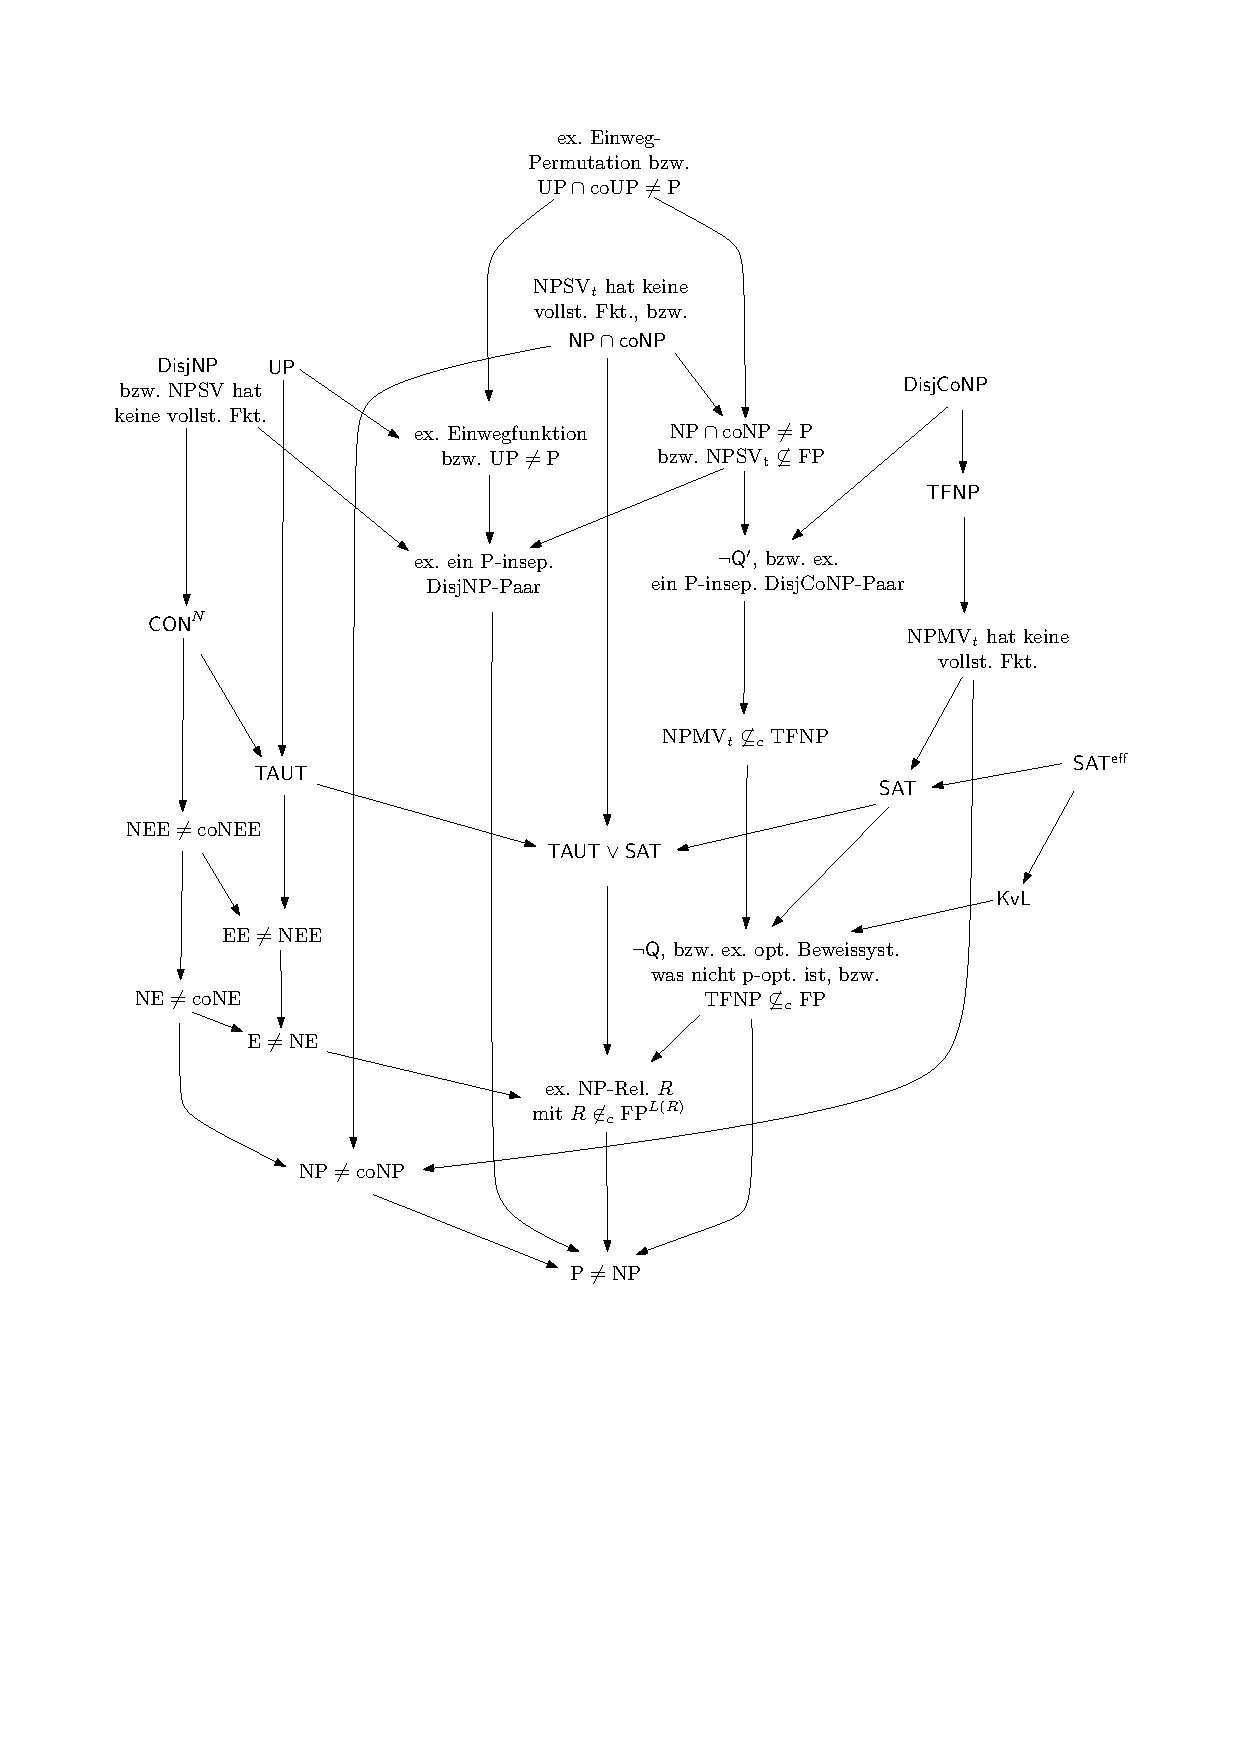
\includegraphics[page=1]{figures.pdf}
    \caption{Bekannte (relativierenden) Implikationen zwischen den betrachteten Hypothesen und weiteren Aussagen. Satz~\ref{thm:figure-implications} gibt Belegstellen für jede dieser Implikationen an.}\label{fig:figure-implications}
    \forcerectofloat
\end{figure*}

In anderen Worten sagt Satz~\ref{thm:q-fenner} aus, dass es unter Annahme von $\hQ$ modulo Umcodieren nur einen einzigen SAT-Solver gibt, und insbesondere alle SAT-Solver äquivalent zum trivialen Solver sind, welcher nur alle möglichen Belegungen ausprobiert.
Satz~\ref{thm:q-messner} macht eine analoge Aussage über Beweissysteme: egal wie komplex ein Beweissystem $h$ für $\mathtt{SAT}$ ist, wir können immer einen $h$-Beweis für $\phi$ in eine erfüllende Belegung für $\phi$ (quasi ein trivialer Beweis für $\phi\in\mathtt{SAT}$) transformieren. Damit ist auch leicht zu sehen, dass $\hQ\Rightarrow \neg\hSAT$, zumindest im unrelativierten Fall.

In Abschnitt~\ref{sec:q-vs-search} werden wir sehen, dass sich die obigen Charakterisierungen auf weitere (aber möglicherweise nicht alle) vollständigen NP-Relationen generalisiert, womit insbesondere auch die beiden Charakterisierungen von \citeauthor{fenner_inverting_2003} bzw. \citeauthor{kobler_is_2000} zu einer \emph{relativierbaren} Variante verallgemeinert werden.
Mit dieser Verallgemeinerung ist es dann auch für uns möglich, $\hQ$ formal in das Pudláksche Programm (u.a. durch $\hQ\Rightarrow \neg\hSAT$) einzuordnen. Hierfür führen wir jetzt schon den Begriff eines Standardbeweissystems bezüglich einer NP-Relation formal ein.

\begin{definition}[Standardbeweissystem einer NP-Relation]
    Sei $R$ eine NP-Relation. Wir definieren bezüglich $R$ das \emph{Standardbeweissystem} $\mathit{std}_R$ für $\Proj(R)$ wie folgt:
    \[ \mathit{std}_R(w) \defeq \begin{cases} x & \text{wenn $w=(x,y)$ und $(x,y)\in R$,}\\
    \bot & \text{sonst}.\end{cases} \qedhere \] 
\end{definition}
Damit ist, wie durch die Formulierung oben suggeriert, $\mathit{sat}=\mathit{std}_{\mathtt{rSAT}}$.
Insbesondere ist für jede NP-Relation $R$ das Standardbeweissystem $\mathit{std}_R$ für $\Proj(R)$ ehrlich, optimal, und hat kurze Beweise.
Beachte, dass sich aufgrund der speziellen Form der Beweise von Standardbeweissystemen die $\P$-Simulation knapper formulieren lässt:
\begin{observation}\label{obs:simulation-of-spps}
    Sei $R$ eine NP-Relation, und $h$ ein Beweissystem für $\Proj(R)$. Folgende Aussagen sind äquivalent:
    \begin{enumerate}
        \item $\mathit{std}_R$ $\P$-simuliert $h$.
        \item Es existiert Funktion $g\in\FP$, sodass
            \[ h(w)=x \implies \mathit{std}_R(x, g(w))=x \quad\text{(bzw. äquivalent $(x, g(w))\in R$)}. \]
    \end{enumerate}
\end{observation}
\begin{proof}
    \begin{prooflist}
    (1)$\implies$(2): Wenn $\mathit{std}_R$ das Beweissystem $h$ $\P$-simuliert, dann existiert eine Funktion $\pi\in\FP$ sodass $h(w)=x\rightarrow \mathit{std}_R(w)=x$ gilt.
    Haben wir also einen $h$-Beweis $w$ für $x$ gegeben, dann muss $\pi(w)$ von der Form $(x, z)$ mit $z\in\Sigma^*$ und $(x,z)\in R$ sein. Insbesondere können wir dann eine Funktion $g\in\FP$ angeben, sodass $g(w)$ die zweite Komponente von $\pi(w)$ ausgibt. Dann gilt $\mathit{std}_R(x, g(w))=x$.

    (2)$\implies$(1): Haben wir eine solche Funktion $g\in\FP$ gegeben, dann realisiert $\pi(w)=(h(w), g(w))$ die $\P$-Simulation bzw. Reduktion $h\leqmp \mathit{std}_R$.
    \end{prooflist}
\end{proof}

Bevor wir nun mit einer Diskussion zwischen Karp-Vollständigkeit und Levin-Vollständigkeit fortsetzen, machen wir folgende Beobachtung über $\hQ$ und der Ordnung der Simulation vs. $\P$-Simulation. Diese Beobachtung machen schon \textcite{kobler_is_2000}, aber deren Beweis (vgl. \cite[Thm.~5.2]{messner_simulation_2001}) relativiert insbesondere nicht. Wir zeigen die Aussage hier über eine nichttriviale Verallgemeinerung, welche insbesondere relativiert.
\begin{theorem}\label{thm:q-simulation}
    Folgende Aussagen sind äquivalent:
    \begin{enumerate}
        \item $\hQ$.
        \item Sei $L$ eine Menge und $h$, $g$ je Beweissysteme für $L$. Es gilt
            \[ \text{$h$ simuliert $g$} \iff \text{$h$ $\P$-simuliert $g$}. \]
        \item Für jedes Beweissystem $h$ gilt: $h$ ist optimal $\iff$ $h$ ist $\P$-optimal.
        \item Jedes ehrliche Beweissystem $h$ ist $\P$-optimal.
    \end{enumerate}
\end{theorem}
\begin{proof}
    \begin{prooflist}
    \item (1)$\implies$(2): Die Richtung von rechts nach links ist klar. Wir zeigen die andere Richtung. Nach Voraussetzung kann $h$ das Beweissystem $g$ simulieren, das heißt es existiert eine (nicht notwendigerweise effiziente) Funktion $\pi$ sodass $g(w)=h(\pi(w))$, und gleichzeitig ist $|\pi(w)|\leq q(|w|)$ für ein geeignetes Polynom $q$.

Betrachte folgende Multifunktion $f$:
\[ \fset{}f(w) \defeq  \{ y \mid \exists y\in\Sigma^{\leq q(|w|)}, g(w)=h(y) \}. \]
Es lässt sich leicht zeigen, dass $f\in\NPMV$, über einen geeigneten NPTM-Transduktor. 
Es ist sogar $f\in\NPMV_t$, denn für jedes $w\in\Sigma^*$ gilt mindestens $\pi(w)\in \fset{}f(w)$.

Mit $\hQ$ gilt nach Satz~\ref{thm:q-orig} also $f\in\NPMV_t\subseteqc \FP$, also existiert eine Funktion $f'\in\FP$ welche eine Verfeinerung von $f$ ist. Diese Funktion übersetzt $g$-Beweise $w$ für $x$ effizient in $h$-Beweise für $x$: 
Sei $g(w)=x$, dann gilt
\[ f'(w) = y \quad\text{mit } y\in\fset{}f(w), \text{ also gilt } y\in\Sigma^{\leq q(|w|)}, x=g(w)=h(y). \]
Damit ist $h(f'(w))=x$ bzw. $f'(w)$ ein $h$-Beweis für $x$, wie gewünscht.

\item (2)$\implies$(3): Klar.

\item (3)$\implies$(4): Klar, denn wenn $h$ ehrlich ist, dann hat es insbesondere auch kurze Beweise. Also ist $h$ auch optimal (Beobachtung~\ref{obs:super-ps-sind-opt}), und nach (3) dann auch $\P$-optimal.

\item (4)$\implies$(1): Wir zeigen, dass mit Voraussetzung (4) auch $\TFNP\subseteqc \FP$ gilt, was nach Satz~\ref{thm:q-orig} äquivalent zu $\hQ$ ist. Sei hierfür $R\in\TFNP$ gegeben.

    Das Standardbeweissystem $\mathit{std}_R$ für $\Sigma^*$ ist ehrlich, also nach (4) auch ein $\P$-optimales Beweissystem für $\Sigma^*$. Beachte, dass auch die Identitätsfunktion $\mathrm{id}$ ein Beweissystem für $\Sigma^*$ ist. Also kann $\mathit{std}_R$ das Beweissystem $\mathrm{id}$ $\P$-simulieren. Nach Beobachtung~\ref{obs:simulation-of-spps}(2) existiert also eine Funktion $g\in\FP$ sodass $\mathrm{id}(w)=x\rightarrow (x, g(w))\in R$. Da nun aber $\mathrm{id}(x)=x$ gilt $(x, g(x))\in R$, also ist $g$ eine Verfeinerung von $R$. Damit $R\inc\FP$, wie gewünscht.
    \end{prooflist}
\end{proof}

%Bevor wir nun mit einer Diskussion zwischen Karp-Vollständigkeit und Levin-Vollständigkeit fortsetzen, schließen wir diesen Einstieg mit folgender einfachen Beobachtung ab:
%\begin{observation}\label{obs:spps-honest}
    %Für jede NP-Relation $R$ ist das Standardbeweissystem $\mathit{std}_R$ für $\Proj(R)$ ehrlich, optimal, und hat kurze Beweise.
%\end{observation}
%\begin{proof}
    %Nachdem $R$ polynomiell längenbeschränkt ist, folgt sofort dass $\mathit{std}_R$ kurze Beweise hat. 
    %Nach Beobachtung \ref{obs:super-ps-sind-opt} damit auch optimal.
    %Insbesondere hat $\mathit{std}_R$ \emph{nur} polynomiell längere Beweise, also ist $\mathit{std}_R$ ehrlich.
%\end{proof}

\section{Karp-Vollständigkeit vs. Levin-Vollständigkeit}\label{sec:karp-vs-levin}

Wir wiederholen hier erneut die zentrale offene Frage und Vermutung aus Abschnitt~\ref{sec:levin}:

\begin{reptheorem}{Frage}{question:kvl}
    Sei $R$ eine NP-Relation.
Wenn $\Proj(R)$ eine $\leqmp$-vollständige Menge für $\NP$ ist, ist dann auch $R$ eine $\leqlp$-vollständige NP-Relation für $\FNP$?
\end{reptheorem}

\begin{reptheorem}{Vermutung}{conj:kvl}[$\mathsf{KvL}$]
    Es existiert eine NP-Relation $R$ sodass $\Proj(R)$ $\leqmp$-vollständig für $\NP$ ist, aber $R$ ist nicht $\leqlp$-vollständig für $\FNP$.
\end{reptheorem}

Zunächst sei hier noch einmal hervorgehoben, dass eine negative Beantwortung der Frage~\ref{question:kvl}, also ein Beweis von $\mathsf{KvL}$ schwer ist. Zum einen haben wir bereits gesehen, dass ein Beweis $\mathsf{KvL}$ auch sofort $\P\neq\NP$ beweisen würde. Insbesondere ist ein relativierender Beweis von $\mathsf{KvL}$ ausgeschlossen, denn existiert ein Orakel, relativ zu diesem $\neg\mathsf{KvL}$ (z.B. ein PSPACE-vollständiges Orakel, welches $\NP$ auf $\P$ kollabiert).
Auch für eine positive Beantwortung der Frage (also ein Beweis für $\neg\mathsf{KvL}$) fehlen uns konkrete Indizien.

Wir werden uns daher im Folgenden insbesondere auf Beziehungen zwischen $\mathsf{KvL}$ und gewissen anderen Hypothesen konzentrieren.
In diesem Sinne möchte ich argumentieren, dass die obige Frage bzw. Vermutung eng mit der Hypothese $\hQ$ zusammenhängt.
Im Speziellen werden wir sehen, dass die Hypothese $\hQ$ so charakterisiert werden kann, dass sie einer Verstärkung der Vermutung $\neg\mathsf{KvL}$ entspricht.\footnote{\textcite{fenner_inverting_2003} gaben hierbei eine ähnliche Aussage an (Cor.~3: „$\hQ$ holds iff every Karp reduction from $A$ to $B$ can be extended to a Levin reduction“), es ist aber hervorzuheben, dass die Autoren von einem unüblichen Begriff von Levin-Reduktionen ausgehen, der sich von dem hier verwendeten unterscheidet. Dieser umfasst nicht eine „Rückwärts-Translation“ von Zertifikaten für $B$-Instanzen zu $A$-Instanzen, sondern eine „Vorwärts-Translation“ von Zertifikaten für $A$-Instanzen zu $B$-Instanzen.}

\begin{theorem}\label{thm:q-as-levin}
    Folgende Aussagen sind äquivalent:
    \begin{enumerate}
        \item Hypothese $\hQ$.
        \item Für jedes Paar von NP-Relationen $A, B$ gilt:
            \[ \Proj(A) \leqmp \Proj(B) \iff A \leqlp B. \]
    \end{enumerate}
\end{theorem}
\begin{proof}
    \begin{prooflist}
\item (1)$\implies$(2): Die Richtung von rechts nach links ist klar. Für die andere Richtung sei $\Proj(A) \leqmp \Proj(B)$ mit $A,B$ NP-Relationen. Sei $q$ hierbei die Zertifikatsschranke von $A$.
    Wir wollen nun eine Levin-Reduktion von $A$ auf $B$ angeben. Sei $f\in \FP$ die Funktion, welche die Reduktion $\Proj(A) \leqmp \Proj(B)$ realisiert.
    Zunächst halten wir fest, dass unter (1) das Standardbeweissystem $\mathit{std}_R$ $\P$-optimal ist, denn es ist ehrlich, also nach Satz~\ref{thm:q-simulation} auch $\P$-optimal.

    Definiere folgendes Beweissystem
    \[ h(w) = \begin{cases} x & \text{falls $w=0\langle x, y\rangle$ und $(x,y)\in A$} \\ x & \text{falls $w=1\langle x, z\rangle$ und $(f(x), z)\in B$} \\ \bot & \text{sonst}. \end{cases}\]
    Es ist leicht zu sehen, dass $h$ ein Beweissystem für $\Proj(A)$ ist.
    Also kann $\mathit{std}_R$ das Beweissystem $h$ $\P$-simulieren. Mit Beobachtung~\ref{obs:simulation-of-spps} folgt, dass eine Funktion $g$ existiert mit
    \[ h(w)=x\implies (x, g(w))\in A. \]
    Wir zeigen nun, dass $A\leqlp B$. Sei hierfür $f$ von oben die entsprechende Reduktionsfunktion.
    Es gilt
    \begin{gather*}
        (f(x), z)\in B \implies h(1\langle x, z\rangle)=x \implies (x, \underbrace{g(1\langle x, z\rangle)}_{g'(x, z)})\in A,
    \end{gather*}
    heißt mit der Translationsfunktion $g'\in\FP, g'(x,z)=g(1\langle x,z\rangle)$ können wir $B$-Zertifikate für $f(x)$ in $A$-Zertifikate für $x$ umrechnen, wie gewünscht.

\item (2)$\implies$(1): Wir zeigen $\TFNP\subseteqc \FP$; das ist nach Satz~\ref{thm:q-orig} äquivalent zu (1). Sei nun $A$ eine totale NP-Relation
    Definiere nun die NP-Relation
    \[ B \defeq \{ (x, \epsilon) \mid x\in\Sigma^* \}. \]
    Es ist leicht zu sehen das $\Proj(A)=\Sigma^*=\Proj(B)$ und dass $\Proj(A)\leqmp\Proj(B)$ über die Identitätsfunktion.
    Nach Annahme (2) lässt sich nun diese Reduktion zu einer Levin-Reduktion $A\leqlp B$ verstärken, mit Reduktionsfunktion $f\in\FP$ und  Translationsfunktion $g\in\FP$.

    Sei nun ein Wort $x\in\Sigma^*$ gegeben. Hieraus können wir effizient ein $A$-Zertifikat berechnen: es gilt $(f(x),\epsilon)\in B$, also auch $(x, g(x, \epsilon))\in A$. Heißt, $g(x, \epsilon)$ ist unser gesuchtes $A$-Zertifikat, welches wir auch effizient berechnen können.
\end{prooflist}
\end{proof}

Beachte, dass in Aussage (2) die Implikation von rechts nach links ohnehin immer gilt. 
Damit lässt sich Aussage (2) auch so formulieren, dass jede Karp-Reduktion zu einer Levin-Reduktion verstärkt werden kann, indem zur Reduktionsfunktion $f$ eine geeignete Translationsfunktion $g$ hinzugefügt wird.
Mit dieser Charakterisierung folgt auch unmittelbar, dass $\hQ$ hinreichend für $\neg\mathsf{KvL}$ ist: ist $\Proj(A)$ $\leqmp$-vollständig, dann lässt sich jede Reduktion $\Proj(B)\leqmp \Proj(A)$ zu einer $\leqlp$-Reduktion $B\leqlp A$ verstärken; also ist $A$ $\leqlp$-vollständig.


\begin{corollary}\label{cor:kvl-implies-q}
    $\hQ\implies \neg\mathsf{KvL}$.
\end{corollary}
%\begin{proof}
    %Wir starten mit der Voraussetzung $\hQ$.
    %Wir wollen nun $\neg\mathsf{KvL}$ zeigen. Sei hierfür $R$ eine beliebige NP-Relation sodass $\Proj(R)$ $\leqmp$-vollständig für $\NP$ ist.
    %Damit gilt also schon für alle weiteren NP-Relationen $A$, dass $\Proj(A)\leqmp\Proj(R)$.
    %Nach Satz~\ref{thm:q-as-levin} gilt nun $A\leqlp R$. Also ist $R$ auch $\leqlp$-vollständig für $\FNP$, wie gewünscht und wir haben $\neg\mathsf{KvL}$ gezeigt.
%\end{proof}

\subsection*{P-Quasi-Simulation}

Was sind natürliche notwendige Bedingungen für die Hypothese $\mathsf{KvL}$? Diese Frage erscheint tatsächlich wesentlich schwieriger als gedacht. Insbesondere scheint es unklar, ob aus irgend einer von Pudláks Hypothesen die Aussage $\mathsf{KvL}$ folgt.

Um uns dieser Frage dennoch zu nähern, beginnen wir zunächst, die Hypothese $\mathsf{KvL}$ auf weitere Weisen zu charakterisieren. Es ist intuitiv ersichtlich, dass für eine feste Sprache $L$ die NP-Relationen für $L$, die ehrlichen Beweissysteme für $L$, und die NPTMs, welche $L$ entscheiden, alle im breitesten Sinn „Zertifikatsschemata“ sind, und alle diese Berechnungsmodelle untereinander umgeschrieben werden können: jede NP-Relation $R$ induziert ein ehrliches Beweissystem $\mathit{std}_R$, jedes ehrliche Beweissystem $h$ induziert eine NPTM $N$ mit $L(N)=L$ (rate einen $h$-Beweis polynomieller Länge), und jede NPTM $N$ mit $L(N)=L$ induziert eine NP-Relation für $L$ ($w$ ist eine Lösung für $x$ wenn $w$ ein akzeptierender Rechenweg auf $N(x)$ ist). Insbesondere ist für ein ehrliches Beweissystem $h$ die Umkehrrelation $h^{-1}=\{(x,w) \mid h(w)=x \} $ eine NP-Relation für $\img(h)$.

Wir wollen nun die existierende $\leqlp$-Ordnung auf den NP-Relationen aufgreifen, und diese auf die ehrlichen Beweissysteme übertragen. Wir definieren hierfür eine abgeschwächte Variante der $\P$-Simulation, welche der $\leqlp$-Reduktion nachempfunden ist.
\begin{definition}
    Seien $h,h'$ Beweissysteme für $L$. Das Beweissystem $h$ \emph{$\P$-quasi-simuliert} $h'$ falls Funktionen $f,g\in\FP$ existieren sodass
    \begin{enumerate}
        \item $x\in L \iff f(x)\in L$,
        \item $ h'(w)=f(x) \implies h(g(x, w)) = x. $\qedhere
    \end{enumerate}
    %Kann das Beweissystem $h$ jedes Beweissystem $h'$ für $L$ effektiv $\P$-simulieren, dann ist $h$ \emph{effektiv $\P$-optimal}.
\end{definition}
In anderen Worten, falls $h$ das Beweissystem $h'$ $\P$-quasi-simuliert, dann kann $h$ zwar nicht \emph{jeden} $h'$-Beweis $w$ für $x\in L$ in einen $h$-Beweis für (das gleiche) $x$ effizient umrechnen, es kann aber zumindest alle \emph{relevanten} $h'$-Beweise effizient umrechnen, nämlich für jedes $x\in L$ die $h'$-Beweise für $f(x)$ in $h$-Beweise für $x$.
%Anstelle „$h$ $\P$-simuliert effektiv $h'$“ ließe sich äquivalent auch $h^{-1}\leqlp h'^{-1}$ schreiben. Beachte, dass die Relation $h^{-1}$ nur Lösungen mit ihren Beweisen reliert.
Die $\P$-Quasi-Simulation ist reflexiv und transitiv, und sie 
liegt insbesondere zwischen Simulation und $\P$-Simulation: $\P$-Simulation impliziert $\P$-Quasi-Simulation impliziert Simulation.
Ferner ist diese Art von Simulation \emph{effektiv}, in dem Sinn dass die $\P$-invertierbaren Beweissysteme selbst unter $\P$-Quasi-Simulation abgeschlossen sind.

Es ist intuitiv ersichtlich, dass $\P$-quasi-Simulation auf ehrlichen Beweissystemen das Analog der $\leqlp$-Reduktion auf NP-Relationen darstellt. Wir können folgende Beobachtung festhalten:
\begin{observation}\label{obs:p-quasi-sim-vs-leqlp}
    Sei $L\in\NP$, seien $h, h'$ zwei ehrliche Beweissysteme für $L$, und seien $R, R'$ zwei NP-Relationen für $L$.
    \begin{enumerate}
        \item $h^{-1}\leqlp h'^{-1} \iff \text{$h$ kann $h'$ $\P$-quasi-simulieren.}$
        \item $R\leqlp R' \iff \text{$\mathit{std}_R$ kann $\mathit{std}_{R'}$ $\P$-quasi-simulieren.}$
    \end{enumerate}
\end{observation}
\begin{proof}
    \begin{prooflist}
    \item Zu (1): Wir haben
        \begin{gather*}
            h^{-1}\leqlp h'^{-1} \iff \exists f,g\in\FP.\, [(f(x), w)\in h'^{-1} \rightarrow (x, g(x, w))\in h^{-1}]\\
            \iff \exists f,g\in\FP.\, [h'(w)=f(x) \rightarrow h(g(x, w))=x]\\
            \iff \text{$h$ kann $h'$ $\P$-quasi-simulieren,}
        \end{gather*}
        wobei hier die existenziell quantifizierte Variable $f$ nur über Reduktionsfunktionen von $L$ auf $L$ reichen soll.
    \item Zu (2): Ähnlich wie (1), nur etwas aufwändiger. Wir haben
        \begin{gather*}
            R\leqlp R' \iff \exists f,g\in\FP.\, [(f(x), w)\in R' \rightarrow (x, g(x, w))\in R]\\
            \iff \exists f,g\in\FP.\, [\mathit{std}_{R'}(f(x), w)=f(x) \rightarrow \mathit{std}_R(x, g(x, w))=x\\
            \iff \exists f,g'\in\FP.\, [\mathit{std}_{R'}(w')=f(x) \rightarrow \mathit{std}_R(g'(x, w'))=x\\
            \iff \text{$\mathit{std}_{R}$ kann $\mathit{std}_{R'}$ $\P$-quasi-simulieren,}
        \end{gather*}
        wobei wieder die existenziell quantifizierte Variable $f$ nur über Reduktionsfunktionen von $L$ auf $L$ reichen soll.
    \end{prooflist}
\end{proof}

Die intuitive Aussage von $\neg\mathsf{KvL}$ „Alle NP-Relationen für NP-vollständige Sprache $L$ sind im Wesentlichen gleich“ überträgt sich nun auch auf ehrliche Beweissysteme:
\begin{theorem}\label{thm:kvl-ps}
    Folgende Aussagen sind äquivalent:
    \begin{enumerate}
        \item Aussage $\neg\mathsf{KvL}$.
        \item Für jede $\leqmp$-vollständige Menge $L\in\NP$ gilt: Wenn $R, R'$ zwei NP-Relationen für $L$ sind, dann
            \[ R \leqlp R'. \]
        \item Für jede $\leqmp$-vollständige Menge $L\in\NP$ gilt: Wenn $h, h'$ zwei ehrliche Beweissysteme für $L$ sind, dann
            \[  \text{$h$ $\P$-quasi-simuliert $h'$}. \]
        \item Für eine $\leqlp$-vollständige NP-Relation $R$ gilt: Wenn $R'$ eine NP-Relation für $\Proj(R)$ ist, dann
            \[ R \leqlp R'. \]
    \end{enumerate}
\end{theorem}
\begin{proof}
    \begin{prooflist}
        \item (1)$\implies$(2): Klar, denn mit (1) ist $R'$ $\leqlp$-vollständig.
        \item (2)$\implies$(4): Klar, ist ja $\mathtt{rSAT}$ $\leqlp$-vollständig.
        \item (4)$\implies$(1): Sei $Q$ eine NP-Relation, wobei $\Proj(Q)$ $\leqmp$-vollständig für $\NP$ ist. Wir werden zeigen, dass $R\leqlp Q$, wobei dann auch $Q$ $\leqlp$-vollständig ist (Beob.~\ref{lemma:fnp-completeness}), wie gewünscht.
        Die Argumentation verläuft hierbei ähnlich wie bei Satz~\ref{thm:q-as-levin}. Sei $f\in\FP$ die Funktion, welche $\Proj(R)\leqmp \Proj(Q)$ realisiert.
        Sei nun
        \[ R' = \{ (x, 0y) \mid (x,y)\in R \} \cup \{ (x, 1z) \mid (f(x), z)\in Q \}. \]
        Es lässt sich leicht zeigen, dass $R'$ eine NP-Relation für $\Proj(R)$ ist.
        Nach (4) gilt nun $R \leqlp R'$. Ebenso gilt $R'\leqlp Q$, denn wir haben
\[ (f(x), z)\in Q \implies (x, \underbrace{1z}_{\mathclap{g(x,z)}})\in R', \]
        also realisiert $f$ als Reduktionsfunktion und $g(x,z)\defeq 1z$ als Translationsfunktion die Levin-Reduktion $R'\leqlp Q$. Damit gilt $R\leqlp R'\leqlp Q$ wie gewünscht.
        \item (2)$\iff$(3): Einfach mit Beobachtung~\ref{obs:p-quasi-sim-vs-leqlp} nachweisbar.
    \end{prooflist}
\end{proof}

Als Korollar erhalten wir dabei insbesondere folgende Aussage, welche $\mathsf{KvL}$ mit Standardbeweissystemen von $\leqlp$-vollständigen NP-Relationen in Beziehung setzt:
\begin{corollary}\label{cor:kvl-spps}
    Sei $R$ eine NP-Relation, sodass $R$ $\leqlp$-vollständig ist.
    Folgende Aussagen sind äquivalent:
    \begin{enumerate}
        \item Aussage $\neg\mathsf{KvL}$.
        \item Für alle ehrlichen Beweissysteme $h$ mit $\img(h)=\Proj(R)$ gilt
        \[  \text{$\mathit{std}_R$ $\P$-quasi-simuliert $h$}. \]
    \end{enumerate}
\end{corollary}
\begin{proof}
    \begin{prooflist}
    \item (1)$\implies$(2): Klar, denn $\mathit{std}_R$ ist ehrlich, und mit Satz~\ref{thm:kvl-ps}(3) kann $\mathit{std}_R$ damit $h$ auch $\P$-quasi-simulieren.

    \item (2)$\implies$(1): Wir zeigen die Aussage von Satz~\ref{thm:kvl-ps}(4), womit auch $\neg\mathsf{KvL}$ bzw (1) gilt. Sei hierfür $R'$ eine NP-Relation für $\Proj(R)$. Mit (2) wissen wir dass $\mathit{std}_R$ das Beweissystem $\mathit{std}_{R'}$ $\P$-quasi-simulieren kann. Mit Beobachtung~\ref{obs:p-quasi-sim-vs-leqlp}(2) folgt $R\leqlp R'$.
    \end{prooflist}
\end{proof}

Unter dieser Charakterisierung erhalten wir einen zweiten trivialen Beweis von Korollar~\ref{cor:kvl-implies-q}: $\hQ$ ist hinreichend für $\neg\mathsf{KvL}$, denn unter Annahme von $\hQ$ ist jedes ehrliche Beweissystem $\P$-optimal, heißt auch das Standardbeweissystem $\mathit{std}_{\mathtt{rKAN}}$ für $\mathtt{KAN}$ ist $\P$-optimal (Satz~\ref{thm:q-simulation}), kann also insbesondere auch alle ehrlichen Beweissysteme $h$ $\P$-quasi-simulieren. Damit auch $\neg\mathsf{KvL}$ (Korollar~\ref{cor:kvl-spps}).

Mittels unserem Begriff der $\P$-Quasi-Simulation können wir nun auch die Hypothese $\hSAT$ auf natürliche Weise verstärken:
\begin{conjecture}[$\mathsf{SAT^{q}}$]
    Es existiert keine $\leqmp$-vollständige Menge $L$ für $\NP$ mit einem Beweissystem $h$, welches alle anderen ehrlichen Beweissysteme für $L$ $\P$-quasi-simulieren kann. 
\end{conjecture}
Diese Verstärkung ist am sichtbarsten, wenn wir uns überlegen, wie die Negation $\neg\hSAT$ zu $\neg\mathsf{SAT^{q}}$ in zwei Aspekten abgeschwächt wird.
Erstens der Umfang: es wird nicht mehr verlangt, dass ein Beweissystem $h$ existiert, welche \emph{alle} Beweissysteme $\P$-simulieren kann, sondern nur noch alle \emph{ehrlichen} Beweissysteme.
Zweitens die Beziehung: es wird nicht mehr $\P$-Simulation, sondern nur noch $\P$-\emph{Quasi}-Simulation vorausgesetzt.

Wir sehen nun, dass $\mathsf{SAT^{q}}$ eine Verstärkung von sowohl $\hSAT$ als auch $\mathsf{KvL}$ ist:
\begin{corollary}\label{cor:sateff-generalizes-sat}
    \begin{enumerate}
        \item $\mathsf{SAT^{q}}\implies \hSAT$
        \item $\mathsf{SAT^{q}}\implies \mathsf{KvL}$
    \end{enumerate}
\end{corollary}
\begin{proof}
    Für (1) haben wir bereits argumentiert. Wir zeigen nur noch (2) mittels Kontraposition. Unter $\neg\mathsf{KvL}$ folgt mit der Formulierung aus Korollar~\ref{cor:kvl-spps}(2), dass das Standardbeweissystem der $\leqlp$-vollständigen NP-Relation $\mathtt{rSAT}$ alle ehrlichen Beweissysteme $\P$-quasi-simulieren kann. Also hat die Menge $\mathtt{KAN}$ \emph{ein} Beweissystem, welches alle ehrlichen Beweissysteme $\P$-quasi-simulieren kann.
\end{proof}

Wir haben damit also je eine notwendige ($\neg\hQ$) und eine hinreichende Hypothese ($\mathsf{SAT^{q}}$) für $\mathsf{KvL}$. Durch die Charakterisierung von $\neg\mathsf{KvL}$ über Beweissysteme ergibt sich durch Korollar~\ref{cor:kvl-spps} eine interessante Ähnlichkeit zur Hypothese $\hQ$. Wir wollen diese beiden Hypothesen im Folgenden kurz gegenüberstellen.
Zur Anschaulichkeit beziehe ich mich hierbei auf die NP-Relation $\mathtt{rSAT}$. (Durch Ergebnisse im nächsten Abschnitt wird klar, dass sich dieses Argument auch auf $\mathtt{rKAN}$ relativierend überträgt.)
Wir haben
\begin{itemize}[midpenalty=10000]
    \item $\hQ$ genau dann wenn $\mathit{sat}$ jedes ehrliche Beweissystem $\P$-simulieren kann (Satz~\ref{thm:q-fenner}),\sidenote{Satz~\ref{thm:q-fenner} macht zwar nur Aussagen über NPTMs, aber es ist leicht zu sehen, dass diese mit den ehrlichen Beweissystemen identifiziert werden können. Vgl. auch Satz~\ref{thm:q-fenner-generalized}.}
    \item $\neg\mathsf{KvL}$ genau dann wenn $\mathit{sat}$ jedes ehrliche Beweissystem $\P$-quasi-simulieren kann (Korollar~\ref{cor:kvl-spps}).
\end{itemize}
Damit wird deutlich, dass die die Hypothesen $\hQ$ und $\neg\mathsf{KvL}$ äquivalent sind, falls die $\P$-Quasi-Simulation genauso stark ist wie die $\P$-Simulation.

%Insbesondere vermute ich, dass möglicherweise sogar $\hQ\Leftrightarrow\neg\mathsf{KvL}$ gelten könnte. Die Richtung von links nach rechts haben wir bereits in Korollar~\ref{cor:kvl-implies-q} gesehen, und ist ferner in der hier genannten Charakterisierung trivial. Für die Richtung von rechts nach links möchte ich nun plausibilisieren, dass $\neg\mathsf{KvL}\land\neg\hQ$ zu einem Widerspruch führt.

%Unter Annahme von $\neg\hQ$ folgt nach Satz~\ref{thm:q-fenner}, dass das Standardbeweissystem $\mathit{sat}$ von $\mathtt{rSAT}$ ein bestimmtes ehrliches Beweissystem $h$ nicht $\P$-simulieren kann.
%Wir haben also für alle Funktionen $f\in\FP$ 
%\begin{equation} h(w)=\psi \rlap{\hspace*{2pt}\raisebox{2.3pt}{$\quad\not$}}\implies  \text{$f(w)$ erfüllt $\psi$}.\label{eq:weak-irreducibility} \end{equation}
%In anderen Worten: obwohl wir einen $h$-Beweis $w$ für die Erfüllbarkeit der Formel $\phi$ haben, können wir nicht effizient eine erfüllende Belegung aus $w$ berechnen.

%Nun gilt aber nach Annahme auch $\neg\mathsf{KvL}$. Über Satz~\ref{thm:kvl-ps}(4) gilt, dass $\mathit{sat}$ das ehrliche Beweissystem $h$ $\P$-quasi-simulieren kann. Wir haben also zwei Funktionen $f', g'\in\FP$ sodass
%\begin{equation}\label{eq:effective-simulation} h(w)=f'(\phi) \implies \text{$g'(\phi, w)$ erfüllt $\phi$}. \end{equation}
%Beachte, dass die Funktion $f'$ notwendigerweise ungleich $\mathrm{id}$ ist. Wir können $f'$ so verstehen, dass diese $\phi$ gewissermaßen in eine einfachere Form bringt, für welche $h$-Beweise effizient verarbeitet werden können.

%Es ist also einerseits nicht möglich, aus dem $h$-Beweis $w$ effizient eine akzeptierende Belegung für $f(\phi)$ zu bestimmen, obwohl $w$ bezeugt dass $f(\phi)$ erfüllbar ist. (Ersetze in \eqref{eq:weak-irreducibility} $\psi$ mit $f(\phi)$.)
%Andererseits reicht der $h$-Beweis $w$ für $f(\phi)$ aber aus, um (zusammen mit der Information $\phi$) effizient wieder eine erfüllende Belegung für $\phi$ zu berechnen. 
%Diese Argumentation \emph{plausibilisiert} zwar einen Widerspruch, bzw. dass $\neg\hQ\land\neg\mathsf{KvL}$ wahrscheinlich falsch ist, ist aber natürlich kein solcher. Die Umkehrung von Korollar~\ref{cor:kvl-implies-q} bleibt offen.

Dennoch bleiben weitere Fragen offen, die wir hier aus Platzgründen nicht weiter verfolgen werden. 
Zum einen zur Charakterisierung von $\mathsf{KvL}$:
Wir konnten zwar $\mathsf{KvL}$ unter anderem als Aussage über Beweissysteme formulieren, aber sind auch noch weitere äquivalente Charakterisierungen möglich, z.B. ähnlich wie bei $\hQ$?

Zum anderen die Beziehungen zwischen $\mathsf{KvL}$ und anderen Hypothesen bzw. Annahmen.
Gibt es natürliche (z.B. kryptographische) Annahmen, welche hinreichend für $\mathsf{KvL}$ sind? Wie ist die Beziehung zu den anderen Pudlákschen Hypothesen? Wie verhält sich insbesondere $\hSAT$ zu $\mathsf{SAT^{q}}$? 
Diese Fragen werden wir zum Teil in Kapitel~\ref{chap:orakel} klären; dort wird ein Orakel konstruiert, welches zeigt, dass selbst unter der Annahme von $\hDisjNP\land\hUP$ es nicht möglich ist, mit relativierenden Beweismethoden auf $\mathsf{KvL}$ zu schließen.
Wir kommen hierauf am Ende dieses Kapitels noch einmal zurück.

Insgesamt ist durch die vorherigen Überlegungen aber ein erster Schritt getan, die Beziehung zwischen Levin- und Many-one-Vollständigkeit über die Vermutung $\mathsf{KvL}$ im Kontext des Pudlákschen Programms einzuordnen.
Weitere Forschung in diese Richtung erscheint vielversprechend.

\section{Hypothese $\hQ$ und Suchprobleme}\label{sec:q-vs-search}

Wie im Einstieg des Kapitels angesprochen, geben \textcite{fenner_inverting_2003} bzw. \textcite{kobler_is_2000} äquivalente Charakterisierungen der Hypothese $\hQ$ an, welche sich im Wesentlichen auf auf der $\leqlp$-Vollständigkeit von $\mathtt{rSAT}$ aufbauen (Satz~\ref{thm:q-fenner} und \ref{thm:q-messner}).
Wir wiederholen hier noch einmal die Aussagen, aber mit einer etwas abstrakteren Notation.
Wie schon angesprochen, können für eine feste Menge $L$ die ehrlichen Beweissysteme für $L$ mit den NPTMs identifiziert werden, welche $L$ entscheiden.
So können wir die anfangs genannten Charakterisierung von \citeauthor{fenner_inverting_2003} stattdessen folgendermaßen notieren:
\begin{reptheorem}{Satz}{thm:q-fenner}[\cite{fenner_inverting_2003}]
    Es gilt $\hQ$ genau dann wenn $h\leqmp\mathit{sat}$ für jedes ehrliche Beweissystem $h$ für $\mathtt{SAT}$. 
\end{reptheorem}
Die Charakterisierung von \citeauthor{kobler_is_2000} können wir auf ähnliche Weise über Standardbeweissysteme von NP-Relationen schreiben.
\begin{reptheorem}{Satz}{thm:q-messner}[\cite{kobler_is_2000}]
    Es gilt $\hQ$ genau dann wenn das Standardbeweissystem $\mathit{std}_\mathtt{rSAT}$ $\P$-optimal ist.
\end{reptheorem}

Diese beiden Charakterisierungen wollen wir im Folgenden verallgemeinern und von $\mathtt{rSAT}$ auf beliebige $\leqlp$-vollständige NP-Relationen $R$ übertragen. 
Hieraus ergibt sich schon unmittelbar der technische Beitrag, dass dann diese Charakterisierungen auch in einer relativierten Umgebung angewendet werden können, um z.B. ein geeignetes Orakel zu konstruieren, was $\hQ$ von anderen Hypothesen trennt.

Das ist für den zweiten Satz~\ref{thm:q-messner} ohne weitere zusätzliche Bedingungen möglich. Beachte, dass sich der hier präsentierte Beweis maßgeblich von dem ursprünglichen Beweis von \textcite[vgl.][Thm.~5.2]{messner_simulation_2001} unterscheidet, und insbesondere ohne sein (nichtrelativierendes) Padding-Argument auskommt.
\begin{theorem}\label{thm:q-messner-generalized}
    Sei $R$ eine beliebige $\leqlp$-vollständige NP-Relation.
    Folgende Aussagen sind äquivalent:
    \begin{enumerate}
        \item Aussage $\hQ$.
        \item Das Standardbeweissystem $\mathit{std}_R$ ist $\P$-optimal.
    \end{enumerate}
\end{theorem}
\begin{proof}
    \begin{prooflist}
    \item (1)$\implies$(2): 
        Das Standardbeweissystem $\mathit{std}_R$ ist ehrlich. Nach Satz~\ref{thm:q-simulation} ist $\mathit{std}_R$ damit $\P$-optimal.

    \item (2)$\implies$(1): Wir zeigen die Aussage, dass $\TFNP\subseteqc\FP$.  Nach Satz~\ref{thm:q-orig} ist das äquivalent zu $\hQ$. Sei hierfür ein solches $Q\in\TFNP$ gegeben

    Nachdem $R$ $\leqlp$-vollständig ist, haben wir Funktionen $f,g\in\FP$ mit
    \[ x\in \Proj(Q)\iff  f(x)\in\Proj(R), \quad (f(x), z)\in R\implies (x,g(x,z))\in Q. \]
    Definiere nun
    \[ h(w) = \begin{cases} f(x) & \text{wenn $w=0x$}\\ x & \text{wenn $w=1\langle x, y\rangle$ und $(x,y)\in R$} \\  \bot & \text{sonst} \end{cases}.\]
    Es ist leicht zu sehen, dass $h$ ein Beweissystem für $\Proj(R)$ ist, denn insbesondere gilt $f(x)\in\Proj(R)$ für jedes $x\in\Sigma^*$.
    Nach (2) gilt also $h\leqmp \mathit{std}_R$. Mit Beobachtung~\ref{obs:simulation-of-spps} haben wir eine Funktion $r\in\FP$, sodass
    \[ h(w)=x \implies (x, r(w))\in R. \]
    Damit gilt insbesondere
    \[ h(0x)=f(x)\implies (f(x), r(0x))\in R \implies (x, \underbrace{g(r(0x))}_{q(x)})\in Q. \]
    Damit ist $q(x) = g(r(0x))$, $q\in\FP$ eine Verfeinerung von $Q$, wie gewünscht.
\end{prooflist}
\end{proof}


Die andere Charakterisierung von \citeauthor{fenner_inverting_2003} ist umfangreicher.
Zunächst ist klar, dass „$h\leqmp\mathit{std}_R$ für alle ehrlichen Beweissysteme“ schwächer ist als „$h\leqmp\mathit{std}_R$ für alle Beweissysteme“, was ja nach vorigem Satz äquivalent zu $\hQ$ ist.
Tatsächlich gilt die Umkehrung scheinbar nicht für alle $\leqlp$-vollständigen NP-Relationen $R$. 
Die Autoren zeigen diese Umkehrung für die NP-Relation $\mathtt{rSAT}$, und nutzen hierbei die Eigenschaft aus, dass die entsprechenden Reduktionsfunktionen alle $\P$-invertierbar sind, bzw. in anderen Worten, die $\leq_\mathrm{L,1,i}^\mathrm p$-Vollständigkeit von $\mathtt{rSAT}$.

Wir werden im Folgenden diese Voraussetzung abschwächen, und betrachten dabei folgende Verstärkung der $\leqmp$-Reduktion.
\begin{definition}[Ehrliche Levin-Reduzierbarkeit]
    Seien $Q, R$ zwei NP-Relationen. Wir sagen dass \emph{$Q$ sich auf $R$ ehrlich Levin-reduzieren lässt}, bzw. $Q\leq_\mathrm{L,h}^\mathrm p R$ wenn $Q\leqlp R$, und die zugehörige Reduktionsfunktion $f$ ehrlich ist.

    Definiere $\leq_\mathrm{L,h}^\mathrm p$-Vollständigkeit entsprechend.
\end{definition}
Beachte, dass $\leq_\mathrm{L,h}^\mathrm p$ zwischen $\leqlp$ und $\leq_\mathrm{L,1,i}^\mathrm{p}$ liegt:
\[ Q\leq_\mathrm{L,1,i}^\mathrm{p} R \implies Q\leq_\mathrm{L,h}^\mathrm p R \implies Q\leqlp R. \]
Damit impliziert $\leq_\mathrm{L,1,i}^\mathrm{p}$-Vollständigkeit eine  $\leq_\mathrm{L,h}^\mathrm p$-Vollständigkeit, und diese eine $\leqlp$-Vollständigkeit.

Mit dem Begriff der ehrlichen Reduzierarkeit können wir den vorigen Beweis von Satz~\ref{thm:q-messner-generalized} erweitern, womit wir Satz~\ref{thm:q-fenner} generalisieren und relativieren. 
\begin{theorem}\label{thm:q-fenner-generalized}
    Sei $R$ eine beliebige $\leq_\mathrm{L,h}^\mathrm p$-vollständige NP-Relation.
    Folgende Aussagen sind äquivalent:
    \begin{enumerate}
        \item Aussage $\hQ$.
        \item Das Standardbeweissystem $\mathit{std}_R$ ist $\P$-optimal.
        \item Für jedes ehrliche Beweissystem $h$ für $\Proj(R)$ gilt $h\leqmp \mathit{std}_R$.
    \end{enumerate}
\end{theorem}
\begin{proof}
    \begin{prooflist}
    \item (1)$\implies$(2): Klar, nach Satz~\ref{thm:q-simulation} ist mit (1) das Beweissystem $\mathit{std}_R$ $\P$-optimal.

        \item (2)$\implies$(3): Klar.

        \item (3)$\implies$(1): Analog wie bei Satz~\ref{thm:q-messner-generalized}.
            Wir zeigen wieder die Aussage, dass $\TFNP\subseteqc\FP$. Sei hierfür ein solches $Q\in\TFNP$ gegeben.
    Nachdem $R$ $\leqlp$-vollständig ist, haben wir Funktionen $f,g\in\FP$, welche $Q\leqlp R$ realisieren.
    %\[ x\in \Proj(Q)=\Sigma^*\implies  f(x)\in\Proj(R), \quad (f(x), z)\in R\implies (x,g(x,z))\in Q. \]
    Definiere nun
    \[ h(w) = \begin{cases} f(x) & \text{wenn $w=0x$}\\ x & \text{wenn $w=1\langle x, y\rangle$ und $(x,y)\in R$} \\  \bot & \text{sonst} \end{cases}.\]
    Es ist leicht zu sehen, dass $h$ ein Beweissystem für $\Proj(R)$ ist.
    Insbesondere ist $h$ ehrlich, denn $f$ ist ehrlich.
    Damit gilt mit (3), dass $h\leqmp \mathit{std}_R$; mit Beobachtung~\ref{obs:simulation-of-spps} existiert dann eine Funktion $r\in\FP$, sodass
    $h(w)=x \rightarrow (x, r(w))\in R$.
    Damit ist $q(x) = g(r(0x))$, $q\in\FP$ eine Verfeinerung von $Q$, wie gewünscht.
    \end{prooflist}
\end{proof}

Wir fassen kurz den aktuellen Stand zusammen. Sei $R$ eine NP-Relation. 
Wir haben nun folgendes Bild:

\begin{center}
\begin{tikzpicture}[node distance=2cm, every node/.style={inner xsep=10pt}]
    \node (A) {$\hQ$};
    \node (B) [right=of A] {$\mathit{std}_R$ ist $\P$-opt.};
    \node (C) [right=of B, align=center] {$h \leqlp\mathit{std}_R$ für alle\\ ehrl. Beweissyst. $h$ für $\Proj(R)$};

    \draw[implies-,double equal sign distance,bend left=30] ([yshift=5pt]A.east)  to node[above] {\it\small falls $R$ Levin-vollst.} ([yshift=5pt]B.west);
    \draw[implies-,double equal sign distance,bend left=30] ([yshift=5pt]B.east)  to node[above] {\it\small falls $R$ ehrlich Levin-vollst.} ([yshift=5pt]C.west);

    \draw[-implies,double equal sign distance,bend right=30] ([yshift=-5pt]A.east)  to node[above] {} ([yshift=-5pt]B.west);
    \draw[-implies,double equal sign distance,bend right=30] ([yshift=-5pt]B.east)  to node[below] {} ([yshift=-5pt]C.west);

    \draw[draw=none] (A.east)  -- (B.west) node[midway] {(\ref{thm:q-messner-generalized}) };
    \draw[draw=none] (B.east)  -- (C.west) node[midway] {(\ref{thm:q-fenner-generalized}) };
\end{tikzpicture}
\end{center}

\subsection*{Levin-Paddability}

Die stärkere Voraussetzung an die NP-Relation $R$, dass diese \emph{ehrlich} Levin-vollständig sein muss, wollen wir hier noch einmal kurz beleuchten. Ganz ähnlich zur Berman–Hartmanis-Paddability lässt sich auch die ehrliche Levin-Vollständigkeit von $R$ äquivalent als strukturelle Eigenschaft von $R$ formulieren. Hierbei machen wir einen sehr schwachen Begriff von Paddabilty auf Suchproblemen produktiv, welcher von \textcite{messner_simulation_2001} konkret auf $\mathtt{rSAT}$ eingesetzt wurde.

Ähnlich wie bei der Berman–Hartmanis-Paddability wollen wir beliebige Instanzen $x$ zu längeren Instanzen $x'$ vergrößern. Zusätzlich verlangen wir, dass wir auch Zertifikate $y$ für $x'$ wieder zu Zertifikaten $y$ für $x$ zurückrechnen können. In anderen Worten: wir codieren „redundante Teile“ in $x$ hinein, um $x'$ zu erhalten. Für Zertifikate $y'$ für $x'$ können wir dann den Teil des Zertifikats wegwerfen, welcher sich ohnehin nur auf das redundanten Padding bezieht, und erhalten wieder ein Zertifikat $y$ für $x$. 

\begin{definition}[Levin-Paddability]\label{def:levin-paddable}
    Eine NP-Relation $R$ ist \emph{Levin-paddable} wenn 
    Funktionen $\mathit{pad}\in\FP$ und $\mathit{padsol}\in\FP$ existieren, sowie ein Polynom $r$ sodass
    \begin{enumerate}
        \item $x\in \Proj(R) \iff \mathit{pad}(x, 1^n) \in \Proj(R)$,
        \item $(\mathit{pad}(x, 1^n), y)\in R \implies (x, \mathit{padsol}(x, 1^n, y)) \in R$,
        \item $r(|\mathit{pad}(x, 1^n)|)\geq n$. (Funktion $\mathit{pad}$ ist ehrlich bzgl. der zweiten Komponente.)\qedhere
    \end{enumerate}
\end{definition}
Beachte dass wir im Gegensatz zur Berman–Hartmanis-Paddability keine Invertierbarkeit der Padding-Funktion verlangen. Wieder im Gegensatz zur Berman–Hartmanis-Paddability verlangen wir aber ein effizientes Rückrechnen der Zertifikate von gepaddeten Instanzen.

Wir sehen einfach, dass $\mathtt{rSAT}$ Levin-paddable ist: padde Formeln $\phi$ auf, indem z.B. Disjunktionen neuer Variablen hinzugefügt werden, also z.B. 
\[ \phi' = \mathit{pad}(\phi, 1^n) = \phi \lor x_k \lor x_{k+1} \lor \cdots \lor x_{k+n}, \]
wobei $k$ hinreichend groß sein soll, dass $x_k, x_{k+1}, \dots$ nicht als Variable in $\phi$ vorkommt.
%Unter jeder vernünftigen Codierung gilt $|\mathit{pad}(x, 1^n)|\geq n$.
Ist nun $w'$ eine erfüllende Belegung für $\phi'$, dann entferne alle Variablenbelegungen $x_{k}, x_{k+1}, \dots$ aus $w'$ und es ergibt sich hieraus eine erfüllende Belegung $w$ für $\phi$.

Diese Eigenschaft lässt sich auch leicht für die kanonische NP-Relation $\mathtt{rKAN}$ überprüfen, 
indem z.B. für Eingabeinstanz $x=(N, x, 1^n)$ der NPTM $N$ weitere Zustände hinzugefügt werden, welche über die Transitionsrelation von $N$ nicht erreichbar sind.
Diese Beobachtung gilt insbesondere auch im relativierten Fall.
\begin{observation}\label{obs:rkan-paddable}
    Die kanonische $\leq_\mathrm{L,1,i}^\mathrm{p}$-vollständige NP-Relation $\mathtt{rKAN}$ ist Levin-paddable.
\end{observation}

Folgendes Lemma zeigt nun, dass Levin-Paddability unter den vollständigen Relationen hinreichend für \emph{ehrliche} Vollständigkeit ist.

\begin{lemma}
    Sei $R$ eine $\leqlp$-vollständige NP-Relation. Wenn $R$ Levin-paddable ist, dann ist 
    $R$ auch $\leq_\mathrm{L,h}^\mathrm p$-vollständig.
\end{lemma}
\begin{proof}
    Sei $Q$ eine beliebige NP-Relation. Wir wollen zeigen, dass $Q\leq_\mathrm{L,h}^\mathrm p R$.
    Nachdem $R$ vollständig ist, gilt $Q\leqlp R$; sei $f,g\in\FP$ die Reduktions- bzw. Translationsfunktion welche diese Reduktion realisieren. Wir werden nun Funktionen $f', g'\in\FP$ angeben, welche die gleiche Reduktion realisieren, aber $f'$ ehrlich ist, wie gewünscht.

    Sei $\mathit{pad}, \mathit{padsol}$ die zu $R$ zugehörigen Padding-Funktionen. Definiere
    \[ f'(x) \defeq  \mathit{pad}(f(x), 1^{|x|}). \]
    Es gilt
    \[ x\in\Proj(Q) \iff f(x)\in \Proj(R) \iff \mathit{pad}(f(x), 1^{|x|})=f'(x)\in\Proj(R), \]
    wobei erste Implikation die Eigenschaft der Reduktionsfunktion $f$ ist, und die zweite aus der Definition von Levin-Paddability folgt.
    Aus der Definition von  Levin-Paddability folgt auch $r(|f'(x)|)\geq |x|$ für ein geeignetes Polynom $r$, und damit ist auch $f'$ ehrlich.

    %Definiere
    %\[ g'(x, z) \defeq  g(x, \mathit{padsol}(f(x), 1^{|x|}, z)). \]
    %Sei nun $(f'(x), z)\in R$. Die Funktion $g'$ berechnet nun ein Zertifikat $y$ für $x$: Wir haben $(\mathit{pad}(f(x), 1^{|x|}), z)\in R$, also gilt nach Levin-Paddability dass \[(f(x), \mathit{padsol}(f(x), 1^{|x|}, z))\in R,\] 
    %und nach Definition der Translationsfunktion $g$ gilt dann
    %\[(x, g(x, \mathit{padsol}(f(x), 1^{|x|}, z)))\in Q,\]
    %und das ist genau $(x, g'(x, z))\in Q$, wie gewünscht.
    Wir zeigen nun, wie sich aus $R$-Zertifikaten für $f'(x)$ wieder $Q$-Zertifikate für $x$ ausrechnen lassen können.
    Sei hierfür ein $z\in\Sigma^*$ gegeben mit $(f'(x), z)\in R$.
    Nach Definition gilt also $(\mathit{pad}(f(x), 1^{|x|}), z)\in R$, also gilt nach Levin-Paddability dass \[(f(x), \underbrace{\mathit{padsol}(f(x), 1^{|x|}, z)}_w)\in R,\] 
    und nach Definition der Translationsfunktion $g$ gilt dann
    \[(x, \underbrace{g(x, w)}_{g(x,z)})\in Q,\]
    und wir haben unser $Q$-Zertifikat für $x$. Dieses können wir effizient mittels geeignetem $g'\in\FP$ berechnen.
\end{proof}

Für die andere Richtung sehen wir, dass sich Levin-Paddability auf $\leq_\mathrm{L,h}^\mathrm p$ nach oben überträgt. 

\begin{lemma}\label{obs:invcomplete-sind-levinpaddable}
    \begin{enumerate}
        \item Gilt $\mathtt{rKAN}\leq_\mathrm{L,h}^\mathrm{p} R$, dann ist $R$ Levin-paddable (und $\leqlp$-vollständig für $\FNP$).
        \item Jede $\leq_\mathrm{L,h}^\mathrm{p}$-vollständige NP-Relation $R$ ist Levin-paddable.
    \end{enumerate}
\end{lemma}
\begin{proof}
    Aussage (2) folgt unmittelbar aus (1).

    Für (1) nutzen wir die Levin-Paddability von $\mathtt{rKAN}$ aus: übersetze Instanz $x$ von $R$ nach $\mathtt{rKAN}$, padde dort hoch, und übersetze zu $R$-Instanz $x'$ zurück. Ist dann $y'$ ein Zertifikat für $x'$, dann lässt sich dies auf ähnlichem Weg wieder zu einem Zertifikat für $x$ zurückrechnen.

    Seien $f, g$ die Reduktions- bzw. Translationsfunktion, welche $\mathtt{rKAN}\leq_\mathrm{L,h}^\mathrm p R$ bezeugen, und seinen analog $f', g'$ jene Funktionen, welche $R\leq_\mathrm{L}^\mathrm p \mathtt{rKAN}$ bezeugen. Erstere existieren nach Voraussetzung, zweitere existieren weil $\mathtt{rKAN}$ $\leq_\mathrm{L}^\mathrm p$-vollständig ist.
    Nach Voraussetzung ist $f$ ehrlich. %, und da $f'$ $\P$-invertierbar ist, ist auch $f'$ ehrlich. 
    Und nach Beobachtung~\ref{obs:rkan-paddable} existieren für $\mathtt{rKAN}$ Padding-Funktionen $\mathit{pad}_\mathtt{rKAN}$, $\mathit{padsol}_\mathtt{rKAN}$.
    Sei $q$ ein entsprechendes Polynom mit $q(|\mathit{pad}_\mathtt{rKAN}(x, 1^n)|)\geq n$, $q(|f(x)|) \geq |x|$.

    Definiere nun
    \[ \mathit{pad}_R(x, 1^n) \defeq  f(\mathit{pad}_\mathtt{rKAN}(f'(x), 1^n)). \]
    Die Zugehörigkeit zu $\Proj(R)$ bleibt erhalten:
    \begin{gather*}
        x\in \Proj(R) \iff f'(x) \in \mathtt{KAN} \iff \mathit{pad}_\mathtt{rKAN}(f'(x), 1^n) \in \mathtt{KAN}\\ \iff f(\mathit{pad}_\mathtt{rKAN}(f'(x), 1^n)) \in \Proj(R) \iff \mathit{pad}_R(x, 1^n) \in\Proj(R).
    \end{gather*}
    Ferner gilt
    \begin{align*} 
        n &\leq q(|\mathit{pad}_\mathtt{rKAN}(f'(x), 1^n)|)\\
    &\leq q(q(|f(\mathit{pad}_\mathtt{rKAN}(f'(x), 1^n)|))\\
    &=q(q(|\mathit{pad}_R(x, 1^n)|)),
    \end{align*}
    und damit ist $\mathit{pad}_R$ wie gewünscht ehrlich bzgl. $n$ (mit Polynom $q\circ q$).

    Es verbleibt noch die Funktion $\mathit{padsol}_R$ anzugeben. Nehme hierfür an, dass wir ein $y'$ gegeben haben mit $(\mathit{pad}_R(x, 1^n), y')\in R$.
    Wir können über $g, g'$ das $R$-Zertifikat $y'$ zu $R$-Zertifikat $y$ für $x$ zurück übersetzen:
    Sei $p\defeq \mathit{pad}_\mathtt{rKAN}(f'(x), 1^n)$, dann können wir $\mathit{pad}_R(x, 1^n)$ als $f(p)$ schreiben, und es gilt
    \[ (f(p), y')\in R \implies (p, \underbrace{g(p, y')}_z)\in \mathtt{rKAN}. \]
    Definiere $z\defeq g(p, y')$.
    Nun haben wir
    \begin{gather*} (p, z)=(\mathit{pad}_\mathtt{rKAN}(f'(x), 1^n), z)\in\mathtt{rKAN}  \\\quad\implies (f'(x), \underbrace{\mathit{padsol}_\mathtt{rKAN}(f'(x), 1^n, z)}_{z'})\in\mathtt{rKAN} \end{gather*}
    und mit $z'\defeq \mathit{padsol}_\mathtt{rKAN}(f'(x), 1^n, z)$ gilt
    \[ (f'(x), z') \in \mathtt{rKAN} \implies (x, \underbrace{g'(x, z')}_{y}) \in R. \]
    Damit haben wir ein $R$-Zertifiakt $y$ für $x$.
    Es ist leicht zu sehen, dass sich eine Funktion $\mathit{padsol}_R\in\FP$ angeben kann, die aus $x, 1^n, y'$ dieses entsprechende $y$ berechnen kann.
\end{proof}

Wir erhalten damit als Korollar folgende Äquivalenz:
\begin{corollary}\label{cor:leqlhp-is-paddable}
    Sei $R$ eine $\leqlp$-vollständige NP-Relation. Folgende Aussagen sind äquivalent:
    \begin{enumerate}
        \item $R$ ist $\leq_\mathrm{L,h}^\mathrm p$-vollständig.
        \item $R$ ist Levin-paddable.
    \end{enumerate}
\end{corollary}

Für die üblichen $\leqlp$-vollständigen natürlichen NP-Relationen (wie \texttt{rSETCOVER}, \texttt{rCLIQUE}, \texttt{rCLIQUE}, \texttt{r3COL"-OR"-AB"-ILI"-TY}, \texttt{rHAMCYCLE}, \texttt{rMAXCUT}) ist leicht zu sehen, dass diese alle Levin-paddable sind, also auch $\leq_\mathrm{L,h}^\mathrm p$-vollständig sind.
Es ist unklar, ob Levin-Paddability für \emph{alle} vollständigen NP-Relationen zutrifft. Diese allgemeine Frage zwischen $\leqlp$-Vollständigkeit und Levin-Paddability bzw. $\leq_\mathrm{L,h}^\mathrm p$-Vollständigkeit werden wir aber im Folgenden nicht weiter bearbeiten:
%Unter Annahmen einer geeigneten Einwegfunktion ist dies nicht der Fall.
%Die Argumentation verläuft hier ähnlich zur \emph{Encrypted Complete Set Conjecture}.
%Wir setzen hier eine stärkere \emph{secure one-way function} \parencite{grollmann_complexity_1988} $f$ voraus, die selbst mithilfe funktionaler Orakel-Queries nur auf einer dünnen Menge $\P$-invertierbar ist.
%Präzise meinen wir damit folgendes: sei $A$ ein beliebiger Polynomialzeit-Algorithms, der auf Eingabe $w$ versucht, das Urbild $f^{-1}(w)$ zu berechnen. Zusätzlich darf $A$ das Urbild $f^{-1}(w')$ von einem Wort $w'\neq w$ erfragen. Selbst dann wird $A$ nur auf einer dünnen Menge $W\subseteq\Sigma^*$ das korrekte Urbild aller $w\in W$ bestimmen können.
%(Vgl. die Ähnlichkeit zur Selbstreduzierbarkeit aus Abschnitt~\ref{sec:search-vs-decision}.)
%Die Existenz einer solchen Einwegfunktion erscheint aus kryptographischer Perspektive naheliegend.
%
%Betrachte nun, analog zur Encrypted Complete Set Conjecture, die NP-Relation
%\[ \mathtt{rSAT}_f = \{ (z, (\phi, w)) \mid \text{$z=f(\phi)$, und $w$ ist erfüllende Belegung für $\phi$} \} \]
%Es ist leicht zu sehen dass $\mathtt{rSAT}\leqlp \mathtt{rSAT}_f$ und damit ist $\mathtt{rSAT}_f$ auch $\leqlp$-vollständig.
%Wir werden sehen, dass $\mathtt{rSAT}_f$ dann nicht Levin-paddable sein kann.
%Denn angenommen, $\mathtt{rSAT}_f$ ist Levin-paddable, dann lässt sich $f$ mit einem funktionalen Orakel-Query \emph{zumindest auf den Werten $f(\mathtt{SAT})$} $\P$-invertieren: gegeben $z\in f(\mathtt{SAT})$, berechne erst eine zweite Instanz $z'=\mathit{pad}(z, 1^n)\in\Proj(\mathtt{rSAT}_f)$ mit hinreichend langem $n$ sodass $z'\neq z$. Frage dann das Orakel und erhalte $(\phi', w')\in \fset{}\mathtt{rSAT}_f(z')$.
%Dann gilt $(\phi,w) = \mathit{padsol}(z, 1^n, (\phi',w'))$ mit $f(\phi)=w$; damit ist $\phi$ das gesuchte Urbild von $z$.
%Wir können also auf der Bildmenge  $f(\mathtt{SAT})$ die Einwegfunktion $f$ invertieren.
%Diese Menge ist tatsächlich nicht dünn: unabhängig der gewählten Codierung von $\mathtt{SAT}$ folgt aus der Existenz der Einwegfunktion $f$ schon $\P\neq\NP$, und damit ist insbesondere die $\leqmp$-vollständige Menge $f(\mathtt{SAT})$ eine nicht-dünne Menge nach dem Satz von \textcite{mahaney_sparse_1982}.
%
%Das widerspräche nun den Eigenschaften von $f$, also ist $\mathtt{rSAT}_f$ nicht Levin-paddable.
%Im Zusammenhang mit Korollar~\ref{cor:leqlhp-is-paddable} ergibt sich ferner, dass $\mathtt{rSAT}_f$ auch nicht $\leq_\mathrm{L,h}^\mathrm p$-vollständig sein kann. Damit ergäbe sich aus der Existenz einer solchen Funktion $f$, dass die Reduktion $\leq_\mathrm{L,1,i}^\mathrm p$ eine nichttriviale Verfeinerung von $\leqmp$ ist.
%(Diese Argumentation relativiert, wenn anstelle $\mathtt{rSAT}$ eine relativierbare vollständige Menge gewählt wird, die z.B $\mathtt{rKAN}$.)
%
%Dennoch bleibt die allgemeine Frage zwischen $\leqlp$-Vollständigkeit und Levin-Paddability offen, die wir im Folgenden nicht weiter bearbeiten werden:
\begin{question}\label{question:levin-paddable}
    Wenn eine NP-Relation $R$ $\leqlp$-vollständig für $\FNP$ ist, ist dann $R$ auch Levin-paddable?
    Existiert ggf. ein Gegenbeispiel in einer geeigneten relativierten Umgebung?
\end{question}

\subsection*{Charakterisierungen von $\hQ$}

Unabhängig von voriger Frage können wir nun aber abschließend die vorigen Ergebnisse in folgendem Satz zusammenfassen.
Beachte dass diese Charakterisierungen relativieren.

\begin{theorem}[Äquivalente Formulierungen der Hypothese $\hQ$]\label{thm:q}
    Folgende Aussagen sind äquivalent:
    \begin{enumerate}[midpenalty=0]
        \item Hypothese $\hQ$: Für jede totale NPTM $N$  existiert eine Funktion $g\in\FP$ sodass für alle $x\in\Sigma^*$ das Bild $g(x)$ ein akzeptierender Rechenweg von $N(x)$ ist.
        \item $\TFNP\subseteqc \FP$
        \item $\mathrm{NPMV}_t\subseteqc \FP$
        \item $\P=\NP\cap\coNP$ und $\mathrm{NPMV}_t\subseteqc \mathrm{NPSV}_t$
        \item Jede surjektive ehrliche Funktion $f\in\FP$ ist $\P$-invertierbar, heißt die Umkehrrelation $f^{-1}$ hat eine Verfeinerung in $\FP$. 
        \item Für jede Menge $L\in \P$  und jede NPTM $N$ mit $L(N)=L$ existiert eine Funktion $h\in \FP$ mit 
            \[ x\in L \implies N(x) \text{ akz. mit Rechenweg $h(x)$}. \]
        \item Für jedes Paar von NP-Relationen $A, B$ gilt:
            \[ \Proj(A) \leqmp \Proj(B) \iff A \leqlp B. \]
        \item Für jedes Beweissystem $h$ gilt: $h$ ist optimal $\iff$ $h$ ist $\P$-optimal. 
        \item Jedes ehrliche Beweissystem $h$ ist $\P$-optimal. 
        \item Es existiert eine $\leq_\mathrm{L,h}^\mathrm p$-vollständige NP-Relation $R$ sodass für alle ehrlichen Beweissysteme $h$ für $\Proj(R)$ auch $h\leqmp \mathit{std}_R$ gilt.
        \item Es existiert eine $\leqlp$-vollständige NP-Relation $R$ für welche das Standardbeweissystem $\mathit{std}_R$ $\P$-optimal ist.
        %\item Es existiert eine $\leq_\mathrm{L,1,i}^\mathrm p$-vollständige NP-Relation $R$ sodass für jede Menge $S\in \P$ mit $S\subseteq \Proj(R)$ gilt: es existiert eine Funktion $g\in\mathrm{FP}$ sodass
            %\[ x\in S \implies (x, g(x))\in R. \]
    \end{enumerate}
\end{theorem}
\begin{proof}
\begin{prooflist}[nosep,label={\arabic*.},labelsep=3pt]
\item (1)$\iff$(2)$\iff$(4)$\iff$(5)$\iff$(6): nach \textcite[Thm.~2]{fenner_inverting_2003}. 

\item (1)$\iff$(3): nach Beobachtung~\ref{obs:tfnp-q}.

\item (1)$\iff$(7): nach Satz~\ref{thm:q-as-levin}.

\item (1)$\iff$(8)$\iff$(9): nach Satz~\ref{thm:q-simulation}.

\item (1)$\iff$(10): nach Satz~\ref{thm:q-fenner-generalized} und der $\leq_\mathrm{L,h}^\mathrm p$-Vollständigkeit von $\mathtt{rKAN}$.

\item (1)$\iff$(11): nach Satz~\ref{thm:q-messner-generalized} und der $\leqlp$-Vollständigkeit von $\mathtt{rKAN}$.
\end{prooflist}
\end{proof}

Analysiert man die Beweise bezüglicher der Äquvalenz von Aussage $\hQ$ zu (10) bzw. (11) können wir sogar feststellen, dass die Wahl der $\leqlp$- bzw. $\leq_\mathrm{L,h}^\mathrm p$-vollständigen Relation $R$ beliebig ist. 
Wir können daher $\hQ$ über universell quantifizierte Varianten von (10) und (11) charakterisieren. 
\begin{theorem}
    Entweder gelten die Aussagen (1), (10), (11) oder die Aussagen (1'), (10'),  (11'):
    \begin{enumerate}
        \item[(1)] $\hQ$.
        \item[(10)] Für alle $\leq_\mathrm{L,h}^\mathrm p$-vollständigen NP-Relationen $R$, alle ehrlichen Beweissysteme $h$ für $\Proj(R)$ gilt auch $h\leqmp\mathit{std}_R$.
        \item[(11)] Für alle $\leqlp$-vollständigen NP-Relationen $R$ ist das Standardbeweissystem $\mathit{std}_R$ $\P$-optimal.
        \item[(1$\,'$)] $\neg\hQ$.
        \item[(10$\,'$)] Es existiert keine $\leq_\mathrm{L,h}^\mathrm p$-vollständige NP-Relation $R$, sodass für alle ehrlichen Beweissysteme $h$ für $\Proj(R)$ auch $h\leqmp \mathit{std}_R$ gilt.
        \item[(11$\,'$)] Es existiert keine $\leqlp$-vollständige NP-Relation $R$, sodass das Standardbeweissystem $\mathit{std}_R$ $\P$-optimal ist.
    \end{enumerate}
    Beachte dass (10$\,'$) bzw. (11$\,'$) nicht die negierte Version von (10) bzw. (11) ist.
\end{theorem}



\section{Bekannte Implikationen und Orakel, offene Trennungen}\label{sec:pudlak-overview}

Im letzten Abschnitt dieses Kapitels werden wir nun die in Abbildung \ref{fig:figure-implications} abgebildeten Implikationen und Äquivalenzen nachweisen.
Damit werden insbesondere auch die Hypothesen $\hQ$ und $\mathsf{KvL}$ in das Pudláksche Programm eingeordnet.
Zum Schluss wird noch angegeben, welche der Hypothesen im (vergrößertem) Pudlákschen Programm durch ein Orakel separiert sind, und welche Separationen noch offen sind.

Zunächst führen wir noch eine abgeschwächte Variante von $\hQ$ ein, die von \textcite{fenner_inverting_2003} in ihrer Untersuchung zur Hypothese $\hQ$ vorgeschlagen wurde.

\begin{conjecture}[$\hQ'$, \cite{fenner_inverting_2003}]
    Für jede totale NPTM $N$ existiert eine Funktion $g\in\FP$, $\img(g)\subseteq\{0,1\}$ sodass für alle $x\in\Sigma^*$ das Bild $g(x)\in\{0,1\}$ das erste Bit eines akzeptierenden Rechenwegs von $N(x)$ ist. 
\end{conjecture}
Die Hypothese $\hQ'$ lässt eine einfache komplexitätstheoretische Charakterisierung zu: es gilt $\hQ'$ genau dann wenn alle disjunkten $\coNP$-Paare $\P$-separierbar sind.

Nun können wir die in Abbildung \ref{fig:figure-implications} abgebildeten Implikationen und Äquivalenzen nachweisen.
\begin{theorem}\label{thm:figure-implications}
    Es gelten die in Abbildung \ref{fig:figure-implications} abgebildeten Implikationen und Äquivalenzen.
\end{theorem}
\begin{proof}
    Es gelten die notierten Äquivalenzen:
    \begin{Prooflist}[noitemsep, midpenalty=0,label={\arabic*.},labelsep=3pt]
    \item $\neg\hQ \Leftrightarrow \exists$ optimales Beweissystem was nicht $\P$-optimal ist $\Leftrightarrow \TFNP\not\subseteq_\mathrm{c} \FP$, nach Satz~\ref{thm:q}.
%\item $\NP\neq\coNP \Leftrightarrow$ existiert keine NP-harte Funktion in $\TFNP$, nach Satz~\ref{thm:tfnp-vs-npconp}.
    \item $\neg\hQ' \Leftrightarrow\exists$ P-inseparierbares $\DisjCoNP$-Paar, nach \citeauthor{fortnow_separability_1993} (\citeyear{fortnow_separability_1993}, Lemma~2.12, vgl. Appendix; vgl auch \cite{fenner_inverting_2003}, Thm.~4).
    \item $\NP\cap\coNP\neq\P \Leftrightarrow \NPSVt\not\subseteq\FP$, nach \textcite[Prop.~1]{fenner_inverting_2003}.
    \item $\UP\neq\P \Leftrightarrow\exists$ Einwegfunktionen, nach \textcite[Thm.~10]{grollmann_complexity_1988}.
    \item $\UP\cap\coUP\neq\P \Leftrightarrow\exists$ Einwegpermutationen, nach \textcite{homan_one-way_2003}.
    \item $\hNPcoNP \Leftrightarrow \NPSV_t$ hat keine vollständige Funktion, nach \textcite[Prop.~3]{beyersdorff_nondeterministic_2009}.
    \item $\hDisjNP \Leftrightarrow \NPSV$ hat keine vollständige Funktion, nach \textcite[Thm.~9]{glaser_reductions_2005}.
    \end{Prooflist}

    Es gelten die eingezeichneten Implikationen:
    \begin{Prooflist}[noitemsep,midpenalty=0, label={\arabic*.},labelsep=3pt]
\item $\hDisjNP \Rightarrow \mathsf{TAUT^N}$ nach \textcite[Cor.~6.1]{kobler_optimal_2003}.
\item $\hUP \Rightarrow \hTAUT$ nach \textcite[Cor.~4.1]{kobler_optimal_2003}. % relativiert offenbar nach Dose
\item $\mathsf{TAUT}\Rightarrow \mathrm{EE\neq NEE}$, $\mathsf{TAUT^N}\Rightarrow \mathrm{NEE\neq coNEE}$ nach \textcite[Cor.~7.1]{kobler_optimal_2003}.
\item $\NP\cap\coNP\neq \P \Rightarrow \neg\hQ' \Rightarrow \NPMVt \not\subseteqc \TFNP \Rightarrow \neg\hQ$ nach \textcite[Prop.~9, Thm. 6]{fenner_inverting_2003}.
%\item $\mathrm{E\neq NE}\Rightarrow \exists$ NP-Relation die nicht auf Entscheidung reduzierbar ist, nach \textcite{bellare_complexity_1994}.
\item $\mathrm{E\neq NE}\Rightarrow \exists$ NP-Relation, welche nicht auf Entscheidung reduzierbar ist, nach \textcite{impagliazzo_1991}, vgl. Satz~\ref{thm:impagliazzo-search}.
\item $\UP\neq\P \Rightarrow \exists$ P-inseparierbares $\DisjNP$-Paar, nach \textcite[Thm.~5]{grollmann_complexity_1988}.
\item $\hNPcoNP\Rightarrow \hTAUT\lor\hSAT$ nach \textcite[Cor.~5.1]{kobler_optimal_2003}. % relativiert offenbar nach Dose
\item $\NPMVt$ hat keine vollständige Funktion $\Rightarrow \hSAT$ nach \textcite[Thm.~25]{beyersdorff_nondeterministic_2009}. Es ist leicht zu sehen, dass der Beweis auch auf unsere relativierte Variante von $\hSAT$ generalisiert.
\item $\NPMVt$ hat keine vollständige Funktion $\Rightarrow \NP\neq\coNP$ nach Satz~\ref{thm:npmvt-vs-npconp}.
\item $\mathsf{SAT^{q}} \Rightarrow \hSAT, \mathsf{SAT^{q}}\Rightarrow \mathsf{KvL}$, nach Korollar~\ref{cor:sateff-generalizes-sat}.
\item $\mathsf{KvL}\Rightarrow\neg\hQ$, nach Korollar~\ref{cor:kvl-implies-q}.
\item $\neg\hQ\Rightarrow \exists$ NP-Relation, welche nicht auf Entscheidung reduzierbar ist, denn wenn $\neg\hQ$, dann gilt mit Satz~\ref{thm:q} auch $\TFNP\not\subset_\mathrm{c} \FP$, heißt es existiert NP-Relation $R\in\TFNP$ und $R\not\in_\mathrm{c} \FP = \FP^{\Proj(R)}$.
\item $\hDisjCoNP \Rightarrow \hTFNP \Rightarrow \NPMVt$ hat keine vollständig Funktion, nach \textcite[Prop.~5.6, 5.10]{pudlak_incompleteness_2017}.
\item $\NP\cap\coNP\neq \P \Rightarrow\exists$ P-inseparierbares $\DisjNP$-Paar, denn wenn alle $\DisjNP$-Paare $\P$-separierbar wären, dann ist auch für jede Menge $L\in\NP\cap\coNP$ jeweils das $\DisjNP$-Paar $(L,\overline{L})$ $\P$-separierbar und damit $L\in\P$.
\item $\hDisjNP \Rightarrow \exists$ P-inseparierbares $\DisjNP$-Paar; ist klar, denn wenn alle $\DisjNP$-Paare $\P$-separierbar wären, dann wären auch alle Paare trivialerweise $\leqmpp$-vollständig.
\item $\hDisjCoNP \Rightarrow \exists$ P-inseparierbares $\DisjCoNP$-Paar; ist aus selben Gründen klar.
\item $\mathsf{TAUT^N} \Rightarrow \hTAUT$ klar, weil aus $\P$-Optimalität auch Optimalität folgt.
\item $\mathsf \hSAT \Rightarrow \neg\hQ $ klar: wenn $\hQ$, dann ist nach Satz~\ref{thm:q} jedes optimale Beweissystem auch $\P$-optimal. Dann gilt auch $\neg\hSAT$: jede Menge $L\in\NP$ hat ein optimales Beweissystem $h$ (Beobachtung~\ref{obs:np-short-ps}) und das ist nach Voraussetzung $\P$-optimal.
\item $\hUP \Rightarrow \UP\neq\P$ klar.
\item $\hNPcoNP \Rightarrow \NP\cap\coNP\neq \P$ klar.
\item $\hNPcoNP \Rightarrow \NP\neq\coNP$ klar, denn wenn $\NP=\coNP$ dann ist $\NP\cap\coNP=\NP$ und damit existiert auch eine vollständige Menge.
\item $\exists$ P-inseparierbares $\DisjNP$-Paar $\Rightarrow \P\neq \NP$ klar.
\item $\UP\cap\coUP\neq\P \Rightarrow \UP\neq \P$, $\UP\cap\coUP\neq\P\Rightarrow \NP\cap\coNP\neq\P$ klar mittels Translationstechnik.
\item $\mathrm{NEE\neq coNEE \Rightarrow NE \neq coNE \Rightarrow NP \neq coNP \Rightarrow P\neq NP}$ klar mittels Translationstechnik.
\item $\mathrm{NEE\neq coNEE \Rightarrow EE \neq NEE \Rightarrow E\neq NE}$ klar.\qedhere
\end{Prooflist}
\end{proof}

Der verbleibende Beweis ist eine Generalisierung eines Beweises von \textcite{dingel_separation_2022}.
\begin{theorem}\label{thm:npmvt-vs-npconp}
    Wenn $\NP=\coNP$ dann existiert eine $\leqmp$-vollständige Multifunktion $f$ für $\NPMV_t$.
\end{theorem}
\begin{proof}
    %Nach Voraussetzung können wir in $\NP$ testen, ob ein Wort $x$ im Urbild einer beliebigen $\NPMV$-Multifunktion liegt.
    %Es gilt $\mathtt{KAN}\in\NP$ und damit $\mathtt{KAN}\in\coNP$. Insbesondere ist dann die Menge
    Betrachte die Menge
\[ \begin{split} U \defeq  \{ (T, x, 1^n) \mid \,&\text{$T$ ist NTM-Transduktor} \\ &\text{und für jeden Rechenweg $\alpha$ von $T(x)$ mit $\leq n$ Schritten gilt:} \\& \text{$\alpha$ ist nicht terminierend oder $\alpha$ terminiert ablehnend} \}. \end{split}  \]
    Nach Definition ist klar, dass $U\in\coNP$: $(T, x, 1^n)\not\in U$ wenn ein Rechenweg $\alpha$ mit $\leq n$ Schritten existiert, sodass $T(x)$ auf $\alpha$ akzeptiert. Nach Voraussetzung gilt also $U\in\NP$ und es existiert eine NPTM $N_U$ welche $U$ entscheidet, und zwar in Laufzeit $q(|(T, x, 1^n)|)$ für geeignetes Polynom $q$.

    Zur Erinnerung: wir sagen für eine NTM $N$, dass ein Rechenweg $\alpha$ einer Berechnung $N(x)$ ein \emph{terminierender} Rechenweg ist, wenn kein weiterer legaler Rechenschritt (bzgl. $N$) mehr an $\alpha$ angehängt werden kann. Der Rechenweg $\alpha$ akzeptiert, wenn $\alpha$ terminiert und in der letzten Konfiguration in einem akzeptierendem Zustand steht.

    Betrachte nun die Multifunktion $f$, die durch folgenden nichtdeterministischen Transduktor $F(T, x, 1^n)$ berechnet wird:\par
    \begin{algorithm}[H]
        \If{$T$ kein NTM-Transduktor ist}{Gebe $\epsilon$ aus}
    %\end{algorithm}
    %\begin{algorithm}[H]\setcounter{AlgoLine}{2}
        Rate nichtdeterministisch einen Rechenweg $\alpha$ von $T(x)$ mit $\leq n$ Schritten\;
        Rate nichtdeterministisch einen Rechenweg $\beta$ von $N_U(T, x, 1^n)$ mit $\leq q(|(T, x, 1^n)|)$ Schritten\;
        %\If{$\alpha$ die Länge $<n$ hat, und nicht terminiert}
        %{
            %Lehne ab\;
        %}
        %\tcc{Ab hier ist $\alpha$ immer terminierend oder hat Länge $n$}
        \uIf{$\alpha$ genau $n$ Schritte hat, und nicht terminiert}
        {
            Gebe $\epsilon$ aus\;
        }
        \uElseIf{$T(x)$ mit $\alpha$ akzeptiert}
        {
            $y\gets $ Ausgabe von $T(x)$ auf $\alpha$\;
            Gebe $y$ aus\;
        }
        \uElseIf{$N_U(T, x, 1^n)$ mit $\beta$ akzeptiert}
        {
            Gebe $\epsilon$ aus\;
        }
        \Else
        {
            Lehne ab\;
        }
    \end{algorithm}
    Es ist leicht zu sehen dass $F$ in Polynomialzeit arbeitet. 
    %Wir zeigen nun, dass $T'$ jede Eingabe $(T, x, 1^n)$ akzeptiert.
    Wir bestimmen nun die Outputs von $F$  in Abhängigkeit der Eingabe $(T, x, 1^n)$.
    %Sei hierfür $p$ ein Polynom, welches die Laufzeit vom NPTM-Transduktor $T$ beschränkt.
    %Sei hierfür $m$ die Anzahl an Rechenschritten, die alle $T(x)$ 
    Wir untersuchen hierfür drei Fälle:
    \begin{enumerate}[label=\arabic*.]
        \item Es existiert ein Rechenweg von $T(x)$ mit $>n$ Schritten. In diesem Fall existiert dann auch Rechenweg $\alpha$ mit genau $n$ Schritten, welcher nicht terminiert. Damit terminiert $F$ auf mindestens einem Rechenweg in Z.~6 und wir haben $\epsilon\in \fset{f}(T, x, 1^n)$.
        \item Jeder Rechenweg von $T(x)$ hat nur $\leq n$ viele Schritte, und $\fset{T}(x)=\emptyset$. 
            Dann wird jeder Rechenweg von $T(x)$ mit genau $n$ Schritten terminieren, heißt $F$ wird definitiv nicht in Z.~6 eine Ausgabe tätigen.
            Gleichzeitig wird kein Rechenweg von $T(x)$ akzeptieren, heißt $F$ wird auch nicht in Z.~9 eine Ausgabe tätigen.
            Zusätzlich gilt $(T, x, 1^n)\in U$, heißt $F$ wird auf mindestens einem Rechenweg in Z.~11 mit Ausgabe $\epsilon$ akzeptieren.
            Es gilt also $\fset{f}(T, x, 1^n)=\{\epsilon\}$.
        \item Jeder Rechenweg von $T(x)$ hat nur $\leq n$ viele Schritte, und $\fset{T}(x)\neq\emptyset$. 
            Wieder gilt, dass jeder Rechenweg $T(x)$ mit genau $n$ Schritten auch terminiert, heißt $F$ wird definitiv nicht in Z.~6 eine Ausgabe tätigen.
            Gleichzeitig existiert für jedes $y\in \fset{T}(x)$ ein akzeptierender Rechenweg $\alpha_y$ mit $\leq n$ Schritten, welcher auf $T(x)$ den Output $y$ macht. Dieser ist insbesondere terminierend. Damit wird auch $F$ dieses $y$ in Z.~9 ausgeben.
            Zusätzlich gilt $(T, x, 1^n)\not\in U$, heißt Z.~11 wird daher niemals erreicht.
            Es gilt also $\fset{f}(T, x, 1^n)=\fset{T}(x)$.
    \end{enumerate}

    Damit ist klar, dass $f\in\NPMV_t$.
    Wir zeigen nun, dass $f$ auch $\NPMV_t$-vollständig ist.
    Sei hierfür $g$ eine beliebige Multifunktion aus $\NPMV_t$.
    Dann existiert auch ein NPTM-Transduktor $T_g$ sodass dieser $g$ berechnet, und dabei terminiert $T_g(x)$ in $\leq p(|x|)$ vielen Schritten für geeignetes Polynom $p$.

    Nun gilt nach obiger Beobachtung schon dass 
    \[ \fset{g}(x) = \fset{T_g}(x)\neq\emptyset \implies \fset{f}(\underbrace{T_g, x, 1^{p(|x|)}}_{h(x)})=\fset{T}(x)=\fset{g}(x) \]
    und $h(x)=(T_g, x, 1^{p(|x|)})$ realisiert die Reduktion $g\leqmp f$, wie gewünscht.
\end{proof}

\subsection*{Orakeltrennungen}


Abbildung~\ref{fig:oracles} zeigt, welche Hypothesen unter relativierbaren Beweisen durch ein Orakel getrennt sind.
Beachte, dass im Gegensatz zur Abbildung~\ref{fig:figure-implications} aus Übersichtlichkeit einige Hypothesen ausgelassen wurden, nämlich jene der Exponentialzeitklassen, und jene der Reduzierbarkeit von Such- auf Entscheidungsprobleme.
Das blau hervorgehobene Orakel $O$ wird im folgenden Kapitel~\ref{chap:orakel} konstruiert, vgl. Satz~\ref{thm:myoracle}.

%Im Folgenden sei abschließend noch zusammengefasst, welche relativierenden Implikationen bzw. Orakelkonstruktionen zur Trennung von jeweils zwei Hypothesen offen sind.
Für viele Paare von Hypothesen $\mathsf{A}$, $\mathsf{B}$ haben wir damit entweder eine relativierende Implikation $\mathsf{A}\Rightarrow\mathsf{B}$ oder es existiert ein Orakel welches $\mathsf{A}$ und $\mathsf{B}$ trennt,  also ein Orakel relativ zu diesem $\mathsf{A}\land \neg\mathsf{B}$ gilt, und damit einen relativierenden Beweis für diese Implikation ausschließt. 

Die Stellung von $\hQ$ sei hier hervorgehoben: mittels Orakelkonstruktionen erkennen wir eine weitestgehende Unabhängigkeit zwischen der Hypothese $\neg\hQ$ auf der einen Seite und Hypothesen des Pudlákschen Programms auf der anderen Seite. Zum einen wissen wir über ein Orakel von \textcite[Thm.~12.3, Nr.~8 in der Abb.]{fenner_inverting_2003}, dass die Annahme von $\UP\neq\P\land \NP\neq\coNP$ unter relativierenden Beweisen nicht ausreicht, um $\neg\hQ$ zu zeigen, also diese Annahme auch nicht ausreicht um $\mathsf{KvL}$ zu zeigen.
Auf ähnliche Weise ergibt sich aus dem in Kapitel~\ref{chap:orakel} konstruierten Orakel ($O$ in der Abb.), dass auch die Annahme $\hDisjNP\land\hUP$ nicht ausreicht, um $\neg\hQ$ zu zeigen.
Symmetrisch sehen wir über zwei Orakel von Dose (\cite*[Cor.~3.3]{dose_oracle_2020}, \cite*[Thm.~3.2]{dose_further_2020}, siehe Nr.~5 u. 6 in der Abb.) dass die Annahme $\neg\hQ$ (bzw. sogar die stärkere Annahme $\neg\hQ'$) nicht ausreicht, um $\hTAUT$ bzw. $\hSAT$ zu zeigen, also auch nicht um die stärkeren ursprünglichen Pudlákschen Hypothesen ($\hDisjNP, \hUP, \hDisjCoNP$, usw.) zu beweisen.



Teile dieser Beobachtung übertragen sich entsprechend auch auf die Verstärkung $\mathsf{KvL}$ von $\neg\hQ$. Weder $\UP\neq\P\land \NP\neq\coNP$ noch $\hDisjNP\land\hUP$ reicht als Annahme aus, um relativierend $\mathsf{KvL}$ zu beweisen.
Damit wissen wir zumindest schon, dass $\mathsf{KvL}$ (wieder unter relativierenden Beweisen) nicht äquivalent zu einer der Aussagen „$\UP\neq \P$“, $\NP\neq\coNP$“, $\hDisjNP$, $\hUP$ sein kann. 
Dennoch wären einige weitere Orakel wünschenswert, um $\mathsf{KvL}$ besser zu situieren, z.B. ein Orakel, relativ zu diesem $\neg\hQ \land \neg\mathsf{KvL}$  gilt (und damit $\mathsf{KvL}$ von $\neg\hQ$ trennt)? 

In diesem Sinne können wir auch allgemein fragen, für welche Paare $\mathsf{A}$, $\mathsf{B}$ von Hypothesen sowohl unbekannt ist, ob $A\Rightarrow B$ über einen relativierbaren Beweis, noch ob ein Orakel existiert relativ zu diesem $\mathsf{A\land \neg B}$.
Das sei im Folgenden nun abschließend noch zusammengefasst (vgl. Tabelle~\ref{table:orakel}).

\begin{figure*}[p]
    \hspace*{-.2cm}\includegraphics[page=7]{figures.pdf}
    \vspace*{-5.8cm}
    \caption[]{
       Bekannte Orakel, welche (relativierende) Implikationen zwischen zwei Hypothesen ausschließen. Ein durchgezogener Pfeil von $\mathsf A$ nach $\mathsf B$ sagt aus, dass $\mathsf A$ die Aussage $\mathsf B$ relativierend impliziert (wie in Abb.~\ref{fig:figure-implications}). Ein durchgestrichener Pfeil von $\mathsf A$ nach $\mathsf B$ sagt aus, dass ein Orakel existiert, relativ zu diesem $\mathsf A\land\neg\mathsf B$ gilt. Das Orakel $O$ an den blauen durchgestrichenen Pfeilen entspricht dem Orakel aus Satz~\ref{thm:myoracle}.\par
    1.~nach \textcite[Thm.~5]{rackoff_relativized_1982}. 
    2. nach \textcite[Thm.~4.1]{dose_further_2020}.
    3.~nach \textcite[Thm.~9]{ehrmanntraut_oracle_2022}.
    4.~nach \textcite[Thm.~4.1]{dose_np-completeness_2019}.
    5.~nach \textcite[Cor.~3.3]{dose_oracle_2020}.
    6.~nach \textcite[Thm.~3.2]{dose_further_2020}.
    7.~nach \textcite[Thm.~3.2]{fortnow_separability_2002}.
    8.~nach \textcite[Thm.~12.3]{fenner_inverting_2003}.
    9.~nach \textcite[Cor.~6.6]{glaser_disjoint_2004}.
    10.~nach \textcite[Thm.~5.1]{khaniki_new_2022}.
    11.~nach \textcite[Thm.~5.2]{khaniki_new_2022}.
    12.~nach \textcite[Satz~3.12]{dingel_separation_2022}.
    13.~nach \textcite[Cor.~6.34]{glaser_disjoint_2004}.
}\label{fig:oracles}
    \forcerectofloat
\end{figure*}

\begin{itemize}[parsep=0pt,listparindent=\parindent,itemsep=5pt plus 1pt minus 1pt,midpenalty=0]
    \item Unter dem ursprünglichen Hypothesen des Pudlákschen Programms ($\hSAT$, $ \hTAUT$, $ \mathsf{TAUT^N}$, Vollständigkeit von $\DisjNP$, $ \DisjCoNP$, $ \UP$, $ \NP\cap\coNP$, $ \TFNP$, $ \NPMVt$, Kollaps $\NP=\coNP$, $\NP\cap\coNP=\P$; die zusammengesetzte Hypothese $\hSAT\lor\hTAUT$ wird hier dagegen noch nicht diskutiert) kennen wir für fast alle Paare an Hypothesen eine relativierende Implikation oder ein entsprechendes Orakel, relativ zu diesem die Implikation nicht gilt. Offen bleiben nur diese neun Paare:
        \begin{enumerate}[noitemsep,midpenalty=0,label=(\roman*)]
            \item $\hTAUT\stackrel{\smash{\text{\raisebox{-1pt}{\tiny ?}}}}{\Rightarrow}\mathsf{TAUT^N}$,
            \item $\hTAUT\stackrel{\smash{\text{\raisebox{-1pt}{\tiny ?}}}}{\Rightarrow}\NP\neq\coNP$,
            \item $\hUP\stackrel{\smash{\text{\raisebox{-1pt}{\tiny ?}}}}{\Rightarrow}\mathsf{TAUT^N}$,
            \item $\hUP\stackrel{\smash{\text{\raisebox{-1pt}{\tiny ?}}}}{\Rightarrow}\hDisjNP$,
            \item $\hUP\stackrel{\smash{\text{\raisebox{-1pt}{\tiny ?}}}}{\Rightarrow}\NP\neq\coNP$,
            \item „$\NPMVt$ hat keine vollst. Fkt.“ $\stackrel{\smash{\text{\raisebox{-1pt}{\tiny ?}}}}{\Rightarrow} \hTFNP$,
            \item $\hTFNP\stackrel{\smash{\text{\raisebox{-1pt}{\tiny ?}}}}{\Rightarrow} \hDisjCoNP$,
            \item „$\NPMVt$ hat keine vollst. Fkt.“ $\stackrel{\smash{\text{\raisebox{-1pt}{\tiny ?}}}}{\Rightarrow} \hDisjCoNP$.

        \end{enumerate}
        Ein Orakel für (v) wäre insbesondere auch ein Orakel für (i)–(vi); ein Orakel für (vi) oder (vii) wäre insbesondere auch ein Orakel für (viii).
        
\item Erweitern wir den Blick um $\hQ$ und um die verwandten Hypothesen $\hQ'$, „$\NPMVt\not\subseteqc \TFNP$“, so entstehen einige neue Paare $\mathsf{A}$, $\mathsf{B}$ von Hypothesen, für die unbekannt ist, ob ein Orakel diese trennt, oder ob ein Beweis einer relativierbare Implikation existiert, z.B. $\hTFNP\stackrel{\smash{\text{\raisebox{-1pt}{\tiny ?}}}}{\Rightarrow}\neg\hQ'$. Beachte aber, dass für jedes dieser offenen Paare $\mathsf{A,B}$ (mit $\mathsf A$ oder $\mathsf B$ in $\{\hQ, \hQ', „\NPMVt\not\subseteqc \TFNP“\}$) die Konstruktion eines Orakels $O$ mit $\mathsf{A\land \neg B}$ höch"-st"-wahrscheinlich sehr schwierig ist: für jedes offene Paar $\mathsf{A,B}$ lässt sich verifizieren, dass relativ zu einem trennenden Orakel $O$ auch $\hQ'\land \neg \hQ$ gilt. Damit trennt $O$ insbesondere $\hQ$ und $\hQ'$ unter relativierenden Beweisen, und würde eine seit 28 Jahren offene Frage von \citeauthor{fenner_inverting_2003} (\citeyear{fenner_inverting_2003}, vgl. auch \citeyear{fenner_inverting_1996}) beantworten. Das entspricht genau jenen offenen Orakelkonstruktionen, die in Tabelle~\ref{table:orakel} mit \dag{} markiert sind.

    \item Ergänzen wir weiter mit dem Kollaps „$\UP=\P$“ und der $\P$-Separierbarkeit von $\DisjNP$-Paaren entstehen weiter neue offenen Paare $\mathsf{A,B}$ von Hypothesen, unter anderem
        \begin{enumerate}[noitemsep,resume,label=(\roman*)]
            \item $\hDisjCoNP\stackrel{\smash{\text{\raisebox{-1pt}{\tiny ?}}}}{\Rightarrow}$ „$\DisjNP$ inseparierbar“,
            \item $\UP\neq\P\stackrel{\smash{\text{\raisebox{-1pt}{\tiny ?}}}}{\Rightarrow} \hTAUT$
        \end{enumerate}
        Dies sind die zwei „stärksten“ Implikationen bzw. diejenigen Paare an Hypothesen, deren Orakelkonstruktionen gegen diese Implikationen am „schwierigsten“ sind. Gemeint ist, dass sämtliche anderen offenen Paare $\mathsf{A,B}$ von Hypothesen, wobei $\mathsf{A}$ oder $\mathsf{B}$ in $\{„\UP\neq\P“, „\DisjNP\text{ insep.}“\}$, dann auch durch eines dieser Orakel getrennt wird, die (ix) und (x) trennen.
        %In Abschnitt~\ref{} wird vermutet, dass für die erste offene Implikation (1) ein Orakel gegen diese Implikation existiert.

    \item Ergänzen wir nun abschließend mit den hier neu definierten Hypothesen $\mathsf{KvL}$ und $\mathsf{SAT^{q}}$ entstehen wieder neue Paare $\mathsf{A,B}$ für die offen ist, ob $\mathsf A$ die Hypothese $\mathsf B$ impliziert, oder ob ein Orakel gegen diese Implikation existiert. Das gilt für so gut wie alle möglichen Paare zwischen $\mathsf{KvL}$ bzw. $\mathsf{SAT^{q}}$ und den übrigen betrachteten Hypothesen. 
        Besonders im Hinblick auf den Schwerpunkt dieser Arbeit auf Suchprobleme und auf die Hypothese $\mathsf{KvL}$ sind die folgenden Paare interessant:
        \begin{enumerate}[noitemsep,resume,label=(\roman*)]
            \item $\mathsf{KvL}\stackrel{\smash{\text{\raisebox{-1pt}{\tiny ?}}}}{\Rightarrow}\mathsf{SAT^{q}}$ (oder schwächer $\hSAT$),
            \item $\mathsf{KvL}\stackrel{\smash{\text{\raisebox{-1pt}{\tiny ?}}}}{\Rightarrow}\hTAUT$,
            \item $\hDisjCoNP\stackrel{\smash{\text{\raisebox{-1pt}{\tiny ?}}}}{\Rightarrow}\mathsf{KvL}$ (oder schwächer $\neg\hQ\stackrel{\smash{\text{\raisebox{-1pt}{\tiny ?}}}}{\Rightarrow}\mathsf{KvL}$).
        \end{enumerate}
        Diese Fragen werden im Folgenden nicht weiter untersucht. Stattdessen seien sie hier als zukünftige Forschungsdesiderate formuliert: zeige dass eine der obigen Implikationen gilt, gebe ein Gegenbeispiel an, oder konstruiere ein Orakel relativ zu diesem eine der obigen Implikationen nicht gilt.

    \item Schließlich gehen wir noch auf die zusammengesetzte Hypothese $\hTAUT\lor\hSAT$ ein. Zur Erinnerung: diese Hypothese besagt (in Verbindung mit Korollar~\ref{cor:con-characterization}), dass eine Menge $L\in\NP\cup\coNP$ existiert für die kein $\P$-optimales Beweissystem existiert.
        Trotz der zusammengesetzten Natur dieser Hypothese lässt sich zeigen, dass $\hTAUT\lor\hSAT$ äquivalent zu weiteren natürlichen Hypothesen ist.
        Zum einen zeigt \textcite[Thm.~3.2]{khaniki_new_2022} die Äquivalenz zur Hypothese $\mathsf{RFN_1}$ betreffend der Beweisbarkeit endlicher Widerspruchsfreiheit \parencites(vgl.)(){pudlak_incompleteness_2017}.
        Zum anderen geben \textcite{egidy_upward_2023} eine Verbesserung der ersten genannten Charakterisierung an, hierbei bezogen auf die Mengen der Booleschen Hierarchie ($\mathrm{BH}$, \cites(vgl.)(){cai_boolean_1986}{cai_boolean_1988}{cai_boolean_1989}). Aufbauend auf Ergebnissen von \textcite{kobler_optimal_2003} ergibt sich, dass $\hTAUT\lor\hSAT$ genau dann gilt, wenn sogar eine Menge $L \in \mathrm{BH}\supseteq \NP\cup\coNP$ ohne $\P$-optimales Beweissystem existiert.

        Auf diese beiden Charakterisierungen soll hier aber nicht weiter eingegangen werden.
        Trotzdem sei hier noch knapp die Beziehung der Hypothese $\hTAUT\lor\hSAT$ zu den anderen (unter relativierbaren Beweisen) erläutert.
        Einerseits existieren Orakel, sodass $(\hTAUT\lor\hSAT)\land \neg\mathsf{A}$ für alle bisher genannten Hypothesen $\mathsf A$ (außer $\P\neq\NP$, was trivialerweise eine notwendige Bedingung ist) . Andererseits bleibt für viele Hypothesen noch offen, ob diese hinreichend für $\hTAUT\lor\hSAT$ sein könnten. Insbesondere sind folgende Paare noch offen:
        \begin{enumerate}[noitemsep,resume,label=(\roman*)]
            \item $\NP\cap\coNP\neq \P\stackrel{\smash{\text{\raisebox{-1pt}{\tiny ?}}}}{\Rightarrow}\hTAUT\lor\hSAT$,
            \item $\mathsf{KvL}\stackrel{\smash{\text{\raisebox{-1pt}{\tiny ?}}}}{\Rightarrow}\hTAUT\lor\hSAT$.
        \end{enumerate}
\end{itemize}

Hiermit wollen wir die Diskussion über die Beziehungen der Hypothesen des erweiterten Pudláksche Programms abschließen. Im folgenden Kapitel werden wir nun noch das angekündigte Orakel $O$ konstruieren.

\begin{table}[!b]\small
\newcommand\rot[1]{\rotatebox{90}{#1\enspace}}
\setlength{\tabcolsep}{3.3pt}
\def\arraystretch{1.21}
\begin{tabular}{|r|ccccccccccc|ccc|cc|cc|c|}
\hline
Antezedens $\mathsf A$\quad\llap{\rotatebox{90}{\smash{\strut\quad{}Konsequent} $\mathsf B$}}\strut & \rot{$\hTAUT$} & \rot{$\mathsf{TAUT^N}$} & \rot{$\hDisjNP$} & \rot{$\hUP$} & \rot{$\hSAT$} & \rot{$\NPMVt$ unvollst.} & \rot{$\hTFNP$} & \rot{$\hDisjCoNP$} & \rot{$\NPcoNP$} & \rot{$\NP\neq\coNP$} & \rot{$\NP\cap\coNP\neq\P$} & \rot{$\neg\hQ$} & \rot{$\neg\hQ'$} & \rot{$\NPMVt\not\subseteq_{\mathrm{t}}\TFNP$} & \rot{$\UP\neq\P$} & \rot{$\DisjNP$ unsep.} & \rot{$\mathsf{KvL}$} & \rot{$\mathsf{SAT^{q}}$} & \rot{$\hTAUT\lor\hSAT$}\\
 \hline
$\hTAUT$ &   & \textcolor{red}{\textbf{?}} & 13 & 4 & O & O & O & O & O & \textcolor{red}{\textbf{?}} & O & O & O & O & 4 & 13 & O & O &   \\
$\mathsf{TAUT^N}$ &   &   & 13 & 4 & O & O & O & O & O &   & O & O & O & O & 4 & \textbf{\itshape 13} & O & O &   \\
$\hDisjNP$ &   &   &   & 4 & O & O & O & O & O &   & O & \textbf{\itshape O} & O & O & \textbf{\itshape 4} &   & O & O &   \\
$\hUP$ &   & \textcolor{red}{\textbf{?}} & \textcolor{red}{\textbf{?}} &   & O & O & O & O & O & \textcolor{red}{\textbf{?}} & O & \textbf{\itshape O} & O & O &   &   & O & O &   \\
$\hSAT$ & 10 & 10 & 10 & 10 &   & 12 & 12 & 12 & 3 & \textbf{\itshape 12} & 3 &   & \textcolor{red}{\textbf{\dag}} & \textcolor{red}{\textbf{\dag}} & \textcolor{red}{\textbf{?}} & \textcolor{red}{\textbf{?}} & \textcolor{red}{\textbf{?}} & \textcolor{red}{\textbf{?}} &   \\
$\NPMVt$ unvollst. & 10 & 10 & 10 & 10 &   &   & \textcolor{red}{\textbf{?}} & \textcolor{red}{\textbf{?}} & 3 &   & 3 &   & \textcolor{red}{\textbf{\dag}} & \textcolor{red}{\textbf{\dag}} & \textcolor{red}{\textbf{?}} & \textcolor{red}{\textbf{?}} & \textcolor{red}{\textbf{?}} & \textcolor{red}{\textbf{?}} &   \\
$\hTFNP$ & 10 & 10 & 10 & 10 &   &   &   & \textcolor{red}{\textbf{?}} & 3 &   & 3 &   & \textcolor{red}{\textbf{\dag}} & \textcolor{red}{\textbf{\dag}} & \textcolor{red}{\textbf{?}} & \textcolor{red}{\textbf{?}} & \textcolor{red}{\textbf{?}} & \textcolor{red}{\textbf{?}} &   \\
$\hDisjCoNP$ & \textbf{\itshape 10} & 10 & 10 & 10 &   &   &   &   & 3 &   & \textbf{\itshape 3} &   &   &   & \textcolor{red}{\textbf{?}} & \textcolor{red}{\textbf{?}} & \textcolor{red}{\textbf{?}} & \textcolor{red}{\textbf{?}} &   \\
$\NPcoNP$ & \textbf{\itshape 6} & 6 & 6 & 4 & \textbf{\itshape 5} & 5 & 5 & 5 &   &   &   &   &   &   & \textbf{\itshape 4} &   & \textcolor{red}{\textbf{?}} & 5 &   \\
$\NP\neq\coNP$ & 6 & 6 & 6 & 4 & O & O & O & O & O &   & O & O & O & O & 4 & 13 & O & O & \textcolor{red}{\textbf{?}} \\
$\NP\cap\coNP\neq\P$ & 6 & 1 & 1 & 4 & 5 & 1 & 1 & 1 & 1 & 1 &   &   &   &   & 4 &   & \textcolor{red}{\textbf{?}} & 5 & \textcolor{red}{\textbf{?}} \\
\hline
$\neg\hQ$ & 6 & 1 & 1 & 4 & 5 & 1 & 1 & 1 & 1 & 1 & 3 &   & \textcolor{red}{\textbf{\dag}} & \textcolor{red}{\textbf{\dag}} & 4 & 7 & \textcolor{red}{\textbf{?}} & 5 & \textcolor{red}{\textbf{?}} \\
$\neg\hQ'$ & 6 & 1 & 1 & 4 & 5 & 1 & 1 & 1 & 1 & 1 & 3 &   &   &   & 4 & \textbf{\itshape 7} & \textcolor{red}{\textbf{?}} & 5 & \textcolor{red}{\textbf{?}} \\
$\NPMVt\not\subseteq_{\mathrm{t}}\TFNP$ & 6 & 1 & 1 & 4 & 5 & 1 & 1 & 1 & 1 & 1 & 3 &   & \textcolor{red}{\textbf{\dag}} &   & 4 & 7 & \textcolor{red}{\textbf{?}} & 5 & \textcolor{red}{\textbf{?}} \\
\hline
$\UP\neq\P$ & \textcolor{red}{\textbf{?}} & 1 & 1 & \textcolor{red}{\textbf{?}} & O & O & O & O & O & 1 & O & O & O & O &   &   & O & O & \textcolor{red}{\textbf{?}} \\
$\DisjNP$ unsep. & 6 & 1 & 1 & 4 & O & O & O & O & O & 1 & O & O & O & O & 4 &   & O & O & \textcolor{red}{\textbf{?}} \\
\hline
$\mathsf{KvL}$ & \textcolor{red}{\textbf{?}} & \textcolor{red}{\textbf{?}} & \textcolor{red}{\textbf{?}} & \textcolor{red}{\textbf{?}} & \textcolor{red}{\textbf{?}} & \textcolor{red}{\textbf{?}} & \textcolor{red}{\textbf{?}} & \textcolor{red}{\textbf{?}} & \textcolor{red}{\textbf{?}} & \textcolor{red}{\textbf{?}} & \textcolor{red}{\textbf{?}} &   & \textcolor{red}{\textbf{\dag}} & \textcolor{red}{\textbf{\dag}} & \textcolor{red}{\textbf{?}} & \textcolor{red}{\textbf{?}} &   & \textcolor{red}{\textbf{?}} & \textcolor{red}{\textbf{?}} \\
$\mathsf{SAT^{q}}$ & \textcolor{red}{\textbf{?}} & \textcolor{red}{\textbf{?}} & \textcolor{red}{\textbf{?}} & \textcolor{red}{\textbf{?}} &   & \textcolor{red}{\textbf{?}} & \textcolor{red}{\textbf{?}} & \textcolor{red}{\textbf{?}} & \textcolor{red}{\textbf{?}} & \textcolor{red}{\textbf{?}} & \textcolor{red}{\textbf{?}} &   & \textcolor{red}{\textbf{\dag}} & \textcolor{red}{\textbf{\dag}} & \textcolor{red}{\textbf{?}} & \textcolor{red}{\textbf{?}} &   &   &   \\
\hline
$\hTAUT\lor\hSAT$ & 6 & 6 & 6 & 4 & O & O & O & O & O & 12 & O & O & O & O & 4 & 13 & O & O &   \\
 \hline
\end{tabular}
\caption[]{Überblick über Orakel, welche Implikationen $\mathsf{A\Rightarrow B}$ zwischen ausgewählten Hypothesen unter relativierbaren Beweisen trennen, in dem Sinn dass ein Orakel existiert relativ zu diesem $\mathsf{A\land\neg B}$ gilt. Jede Zelle entspricht hierbei einer solchen Implikation. Die Hypothese $\mathsf A$ links ist hierbei der Antezedens, die Hypothese $\mathsf B$ oben der Konsequent.\par
    Leere Zellen bedeuten, dass kein Orakel mit $\mathsf{A\land\neg B}$ existiert, denn es existiert ein relativierender Beweis für $\mathsf{A \Rightarrow B}$.\par
Eine Zahl (bzw. $O$) in der Zelle bedeutet, dass relativ zu einem Orakel $\mathsf{A\land\neg B}$ gilt, also ein Orakel gegen die Implikation $\mathsf{A\Rightarrow B}$.
Die Zahl  gibt hierbei an, um welches Orakel es sich aus Abb.~\ref{fig:oracles} handelt, das Label $O$, dass es sich um das konstruierte Orakel aus Kapitel~\ref{chap:orakel} handelt.
Ist die Zahl (bzw. $O$) fett gedruckt, dann entspricht das Orakel genau dem Eingezeichneten, ansonsten folgt die behauptete Eigenschaft aus relativierbaren Implikationen zwischen den Hypothesen.\par
Ein rotes ? bedeutet, dass unbekannt ist, ob ein solches Orakel existiert.\par
Ein rotes \dag{} bedeutet, dass auch unbekannt ist, ob ein solches Orakel $D$ existiert. Hierbei ist aber die Konstruktion besonders schwierig: wenn nämlich ein solches Orakel existiert, also $\mathsf{A\land\neg B}$ relativ zu $D$ gilt, dann muss auch $\hQ'\land\neg\hQ$ relativ zu $D$ gelten.}\label{table:orakel}
%\setfloatalignment{b}
\forcerectofloat
\vspace*{1.5cm}
\end{table}


%! TEX root = ./thesis.tex
\chapter{Orakel mit $\hDisjNP$, $\hUP$ und $\hQ$}\label{chap:orakel}

Ziel dieses Kapitels ist die Konstruktion eines Orakels $O$, relativ zu dem einerseits die Hypothesen $\hDisjNP$ und $\hUP$ gelten, andererseits auch die Hypothese $\hQ$ gilt.
Damit wird ausgeschlossen, dass $\neg\hQ$ nicht mit relativierenden Mitteln beweisen werden kann, selbst unter Annahme der starken, aber wahrscheinlichen Annahme $\hDisjNP\land\hUP$.
Dies verbessert auch ein Ergebnis von \textcite[Cor.~3.3]{dose_oracle_2020}, welcher ein ähnliches Orakel konstruiert, relativ zu diesem $\hDisjNP\land\hUP\land\neg\hSAT$ gilt.
Präzise werden wir folgenden Satz beweisen:

\begin{theorem}\label{thm:myoracle}
    Es existiert ein Orakel $O$ sodass folgende Aussagen gelten:
    \begin{enumerate}
        \item Für jede totale NPTM $N$ existiert eine Funktion $g\in\FP^O$ sodass $g(x)$ ein akzeptierender Rechenweg von $N^O(x)$ ist (was äquivalent zu $\hQ$ relativ zu $O$ ist).
        \item Es existiert kein $\leq_\mathrm{m}^{\mathrm{pp},O}$-hartes Paar in $\DisjNP^O$ für $\DisjUP^O$ (was $\hDisjNP$ relativ zu $O$ impliziert).
        \item Es existiert keine $\leq_\mathrm{m}^{\mathrm{p},O}$-vollständige Menge für $\UP^O$ (was äquivalent zu $\hUP$ relativ zu $O$ ist).
    \end{enumerate}
\end{theorem}

Die Orakelkonstruktion bedient sich zwei zentralen Ideen. 
Die erste Idee betrifft vor allem die Konstruktion. 
Wir wenden hierbei ein Verfahren von \textcite{dose_np-completeness_2019} an, welche sich als ein starkes Framework erwiesen hat, schrittweise Orakel zu konstruieren, die simultan mehrere Eigenschaften erfüllen. Dieses Framework baut maßgeblich auf drei Zutaten auf: erstens, partiell definierten Orakeln, zweitens, ein Begriff von Gültigkeit, und drittens, eine stufenweise nicht-konstruktive Definitionsvorschrift des Orakels.
Das wird später beim Einsatz in der Konstruktion näher erläutert.

Die zweite Idee besteht intuitiv darin, von einem PSPACE-vollständigem Orakel $D$ auszugehen und dieses zu modifizieren, um die gewünschten Eigenschaften zu erhalten. Durch geschicktes Rückgreifen auf $D$ lassen sich dann gewisse nichttriviale Berechnungen effizient umsetzen. Diese Idee geht auf \textcite{baker_relativizations_1975} zurück, die ein Orakel konstruiert haben, relativ zu diesem $\P=\NP\cap\coNP\neq\NP$. Hierbei wird das PSPACE-vollständige Orakel $D$ mit einem zweiten, speziell konstruierten Orakel $B$ kombiniert; in der Originalfassung zu $D\cup B$. Das Orakel $B$ sorgt für die Trennung zwischen $\P$ und $\NP$, ist aber gleichzeitig so einfach zu entscheiden, dass ein komplementär akzeptierendes Maschinenpaar einer Sprache $L\in\NP\cap\coNP$ eine relevante Portion von $B$ entscheiden kann, und dann mittels dem PSPACE-vollständige Orakel $D$ dann abfragen kann, ob $x\in L$ gilt.

Wir werden im Folgenden etwas Ähnliches mittels \emph{Relativierungen} von Orakelkonstruktionen umsetzen.
In der Literatur hat es sich als dienlich gezeigt, anstelle mit einem konkreten PSPACE-vollständigem Orakel zu starten und zu ergänzen, stattdessen mit der \emph{Annahme} $\P=\mathrm{PSPACE}$ zu starten. (Dieses Vorgehen findet sich zum Beispiel bei \cites{blum_generic_1987}{fortnow_separability_2002}{fenner_oracle_2003}.) 
Wir können dann (mit üblichen Methoden) ein Orakel $E$ konstruieren, relativ zu diesem die oberen Eigenschaften gelten. Im Verlauf dieses Kapitels zeigen wir die folgende Implikation:
\begin{theorem}\label{thm:myoracle-work}
    Angenommen $\P=\mathrm{PSPACE}$. Dann existiert ein Orakel $E$ sodass folgende Aussagen gelten:
    \begin{enumerate}
        \item Für jede totale NPTM $N$ existiert eine Funktion $g\in\FP^E$ sodass $g(x)$ ein akzeptierender Rechenweg von $N^E(x)$ ist (was äquivalent zu $\hQ$ relativ zu $E$ ist).
        \item Es existiert kein $\leq_\mathrm{m}^{\mathrm{pp},E}$-hartes Paar in $\DisjNP^E$ für $\DisjUP^E$ (was $\hDisjNP$ relativ zu $E$ impliziert).
        \item Es existiert keine $\leq_\mathrm{m}^{\mathrm{p},E}$-vollständige Menge für $\UP^E$ (was äquivalent zu $\hUP$ relativ zu $E$ ist).
    \end{enumerate}
\end{theorem}
Die Konstruktion von $E$ ist dabei solcherart, dass diese Konstruktion auf ein zweites Orakel relativiert. 
Intuitiv gemeint ist damit, dass wir der Aussage ein zweites Orakel hinzufügen können, ohne die Gültigkeit der Implikation zu verlieren. Hieraus ergibt sich insbesondere, dass für jedes Orakel $A$ folgende Implikation gilt:
\[ \P^X=\mathrm{PSPACE}^X \stackrel{\text{\ref{thm:myoracle-work}, rel.}}{\implies} \text{ex. $E$ sodass $E\oplus X$ den Eig. von Satz~\ref{thm:myoracle} genügt.} \]
Mit Wahl von $X$ als dem PSPACE-vollständigen $D$ erreichen wir dann wie gewünscht, dass $O=E\oplus D$ den Eigenschaften von Satz~\ref{thm:myoracle} genügt.
Diese Relativierungen von Orakelkonstruktionen werden im Verlauf dieses Kapitels noch formal präzise spezifiziert.


Die Hauptarbeit liegt also in der Konstruktion eines Orakels $E$ aus Satz~\ref{thm:myoracle-work}.
Die zentrale Idee sei hier kurz skizziert:
Wir starten mit einem leeren Orakel.
Für die Aussage $\hUP$ werden wir eine Familie von Zeugensprachen $C_m\in\UP^O$ definieren, welche sensitiv gegenüber dem Inhalt des Orakels $E$ sind.
Damit lassen sich dann Wörter so zu $E$ hinzufügen, dass für jede $\UP^E$-Maschine und jeden $\FP^E$-Transduktor die Reduktion auf eine entsprechende Zeugensprache $C_m\in\UP^E$ ausgeschlossen wird.
Das läuft über ein klassisches Diagonalargument, ähnlich wie die $\P\neq\NP$-Konstruktion von \textcite{baker_relativizations_1975}, und kann analog für die Aussage $\DisjNP$ umgesetzt werden.

Nun zur Aussage $\hQ$. Unter Annahme von $\P=\PSPACE$ gilt trivialerweise $\hQ$ relativ zum leeren Orakel. 
Hätten wir nun die Möglichkeit, effizient $E$ auszurechnen, hätten wir auch $\hQ$ relativ zu $E$.
Das ist zwar nicht möglich, aber für jede totale NPTM $N$ ist es zumindest möglich, eine relevante Portion von $E$ zu berechnen, sodass sich diese Portion in $N$ hineincodieren lässt. Wir erhalten dann eine äquivalente NPTM $N'$ welche keine Orakelfragen stellen muss. Unter Annahme $\P=\PSPACE$ lässt sich dann ein akzeptierender Rechenweg für $N'$ (bzw. $N$) finden.


Im folgenden Abschnitt~\ref{sec:oracle-relativization} erarbeiten wir detailliert die Relativierungen von Orakelkonstruktionen.
Anschließend spezifizieren wir in Abschnitt~\ref{sec:oracle-notation} noch einige spezielle Notationen, die wir zur Orakelkonstruktion benötigen.
Aufbauend auf der obigen Skizze können wir dann in Abschnitt~\ref{sec:oracle-definition} die konkrete Konstruktionsvorschrift des Orakels formulieren.
In Abschnitt~\ref{sec:oracle-correctness} wird abschließend nachgewiesen, dass diese Konstruktionsvorschrift zum einen wohldefiniert ist, und zum anderen, dass sich hieraus die gewünschten Eigenschaften wie in Satz~\ref{thm:myoracle} ergeben.


\section{Relativierende Orakelkonstruktionen}\label{sec:oracle-relativization}

Um den Begriff der relativierenden Orakelkonstruktion zu definieren, generalisieren wir zunächst den Begriff der (1-)Orakel-Turing-Maschine $M^A$ auf 2-Orakel-Turing-Maschinen $M^{A,B}$. Anstelle eines Fragezustands haben 2-Orakel-TM zwei ausgezeichnete Fragezustände $q_1$ und $q_2$. 
Im Zustand $q_1$ wird getestet ob der Inhalt $q$ des Orakelbands in $A$ liegt (und entsprechend zu $q_{\text{yes}}$ oder $q_{\text{no}}$ übergegangen), und analog in Zustand $q_2$ getestet, ob $q$ in $B$ liegt.
Damit rechnet $M$ relativ dem Orakel-Paar $(A,B)$. 
Definitionen und Aussagen können damit nicht nur, wie bisher, auf \emph{ein} Orakel relativiert werden, sondern auch auf zwei Orakel $(A,B)$ relativiert werden.
Zum Beispiel meint $\hQ^{A,B}$, dass zu jedem 2-Orakel-NPTM $N$, welcher total relativ zu $(A,B)$ arbeitet, auch ein 2-Orakel-PTM-Transduktor existiert, der auf Eingabe $x$ relativ zu $(A,B)$ einen akzeptierenden Rechenweg der Berechnung $N^{A,B}(x)$ ausgibt.

Die zentrale Einsicht bei den üblichen Orakelkonstruktionen ist nun, dass diese \emph{relativieren}.
Das Argument ist das gleiche, wie bei der Relativierung der üblichen Beweismethoden. Während der Konstruktion von Orakeln wird nicht in die diskutierten TM „hineingeschaut“, sondern werden die Orakel nur anhand des Akzeptierverhaltens einiger TM definiert.
Es lässt sich also in solchen relativierenden Orakelkonstruktionen jede 1-Orakel-TM durch eine 2-Orakel-TM austauschen, wobei das hinzugefügte Orakel fest, aber frei wählbar ist. Die Konstruktion selbst ist ja „blind“ gegenüber dem zweiten Orakel.
Hätten wir also beispielsweise durch eine relativierende Orakelkonstruktion von $A$ die Aussage $\neg\hQ^A$, dann gilt auch $\neg\hQ^{A,X}$ für jedes Orakel $X$.

Eine solches Paar $(A,B)$ von Orakeln können wir dann wieder zurück in \emph{ein} äquivalentes Orakel $A\oplus B\subseteq\Sigma^*$ umwandeln. Zur Erinnerung:
\[ A\oplus B = \{0a\mid a\in A\} \cup \{1b\mid b\in B\}. \]
Es ist leicht zu sehen, dass sich zu jeder 2-Orakel-(N)PTM $N$ sich eine 1-Orakel-(N)PTM $N'$ angeben lassen kann, sodass sich $N$ relativ zu $(A,B)$ äquivalent verhält wie $N'$ zu $A\oplus B$, und umgekehrt.
In diesem Sinne hätten wie mit obigen Beispiel, dass auch $\neg\hQ^{A\oplus X}$ für alle $X$ gilt.

Vor diesem Hintergrund können wir noch einmal den Plan der nun folgenden Orakelkonstruktion angeben.
Wir zeigen erstens die Implikation von Satz~\ref{thm:myoracle-work} bzw.
\[  \P^\emptyset =\mathrm{PSPACE}^\emptyset \implies \text{ex. $E$ sodass $E$ den Eig. von Satz~\ref{thm:myoracle} genügt.}  \]
Diese Konstruktion relativiert insbesondere. Wir können daher auf beliebige Orakel $X$ relativieren:
\[  \P^{\emptyset,X} =\mathrm{PSPACE}^{\emptyset,X} \implies \text{ex. $E$ sodass $(E, X)$ den relativierten Eig. von Satz~\ref{thm:myoracle} genügt.}  \]
Wählen wir nun ein PSPACE-vollständiges $D$ als $X$, dann gilt trivialerweise die Voraussetzung $\P^{\emptyset,D}=\PSPACE^{\emptyset,D}$. Dann existiert also auch ein $E$, sodass $(E,D)$ den Eigenschaften von Satz~\ref{thm:myoracle} genügt, wobei die Eigenschaften auf 2-Orakel-TM relativiert wurden.
Wie bereits diskutiert, erfüllt $E\oplus D$ dann auch diese Eigenschaften, relativiert auf 1-Orakel-TM.
Setzen wir also $O=E\oplus D$ sind wir fertig und haben Satz~\ref{thm:myoracle} bewiesen.







\section{Notation zur Orakelkonstruktion}\label{sec:oracle-notation}

Nun definieren wir noch einige Notationen, die wir bei der Orakelkonstruktion, und insbesondere für den Beweis von Satz~\ref{thm:myoracle-work} benötigen.

Zunächst seien $\{M_i\}_{i\in \mathbb N}$, $\{N_i\}_{i\in \mathbb N}$, $\{F_i\}_{i\in\mathbb N}$ sogenannte \emph{Standardaufzählungen} der Orakel-PTMs, Orakel-NPTMs, bzw. Orakel-PTM-Tranduktoren, welche folgende Eigenschaften haben
\begin{enumerate}[label=\arabic*.]
    \item Die Mengen $\{M_i \mid i\in\mathbb N\}$, $\{N_i \mid i\in\mathbb N\}$, $\{F_i \mid i\in\mathbb N\}$ sind in Polynomialzeit entscheidbar, heißt es ist effizient entscheidbar, ob der gegebene Maschinencode einer TM der Standardaufzählung entspricht.
    \item Für jedes Orakel $D$ terminiert $M_i^D(x)$ nach höchstens $p_i(|x|)\defeq |x|^i+i$ Schritten; analog für $N_i$ und $F_i$.
    \item Für jede Orakel-PTM $M$ existiert ein $i$ sodass $L(M^D_i)=L(M^D)$, 
        für jede Orakel-NPTM $N$ existiert ein $i$ sodass $L(N^D_i)=L(N^D)$, und
        für jeden Orakel-PTM-Transduktor $T$ existiert ein $i$ sodass $T^D(x)=F_i^D(x)$.

        Insbesondere kann jeder akzeptierender Rechenweg $\alpha$ der Berechnung $N_i(x)$ in einen akzeptierenden Rechenweg $\alpha'$ der Berechnung $N(x)$ effizient übersetzt werden.
\end{enumerate}
Solche Standardaufzählungen existieren. Eine Möglichkeit, diese zu konstruieren ist beispielsweise, jede nichtdeterministische TM mit einem Timer auszustatten, die nach polynomieller Laufzeit die Berechnung abbricht. Konkret: gegeben $i$, sei zunächst $N$ die nichtdeterministische TM mit Codierung $i$. Die TM $N_i$ führt dann auf Eingabe $x$ parallel zur Rechnung $N(x)$ auf jedem Rechenweg einen Timer aus, der nach $>|x|^i+i$ Schritten den Rechenweg ablehnend abbricht.
Damit ist die Laufzeit von $N_i$ polynomiell beschränkt auf $p_i$.

Wie bereits angesprochen, werden wir ein Konstruktionsverfahren von \citeauthor{dose_np-completeness_2019} anwenden. Die erste wesentliche Zutat dieses Frameworks ist der Begriff von „partiell definierten“ Orakeln, bei denen also für gewisse $x$ noch nicht endgültig festgelegt ist, ob $x\in O$ oder $x\not\in O$ gelten soll.
Diese werden mittels finiten Wörtern $w\in\Sigma^*$ formalisiert:
ein finites Wort $w\in\Sigma^*$ können wir im Folgenden auch als die Menge $\{ i \mid i<|w|, w[i] = 1 \}$ verstehen (aber $|w|$ immer als die Länge von $w$).
Die intendierte Interpretation ist, dass gegenüber der \emph{Menge} $w$ die Zugehörigkeit aller Zahlen $x$ (bzw. äquivalent Wörtern) mit $x<|w|$ final spezifiziert ist, nicht dagegen für $x\geq|w|$ (und nur ersatzweise $x\not\in w$ gilt).

Diese Interpretation von finiten Wörtern $w$ als Orakel macht es einfacher, unsere Orakelkonstruktionen präzise und knapp zu beschreiben. Üblicherweise werden wir $w$ so erweitern, dass die Zugehörigkeit des kleinsten $x\in\mathbb N$ spezifiziert wird, welche noch nicht final spezifiziert ist. Dieses $x$ ist genau $|w|$ und wir legen die Zugehörigkeit final fest, indem wir an $w$ entweder $0$ anhängen (und $x$ ist final nicht im Orakel $w0$) oder $1$ anhängen (und $x$ ist final im Orakel $w1$).


Wir können relativ partiell definierten Orakeln auch TMs rechnen lassen. Für $w\in\Sigma^*$ definieren wir $M^w(x)$ entsprechend als $M^{\{i\mid w(i)=1\}}(x)$ (heißt, Orakel-Anfragen, für die $w$ nicht definiert ist, werden negativ beantwortet).
Dies ermöglicht es uns auch, folgenden Begriff zu definieren: Wir sagen, dass (N)PTM $M^w(x)$ \emph{definit} ist, wenn für alle Anfragen $q$ auf allen Rechenwegen $q<|w|$ gilt (oder äquivalent: $w[q]$ ist für alle Anfragen $q$ auf allen Rechenwegen definiert); wir sagen, dass $M^w(x)$ \emph{definitiv akzeptiert} (bzw. \emph{definitiv ablehnt}), wenn $M^w(x)$ definit ist und akzeptiert (bzw. ablehnt). Intuitiv beschreibt der Begriff „definit“ Berechnungen, die sich nicht ändern, wenn das jeweilige partiell definierte Orakel erweitert wird, weil alle Anfragen durch das Orakel schon final spezifiziert sind.
\begin{observation}\label{obs:partialoracles}
    Sei $w\in\Sigma^*$ und $v\in\Sigma^*\cup\Sigma^\omega$.
    \begin{enumerate}
        \item Wenn $M^w(x)$ eine definite Berechnung ist und $v\sqsupseteq w$ ist, dann ist $M^v(x)$ definit. Die Berechnung $M^v(x)$ akzeptiert genau dann, wenn $M^w(x)$ akzeptiert.
        \item Wenn $w$ für alle Wörter der Länge $p_i(|x|)=|x|^i+i$ definiert ist, dann ist $M_i^w(x)$ definit.
        \item Wenn $M^w(x)$ auf einem Rechenweg mit der Menge an Orakelanfragen $Q$ akzeptiert, und $w$, $v$ auf $Q$ übereinstimmen, dann akzeptiert $M^v(x)$ auf dem gleichen Rechenweg und mit der gleichen Menge an Anfragen $Q$.
    \end{enumerate}
\end{observation}

Für ein partielles Orakel $w$, einen PTM-Transduktor $F$ und eine (N)PTM $M$ schreiben wir manchmal $M^w(F^w(x))$ als die \emph{eine} Berechnung der (N)PTM $M\circ F$ auf Eingabe $x$ relativ zu $w$.
Entsprechend sagen wir dann auch, dass $M^w(F^w(x))$ definit ist (bzw. definitiv akzeptiert, oder definitiv ablehnt) wenn $M\circ F$ definit auf Eingabe $x$ relativ zu $w$ ist (bzw. definitiv akzeptiert, definitiv ablehnt).
Sollte es aus dem Kontext klar hervorgehen, lassen wir üblicherweise auch den Zusatz „partiell“ weg, wenn wir z.B. von einem (partiellen) Orakel $w\in\Sigma^*$ sprechen.

Vor der Konstruktion machen wir nun noch folgende bekannte kombinatorische Aussage:
\begin{lemma}\label{lemma:bipartite}
    Sei $G$ ein gerichteter bipartiter Graph mit den Knotenmengen $A$ und $B$.
    Das heißt, jede Kante in $G$ führt entweder von einem Knoten in $A$ zu einem Knoten in $B$ oder umgekehrt.
    Sei $\Delta$ eine obere Schranke für den Ausgangsgrad jedes Knotens in $G$.

    Wenn $|A|,|B|>2\Delta$ gilt, dann gibt es ein $a\in A$ und $b\in B$, sodass weder $(a,b)$ noch $(b,a)$ eine Kante in $G$ ist.
\end{lemma}
\begin{proof}
    Sei $n=\min\{|A|,|B|\}>2\Delta$.
    Entferne Knoten aus $A$ und $B$, bis beide Knotenmengen jeweils genau $n$ Knoten haben, um einen gerichteten bipartiten Graphen $G'$ mit den Knotenmengen $A'$ und $B'$ zu bilden.
    Sei $G''$ der zugrunde liegende ungerichtete Graph von $G'$.
    In $G'$ gibt es $\leq |A'|\cdot \Delta + |B'|\cdot\Delta<n^2$ viele ungerichtete Kanten,
    aber $n^2$ viele ungerichtete Kanten im vollständigen bipartiten ungerichteten Graphen $K_{n,n}$.

    Das bedeutet, dass es $a\in A'\subseteq A$, $b\in B'\subseteq B$ gibt, die in $G''$ nicht adjazent sind; damit sind sowohl $(a,b)\not\in E(G')$ als auch $(b,a)\not\in E(G')$ im induzierten gerichteten bipartiten Teilgraphen $G'$.
    Also gilt für den ursprünglichen Graphen $G$ sowohl $(a,b)\not\in E(G)$ als auch $(b,a)\not\in E(G)$, wie gewünscht.
\end{proof}

\section{Definition}\label{sec:oracle-definition}

Nun werden wir den Beweis von Satz~\ref{thm:myoracle-work} erarbeiten. Dafür starten wir mit der Annahme $\P=\PSPACE$.

Wie zum Teil anfangs des Kapitels skizziert, möchten wir in unseren Orakelkonstruktion abzählbar unendlich viele \emph{Ebenen} $n$, das heißt, Wörter gleicher Länge $n$, für eine abzählbar unendliche Familie von Zeugensprachen mit zunehmend großen Lücken injektiv reservieren und zuordnen.
Hierfür sei $e(0) \defeq 2$, $e(i) \defeq 2^{e(i-1)}$.
Es gibt eine polynomialzeit-berechenbare, polynomialzeit-invertierbare injektive Funktion $f$, die von $N\times\mathbb N$ nach $\mathbb N$ abbildet.
Definiere nun $H_m \defeq \{ e(f(m,h)) \mid h\in\mathbb N \}$ als die Menge der für die Zeugensprache $m$ reservierten Ebenen.
Diese Definition stellt nun Folgendes sicher:
\begin{observation}\label{obs:leveldefinitions}
    \begin{enumerate}
        \item Die Menge $H_m$ ist abzählbar unendlich, eine Teilmenge der geraden Zahlen, und alle $H_0, H_1, \dots$ sind paarweise disjunkt.
        \item Die Folge $\min H_0, \min H_1, \dots$ ist nach oben unbegrenzt.
        \item Wenn $n\in H_m$, dann gilt für jedes $a\in\mathbb N$: $n<a<2^{n} \implies a\not\in H_0, H_1, \dots$.
        \item Jede Menge $H_m\in \P$ für alle $m\in\mathbb N$.
    \end{enumerate}
\end{observation}


Wie bereits angesprochen, werden wir in der Konstruktion Wörter der Länge $n\in H_m$ in das Orakel $E$ einsetzen, sodass $E$ die gewünschten Eigenschaften hat.
Wörter anderer Länge werden nicht in das Orakel eingesetzt.
Wir definieren folgende Zeugensprachen, welche vom Inhalt der Ebenen abhängig sind. Sei hierfür $m\in\mathbb N$ und $w\in\Sigma^*\cup\Sigma^{\omega}$ beliebig:
\begin{gather*}
    A_m^w \defeq \{ 0^n \mid n\in H_m, \text{es existiert $x\in \Sigma^{n}$ mit } x\in w \text{ und $x$ endet mit $0$} \}\\
    B_m^w \defeq \{ 0^n \mid n\in H_m, \text{es existiert $x\in \Sigma^{n}$ mit } x\in w \text{ und $x$ endet mit $1$} \}\\
    C_m^w \defeq \{ 0^n \mid n\in H_m, \text{es existiert $x\in \Sigma^{n}$ mit } x\in w  \}
\end{gather*}
Sind die Ebenen der Höhe $H_m$ in $w$ auf geeignete Weise gefüllt, lässt sich leicht sehen, dass diese entsprechenden Zeugensprachen in $\DisjUP^w$ bzw. $\UP^w$ fallen:
\begin{claim}\label{claim:witnesslanguages}
    Sei $w\in\Sigma^*\cup\Sigma^\omega$ ein beliebiges Orakel.
    \begin{enumerate}
        \item Wenn $|w\cap \Sigma^{n}|\leq 1$ für alle $n\in H_m$, dann $(A_m^w, B_m^w)\in\DisjUP^w$.
        \item Wenn $|w\cap \Sigma^n|\leq 1$ für alle $n\in H_m$, dann $C_m^w \in \UP^w$.
    \end{enumerate}
\end{claim}

\subsection*{Idee und Vorschau der Konstruktion}

Die Konstruktion verläuft im Wesentlichen so, dass simultan und ineinander verflochten die drei Eigenschaften von Satz~\ref{thm:myoracle-work} erarbeitet werden:
\begin{enumerate}[label=\arabic*.,midpenalty=0,endpenalty=0]

    \item Erarbeitung von (1), bzw. $\hQ$: Für alle $j\in\mathbb N$ versucht die Konstruktion die Ebenen so einzurichten, dass $N_j$ nicht total ist.
        Falls dies nicht möglich ist, dann wird $N_j$ inhärent total akzeptieren. Diese Eigenschaft können wir dann algorithmisch ausnutzen, um eine relevante Portion von $E$ zu bestimmen, und, zusammen mit der Voraussetzung $\P=\PSPACE$ so einen akzeptierenden Rechenweg für $N_j(x)$ bestimmen.

    \item Erarbeitung von (2), bzw. $\hDisjNP$: Für alle $a\neq b$ versucht die Konstruktion die Ebenen so einzurichten, dass $N_a, N_b$ beide eine Eingabe $x$ akzeptieren, womit $x\in L(N_a)\cap L(N_b)$ und damit $(L(N_a), L(N_b))\not\in \DisjNP$.
        Falls dies nicht möglich ist, ist $(N_a, N_b)$ inhärent ein disjunktes $\NP$-Paar.
        In diesem Fall fixieren wir ein $m$, stellen sicher, dass $(A_m,B_m)$ ein disjunktes $\UP$-Paar ist, und diagonalisieren so gegen jeden PTM-Transduktor $F_r$, sodass $F_r$ die Reduktion $(A_m, B_m)\leqmpp (L(N_a), L(N_b))$ nicht realisiert.
        Dies wird folgendermaßen erreicht: (i) Für alle $n\in H_m$ fügen wir höchstens ein Wort der Länge $n$ in $E$ ein (und somit $(A_m, B_m)\in\DisjUP$), und (ii) für jedes $r$ gibt es ein $n\in H_m$ so, dass $0^{n}\in A_m$, aber $N_a(F_r(0^n))$ ablehnt (oder analog $0^n\in B_m$, aber $N_b(F_r(0^n))$ ablehnt).

    \item Erarbeitung von (3), bzw. $\hUP$: Für alle $a$ versucht die Konstruktion die Ebenen so einzurichten, dass $N_a$ eine Eingabe $x$ auf zwei Rechenwegen akzeptiert, womit  $L(N_a)\not\in \UP$.
        Falls dies nicht möglich ist, $L(N_a)$ inhärent eine $\UP$-Sprache.
        In diesem Fall fixieren wir ein $m$, stellen sicher, dass $C_m$ eine Sprache in $\UP$ ist, und diagonalisieren gegen jeden PTM-Transduktor $F_r$, sodass $F_r$ die Reduktion $C_m\leqmpp L(N_a)$ nicht realisiert.
        Dies wird folgendermaßen erreicht: (i) Für alle $n\in H_m$ fügen wir höchstens ein Wort der Länge $n$ in $E$ ein (und somit $C_m\in\DisjUP$), und (ii) für jedes $r$ gibt es ein $n\in H_m$ so, dass $0^{n}\in C_m$ genau dann wenn $N_a(F_r(0^n))$ ablehnt.
\end{enumerate}
Wir weisen diesen Arbeitsschritten folgende Symbole zu, welche die einzelnen Tasks repräsentieren sollen: $\tau^1_j$, $\tau^2_{a,b}$, $\tau^2_{a,b,r}$, $\tau^3_a$, $\tau^3_{a,r}$.
Symbol $\tau^1_j$ repräsentiert den (versuchsweisen) Ausschluss der Totalität von $N_j$. Symbol $\tau^2_{a,b}$ repräsentiert analog den Ausschluss der Disjunktheit von $L(N_a), L(N_b)$, Symbol $\tau^2_{a,b,r}$ dann die Diagonalisierung dieses Paares gegen den Transduktor $F_r$. Analog für $\UP$ und $\tau^3_a, \tau^3_{a,r}$.

Intuitiv gesprochen verläuft die Konstruktion nun wie folgt: wir starten mit dem leeren partiell definierten Orakel $\epsilon$, und wollen dieses nun schrittweise erweitern. In jeder Erweiterung von $w_s$ zu $w_{s+1}\sqsubsetneq w_s$ nehmen wir uns einen noch nicht bearbeiteten Task $\tau$, und werden die Erweiterung $w_{s+1}$ so wählen, dass $\tau$ relativ zu dieser Erweiterung erfüllt wird. Wir passen dabei auf, dass auch in zukünftigen Erweiterungen $w_{s+2}, w_{s+3}, \dots$ die Bearbeitung von $\tau$ erhalten bleibt.
Führen wir das nun unendlich oft durch, enden wir im Limit mit einem $\omega$-langen Orakel, welcher alle unsere Tasks $\tau$ abgearbeitet hat.

Beachte, wie wir in der oberen Vorschau einige Tasks $\tau$ Voraussetzungen an das finale Orakel stellen. Kann zum Beispiel im Fall von Task $\tau^3_a$ nicht erwirkt werden, dass die NPTM $N_a$ auf mehr als einem Rechenweg akzeptiert, so muss in der Konstruktion dafür gesorgt werden, dass auch die Zeugensprache $C_m$ in $\UP$ liegt, indem selbst in den Erweiterungen nach Bearbeiten von Task $\tau^3_a$ für alle $n\in H_m$ höchstens ein Wort der Länge $n$ in $E$ eingesetzt wird.

Solche „globalen“ Voraussetzungen behandelt das Framework von \citeauthor{dose_np-completeness_2019} durch den Begriff der \emph{Gültigkeit} von partiellen Orakeln. Dies ist die zweite wesentliche Zutat.
Hierbei werden alle solche Eigenschaften, die im Verlauf der Konstruktion aufrecht erhalten müssen, in einer partiellen Funktion $t$ zusammengefasst.
Wenn ein Orakel $w\in\Sigma^*$ dieses Bündel $t$ an Eigenschaften erfüllt, dann nennen wir dies $t$-gültig.
Gültigkeit ist also eine binäre Relation zwischen den partiellen Orakeln aus $\Sigma^*$ und partiellen Funktionen.
%\todo{Idee skizzieren; Verweise darauf dass das Zutat Nr. 2 von Dose/Glaßer ist}

Für unsere Zwecke definieren wir uns folgende Funktionenklasse $\mathcal T$. Die Klasse $\mathcal T$ ist eine Teilmenge der partiellen Funktionen, und es gilt $t\in\mathcal T$ genau dann wenn 
\begin{itemize}[nosep]
    \item der Definitionsbereich nur aus Tasks $\tau^1_j, \tau^2_{a,b}, \tau^3_a$ besteht, 
    \item die Bildmenge nur aus natürlichen Zahlen besteht, und
    \item $t$ injektiv auf den positiven Funktionswerten ist, also $t(\tau)=t(\tau')>0 \implies \tau=\tau'$.
\end{itemize}
Die intendierte Interpretation ist nun wie folgt: wenn $t$ so gewählt ist dass $t(\tau^3_a)=m>0$, dann soll damit notiert werden dass Task $\tau^3_a$ die Ebenen der Menge $H_m$ für die Zeugensprache $C_m$ reserviert hat, also in jede diese Ebenen der Wortlänge $n$ nur höchstens ein Wort der Länge $n$ eingesetzt werden darf. Analog für $\tau^2_{a,b}$.

Wir setzen nun für diese Konstruktion folgenden Begriff von Gültigkeit fest.
Ein Orakel $w\in\Sigma^*$ ist $t$-gültig wenn $t\in\mathcal T$ und Folgendes gilt:
\begin{enumerate}[label={V\arabic*},midpenalty=0]
    \item Wenn $x<|w|$ und $|x|\not\in \img(e)$, dann gilt $x\not\in w$.\par
        (Bedeutung: Orakel $w$ enthält keine Wörter der Länge $\neq e(\cdot)$.)
    \item Für alle $i$ gilt $|w\cap \Sigma^{e(i)}|\leq 2$.\par
        (Bedeutung: Orakel $w$ ist dünn auf den Ebenen der Länge $e(\cdot)$.)
    \item Wenn $t(\tau^1_j)=0$, dann existiert ein $z$ sodass $N_j^w(z)$ definitiv ablehnt.\par
        ($L(N_j)\neq \Sigma^*$ relativ zum finalen Orakel.)
    \item Wenn $t(\tau^2_{a,b})=0$, dann existiert ein $z$ sodass $M_a^w(z)$ und $M_b^w(z)$ definitiv akzeptieren.\par
        (Bedeutung: wenn $t(\tau^2_{a,b})=0$, dann $L(M_a)\cap L(M_b)\neq \emptyset$ relativ zum finalen Orakel.)
    \item Wenn $0<t(\tau^2_{a,b})=m$, dann gilt für alle $n\in H_m$ dass $|\Sigma^{n}\cap w|\leq 1$.\par
        (Bedeutung: wenn $0<t(\tau^2_{a,b})=m$, dann $(A_m,B_m)\in\DisjNP$ relativ zum finalen Orakel.)
    \item Wenn $t(\tau^3_{a})=0$, dann existiert ein $z$ sodass $M_a^w(z)$ definitiv auf zwei Rechenwegen akzeptiert.\par
        (Bedeutung: wenn $t(\tau^3_{a})=0$, dann $L(M_a)\not\in \UP$ relativ zum finalen Orakel.)
    \item Wenn $0<t(\tau^3_{a})=m$, dann gilt für alle $n\in H_m$ dass $|\Sigma^n\cap w|\leq 1$.\par
        (Bedeutung: wenn $0<t(\tau^3_{a})=m$, dann $C_m\in\UP$ relativ zum finalen Orakel.)
\end{enumerate}


\subsection*{Induktive Definition des Orakels}

%Diese Idee formalisiern wir nun.
Sei $T$ eine abzählbare Aufzählung der oben genannten Tasks sodass $\tau^2_{a,b,r}$ immer nach $\tau^2_{a,b}$ kommt, sowie $\tau^3_{a,r}$ immer nach $\tau^3_a$ kommt.
Die Orakelkonstruktion erfolgt, wie bereits skizziert, nun in abzählbar unendlich vielen \emph{Stufen}. In jeder Stufe bearbeiten wir den kleinsten Task $\tau$ in der durch $T$ festgelegten Reihenfolge. Anschließend entfernen wir $\tau$ aus $T$, und entfernen möglicherweise zusätzlich höhere Tasks aus $T$.
In der nächsten Stufe fahren wir mit dem nächsten Task fort, die noch nicht aus $T$ entfernt wurde. (In jeder Stufe existiert immer mindestens ein Task, die noch nicht entfernt wurde, da wir in keiner Stufe alle Tasks aus $T$ entfernen werden.)

Eine Stufe $s\in\mathbb N$ identifizieren wir hierbei mit einem Orakel $w_s\in\Sigma^*$, einer Gültigkeits-Funktion $t_s\in\mathcal T$, und einem Task (bzw. mehreren Tasks) welcher in dieser Stufe bearbeitet wurde.
Wir werden die einzelnen $w_0, w_1, w_2, \dots$ und $t_0, t_1, t_2, \dots$ so definieren, dass
\[ w_0\sqsubsetneq w_1 \sqsubsetneq w_2 \sqsubsetneq \cdots, \]
und 
\[ t_0 \subseteq t_1 \subseteq t_2 \subseteq \cdots, \]
heißt insbesondere, dass $t_j$ eine Fortsetzung von $t_i$ ist, wenn immer $j\geq i$.
Außerdem werden wir sichern, dass für jedes $s\in\mathbb N$ das partielle Orakel $w_s$ ein $t_s$-gültiges Orakel ist.
Es ist klar, dass jeder Task $\tau\in T$ letztlich in irgendeiner Stufe $s$ bearbeitet wird.


Nun zur Definition von $w_s, t_s$: wir werden die einzelnen Stufen induktiv definieren. Als Basisklausel setzen wir $w_0 = \epsilon$ und $t_0 = \emptyset$.
Für unsere induktive Klausel sei $s>0$. Die Definition für $w_s, t_s$ ergibt sich nun aus der bereits definierten Funktion $t_{s-1}\in\mathcal T$, und dem bereits definierten $t_{s-1}$-gültigen Orakel $w_{s-1}$, sowie dem zu bearbeitenden kleinsten verbleibenden Task $\tau$ in $T$.
Zur Erinnerung: dieser wird unmittelbar nach der Bearbeitung aus $T$ entfernt. In der Bearbeitung wird das Orakel strikt verlängert.
Es gibt nun fünf Fälle, je nach dem welche Form der bearbeitete Task $\tau$ hat.
\begin{description}[leftmargin=\parindent]
    \item[Task $\tau^1_j$:] Setze $t'\defeq t_{s-1}\cup\{\tau^1_j\mapsto 0\}$. Existiert ein $t'$-gültiges Orakel $v\sqsupsetneq w_{s-1}$, dann setze $t_s\defeq t'$ und $w_s\defeq v$.

        Ansonsten setze $t_s\defeq t_{s-1}$ und setze $w_s\defeq w_{s-1}0$. Nach Behauptung~\ref{claim:myoracle-up-extension} ist $w_s$ dann $t_s$-gültig.

        (Bedeutung: wenn das Orakel $w_s$ so eingerichtet werden kann, dass $N_j$ nicht mehr total arbeitet, dann erweitere genau so, vgl. V2.) 

    \item[Task $\tau^2_{a,b}$:] Setze $t'\defeq t_{s-1}\cup\{\tau^2_{a,b}\mapsto 0\}$. Existiert ein $t'$-gültiges Orakel $v\sqsupsetneq w_{s-1}$, dann setze $t_s\defeq t'$ und $w_s\defeq v$. Entferne außerdem alle Tasks der Form $\tau^2_{a,b,r}$ von $T$.

        Ansonsten wähle ein hinreichend großes $m\not\in \img(t_s)$ sodass $w_s$ kein Wort der Länge $\min H_m$ definiert. Setze $t_s\defeq t_{s-1}\cup \{ \tau^2_{a,b}\mapsto m \}$; damit ist $w_{s-1}$ auch $t_s$-gültig. Setze $w_s\defeq w_{s-1}0$. Nach Behauptung~\ref{claim:myoracle-up-extension} ist $w_s$ dann $t_s$-gültig.

        (Bedeutung: wenn das Orakel $w_s$ so eingerichtet werden kann, dass $N_a, N_b$ nicht mehr disjunkt akzeptieren, dann erweitere genau so, vgl. V4. Ansonsten, falls das nicht möglich ist, wähle ein geeignetes frisches $m$ und stelle ab dieser Stufe sicher, dass $(A_m, B_m)\in \DisjUP$.) 

    \item[Task $\tau^2_{a,b,r}$:] Wir wissen dass $t_{s-1}(\tau^2_{a,b})=m>0$. Setze $t_s=t_{s-1}$ und wähle ein $t_s$-gültiges Orakel $w_s\sqsupsetneq w_{s-1}$ sodass bezüglich einem $n\in\mathbb N$ eine der folgenden Aussagen gilt:
        \begin{itemize}[nosep,endpenalty=10000]
            \item $0^n\in A_m^v$ für alle $v\sqsupseteq w_s$ und $M_a(F_r(0^n))$ lehnt relativ zu $w_s$ definitiv ab.
            \item $0^n\in B_m^v$ für alle $v\sqsupseteq w_s$ und $M_b(F_r(0^n))$ lehnt relativ zu $w_s$ definitiv ab.
        \end{itemize} Das ist möglich nach Behauptung~\ref{lemma:myoracle-disjnp}.

        (Bedeutung: erweitere zu $w_s$, sodass $F_r$ nicht die Reduktion $(A_m, B_m)\!\leq_\mathrm{m}^\mathrm{pp}\! (L(N_a), L(N_b))$ realisiert.) 

    \item[Task $\tau^3_{a}$:] Setze $t'\defeq t_{s-1}\cup\{\tau^3_{a}\mapsto 0\}$. Existiert ein $t'$-gültiges Orakel $v\sqsupsetneq w_{s-1}$, dann setze $t_s\defeq t'$ und $w_s\defeq v$. Entferne außerdem alle Tasks der Form $\tau^3_{a,r}$ von $T$.

        Ansonsten wähle ein hinreichend großes $m\not\in \img(t_s)$ sodass $w_s$ kein Wort der Länge $\min H_m$ definiert. Setze $t_s\defeq t_{s-1}\cup \{ \tau^3_{a}\mapsto m \}$; damit ist $w_{s-1}$ auch $t_s$-gültig. Setze $w_s\defeq w_{s-1}0$. Nach Behauptung~\ref{claim:myoracle-up-extension} ist $w_s$ dann $t_s$-gültig.

        (Bedeutung: wenn das Orakel $w_s$ so eingerichtet werden kann, dass $N_a$ auf mehr als einem Rechenweg akzeptiert, dann erweitere genau so, vgl. V6. Ansonsten, falls das nicht möglich ist, wähle ein geeignetes frisches $m$ und stelle ab dieser Stufe sicher, dass $(C_m)\in \UP$.) 

    \item[Task $\tau^3_{a,r}$:] Wir wissen dass $t_{s-1}(\tau^3_{a})=m>0$. Setze $t_s\defeq t_{s-1}$ und wähle ein $t_s$-gültiges Orakel $w_s\sqsupsetneq w_{s-1}$ sodass bezüglich einem $n\in\mathbb N$ eine der folgenden Aussagen gilt:
        \begin{itemize}[nosep,endpenalty=10000]
            \item $0^n\in C_m^v$ für alle $v\sqsupseteq w_s$ und $M_a(F_r(0^n))$ lehnt relativ zu $w_s$ definitiv ab.
            \item $0^n\not\in C_m^v$ für alle $v\sqsupseteq w_s$ und $M_a(F_r(0^n))$ akzeptiert relativ zu $w_s$ definitiv.
        \end{itemize} Das ist möglich nach Behauptung~\ref{lemma:myoracle-up}.

        (Bedeutung: erweitere zu $w_s$, sodass $F_r$ nicht die Reduktion $(C_m)\leq_\mathrm{m}^\mathrm{p} (L(N_a))$ realisiert.) 
\end{description}

Beobachte, dass $t_s$ immer als Element von $\mathcal T$ definiert ist.
Beachte auch den „Existenzquantor“ in Task $\tau^1_j$ (bzw. ähnlich bei $\tau^2_{a,b}, \tau^3_a$). Dieser „testet“ in der Konstruktion, ob überhaupt eine gültige Erweiterung des Orakels existiert, welche die Totalität der NPTM $N_j$ definitiv ausschließt. Falls ja, wird eine solche gültige Erweiterung für das Orakel gewählt.
Hierzu zwei Bemerkungen: Erstens handelt es sich hierbei insbesondere um ein nicht-konstruktives Argument. Falls eine solche Erweiterung existieren sollte, dann können wir diese auch auswählen (z.B. indem die lexikographisch kleinste gewählt wird), ohne dass diese in expliziter Weise angegeben wird.
Damit ist unser endgültiges Orakel $E$ auch im Übrigen nicht entscheidbar im Sinne der Berechenbarkeitstheorie.
Zweitens, falls eine solche gültige Erweiterung nicht existiert, dann ist die NPTM $N_j$ sogar „besonders total“, in dem Sinn dass $N_j$ sogar unter \emph{jeder} gültigen Erweiterung total ist. 
Diese Konstruktionstaktik ist die dritte Zutat des Verfahrens von \citeauthor{dose_np-completeness_2019}.

Mit den oben genannten Tasks ist die die Definition der Stufe $s$ abgeschlossen, und somit die beiden Folgen $\{w_s\}_{s<\omega}$ $\{t_s\}_{s<\omega}$.
Später werden wir das finale Orakel $E$ als $\bigcup_{s\in\mathbb N} w_s = \bigcup_{s\in\mathbb N} \{ i \mid w_s[i]=1, i<|w_s|\} $ definieren, heißt die Vereinigung über alle partiellen Orakel, oder äquivalent, der Grenzwert $\lim_{n\to\omega} w_s = E\in\Sigma^\omega$ der Folge von finiten Wörtern $w_0\sqsubsetneq  w_1\sqsubsetneq \cdots$.

Wir müssen nun zwei Aussagen zeigen: erstens, dass diese Konstruktion tatsächlich möglich ist, indem wir die in der Definition angekündigten Lemmata angeben und beweisen.
Zweitens müssen wir zeigen, dass die Konstruktion das Gewünschte leistet, also dass $E$ die behaupteten Eigenschaften des Satzes~\ref{thm:myoracle} erfüllt.
Beides werden wir nun im folgenden Abschnitt zeigen.

\section{Korrektheit}\label{sec:oracle-correctness}

\subsection*{Existenz}

Wir zeigen im Folgenden zunächst, dass die oben definierte induktive Definition tatsächlich wohldefiniert ist, in dem Sinne dass jeder Task umgesetzt werden kann und die induktive Definition nicht „abbricht“.

Zunächst beweisen wir, dass sich ein $t$-gültiges Orakel $w$ immer um ein Bit verlängern lassen kann, ohne Gültigkeit zu verletzen.

\begin{lemma}\label{claim:myoracle-up-extension}
    Sei $t\in\mathcal T$ und $w$ ein $t$-gültiges Orakel, und sei $z=|w|$. 
    (Denke $z$ als das kleinste Wort, für welche die Zuordnung zum Orakel noch nicht endgültig feststeht.)

    Dann ist $w0$ auch $t$-gültig. (Das heißt wir verletzen nicht die Gültigkeit, wenn wir das partielle Orakel so setzen, dass $z$ nicht enthalten ist.)
\end{lemma}
\begin{proof}
    Sei $z=|w|$. 
    Angenommen, $w0$ ist nicht $t$-gültig, dann muss eine der Bedingungen V1–V7 verletzt sein.

    Angenommen V3 ist verletzt, weil $N_j^{w0}(x)$ nicht definit ablehnt und gleichzeitig $t(\tau_j^1)=0$. Da nach Voraussetzung $w$ aber $t$-gültig ist, wird $N_j^{w}(x)$ definitiv ablehnen.
    Nach Beobachtung~\ref{obs:partialoracles}(3) wissen wir aber, dass dann auch $N_j^{w0}(x)$ definitiv ablehnen wird. Widerspruch.
    Also kann V3 nicht verletzt sein. Mit analoger Argumentation sehen wir auch, dass V4 und V6 nicht verletzt sein können.

    Angenommen V1 ist verletzt, weil für $x<|w0|$, $|x|\not\in\img(e)$ die Zugehörigkeit $x\in w$ gilt. Dann kann $x$ nicht $<|w|$ sein, denn V1 gilt hier nach $t$-Gültigkeit von $w$. Also muss $x=z$.
    Nun gilt aber nach Definition $z\not\in w$; Widerspruch zur Wahl von $x$. Also kann V1 nicht verletzt sein.

    Es kann also nur V2, V5, oder V7 verletzt sein.
    Angenommen V5 ist verletzt, weil für $n\in H_m$ gilt $|w0\cap\Sigma^n|> 1$.
    Nach Definition wissen wir, dass $w0$ und $w$ auf allen Wörtern übereinstimmen.
    Das bedeutet dass auch $|w\cap\Sigma^n|>1$.
    Das widerspricht der $t$-Gültigkeit von $w$.
    Die Bedingung V5 kann also nicht verletzt sein.
    Auf analoge Weise wie lässt sich auch zeigen, dass V2 und V7 nicht verletzt sein können.

    Insgesamt kann also keine Bedingung V1–V7 verletzt sein; $w0$ ist $t$-gültig wie gewünscht.
\end{proof}

Damit haben wir die ersten beiden Tasks aus der induktiven Definition schon gesichert. Nun zeigen wir, dass die Bearbeitung von $\tau^2_{a,b,r}$ möglich ist.

\begin{lemma}\label{lemma:myoracle-disjnp}
    Die Bearbeitung eines Tasks $\tau^2_{a,b,r}$ ist möglich: gilt $t_s=t_{s-1}, t_{s}(\tau^2_{a,b})=m>0$, dann lässt sich $w_{s}$ so zu $t_{s}$-gültigem $w\sqsupsetneq w_{s}$ erweitern, sodass eine der folgenden Aussagen gilt:
    \begin{enumerate}[nosep,endpenalty=10000]
        \item $0^n\in A_m^v$ für alle $v\sqsupseteq w$ und $M_a(F_r(0^n))$ lehnt relativ zu $w$ definitiv ab.
        \item $0^n\in B_m^v$ für alle $v\sqsupseteq w$ und $M_b(F_r(0^n))$ lehnt relativ zu $w$ definitiv ab.
    \end{enumerate}
\end{lemma}
\begin{proof}[Skizze.]
    Widerspruchsbeweis. Erweitere $w_{s-1}$ so weit zu $u$, dass genau alle Wörter der Länge $<n=e(i)\in H_m$ definiert sind, wobei das $i$ hinreichend groß gewählt wird. Sei für jedes $X\subseteq \Sigma^n$ das Orakel $u(X)\sqsupsetneq w_{s-1}$ jenes Orakel was entsteht, wenn die Ebene $e(i)$ mit genau den Wörtern aus $X$ gefüllt wird, heißt $u(X)$ und $X$ stimmen auf $\Sigma^n$ überein. Beob. dass $u(X), |X|\leq 1$ auch $t_{s}$-gültig ist.

    Nach Annahme gilt
    \begin{itemize}[nosep]
        \item für $\alpha\in \Sigma^{n-1}0$ gilt $0^n\in A_m^{u(\{\alpha\})}$ und daher akzeptiert $M_a(F_r(0^n))$ relativ zu $u(\{\alpha\})$.
        \item für $\beta\in \Sigma^{n-1}1$ gilt $0^n\in B_m^{u(\{\alpha\})}$ und daher akzeptiert $M_b(F_r(0^n))$ relativ zu $u(\{\beta\})$.
    \end{itemize}
    Kombinatorische Standardmethoden zeigen dann, dass relativ zu $u(\{\alpha,\beta\})$ mit geeignetem $\alpha\in\Sigma^{n-1}0$, $\beta\in\Sigma^{n-1}1$ sowohl $M_a(F_r(0^n))$ also auch $M_b(F_r(0^n))$ relativ zu $u(\{\alpha,\beta\})$ akzeptieren.
    Damit wäre aber auch $u(\{\alpha,\beta\})$ ein geeignetes Orakel in der Bearbeitung von Task $\tau^2_{a,b}$ und wir hätten $t_{s}(\tau^2_{a,b})=0$.
\end{proof}
\begin{proof}
Wir fixieren die Werte von $a$, $b$ und $r$ im gesamten Beweis dieses Satzes.

Sei $\hat{s} < s$ die Stufe, die $\tau^2_{a,b}$ behandelt hat.
Eine solche Stufe existiert, da andernfalls $t_{s}(\tau^2_{a,b})$ undefiniert wäre.
Wir haben $m = t_{\hat{s}}(\tau^2_{a,b}) = t_{s}(\tau^2_{a,b})$; fixiere auch $m$ für den Rest des Beweises.

Wir nehmen an, dass für alle $t_{s}$-gültigen $w\sqsupsetneq w_{s-1}$ weder (1) noch (2) zutrifft.
Daraus werden wir einen Widerspruch ableiten, indem wir ein geeignetes Orakel $u'\sqsupsetneq w_{\hat{s}-1}$ konstruieren, das bezüglich $t' \defeq  t_{\hat{s}-1}\cup \{\tau^2_{a,b}\mapsto 0\}$ gültig ist. (Gemeint ist: relativ zu $u'$ wird $M_a$ und $M_b$ eine Eingabe definitiv akzeptieren.)
Dann folgt nach Definition, dass $u'$ eine mögliche $t'$-gültige Erweiterung von $w_{\hat{s}-1}$ in Stufe $\hat{s}$ ist, daher hätte die Bearbeitung von $\tau^2_{a,b}$ eben $t_{\hat{s}}=t'$ gesetzt, damit auch $t_{s}tau^2_{a,b})=t'(\tau^2_{a,b})=0$, was der Voraussetzung widerspricht.

Sei
\begin{equation*} \gamma(n) \defeq  \max(p_a(p_r(n))+p_r(n), p_b(p_r(n))+p_r(n)) \end{equation*}
das Polynom, das die Laufzeit von $M_a\circ F_r$, $M_b\circ F_r$ bezüglich der Eingabelänge $n$ relativ zu einem beliebigen Orakel beschränkt.
Das bedeutet immer dann, wenn ein partielles Orakel $u'$ für alle Wörter der Länge $\leq \gamma(n)$ definiert ist, auch $M_a^{u'}(F_r^{u'}(x))$, $M_b^{u'}(F_r^{u'}(x))$ für alle Eingaben $x\in\Sigma^n$ definit sind.
Sei $n\in\mathbb N$ eine geeignete Zahl sodass $n\in H_m$, und $w_{s-1}$ keine Wörter der Länge $\geq n$ definiert,
und
\begin{equation}\label{eq:myoracle1-expbound}
    2^n > \gamma(n),\quad  2^{n-1} > 2\gamma(n).
\end{equation}
Die erste Ungleichung von \eqref{eq:myoracle1-expbound} stellt sicher, dass kein Level $a$, $n<a\leq \gamma(n)$ für irgendeine Zeugensprache reserviert ist, das heißt, $a\not\in H_0, H_1, \dots$ (vgl. Beobachtung~\ref{obs:leveldefinitions}(3)). Die zweite Ungleichung stellt sicher, dass es genügend Wörter der Länge $n$ gibt, damit bestimmte kombinatorische Argumente funktionieren.
Die Ungleichung stellt sicher, dass es genügend Wörter der Länge $n$ gibt, damit bestimmte kombinatorische Argumente funktionieren.

Für den restlichen Beweis fixieren wir zusätzlich $n$.
Beachte, dass $\ell(Q)\leq\gamma(n)$ für $Q$ die Menge der Orakel-Queries ist, die jeweils von der Berechnung $M_a(F_r(0^n))$ oder der Berechnung $M_b(F_r(0^n))$ gestellt werden.
Wir definieren nun $u\sqsupseteq w_{s-1}$ als ein $t_{s}$-gültiges partielles Orakel, das genau für alle Wörter bis zur Länge $<n$ definiert ist. Ein solches Orakel existiert nach Lemma~\ref{claim:myoracle-up-extension}, indem man $w_{s-1}$ bitweise erweitert, so dass es $t_{s}$-gültig (bzw. identisch $t_{s-1}$-gültig) bleibt.

Für unseren Beweis betrachten wir nicht alle $t_{s}$-gültigen $w$, sondern vielmehr eine ausreichende Teilmenge davon.
Für $X \subseteq \Sigma^n, |X|\leq 2$ definieren wir ein partielles Orakel $u(X)\sqsupsetneq u$ als
%\[ u(X) = (u\cup X \cup C)\cap\Sigma^{\leq\gamma(n)} \]
\[
    u(X)[x] \defeq \begin{cases} u[x] & \text{falls $|x|< n$}\\
    1 & \text{falls $|x|=n, x\in X$}\\
    0 & \text{falls $|x|=n, x\not\in X$}\\
    0 & \text{falls $n<|x|\leq \gamma(n)$} \\ \bot & \text{sonst}, \end{cases}
\]
das für alle Wörter bis zur Länge $\leq\gamma(n)$ definiert ist, und so dass $u(X) \cap \Sigma^n = X$, das heißt, $u(X)$ und $X$ stimmen in $\Sigma^n$ überein.

Im Wesentlichen entsteht also $u(X)$ aus $u$, indem die Ebene $n$ mit $X$ gefüllt wird, und dann die höheren Ebenen leer gelassen werden.
Es ist leicht zu sehen, dass für $|X|\leq 1$ das Orakel $u(X)$ sogar $t_{s}$-gültig ist, indem iterativ $u$ erweitert wird.

\begin{claim}\label{claim:myoracle-validty-leq1}
    Sei $|X|\leq 1$. Dann ist $u(X)$ ein $t_{s}$-gültiges Orakel.
\end{claim}
\begin{proof}
    Angenommen, es ist kein $t_{s}$-gültiges Orakel. Dann ist eine der Bedingungen V1–V7 verletzt. Wir zeigen, dass diese Annahme zu einem Widerspruch führt.
    Klar ist, dass V3, V4, V6 nicht verletzt sein können, denn jede definite Berechnung relativ zu $u$ ist auch eine definite Berechnung relativ zu $u(X)$ nach Beobachtung~\ref{obs:partialoracles}(1).

    Angenommen, V1 ist verletzt. Dann muss ein $x$ mit $|x|\leq \gamma(n), |x|\neq e(\cdot)$ existieren, sodass $x\in u(X)$.
    Klar ist, dass $|x|\geq n$ sein muss, da ansonsten schon $u$ nicht $t_{s}$-gültig wäre; das wäre ein Widerspruch zur Konstruktion von $u$.
    Also $n<|x|\leq \gamma(n)$. Dann wissen wir aber nach Definition von $u(X)$ dass $x\not\in u(X)$; Widerspruch zur Wahl von $x$.

    Angenommen, V5 ist verletzt. Dann existiert ein $\tau'$ mit $t_{s}(\tau')=m'>0$ und $n'\in H_{m'}$ und $|\Sigma^{n'}\cap u(X)|>1$. Wieder klar ist, dass $n\leq n'\leq\gamma(n)<2^n$ sein muss, ansonsten wäre schon $u$ nicht mehr $t_{s}$-gültig.
    Dann aber muss auch $n=n'$, denn ansonsten wäre $n'\not\in H_{m'}$, nach Beobachtung~\ref{obs:leveldefinitions}.
    Jetzt haben wir aber $|\Sigma^{n'}\cap u(X)|=|\Sigma^n\cap u(X)| = |X|\leq 1$; das ist ein Widerspruch zur Annahme $|\Sigma^{n'}\cap u(X)|>1$. Also kann V5 nicht verletzt sein. 

    Auf analoge Weise ist ersichtlich, dass auch V2 und V7 nicht verletzt sein können.
    Damit ist keine Bedingung verletzt, $u(X)$ muss also $t_s$-gültig sein.
\end{proof}

Wir haben angenommen, dass für $t_{s}$-gültige Orakel nicht (1) oder (2) gilt. Angewendet auf $u(X), |X|\leq 1$ bedeutet das
\begin{itemize}[nosep]
    \item Für $\alpha\in \Sigma^{n-1}0$ gilt $0^n\in A_m^{u(\{\alpha\})}$ und daher akzeptiert $M_a(F_r(0^n))$ definitiv relativ zu $u(\{\alpha\})$ auf einem Rechenweg mit Menge $Q_\alpha$ an Orakelfragen.
    \item Für $\beta\in \Sigma^{n-1}1$ gilt $0^n\in B_m^{u(\{\alpha\})}$ und daher akzeptiert $M_b(F_r(0^n))$ definitiv relativ zu $u(\{\beta\})$ auf einem Rechenweg mit Menge $Q_\beta$ an Orakelfragen.
\end{itemize}
Wir wollen nun ein Orakel $u'$ konstruieren, sodass sowohl $M_a$ als auch $M_b$ akzeptieren.
Hierfür wollen wir die beiden jeweiligen akzeptierenden Rechenwege fixieren.
Wir stellen das sicher, indem wir $u'$ so wählen, dass $u'$ mit $u(\{\alpha\})$ auf $Q_\alpha$ übereinstimmt, dann wird auch $M_a(F_r(0^n))$ relativ zu $u'$ akzeptieren.
Symmetrisch stellen wir das auch für $M_b$ bzw. $\beta$ sicher, sodass auch $M_a(F_r(0^n))$ relativ zu $u'$ akzeptieren wird.

Hierzu müssen wir $\alpha\in\Sigma^{n-1}0$ und $\beta\in\Sigma^{n-1}1$ finden, die sich nicht gegenseitig „stören“.
Ein Wort $\alpha\in\Sigma^{n-1}0$ stört $\beta\in\Sigma^{n-1}1$ falls $\alpha\in Q_\beta$, 
symmetrisch stört ein Wort $\beta\in\Sigma^{n-1}0$ ein Wort  $\alpha\in\Sigma^{n-1}1$ falls $\beta\in Q_\alpha$.

Es existieren $\alpha\in\Sigma^{n-1}0$ und $\beta\in\Sigma^{n-1}1$ die sich nicht gegenseitig stören. Wir zeigen das über einen bipartiten „Störgraph“ $G$.
Setze 
\[ A=\Sigma^{n-1}0, B=\Sigma^{n-1}1 \]
als die zwei Knotenmengen von $G$.
Setze nun
\[ E = \{ (\alpha, \beta) \mid \alpha\in\Sigma^{n-1}0, \beta\in\Sigma^{n-1}1, \alpha\in Q_\beta\} \cup \{ (\beta, \alpha) \mid \alpha\in\Sigma^{n-1}0, \beta\in\Sigma^{n-1}1, \beta\in Q_\alpha\} \]
als Kantenmenge.
Beachte, dass der Ausgangsgrad $\Delta$ von $G$ höchstens $\gamma(n)$ sein kann, denn ein Rechenweg auf $M_a(F_r(0^n))$ (bzw. $M_b(\cdots)$) ist auf $\leq \gamma(n)$ viele Schritte beschränkt.

Nach \eqref{eq:myoracle1-expbound} wissen wir nun, dass $|A|, |B|>2\Delta$. Mittels Lemma~\ref{lemma:bipartite} existieren also $\alpha\in A = \Sigma^{n-1}0$, $\beta\in B=\Sigma^{n-1}1$ sodass weder $(a,b)\in E$ noch $(b,a)\in E$.
In anderen Worten, es gilt $\alpha\not\in Q_\beta$ und $\beta\not\in Q_\alpha$.

Betrachte nun $u'\defeq u(\{\alpha, \beta\})$. Wir zeigen nun zwei Dinge: erstens, dass $M_a(F_r(0^n))$ und $M_b(F_r(0^n))$ definitiv relativ zu $u(\{\alpha, \beta\})$ akzeptieren.
Zweitens anschließend, dass $u(\{\alpha,\beta\})$ auch $t'$-gültig ist.

Für die erste Aussage beobachten wir, dass $u(\{\alpha\})$ und $u(\{\alpha, \beta\})$ auf $Q_\alpha$ übereinstimmen. Angenommen sie stimmen nicht überein, dann müssen sie nach Konstruktion auf $\beta$ nicht übereinstimmen. Dann wäre aber $\beta\in Q_\alpha$, was ein Widerspruch zur Wahl von $\beta$ ist.
Symmetrisch sehen wir, dass $u(\{\beta\})$ und $u(\{\alpha, \beta\})$ auf $Q_\beta$ ist.
Also akzeptieren $M_a(F_r(0^n))$ und $M_b(F_r(0^n))$ definitiv relativ zu $u(\{\alpha, \beta\})$.

Nun zur zweiten Aussage. Zunächst zeigen wir $t_{\hat{s}-1}$-Gültigkeit.
\begin{claim}\label{claim:myoracle-validty-eq2}
    Das Orakel $u'=u(\{\alpha, \beta\})$ ist $t_{\hat{s}-1}$-gültig.
\end{claim}
\begin{proof}
    Angenommen, es ist kein $t_{\hat{s}-1}$-gültiges Orakel. Dann ist eine der Bedingungen V1–V7 verletzt. Wir zeigen, dass diese Annahme zu einem Widerspruch führt.
    Wieder klar ist, dass V3, V4, V6 nicht verletzt sein können, denn jede definite Berechnung relativ zu $t_{\hat{s}-1}$-gültigem $u$ ist auch eine definite Berechnung relativ zu $u'$ nach Beobachtung~\ref{obs:partialoracles}(1).
    Auch V1 kann nicht verletzt sein; das folgt aus dem gleichen Argument wie im Beweis von Behauptung~\ref{claim:myoracle-validty-leq1}.

    Angenommen, V5 ist verletzt. Dann existiert ein $\tau'$ mit $t_{\hat{s}-1}(\tau')=m'>0$ und $n'\in H_{m'}$ und $|\Sigma^{n'}\cap u(X)|>1$. 
    Wieder folgt $n=n'$.
    Insbesondere folgt daraus auch $m=m'$, denn $n$ ist nur in $H_m$ enthalten.
    Gleichzeitig haben wir $\tau'\neq \tau^2_{a,b}$, da $\tau^2_{a,b}\not\in\dom(t_{\hat{s}-1})$.
    Damit gilt aber $t_s(\tau')=t_{\hat{s}-1}(\tau')=m'=m=t_s(\tau^2_{a,b})$; Widerspruch zur Injektivität von $t_s\in\mathcal T$ auf dem Support.
    Also kann V5 nicht verletzt sein. 
    Auf analoge Weise ist ersichtlich, dass auch V7 nicht verletzt sein kann.

    Angenommen, V2 ist verletzt. Dann existiert ein $i$ mit $|u'\cap\Sigma^{n'}|>2$ für $n'=e(i)$.
    Wieder folgt $n=n'$.
    Jetzt haben wir aber $|\Sigma^{n'}\cap u'|=|\Sigma^n\cap u(\{\alpha, \beta\})| = |\{\alpha,\beta\}|=2$; das ist ein Widerspruch zur Annahme $|\Sigma^{n'}\cap u'|>2$. Also kann V2 nicht verletzt sein. 

    Damit ist keine Bedingung verletzt, $u'$ muss also $t_{\hat{s}-1}$-gültig sein.
\end{proof}
Wir erinnern uns daran dass $t'=t_{\hat{s}-1}\cup \{\tau^2_{a,b}\mapsto 0\}$.
Nun ist es leicht zu sehen, dass $u'\defeq u(\{\alpha,\beta\})$ auch $t'$-gültig ist. Das Orakel $u'$ ist nach voriger Behauptung $t_{\hat{s}-1}$-gültig, und bei der Erweiterung von $t_{\hat{s}-1}$ zu $t'$ kommt nur $\tau^2_{a,b}\mapsto 0$ hinzu. Das bedeutet, dass wir nur noch die Bedingung V4 bezüglich $a,b$ verifizieren müssen.
Sei nun $y=F_r(0^n)$ relativ zu $u'$.
Nach voriger Aussage oben wissen wir aber, dass $M_a(y)$ und $M_b(y)$ relativ zu $u'$ beide definitiv akzeptieren, wie von V4 verlangt.

Da nun also $u'\sqsupsetneq u \sqsupsetneq w_{\hat{s}-1}$ auch $t'$-gültig ist, sind wir fertig und erreichen einen Widerspruch, wie anfangs argumentiert: während der Bearbeitung von Task $\tau^2_{a,b}$ in Stufe $\hat{s}$ war das Orakel $u'$ eine mögliche $t'$-gültig Erweiterung von $w_{\hat{s}-1}$, denn es ist $t'$-gültig und $u'\sqsupsetneq w_{\hat{s}-1}$. Also wäre nach Definition des Tasks $\tau^2_{a,b}$ dann $t_{\hat{s}}=t'$ gesetzt worden.
Damit wäre dann auch $t_{s}(\tau^2_{a,b})=t'(\tau^2_{a,b})=0$, was der Voraussetzung dieses Lemma~\ref{lemma:myoracle-disjnp} widerspricht.
\end{proof}

Ohne größeren Veränderungen lässt sich auf fast gleiche Weise auch zeigen, dass die Tasks $\tau^3_{a,r}$ bearbeitet werden können.

\begin{lemma}\label{lemma:myoracle-up}
    Die Bearbeitung eines Tasks $\tau^3_{a,r}$ ist möglich: gilt $t_s=t_{s-1}, t_{s}(\tau^3_{a})=m>0$, dann lässt sich $w_{s}$ so zu $t_{s}$-gültigem $w\sqsupsetneq w_{s-1}$ erweitern, dass eine der folgenden Fälle eintritt:
        \begin{itemize}[nosep,endpenalty=10000]
            \item $0^n\in C_m^v$ für alle $v\sqsupseteq w$ und $M_a(F_r(0^n))$ lehnt relativ zu $w$ definitiv ab.
            \item $0^n\not\in C_m^v$ für alle $v\sqsupseteq w$ und $M_a(F_r(0^n))$ akzeptiert relativ zu $w$ definitiv.
        \end{itemize}
\end{lemma}
\begin{proof}
Wir verfahren wie im Beweis von Lemma~\ref{lemma:myoracle-disjnp}.
Um wieder einen Widerspruch abzuleiten, nehmen wir an, dass für alle $t_{s}$-gültigen $w\sqsupsetneq w_{s-1}$ weder (1) noch (2) zutrifft.
Definiere wieder identisch $u$ und $u(X)$.
Wieder gilt nach Behauptung~\ref{claim:myoracle-validty-leq1} dass $u(X)$ immer $t_{s}$-gültig ist wenn $|X|\leq 1$.
Wir haben also:
\begin{itemize}[nosep]
    \item Die Berechnung $M_a(F_r(0^n))$ lehnt relativ zu $u(\emptyset)$ definitiv ab.
    \item Für $\xi\in \Sigma^{n}$ gilt $0^n\in C_m^{u(\{\xi\})}$ und daher akzeptiert $M_a(F_r(0^n))$ definitiv relativ zu $u(\{\xi\})$ auf einem Rechenweg mit Menge $Q_\xi$ an Orakelfragen.
\end{itemize}

Beachte, dass $\xi\in Q_\xi$ ist, andernfalls stimmen $u(\emptyset)$ und $u(\{\xi\})$ auf $Q_\xi$ überein, damit folgt mit Beobachtung~\ref{obs:partialoracles}(3), dass $M_a(F_r(0^n))$ relativ zu $u(\emptyset)$ akzeptiert, was der Annahme widerspricht.

Wir fahren nun fort wie in Lemma~\ref{lemma:myoracle-disjnp}.
Seien $\alpha\in\Sigma^{n}$, $\beta\in\Sigma^{n}$ zwei unterschiedliche Wörter, die sich nicht gegenseitig stören. Das heißt, $\alpha\not\in Q_\beta$, $\beta\not\in Q_\alpha$.
Diese zwei Wörter existieren nach dem gleichen kombinatorischen Argument wie bei Lemma~\ref{lemma:myoracle-disjnp}.

Setze nun $u(\{\alpha, \beta\})$. Wir zeigen nun, dass $M_a(F^r(0^n))$ auf zwei unterschiedlichen Rechenwegen akzeptieren.
Wieder haben wir, dass $u(\{\alpha\})$ und $u(\{\alpha, \beta\})$ auf $Q_\alpha$ übereinstimmen, und symmetrisch $u(\{\beta\})$ und $u(\{\alpha, \beta\})$ auf $Q_\beta$ übereinstimmen.
Mittels Beobachtung~\ref{obs:partialoracles}(3) sehen wir also, dass es zwei Rechenwege von $M_a(F_r(0^n))$ relativ zu $u(\{\alpha, \beta\})$ gibt, welche definitiv akzeptieren: einer mit Orakelfragen $Q_\alpha$, und einer mit $Q_\beta$.
Diese zwei Rechenwege sind tatsächlich unterschiedlich:
einerseits gilt aus obiger Feststellung dass $\alpha\in Q_\alpha$, aber nach Wahl von $\beta$ ist $\alpha\not\in Q_\beta$. Auf einem Rechenweg wird also $\alpha$ erfragt, auf dem anderen nicht; also sind die zwei Rechenwege unterschiedlich.


Wie im Beweis von Lemma~\ref{lemma:myoracle-disjnp} können wir jetzt $t'\defeq t_{\hat{s}-1}\cup\{\tau^3_{a} \mapsto 0\}$ setzen.
Wieder gilt nach Behauptung~\ref{claim:myoracle-validty-eq2} dass $u'\defeq u(\{\alpha, \beta\})$ auch $t_{\hat{s}-1}$-gültig ist.
Dann lässt sich auch leicht sehen, dass $u'$ auch $t'$-gültig ist. Es kommt V6 bezüglich $a$ hinzu, aber wir haben ja eben gesehen, dass $M_a$ auf zwei unterschiedlichen Rechenwegen definitiv akzeptiert.

Da nun also $u'\sqsupsetneq u \sqsupsetneq w_{\hat{s}-1}$ auch $t'$-gültig ist, sind wir fertig und erreichen einen Widerspruch: während der Bearbeitung von Task $\tau^2_{a,b}$ in Stufe $\hat{s}$ war das Orakel $u'$ eine mögliche $t'$-gültige Erweiterung von $w_{\hat{s}-1}$. Also wäre nach Definition des Tasks $\tau^2_{a,b}$ dann $t_{\hat{s}}=t'$ gesetzt worden.
Damit wäre dann auch $t_{s}(\tau^2_{a,b})=t'(\tau^2_{a,b})=0$, was der Voraussetzung dieses Lemma~\ref{lemma:myoracle-up} widerspricht.
\end{proof}

Damit ist die Konstruktion möglich. Sei $E\defeq \bigcup_{s\in\mathbb N} w_s$.
Beachte dass $w_s\sqsubsetneq E$ für alle $w_s$.

Sei außerdem $t_\omega \defeq \bigcup_{s\in\mathbb N} t_s$. Beachte, dass nach Definition von $t_0, t_1, \dots$ auch $t_\omega$ eine (totale) Funktion ist.
Beachte außerdem, dass $|w_0|<|w_1|< |w_2|< \ldots$ eine nach oben unbeschränkte Folge ist.

\subsection*{Eigenschaften des konstruierten Orakels}

Nun müssen wir noch verifizieren, dass $E$ tatsächlich alle gewünschten Eigenschaften erfüllt, die in Satz~\ref{thm:myoracle-work} behauptet wurden.
Wir starten mit einer Beobachtung über den groben Aufbau von $E$, der sich sofort aus der Ebenen-Konstruktion und unserem Gültigkeitsbegriff ergibt.

\begin{claim}\label{claim:myoracle-structure}
    \begin{enumerate}[midpenalty=0,beginpenalty=0,endpenalty=0]
        \item $E$ enthält keine Wörter der Länge $\neq e(\cdot)$.
        \item Es gilt $|E\cup\Sigma^{e(i)}|\leq 2$ für alle $i$.
        \item Wenn $t_\omega(\tau^1_j)=0$, dann gilt $L(N_j^E)\neq\Sigma^*$.
        \item Wenn $t_\omega(\tau^2_{a,b})=m>0$, dann gilt $|E\cap \Sigma^n|\leq 1$ für alle $n\in H_m$. Insbesondere gilt damit $(A_m^E, B_m^E)\in\DisjUP^E$.
        \item Wenn $t_\omega(\tau^3_{a})=m>0$, dann gilt $|E\cap \Sigma^n|\leq 1$ für alle $n\in H_m$. Insbesondere gilt damit $(C_m^E)\in\UP^E$.
    \end{enumerate}
\end{claim}
\begin{proof}
    \begin{prooflist}
    \item Zu (1): Sei $x$ ein Wort mit $|x|\neq e(\cdot)$. Wir zeigen dass $x\not\in E$.  Wähle ein $s$ sodass $x<|w_s|$, heißt $w_s$ wird von $x$ definiert. Nun ist $w_s$ auch $t_s$-gültig, und mit V1 gilt insbesondere $x\not\in w_sC$.
        Da nun $w_s\sqsubsetneq E$, gilt auch $x\not\in E$ und wir sind fertig.
        
    \item Zu (2): Beweis läuft analog wie bei (1), unter Berufung auf V2.

    \item Zu (3): Nach Voraussetzung muss es ein $s$ geben, für das $t_s(\tau^1_j)=0$. Insbesondere ist $w_s$ auch $t_s$-gültig, und mit V3 existiert ein $z$ sodass $N_j^{w_s}(z)$ definitiv ablehnt.
        Da $w_s\sqsubseteq E$, folgt mit Beobachtung~\ref{obs:partialoracles}(1), dass $N_j^E(z)$ auch definitiv ablehnen wird.

    \item Zu (4): Angenommen, es existiert ein $n\in H_m$ für das $|E\cap\Sigma^n|>1$.
        Wähle ein $s$ sodass $w_s$ alle Wörter der Länge $\leq n$ definiert. Dieses $w_s$ ist insbesondere $t_s$-gültig.

        Nun gilt $t_s(\tau^2_{a,b})=t_\omega(\tau^2_{a,b})=m>0$, und mit V5 gilt insbesondere $|w_s\cap\Sigma^n|\leq 1$.
        Da nun $w_s$ und $E$ auf $\Sigma^{n}$ übereinstimmen, haben wir auch $|E\cap\Sigma^n|\leq 1$. Das widerspricht der Annahme.

        Also gilt $|E\cap\Sigma^n|\leq 1$ für alle $n\in H_m$. Dann folgt aus Beobachtung~\ref{claim:witnesslanguages}(1) auch schon sofort, dass $(A_m^E, B_m^E)\in\DisjUP$.

    \item Zu (5): Beweis läuft analog wie bei (4).
    \end{prooflist}
\end{proof}

Über die Definition von Task $\tau^2_{a,b}$ bzw. $\tau^3_{a,r}$ ist nun in Verbindung mit der vorigen Beobachtung auch ersichtlich, dass für $\DisjNP$ bzw. $\UP$ keine vollständigen Elemente existieren können.

\begin{claim}\label{claim:myoracle-completness}
    \begin{enumerate}
        \item Kein Paar aus $\DisjNP^E$ ist $\leqmpp$-hart für $\DisjUP^E$.
        \item Keine Menge aus $\UP^E$ ist $\leqmp$-vollständig für $\UP^E$.
    \end{enumerate}
\end{claim}
\begin{proof}
    Wir zeigen hier nur (1), der Beweis für Aussage (2) folgt analog.

    Angenommen es existiert ein solches $\leqmpp$-hartes Paar $(U_1, U_2)\in\DisjNP^E$.
    Dann existieren über die Wahl der Standardenumeration auch zwei NPTM sodass $L(M_a^E)=U_1$, $L(M_b^E)=U_2$.
    Betrachte den Task $\tau^2_{a,b}$; dieser wurde in der Konstruktion von $E$ in Stufe $\hat{s}$ bearbeitet.
    Wir erinnern uns, dass $w_{\hat{s}}\sqsubsetneq E$ ein $t_{\hat{s}}$-gültiges Orakel ist.

    Wenn $t_{\hat{s}}(\tau^2_{a,b})=0$ ist, dann besagt V4, dass eine Eingabe $x\in\Sigma^*$ existiert für die sowohl $M_a(x)$ als auch $M_b(x)$ definitiv relativ zu $w_{\hat{s}}$ akzeptieren. Da $w_{\hat{s}}\sqsubseteq E$ ist, akzeptieren $M_a(x)$ und $M_b(x)$ relativ zu $E$, nach Beobachtung~\ref{obs:partialoracles}(1).
    Das bedeutet aber $x\in U\cap U'$; Widerspruch zur Wahl von $U, U'$ als disjunkt.

    Daher können wir annehmen, dass $m\defeq  t_{\hat{s}}(\tau^2_{a,b})>0$ ist.
    Insbesondere ist daher $t_\omega(\tau^2_{a,b})>0$ und nach voriger Behauptung~\ref{claim:myoracle-structure}(4) gilt dann auch $(A^E_m, B^E_m)\in\DisjUP^E$. Also gilt nach Annahme auch $(A^E_m, B^E_m) \leqmpp (U_1, U_2)$ relativ zu $E$.
    
    Sei nun $r$ so gewählt, dass diese Reduktion von $F^E_r$ realisiert wird, und betrachte Task  $\tau^2_{i,j,r}$, welcher in einem bestimmten Schritt $s$ behandelt wird.
    Nach Definition dieses Task existiert ohne Beschränkung der Allgemeinheit ein $n\in\mathbb N$ sodass $0^n\in A_m^E$, und $M_a(F_r(0^n))$ definitiv relativ zu $w_s$ ablehnt. (Der andere Fall in dem $M_b$ ablehnt läuft symmetrisch.)

    Mit Beobachtung~\ref{obs:partialoracles}(1) erhalten wir dann, dass $M_a(F_r(0^n))$ relativ zu $E$ ablehnt. Also auch $F^E_r(0^n)\not\in U_1$. Dies widerspricht der Annahme, dass $F_r^E$ die Reduktion realisiert, denn wir haben ja $0^n\in A_m^E$.
\end{proof}

Damit erfüllt $E$ schon die Aussagen (1) und (2) von Satz~\ref{thm:myoracle}. Die letzte Aussage (3) ist aufwändiger zu beweisen.
Folgende Behauptung sagt aus, dass totale NPTM $N_j$ relativ zu $E$ „besonders total“ sind. Nimmt man (ab hinreichender Länge) Wörter der Länge $=e(\cdot)$ aus $E$ weg, und erhält $T\subseteq E$, bleibt $N_i$ relativ zu $T$ immer noch total. Das ergibt auch Sinn, denn in der Bearbeitung von Task $\tau^1_j$ wurden sämtlichen geeigneten Erweiterungen ausprobiert, welche die Totalität von $N_j$ zerstören würden. Da keine solche Erweiterung existiert, wird auch $T$ nicht die Totalität von $N_j$ zerstören können.

\begin{claim}\label{claim:myoracle-totality}
    Sei $N_j$ eine totale NPTM, d.h. $L(N_j^E)=\Sigma^*$.
    Es existiert eine Länge $n$ mit folgender Eigenschaft: 
    falls $T\subseteq E$ mit $E$ auf Wörtern der Länge $\leq n$ übereinstimmt, dann $L(N_j^T)=\Sigma^*$.
\end{claim}
\begin{proof}
    Sei $s$ die Stufe bei der $\tau^1_j$ bearbeitet wurde, 
    %Angenommen $t_s(\tau^1_j)=0$. Dann hätten wir schon sofort einen Widerspruch: nach V3 wird $N_j$ eine Eingabe relativ zu $w_s$ definitiv ablehnen, mit Beobachtung~\ref{obs:partialoracles}(1) dann auch $L(N_j^O)\neq\Sigma^*$; Widerspruch zur Wahl von $N_j$.
    %Also gilt $t_s(\tau^1_j)>0$. 
    und setze $n=|w_{s}|$.
    Wir zeigen nun, dass dieses $n$ die behauptete Eigenschaft erfüllt.
    Angenommen, dies gilt nicht, dann existiert ein $T\subseteq E$ dass mit $E$ auf Wörtern der Länge $\leq n$ übereinstimmt, aber für ein Wort $z$ lehnt $N_j^T(z)$ ab.

    Sei $m\in\mathbb N$ so gewählt dass $m> n, p_j(|x|)$, und definiere das folgende partielle Orakel $v$, das genau für alle Wörter der Länge $\leq m$ definiert ist:
    \[ v[x] \defeq \begin{cases} T[x] & \text{falls $|x|\leq m$} \\ \bot & \text{sonst}. \end{cases}\]
    Es ist leicht zu sehen, dass $N_j^v(z)$ definitiv ablehnt, stimmen $v$ und $T$ ja auf allen Wörtern der Länge $\leq p_j(|x|)$ überein.
    Außerdem ist klar, dass $v\sqsupsetneq w_s \sqsupsetneq w_{s-1}$.

    Sei $t'=t_{s-1}\cup \{\tau^1_j\mapsto 0\}$
    Wir zeigen unten, dass $v$ auch $t_{s-1}$-gültig ist. Damit ist dann klar,
    dass $v$ auch $t'$-gültig ist: es kommt nur V3 bezüglich $N_j$ hinzu, aber wir haben ja bereits gesehen dass $N_j^v(z)$ definitiv ablehnt.

    %Damit wäre $v$ eine geeignete Erweiterung in Stufe $s$ und wir hätten $t_s=t'$. 
    Insbesondere ist dann während der Bearbeitung von Task $\tau^1_{j}$ in Stufe $s$ das Orakel $v$ eine mögliche $t'$-gültige Erweiterung von $w_{s-1}$, denn es ist $t'$-gültig und $v\sqsupsetneq w_{s-1}$. Also wäre nach Definition des Tasks $\tau^1_{j}$ dann $t_{s}=t'$ gesetzt worden,
    und wir hätten $t_s(\tau^1_j)=0$.
    Dann wäre aber auch $t_\omega(\tau^1_j)=0$, und nach voriger Behauptung~\ref{claim:myoracle-structure}(3) damit $L(N_j^E)\neq\Sigma^*$. Widerspruch zur Wahl von $N_j$.

    Es bleibt zu zeigen dass $v$ auch $t_{s-1}$-gültig ist. Angenommen, $v$ ist nicht $t_{s-1}$-gültig, dann muss eine Bedingung V1–V7 verletzt sein. Zur Erinnerung: $v\sqsupsetneq w_{s-1}$ und $w_{s-1}$ ist $t_{s-1}$-gültig.
    Wieder klar ist, dass V3, V4, V6 nicht verletzt sein können, denn jede definite Berechnung relativ zu $w_{s-1}$ ist auch eine definite Berechnung relativ zu $v$ nach Beobachtung~\ref{obs:partialoracles}(1).

    Angenommen V1 ist verletzt. Dann existiert ein $x<|v|$ und $|x|\neq e(\cdot)$ und $x\in v$.
    Nun stimmt $v$ und $T$ aber insbesondere auf $x$ überein, heißt wir haben
    \[ x\in v \iff x\in T \implies x\in E, \]
    das widerspricht aber der Beobachtung~\ref{claim:myoracle-structure}(1) dass $x\not\in E$.
    Widerspruch zur Annahme; V1 kann nicht verletzt sein.

    Angenommen, V5 ist verletzt. Dann existiert ein $\tau'$ mit $t_{s-1}(\tau')=m'>0$ und $n'\in H_{m'}$ und $|\Sigma^{n'}\cap v|>1$. Insbesondere gilt $t_\omega(\tau')=m'>0$.
    Außerdem muss $n'\leq m$ sein, da ansonsten $\Sigma^{n'}$ nicht durch $v$ definiert ist (und damit $v\cap\Sigma^{n'}=\emptyset$.
    Insbesondere stimmen damit $v$ und $T$ auf $\Sigma^{n'}$ überein.
    Damit gilt
    \[ |\Sigma^{n'}\cap v|=|\Sigma^{n'}\cap T|\leq |\Sigma^{n'}\cap E| \leq 1, \]
    wobei die erste Ungleichung aus $T\subseteq E$ folgt, und die zweite Ungleichung aus voriger Behauptung~\ref{claim:myoracle-structure}(4) bzw. (5) folgt.
    Das widerspricht der Annahme $|\Sigma^{n'}\cap v|>1$, also kann V5 nicht verletzt sein. Auf analoge Weise lässt sich zeigen, dass V2 und V7 nicht verletzt sein können.

    Damit ist keine Bedingung verletzt, $v$ muss also $t_{s-1}$-gültig sein.
\end{proof}

Nun können wir für die Hypothese $\hQ$ argumentieren.
Hierfür müssen wir, gegeben eine totale NPTM $N_j^E$, effizient einen akzeptierenden Rechenweg von $N_j^E(x)$ bestimmen.
Zur Erinnerung: wir haben in der Konstruktion angenommen, dass $\P=\PSPACE$.
Das Ausrechnen eines akzeptierenden Rechenwegs ist daher offensichtlich zumindest relativ zu $\emptyset$ (anstelle $E$) möglich, da unter unserer Annahme insbesondere $\P=\NP$ gilt.
%Beachte, dass wir $O$ als $C\cup D$ schreiben können, wobei 
%\[ D=O-C=\{ w \mid w\in O, \exists i. |w|=e(i) \}, \]
%und $C$ und $D$ sind insbesondere disjunkt.
%Beachte dass $C$ das ursprünglich gewählte PSPACE-vollständige Orakel ist, wobei die Ebenen der Höhe $e(\cdot)$ leer waren. Die Menge $D$ entspricht dann genau dem Inhalt dieser Lücken.

Hätten wir nun die Möglichkeit, effizient $E$ entscheiden zu können, dann wäre auch $\P^{E}=\NP^{E}$ und wir könnten einen akzeptierenden Rechenweg von $N_j^E(x)$ einfach ausrechnen.
Nun können wir zwar $E$ nicht effizient entscheiden, aber wir können mittels $N_j$ und Behauptung~\ref{claim:myoracle-totality} zumindest iterativ eine relevante finite Approximation $T\subseteq E$ von $E$ bestimmen.
Das soll kurz skizziert werden: Gegeben unsere finite Approximation $T\subseteq E$, können wir einen akzeptierenden Rechenweg $\alpha$ von $N_j^T(x)$ ausrechnen. Dieser existiert insbesondere nach Behauptung~\ref{claim:myoracle-totality}. Nun können wir die Orakelfragen auf $\alpha$ mit dem „echten“ Orakel $E$ abgleichen, und so überprüfen ob unserer Approximation Wörter fehlen, und diese ggf. $T$ hinzufügen. Nachdem $E$ dünn ist,  enden wir spätestens nach polynomiell vielen Iterationen bei einer Approximation $T$, die auf allen relevanten Wörtern mit $E$ übereinstimmt.


\begin{claim}\label{claim:myoracle-q}
    Sei $N_j$ eine totale NPTM, d.h. $L(N_j^E)=\Sigma^*$. Dann existiert eine Funktion $g\in \FP^E$ sodass $g(x)$ einen akzeptierenden Rechenweg von $M^E_j(x)$ ausgibt. Damit gilt nach Definition die Hypothese $\hQ$ relativ zu $E$.
\end{claim}
\begin{proof}
    %Es reicht aus, dass $g\in\FP^O$ nur Wörter hinreichender Länge verarbeiten muss.
    Sei $n$ hinreichend groß, sodass diese vorige Behauptung~\ref{claim:myoracle-totality} erfüllt ist.
    Damit gilt
    \begin{equation} \begin{split}&T\subseteq E, \text{$T$ stimmt mit Wörtern der Länge $\leq n$ mit $E$ überein} \\ &\implies L(N_j^{T})=\Sigma^*.\end{split}\label{eq:myoracle-1a} \end{equation}

    Wir betrachten nun folgenden formalen Algorithmus relativ zu $E$ auf Eingabe $x$:\\
    \SetKwFor{Loop}{wiederhole}{}{}
    \begin{algorithm}[H]
        $T\gets \{ w\mid w\in E, |w|\leq n, \exists i.|w|=e(i)\}$ \tcc{Konstante, muss nicht berechnet werden}
        \Loop(\tcp*[h]{Invariante: $T\subseteq E$}){}
        {
            Sei $\alpha$ ein akzeptierender Rechenweg auf $N_j^{T}(x)$ und $Q$ die Menge an Orakelfragen\;
            \uIf{existiert eine Frage $q\in Q$ für die $q\in E$ aber $q\not\in T$}
            {
                $T\gets E \cup \{q\}$\;
            }
            \Else(\tcp*[h]{für alle $q\in Q$ gilt: $q\not\in E\lor q\in T$}){
                Gebe {$\alpha$} aus\;
            }
        }
    \end{algorithm}

    Korrektheit: Beobachte zunächst die Invariante dass $T\subseteq E$.
    Damit gilt nach \eqref{eq:myoracle-1a} auch $L(N_j^{T})=\Sigma^*$ und insbesondere existiert dann auch ein akzeptierender Rechenweg auf $N_j^{T}(x)$. Damit ist Z.~3 wohldefiniert.
    Terminiert nun der Algorithmus mit einem Rechenweg $\alpha$ in Z.~7, 
    dann stimmt aber $T$ mit $E$ auf $Q$ überein: 
    Falls $q\in T$, dann auch $q\in E$ (nach Invariante).
    Falls $q\not\in T$, dann $q\in E$ (nach Negation der If-Bedingung).
    Also wird auch $N_j^E(x)$ mit Rechenweg $\alpha$ akzeptieren, nach Beobachtung~\ref{obs:partialoracles}(3).

    Laufzeit: Wir zeigen dass der Algorithmus in polynomiell beschränkter deterministischer Zeit (abhängig von $|x|$) relativ zu $E$ arbeitet. 
    Wir wissen, dass für jede Orakelfrage $q\in Q$ gilt, dass $|q|\leq p_j(|x|)$.
    Zusammen mit oben genannten Invariante gilt $T\subseteq E\cap \{w \mid \exists i.|w|=e(i)\leq p_j(|x|)\}$.
    Nun ist aber $E$ dünn. Im Speziellen gilt mit Behauptung~\ref{claim:myoracle-structure}(2) dass
\[ \ell(T) \leq \sum_{\mathclap{\substack{i\in\mathbb N\\ e(i)\leq p_j(|x|)}}} \ell(E\cap\Sigma^{e(i)}) = \sum_{\mathclap{\substack{i\in\mathbb N\\ e(i)\leq p_j(|x|)}}} e(i)\cdot |E\cap\Sigma^{e(i)}| \leq \sum_{\mathclap{\substack{i\in\mathbb N\\ e(i)\leq p_j(|x|)}}} 2e(i) \leq 2p_j(|x|)^2. \]
    Das heißt, dass nach polynomiell vielen Iterationen wird kein weiteres Wort zu $T$ hinzugefügt und der Algorithmus terminiert.

    Wir zeigen nun abschließend, dass Zeile 3 in polynomiell beschränkter deterministischer Zeit berechnet werden kann.
    Hierfür werden wir das finite $T$ in $N_j$ „hineincodieren“.
    Gemeint ist, $T$ in das „Programm“ $N_j$ hineincodieren, sodass für Queries $q, |q|=e(\cdot)$ nur getestet wird ob $q\in T$ anstelle einer echten Orakelfrage.
    Es existiert also eine Orakel-NPTM $N'_j$, sodass $\smash{N'_j(x)}$ (ohne Orakel) äquivalent zu $N_j^{T}(x)$ arbeitet. Und da $\smash{\P=\mathrm{PSPACE}}$, können wir in $\FP$ auch einen akzeptierenden Rechenweg $\beta'$ von $N'_j(x)$ effizient bestimmen.
    Das geht dann auch in $\FP^E\supseteq \FP$.
    Also können wir auch einen akzeptierender Rechenweg von $N_j^{E}(x)$ in $\FP^E$ berechnen.
    Beachte insbesondere, dass das Hineincodieren in Polynomialzeit möglich ist, ist ja $\ell(E)$ polynomiell in Abhängigkeit von $|x|$ beschränkt.
\end{proof}

Damit ist der Beweis von Satz~\ref{thm:myoracle-work} abgeschlossen: unter Annahme von $\P=\PSPACE$ erfüllt das Orakel $E$ alle Eigenschaften.
Relativ zu $E$ existiert nach Behauptung~\ref{claim:myoracle-completness} (1) kein $\leqmpp$-hartes Paar in $\DisjNP$ für $\DisjUP$, und (2) kein $\leqmp$-vollständige Menge für $\UP$.
Nach Behauptung~\ref{claim:myoracle-q} kann für jede totale NPTM $N_j$ eine Funktion $g\in\FP$ angegeben werden, für die $g(x)$ ein akzeptierender Rechenweg für $N_j(x)$ ist. Mit den Eigenschaften der Standardenumeration ist klar, dass dass auch für \emph{alle} totalen NPTM $N$ gilt. (Übersetze $N$ in äquivalente Standard-NPTM $N_j$, übersetze dann den akzeptierenden Rechenweg $g(x)=\alpha$ von $N_j(x)$ in einen akzeptierenden Rechenweg $\alpha'$ von $N(x)$ zurück.) Damit gilt relativ zu $E$ also auch die Hypothese $\hQ$ (3).

Es lässt sich einfach überprüfen, dass die vorhergegangene Konstruktion relativiert.
Sei nun $D$ ein $\PSPACE$-vollständiges Orakel.
Wie anfangs dieses Kapitels argumentiert, gilt nun mit $O\defeq E\oplus D$ auch Satz~\ref{thm:myoracle} \emph{ohne} die Annahme $\P=\PSPACE$.

Wir schließen dieses Kapitel mit einer Zusammenfassung weiterer Eigenschaften von $O$, die sich unmittelbar aus relativierenden Implikationen ergeben.
An dieser Stelle seien noch zwei Funktionenklassen definiert, welche von \textcite{fenner_inverting_2003} im Kontext der Hypothese $\hQ$ untersucht wurden. Definiere $\mathrm{NP}b\mathrm{V}$ als diejenige Teilmenge der Multifunktionen $f\in\NPMV$ für die $\fset{f}(x)\subseteq\{0,1\}$ für alle $x$ gilt, 
und definiere $\mathrm{NP}k\mathrm{V}$ als diejenige Teilmenge der Multifunktionen $f\in\NPMV$ für die $|\fset{f}(x)|\leq k$ für alle $x$ gilt.
\begin{corollary}
    Folgende Aussagen gelten relativ zum Orakel $O$:
    \begin{enumerate}[noitemsep,midpenalty=0]\raggedright
        \item $\P=\UP\cap\coUP=\NP\cap\coNP\subsetneq \UP \subsetneq \NP$.
        \item $\mathrm{NP, UP, NE, NEE}$ sind nicht abgeschlossen unter Komplement. 
        \item $\mathrm{P, E, EE}$ sind nicht abgeschlossen unter Nichtdeterminismus.
        \item $\UP\not\subseteq \coNP$.
        \item $\NPSVt\subseteq\FP$.
        \item $\mathrm{NP}b\mathrm{V_t} \subseteq_{\mathrm{c}}\FP$.
        \item $\mathrm{NP}k\mathrm{V_t} \subseteq_{\mathrm{c}}\FP$ für alle $k\geq 1$.
        \item $\NPMVt \subseteq_{\mathrm{c}} \FP$.
        \item $\NPMVt \subseteq_{\mathrm{c}} \NPSVt$.
        \item $\NPMVt \subseteq_{\mathrm{c}} \TFNP$.
        \item $\mathrm{NPMV} \not\subseteq_{\mathrm{c}} \NPSV$.
        \item $\NPMVt \not\subseteq_{\mathrm{c}} \TFNP$.
        \item $\TFNP\subseteq_{\mathrm{c}} \FP$.
        \item Hypothese $\neg\hQ$.
        \item Hypothese $\neg\hQ'$.
        \item Es existiert eine NP-Relation $R$ mit $\leqmp$-vollständigem $\Proj(R)\in\NP$ und $R$ ist nicht $\leqlp$-vollständig für $\FNP$.
        \item $\NP\cap\coNP$ hat keine $\leqmp$-vollständige Menge.
        \item $\UP$ hat keine $\leqmp$-vollständige Menge.
        \item $\DisjNP$ hat kein $\leqmpp$-vollständiges Paar.
        \item $\NPSV$ hat keine $\leqmp$-vollständige Multifunktion.
        \item $\NPMVt$ hat eine $\leqmp$-vollständige Multifunktion.
        \item $\TFNP$ hat eine $\leqmp$-vollständige Multifunktion.
        \item $\DisjCoNP$ hat ein $\leqmpp$-vollständiges Paar.
        \item Für keine $\leqmp$-vollständige Menge $A\in\NP$ existiert ein $\P$-optimales Beweissystem.
        \item Für alle Mengen $A\in\coNP$ existiert ein $\P$-optimales Beweissystem.
        \item Es existiert ein $\P$-inseparables $\DisjNP$-Paar.
        \item Jedes $\DisjCoNP$-Paar ist $\P$-separierbar.
        \item Weder $\NP$ noch $\coNP$ haben die \emph{shrinking property} \parencite{glaser_shrinking_2011}.
        \item $\NP$ hat die \emph{separation property} \parencite{glaser_shrinking_2011}.
        \item $\coNP$ hat nicht die \emph{separation property}.
    \end{enumerate}
\end{corollary}
\begin{proof}
Es ist klar, dass sich aus Satz~\ref{thm:myoracle} unmittelbar (13), (16) und (17) ergeben.
Die meisten der anderen Aussagen erschließen sich sofort mit Zuhilfenahme der in Abbildung~\ref{fig:figure-implications} eingezeichneten Äquivalenzen und Implikationen, zusammen mit Satz~\ref{thm:figure-implications}.

Folgende Aussagen bleiben noch offen:
\begin{prooflist}[nosep,midpenalty=0]
\item Zu (1): $\P=\UP\cap\coUP=\NP\cap\coNP\subsetneq\UP$ klar aus der Abbildung, die Echtheit der Inklusion $\UP\subsetneq\NP$ folgt daraus, dass $\NP$ eine vollständige Menge hat, $\UP$ aber nicht, nach (16).
\item Zu (2): Angenommen $\UP=\coUP$ dann auch $\UP=\UP\cap\coUP=\P$, was ein Widerspruch zu (1) ist. Restliche Klassen sind ersichtlich über die Abbildung.
\item Zu (4): Angenommen $\UP\subseteq\coNP$, dann wäre $\UP\subseteq \UP\cap\coNP=\P$, was ein Widerspruch zu (1) ist.
\item Zu (6): Ist nach \textcite[Thm.~4]{fenner_inverting_2003} äquivalent zu (15).
\item Zu (7): Ist nach \textcite[Thm.~14]{fenner_inverting_2003} äquivalent zu (6).
\item Zu (9)–(10): Aus (8) folgt insbesondere $\NPMVt\subseteqc \FP_\mathrm{t}$ und $\FP_\mathrm{t}\subseteq \NPSVt, \TFNP$.
\item Zu (11): Es ist leicht zu sehen, dass (relativ zu jedem Orakel) eine kanonische $\leqmp$-vollständige Multifunktion $f$ für $\NPMV$ existiert. Angenommen $\mathrm{NPMV} \subseteq_{\mathrm{c}} \NPSV$, dann wäre auch $f\inc \NPSV$ und die Verfeinerung insbesondere auch $\leqmp$-vollständig für $\NPSV$.
    Das widerspricht (20). 
\item Zu (12): Angenommen $\NPMVt\subseteq \TFNP$, dann gilt mit Beobachtung~\ref{obs:npmvt-properin-tfnp} auch $\P=\NP$; das widerspricht (1).
\item Zu (28): Folgt aus (2) und (19) durch Ergebnisse von \textcite{glaser_shrinking_2011}. Wenn es kein $\leqmpp$-vollständiges Paar für $\DisjNP$ gibt, dann hat $\NP$ nicht die \emph{shrinking property}. Außerdem hat $\coNP$ die \emph{shrinking property} genau dann wenn $\NP=\coNP$.
\item Zu (29): Ist nach \textcite{glaser_shrinking_2011} äquivalent zu (6).
\item Zu (30): Folgt nach \textcite{glaser_shrinking_2011} aus (4).
\end{prooflist}
\end{proof}





%! TEX root = ./thesis.tex
\chapter{Fazit}\label{chap:conclusion}

Zum Abschluss werden hier noch einmal die wesentlichen Ergebnisse dieser Arbeit zusammengefasst, sowie noch einmal offene Fragen gesammelt, welche sich im Verlauf der Arbeit ergeben haben.
Bezüglich der Ergebnisse können wir uns an den vier Forschungsdesideraten orientieren, die in der Einleitung genannt wurden.

\subsection*{Suchprobleme vs. Entscheidungsprobleme}

\looseness=1
Erstens, wurde in Kapitel~\ref{chap:searchproblems} die Beziehung zwischen NP-Suchproblemen und den entsprechenden NP-Entscheidungsproblemen erarbeitet.
Hierfür orientiert sich die Arbeit an vorhandenen Definitionen von Suchproblemen, die intuitiv neben dem Berechnungsproblem „Gilt $x\in L$?“ auch nach einem „Beweis“ oder „Zertifikat“ für die Aussage „$x\in L$“ fragen. 
Auf dieser Basis wurde gezeigt, dass die übliche Argumentation, das Suchproblem auf das Entscheidungsproblem reduzieren zu können (\emph{search reduces to decision}) im Allgemeinen nicht immer zutrifft. Ergebnisse aus der Literatur zeigen, dass dies unter geeigneten Bedingungen nicht für die NP-Intermediates (also jene Probleme, die nicht NP-vollständig sind, aber auch nicht in $\P$ liegen) zutrifft.
Im Kontext der \emph{Selbstreduzierbarkeit}, also der Lösung des Suchproblems gegeben einem Orakel für „kleinere“ Instanzen, liegen dagegen nur wenige Ergebnisse vor. In der Arbeit wurde insbesondere auf Ergebnisse von \textcite{harsha_downward_2023} hingewiesen, welche Anzeichen geben, dass das Suchproblem der Faktorisierung nicht selbstreduzierbar ist.

Wie die Suchprobleme lassen sich auch die Entscheidungsprobleme mittels Reduktionen untereinander nach ihrer Schwierigkeit vergleichen. In dieser Arbeit wurde insbesondere die Levin-Reduktion als Reduktion auf den NP-Suchproblemen produktiv gemacht. Dieser Reduktionsbegriff kann als natürliche Generalisierung der Many-one- bzw. Karp-Reduktion auf den Entscheidungsproblemen verstanden werden. Hieran anschließend wurde auf die Beziehung zwischen Levin-Vollständigkeit der Suchprobleme und der Karp-Vollständigkeit der entsprechenden Entscheidungsprobleme hingewiesen. Erstens verstärkt die Levin-Vollständigkeit die Karp-Vollständigkeit. Zweitens sehen wir, empirisch gesprochen, dass für alle \emph{natürlichen} Probleme diese beiden Vollständigkeitsbegriffe zusammenfallen. 
Dennoch bleibt Folgendes unklar: \emph{Gegeben ein beliebiges NP-Suchproblem $R$, für welches das entsprechende Entscheidungsproblem $\Proj(R)$ Karp-vollständig ist, ist dann auch $R$ Levin-vollständig?}

Die Formulierung dieser Frage ist der zentrale Beitrag dieser Arbeit.
Sie stellt zwei umfassende „Aufgabentypen“ (Suchen vs. Entscheiden) und Reduktionsbegriffe der Komplexitätstheorie gegenüber, und trotz der einfachen Formulierung beschäftigt sich nur wenig Forschung mit dieser Frage.
Es gibt keine Hinweise, welche auf eine positive oder negative Beantwortung dieser Frage hinweisen; im Kontext dieser Arbeit wurde die negative Beantwortung als Hypothese $\mathsf{KvL}$ formuliert.


%Aufbauend auf der oben genannten empirischen Beobachtung, dass die natürlichen Suchprobleme alle Levin-vollständig sind, wurde in einem weiteren Survey noch auf Verstärkungen dieser Interreduzierbarkeit inerhalb der Literatur hingewiesen, welche im Wesentlichen (analog zur $\P$-Isomorphie der natürlichen NP-vollständigen Mengen) tiefergehende strukturelle Ähnlichkeiten der (Levin-)vollständigen Suchprobleme herausarbeiten.

\subsection*{NP-Suchprobleme im Pudlákschen Programm}

Zweitens, wurde die Hypothese $\hQ$ (erstmals formuliert von \cite{fortnow_separability_1993}) in den Blick genommen, welche als Aussage 
„alle totalen NP-Suchprobleme sind effizient lösbar“ unmittelbar in direkter Beziehung zu den NP-Suchproblemen steht.
Die vorliegende Arbeit zeigt nun insbesondere auch folgende Charakterisierungen von $\hQ$:
\begin{itemize}[midpenalty=0]
    \item Es gilt $\hQ$ genau dann wenn jede Karp-Reduktion zwischen Entscheidungsvarianten von zwei NP-Suchproblemen zu einer Levin-Reduktion zwischen eben jenen Suchproblemen verstärkt werden kann. Damit ist $\neg\hQ$ auch eine notwendige Bedingung für $\mathsf{KvL}$.
    \item Es gilt $\hQ$ genau dann wenn das Standardbeweissystem eines beliebigen Levin-vollständigen NP-Suchproblems $\P$-optimal ist. Das eliminiert damit ein Padding-Argument von \textcite{messner_simulation_2001} und verallgemeinert sein Ergebnis, dass $\hQ$ äquivalent zir $\P$-Optimalität des Standardbeweissystems $\mathit{sat}$ ist. Über diese Charakterisierung wird auch deutlich, dass $\neg\hQ$ auch eine notwendige Bedingung für die Pudláksche Hypothese $\hSAT$ ist.
\end{itemize}
Im Kontext des dritten Forschungsdesiderat wurde das Pudláksche Programm um weitere Hypothesen verfeinert. Insbesondere über die zweite Charakterisierung von $\hQ$ lässt sich die Hypothese $\neg\hQ$ in das Pudláksche Programm einordnen. Für die Hypothese $\mathsf{KvL}$ war dagegen eine Einordnung schwieriger, und es konnte nur gezeigt werden, dass $\mathsf{SAT^{q}}$, eine natürliche Verstärkung von $\hSAT$, hinreichend für $\mathsf{KvL}$ ist.
%Parallel hierzu trägt diese Arbeit in einem welteren Survey die bekannten Implikationen unter den Hypothesen des (verallgemeinerten) Pudlákschen Programms zusammen, und erarbeitet einen Überblick über die relativierenden Trennungen von Hypothesen mittels existierenden Orakelkonstruktionen. 

Viertens, wurde abschließend ein Orakel konstruiert, relativ zu diesem die (relativierten) Hypothesen $\hDisjNP$, $\hUP$ und $\hQ$ gelten.
Damit wurde insbesondere $\hQ$ und $\mathsf{KvL}$ von einigen der Pudlákschen Hypothesen getrennt. Insbesondere erhalten wir damit das Resultat, dass selbst unter Annahme von $\hDisjNP\land\hUP$ es nicht mit relativierenden Beweisen möglich ist, auf $\hQ$ (und auch nicht auf $\mathsf{KvL}$) zu schließen.
Für die Hypothese $\hQ$ ergibt sich ferner unter relativierbaren Beweisen eine paarweise Unabhängigkeit zu den originalen Pudlákschen Hypothesen, außer für jene Fälle, bei der eine relativierende Implikation bekannt ist:

\begin{corollary}
    Sei $\mathsf A \in \{\hDisjNP, \hUP, \mathsf{TAUT^{N}}, \hTAUT, \hDisjCoNP, \hTFNP, \hSAT\}$.
    Für jede Wahl von $\mathsf A$ existiert je ein Orakel, relativ zu diesem $\mathsf A\land \hQ$, $\mathsf A\land \neg\hQ$, $\neg\mathsf A\land \hQ$, bzw. $\neg\mathsf A\land\neg\hQ$ gilt, außer für die Fälle $\hDisjCoNP\land\hQ$, $\hTFNP\land\hQ$, $\hSAT\land\hQ$.
\end{corollary}

\subsection*{Offene Fragen}

Zum Schluss sind hier noch die offenen Fragen aufgelistet, welche sich im Verlauf dieser Arbeit ergeben haben, und welche eine Basis für zukünftige Forschung bilden könnten:
\begin{enumerate}[label=\arabic*.,midpenalty=0]
    \item Die zentrale offene Frage dieser Arbeit ist jene zwischen Karp- und Levin-Vollständigkeit, bzw. der Hypothese $\mathsf{KvL}$ (vgl. Frage~\ref{question:kvl}). Um mehr Evidenz für die Gültigkeit von $\mathsf{KvL}$ zu sammeln, wären weitere hinreichende natürliche Annahmen, zum Beispiel kryptographischer Art, wünschenswert.
        Das betrifft unter anderem auch die Hypothese $\hQ$. Lässt sich möglicherweise auch die Äquivalenz $\mathsf{KvL}\Leftrightarrow \neg\hQ$ zeigen?
        Allgemein gesprochen wäre hierzu auch ein besseres Verständnis der Zusammenhänge und Beziehungen zwischen den Hypothesen $\mathsf{KvL}$, $\hQ$, $\hSAT$ und $\mathsf{SAT^{eff}}$ erstrebenswert, sowie angrenzend nähere Untersuchungen zum Begriff der $\P$-Quasi-Simulation und dessen Beziehung zu $\P$-Simulation; die vorliegende Arbeit hat hierzu nur den ersten Anfang gemacht.

    \item Konkret auch auf das Pudláksche Programm bezogen, wären weitere Orakelkonstruktionen dienlich, die $\mathsf{KvL}$ von den anderen Hypothesen trennen, um so $\mathsf{KvL}$ besser situieren zu können. Folgende Trennungen wurden in Abschnitt~\ref{sec:pudlak-overview} als besonders interessant erachtet: konstruiere je ein Orakel, sodass relativ zu diesem $\mathsf{KvL}\land\neg\hSAT$, $\mathsf{KvL}\land\neg\hTAUT$ bzw. $\neg\hQ\land\neg\mathsf{KvL}$ gilt.
        Schon allein ein Orakel für das relativiert $\mathsf{KvL}$ gilt wäre erstrebenswert, denn damit könne man relativierende Beweise für $\neg\mathsf{KvL}$ ausschließen.


    \item Konkret in Bezug auf die Hypothese $\hQ$ könnte der Begriff der Levin-Paddability (Definition~\ref{def:levin-paddable}) intensiver betrachtet werden, wie er z.B. in der Charakterisierung der Hypothese $\hQ$ eingesetzt wird. Besonders interessant wäre, ob sich diese zusätzliche Bedingung in der Charakterisierung durch Satz~\ref{thm:q}(10) streichen lässt. In anderen Worten: gilt $\hQ$ genau dann wenn für eine $\leqlp$-vollständige NP-Relation $R$ das Standardbeweissystem $\mathit{std}_R$ jedes ehrliches Beweissystem $\P$-simulieren kann?
        Zeige hierfür beispielsweise, dass (nicht) jede $\leqlp$-vollständige NP-Relation auch Levin-paddable ist (vgl. Frage~\ref{question:levin-paddable}). 
    \item Angrenzend an die Karp-vs-Levin-Frage bzw. Suche-vs-Entscheiden-Frage wäre ein besseres Verständnis zur Selbstreduzierbarkeit unter den Suchproblemen erstrebenswert. Wie schon in Abschnitt~\ref{sec:search-vs-decision} beschrieben, ist die Forschungslage hierzu noch sehr dünn, insbesondere auf den nicht-totalen NP-Suchproblemen. Lassen sich die Erkenntnisse der Selbstreduzierbarkeit von \emph{Entscheidungsproblemen} hierzu produktiv machen? Hierzu auch angrenzend wäre die Betrachtung schwächerer Reduzierbarkeits-Begriffe auf NP-Relationen (z.B. ähnlich zu Turing- oder Truth-Table-Reduktionen), und damit verbunden eine Abschwächung der Hypothese $\mathsf{KvL}$, vielversprechend.
\end{enumerate}

\printbibliography
%\clearpage\strut\thispagestyle{empty}\clearpage
%
%\cleardoublepage
%\section*{Erklärung}
%
%Hiermit versichere ich, die vorliegende Abschlussarbeit selbstständig verfasst zu haben, keine anderen als die angegebenen Quellen und Hilfsmittel benutzt zu haben und die Arbeit bisher oder gleichzeitig keiner anderen Prüfungsbehörde unter Erlangung eines akademischen Grades vorgelegt zu haben.
%
%\vspace*{1cm}
%\noindent
%Würzburg, \today
%
%\vspace*{1cm}
%\noindent
%\makebox[50mm]{\dotfill}\\
%Anton Ehrmanntraut







\end{document}
